\documentclass[twoside]{book}

% Packages required by doxygen
\usepackage{fixltx2e}
\usepackage{calc}
\usepackage{doxygen}
\usepackage[export]{adjustbox} % also loads graphicx
\usepackage{graphicx}
\usepackage[utf8]{inputenc}
\usepackage{makeidx}
\usepackage{multicol}
\usepackage{multirow}
\PassOptionsToPackage{warn}{textcomp}
\usepackage{textcomp}
\usepackage[nointegrals]{wasysym}
\usepackage[table]{xcolor}

% Font selection
\usepackage[T1]{fontenc}
\usepackage[scaled=.90]{helvet}
\usepackage{courier}
\usepackage{amssymb}
\usepackage{sectsty}
\renewcommand{\familydefault}{\sfdefault}
\allsectionsfont{%
  \fontseries{bc}\selectfont%
  \color{darkgray}%
}
\renewcommand{\DoxyLabelFont}{%
  \fontseries{bc}\selectfont%
  \color{darkgray}%
}
\newcommand{\+}{\discretionary{\mbox{\scriptsize$\hookleftarrow$}}{}{}}

% Page & text layout
\usepackage{geometry}
\geometry{%
  a4paper,%
  top=2.5cm,%
  bottom=2.5cm,%
  left=2.5cm,%
  right=2.5cm%
}
\tolerance=750
\hfuzz=15pt
\hbadness=750
\setlength{\emergencystretch}{15pt}
\setlength{\parindent}{0cm}
\setlength{\parskip}{3ex plus 2ex minus 2ex}
\makeatletter
\renewcommand{\paragraph}{%
  \@startsection{paragraph}{4}{0ex}{-1.0ex}{1.0ex}{%
    \normalfont\normalsize\bfseries\SS@parafont%
  }%
}
\renewcommand{\subparagraph}{%
  \@startsection{subparagraph}{5}{0ex}{-1.0ex}{1.0ex}{%
    \normalfont\normalsize\bfseries\SS@subparafont%
  }%
}
\makeatother

% Headers & footers
\usepackage{fancyhdr}
\pagestyle{fancyplain}
\fancyhead[LE]{\fancyplain{}{\bfseries\thepage}}
\fancyhead[CE]{\fancyplain{}{}}
\fancyhead[RE]{\fancyplain{}{\bfseries\leftmark}}
\fancyhead[LO]{\fancyplain{}{\bfseries\rightmark}}
\fancyhead[CO]{\fancyplain{}{}}
\fancyhead[RO]{\fancyplain{}{\bfseries\thepage}}
\fancyfoot[LE]{\fancyplain{}{}}
\fancyfoot[CE]{\fancyplain{}{}}
\fancyfoot[RE]{\fancyplain{}{\bfseries\scriptsize Generated by Doxygen }}
\fancyfoot[LO]{\fancyplain{}{\bfseries\scriptsize Generated by Doxygen }}
\fancyfoot[CO]{\fancyplain{}{}}
\fancyfoot[RO]{\fancyplain{}{}}
\renewcommand{\footrulewidth}{0.4pt}
\renewcommand{\chaptermark}[1]{%
  \markboth{#1}{}%
}
\renewcommand{\sectionmark}[1]{%
  \markright{\thesection\ #1}%
}

% Indices & bibliography
\usepackage{natbib}
\usepackage[titles]{tocloft}
\setcounter{tocdepth}{3}
\setcounter{secnumdepth}{5}
\makeindex

% Hyperlinks (required, but should be loaded last)
\usepackage{ifpdf}
\ifpdf
  \usepackage[pdftex,pagebackref=true]{hyperref}
\else
  \usepackage[ps2pdf,pagebackref=true]{hyperref}
\fi
\hypersetup{%
  colorlinks=true,%
  linkcolor=blue,%
  citecolor=blue,%
  unicode%
}

% Custom commands
\newcommand{\clearemptydoublepage}{%
  \newpage{\pagestyle{empty}\cleardoublepage}%
}

\usepackage{caption}
\captionsetup{labelsep=space,justification=centering,font={bf},singlelinecheck=off,skip=4pt,position=top}

%===== C O N T E N T S =====

\begin{document}

% Titlepage & ToC
\hypersetup{pageanchor=false,
             bookmarksnumbered=true,
             pdfencoding=unicode
            }
\pagenumbering{alph}
\begin{titlepage}
\vspace*{7cm}
\begin{center}%
{\Large media\+FW }\\
\vspace*{1cm}
{\large Generated by Doxygen 1.8.13}\\
\end{center}
\end{titlepage}
\clearemptydoublepage
\pagenumbering{roman}
\tableofcontents
\clearemptydoublepage
\pagenumbering{arabic}
\hypersetup{pageanchor=true}

%--- Begin generated contents ---
\chapter{Deprecated List}
\label{deprecated}
\Hypertarget{deprecated}

\begin{DoxyRefList}
\item[\label{deprecated__deprecated000007}%
\Hypertarget{deprecated__deprecated000007}%
Member \hyperlink{namespaceJson_a677dd20047c0c6e4eb16c5f1b53f703c}{Json\+:\+:J\+S\+O\+N\+C\+P\+P\+\_\+\+D\+E\+P\+R\+E\+C\+A\+T\+ED} (\char`\"{}\+Use Stream\+Writer instead\char`\"{}) J\+S\+O\+N\+\_\+\+A\+PI Writer]Use \hyperlink{classJson_1_1StreamWriter}{Stream\+Writer}. (And really, this is an implementation detail.)  
\item[\label{deprecated__deprecated000008}%
\Hypertarget{deprecated__deprecated000008}%
Member \hyperlink{namespaceJson_a9013c5f4f4ff260225b101a18af45262}{Json\+:\+:J\+S\+O\+N\+C\+P\+P\+\_\+\+D\+E\+P\+R\+E\+C\+A\+T\+ED} (\char`\"{}\+Use Stream\+Writer\+Builder instead\char`\"{}) J\+S\+O\+N\+\_\+\+A\+PI Styled\+Stream\+Writer]Use \hyperlink{classJson_1_1StreamWriterBuilder}{Stream\+Writer\+Builder}. 

Use \hyperlink{classJson_1_1StreamWriterBuilder}{Stream\+Writer\+Builder}. 

Use \hyperlink{classJson_1_1StreamWriterBuilder}{Stream\+Writer\+Builder}. 

Use \hyperlink{classJson_1_1StreamWriterBuilder}{Stream\+Writer\+Builder}. 

Use \hyperlink{classJson_1_1StreamWriterBuilder}{Stream\+Writer\+Builder}.  
\item[\label{deprecated__deprecated000005}%
\Hypertarget{deprecated__deprecated000005}%
Class \hyperlink{classJson_1_1Reader}{Json\+:\+:Reader} ]Use \hyperlink{classJson_1_1CharReader}{Char\+Reader} and \hyperlink{classJson_1_1CharReaderBuilder}{Char\+Reader\+Builder}.  
\item[\label{deprecated__deprecated000006}%
\Hypertarget{deprecated__deprecated000006}%
Member \hyperlink{classJson_1_1Reader_a791cbc5afd1bef1631e07239dc452c79}{Json\+:\+:Reader\+:\+:get\+Formated\+Error\+Messages} () const]Use \hyperlink{classJson_1_1Reader_ae638a7b1f36f7ccf99ba89fa36ccf222}{get\+Formatted\+Error\+Messages()} instead (typo fix).  
\item[\label{deprecated__deprecated000002}%
\Hypertarget{deprecated__deprecated000002}%
Member \hyperlink{classJson_1_1Value_a8a660202bbad35857b39e85bd35ec78a}{Json\+:\+:Value\+:\+:remove\+Member} (const J\+S\+O\+N\+C\+P\+P\+\_\+\+S\+T\+R\+I\+NG \&key)]
\item[\label{deprecated__deprecated000001}%
\Hypertarget{deprecated__deprecated000001}%
Member \hyperlink{classJson_1_1Value_a92e165f04105d27a930fb3a18a053585}{Json\+:\+:Value\+:\+:remove\+Member} (const char $\ast$key)]
\item[\label{deprecated__deprecated000003}%
\Hypertarget{deprecated__deprecated000003}%
Member \hyperlink{classJson_1_1Value_a29f3a30f7e5d3af6f38d57999bf5b480}{Json\+:\+:Value\+:\+:set\+Comment} (const char $\ast$comment, Comment\+Placement placement)]Always pass len.  
\item[\label{deprecated__deprecated000004}%
\Hypertarget{deprecated__deprecated000004}%
Member \hyperlink{classJson_1_1ValueIteratorBase_a54765da6759fd3f1edcbfbaf308ec263}{Json\+:\+:Value\+Iterator\+Base\+:\+:member\+Name} () const]This cannot be used for U\+T\+F-\/8 strings, since there can be embedded nulls. 
\end{DoxyRefList}
\chapter{Namespace Index}
\section{Namespace List}
Here is a list of all documented namespaces with brief descriptions\+:\begin{DoxyCompactList}
\item\contentsline{section}{\hyperlink{namespaceJson}{Json} \\*J\+S\+ON (Java\+Script Object Notation) }{\pageref{namespaceJson}}{}
\end{DoxyCompactList}

\chapter{Hierarchical Index}
\section{Class Hierarchy}
This inheritance list is sorted roughly, but not completely, alphabetically\+:\begin{DoxyCompactList}
\item \contentsline{section}{Json\+:\+:Char\+Reader}{\pageref{classJson_1_1CharReader}}{}
\begin{DoxyCompactList}
\item \contentsline{section}{Json\+:\+:Our\+Char\+Reader}{\pageref{classJson_1_1OurCharReader}}{}
\end{DoxyCompactList}
\item \contentsline{section}{Cli}{\pageref{classCli}}{}
\item \contentsline{section}{Client}{\pageref{classClient}}{}
\item \contentsline{section}{Json\+:\+:Value\+:\+:Comment\+Info}{\pageref{structJson_1_1Value_1_1CommentInfo}}{}
\item \contentsline{section}{Json\+:\+:Comment\+Style}{\pageref{structJson_1_1CommentStyle}}{}
\item \contentsline{section}{Connection}{\pageref{classConnection}}{}
\item \contentsline{section}{Json\+:\+:Value\+:\+:C\+Z\+String}{\pageref{classJson_1_1Value_1_1CZString}}{}
\item \contentsline{section}{Database}{\pageref{classDatabase}}{}
\begin{DoxyCompactList}
\item \contentsline{section}{Movie\+Database}{\pageref{classMovieDatabase}}{}
\end{DoxyCompactList}
\item \contentsline{section}{Database\+Item}{\pageref{classDatabaseItem}}{}
\item \contentsline{section}{Json\+:\+:Our\+Reader\+:\+:Error\+Info}{\pageref{classJson_1_1OurReader_1_1ErrorInfo}}{}
\item \contentsline{section}{Json\+:\+:Reader\+:\+:Error\+Info}{\pageref{classJson_1_1Reader_1_1ErrorInfo}}{}
\item std\+:\+:exception\begin{DoxyCompactList}
\item \contentsline{section}{Json\+:\+:Exception}{\pageref{classJson_1_1Exception}}{}
\begin{DoxyCompactList}
\item \contentsline{section}{Json\+:\+:Logic\+Error}{\pageref{classJson_1_1LogicError}}{}
\item \contentsline{section}{Json\+:\+:Runtime\+Error}{\pageref{classJson_1_1RuntimeError}}{}
\end{DoxyCompactList}
\end{DoxyCompactList}
\item \contentsline{section}{Json\+:\+:Char\+Reader\+:\+:Factory}{\pageref{classJson_1_1CharReader_1_1Factory}}{}
\begin{DoxyCompactList}
\item \contentsline{section}{Json\+:\+:Char\+Reader\+Builder}{\pageref{classJson_1_1CharReaderBuilder}}{}
\end{DoxyCompactList}
\item \contentsline{section}{Json\+:\+:Stream\+Writer\+:\+:Factory}{\pageref{classJson_1_1StreamWriter_1_1Factory}}{}
\begin{DoxyCompactList}
\item \contentsline{section}{Json\+:\+:Stream\+Writer\+Builder}{\pageref{classJson_1_1StreamWriterBuilder}}{}
\end{DoxyCompactList}
\item \contentsline{section}{Json\+:\+:Features}{\pageref{classJson_1_1Features}}{}
\item \contentsline{section}{Json\+Parser}{\pageref{classJsonParser}}{}
\item \contentsline{section}{Json\+:\+:Our\+Features}{\pageref{classJson_1_1OurFeatures}}{}
\item \contentsline{section}{Json\+:\+:Our\+Reader}{\pageref{classJson_1_1OurReader}}{}
\item \contentsline{section}{Json\+:\+:Path}{\pageref{classJson_1_1Path}}{}
\item \contentsline{section}{Json\+:\+:Path\+Argument}{\pageref{classJson_1_1PathArgument}}{}
\item \contentsline{section}{Json\+:\+:Reader}{\pageref{classJson_1_1Reader}}{}
\item \contentsline{section}{Json\+:\+:Static\+String}{\pageref{classJson_1_1StaticString}}{}
\item \contentsline{section}{Json\+:\+:Stream\+Writer}{\pageref{classJson_1_1StreamWriter}}{}
\begin{DoxyCompactList}
\item \contentsline{section}{Json\+:\+:Built\+Styled\+Stream\+Writer}{\pageref{structJson_1_1BuiltStyledStreamWriter}}{}
\end{DoxyCompactList}
\item \contentsline{section}{Json\+:\+:Value\+:\+:C\+Z\+String\+:\+:String\+Storage}{\pageref{structJson_1_1Value_1_1CZString_1_1StringStorage}}{}
\item \contentsline{section}{Json\+:\+:Our\+Reader\+:\+:Structured\+Error}{\pageref{structJson_1_1OurReader_1_1StructuredError}}{}
\item \contentsline{section}{Json\+:\+:Reader\+:\+:Structured\+Error}{\pageref{structJson_1_1Reader_1_1StructuredError}}{}
\item \contentsline{section}{Tags}{\pageref{structTags}}{}
\item \contentsline{section}{Json\+:\+:Our\+Reader\+:\+:Token}{\pageref{classJson_1_1OurReader_1_1Token}}{}
\item \contentsline{section}{Json\+:\+:Reader\+:\+:Token}{\pageref{classJson_1_1Reader_1_1Token}}{}
\item \contentsline{section}{Json\+:\+:Value}{\pageref{classJson_1_1Value}}{}
\item \contentsline{section}{Json\+:\+:Value\+:\+:Value\+Holder}{\pageref{unionJson_1_1Value_1_1ValueHolder}}{}
\item \contentsline{section}{Json\+:\+:Value\+Iterator\+Base}{\pageref{classJson_1_1ValueIteratorBase}}{}
\begin{DoxyCompactList}
\item \contentsline{section}{Json\+:\+:Value\+Const\+Iterator}{\pageref{classJson_1_1ValueConstIterator}}{}
\item \contentsline{section}{Json\+:\+:Value\+Iterator}{\pageref{classJson_1_1ValueIterator}}{}
\end{DoxyCompactList}
\end{DoxyCompactList}

\chapter{Class Index}
\section{Class List}
Here are the classes, structs, unions and interfaces with brief descriptions\+:\begin{DoxyCompactList}
\item\contentsline{section}{\hyperlink{structJson_1_1BuiltStyledStreamWriter}{Json\+::\+Built\+Styled\+Stream\+Writer} }{\pageref{structJson_1_1BuiltStyledStreamWriter}}{}
\item\contentsline{section}{\hyperlink{classJson_1_1CharReader}{Json\+::\+Char\+Reader} }{\pageref{classJson_1_1CharReader}}{}
\item\contentsline{section}{\hyperlink{classJson_1_1CharReaderBuilder}{Json\+::\+Char\+Reader\+Builder} \\*Build a \hyperlink{classJson_1_1CharReader}{Char\+Reader} implementation }{\pageref{classJson_1_1CharReaderBuilder}}{}
\item\contentsline{section}{\hyperlink{classCli}{Cli} \\*Class implementing the functionality of a command line interface }{\pageref{classCli}}{}
\item\contentsline{section}{\hyperlink{classClient}{Client} \\*Class implementing the functionality of a client }{\pageref{classClient}}{}
\item\contentsline{section}{\hyperlink{structJson_1_1Value_1_1CommentInfo}{Json\+::\+Value\+::\+Comment\+Info} }{\pageref{structJson_1_1Value_1_1CommentInfo}}{}
\item\contentsline{section}{\hyperlink{structJson_1_1CommentStyle}{Json\+::\+Comment\+Style} \\*Scoped enums are not available until C++11 }{\pageref{structJson_1_1CommentStyle}}{}
\item\contentsline{section}{\hyperlink{classConnection}{Connection} }{\pageref{classConnection}}{}
\item\contentsline{section}{\hyperlink{classJson_1_1Value_1_1CZString}{Json\+::\+Value\+::\+C\+Z\+String} }{\pageref{classJson_1_1Value_1_1CZString}}{}
\item\contentsline{section}{\hyperlink{classDatabase}{Database} \\*}{\pageref{classDatabase}}{}
\item\contentsline{section}{\hyperlink{classDatabaseItem}{Database\+Item} }{\pageref{classDatabaseItem}}{}
\item\contentsline{section}{\hyperlink{classJson_1_1OurReader_1_1ErrorInfo}{Json\+::\+Our\+Reader\+::\+Error\+Info} }{\pageref{classJson_1_1OurReader_1_1ErrorInfo}}{}
\item\contentsline{section}{\hyperlink{classJson_1_1Reader_1_1ErrorInfo}{Json\+::\+Reader\+::\+Error\+Info} }{\pageref{classJson_1_1Reader_1_1ErrorInfo}}{}
\item\contentsline{section}{\hyperlink{classJson_1_1Exception}{Json\+::\+Exception} }{\pageref{classJson_1_1Exception}}{}
\item\contentsline{section}{\hyperlink{classJson_1_1CharReader_1_1Factory}{Json\+::\+Char\+Reader\+::\+Factory} }{\pageref{classJson_1_1CharReader_1_1Factory}}{}
\item\contentsline{section}{\hyperlink{classJson_1_1StreamWriter_1_1Factory}{Json\+::\+Stream\+Writer\+::\+Factory} \\*A simple abstract factory }{\pageref{classJson_1_1StreamWriter_1_1Factory}}{}
\item\contentsline{section}{\hyperlink{classJson_1_1Features}{Json\+::\+Features} \\*Configuration passed to reader and writer. This configuration object can be used to force the \hyperlink{classJson_1_1Reader}{Reader} or Writer to behave in a standard conforming way }{\pageref{classJson_1_1Features}}{}
\item\contentsline{section}{\hyperlink{classJsonParser}{Json\+Parser} }{\pageref{classJsonParser}}{}
\item\contentsline{section}{\hyperlink{classJson_1_1LogicError}{Json\+::\+Logic\+Error} }{\pageref{classJson_1_1LogicError}}{}
\item\contentsline{section}{\hyperlink{classMovieDatabase}{Movie\+Database} \\*A module that implements the functionality of \hyperlink{Database_8h_source}{Database.\+h} and helps the client to perform database actions. }{\pageref{classMovieDatabase}}{}
\item\contentsline{section}{\hyperlink{classJson_1_1OurCharReader}{Json\+::\+Our\+Char\+Reader} }{\pageref{classJson_1_1OurCharReader}}{}
\item\contentsline{section}{\hyperlink{classJson_1_1OurFeatures}{Json\+::\+Our\+Features} }{\pageref{classJson_1_1OurFeatures}}{}
\item\contentsline{section}{\hyperlink{classJson_1_1OurReader}{Json\+::\+Our\+Reader} }{\pageref{classJson_1_1OurReader}}{}
\item\contentsline{section}{\hyperlink{classJson_1_1Path}{Json\+::\+Path} \\*Experimental and untested\+: represents a \char`\"{}path\char`\"{} to access a node }{\pageref{classJson_1_1Path}}{}
\item\contentsline{section}{\hyperlink{classJson_1_1PathArgument}{Json\+::\+Path\+Argument} \\*Experimental and untested\+: represents an element of the \char`\"{}path\char`\"{} to access a node }{\pageref{classJson_1_1PathArgument}}{}
\item\contentsline{section}{\hyperlink{classJson_1_1Reader}{Json\+::\+Reader} \\*Unserialize a \href{http://www.json.org}{\tt J\+S\+ON} document into a \hyperlink{classJson_1_1Value}{Value} }{\pageref{classJson_1_1Reader}}{}
\item\contentsline{section}{\hyperlink{classJson_1_1RuntimeError}{Json\+::\+Runtime\+Error} }{\pageref{classJson_1_1RuntimeError}}{}
\item\contentsline{section}{\hyperlink{classJson_1_1StaticString}{Json\+::\+Static\+String} \\*Lightweight wrapper to tag static string }{\pageref{classJson_1_1StaticString}}{}
\item\contentsline{section}{\hyperlink{classJson_1_1StreamWriter}{Json\+::\+Stream\+Writer} }{\pageref{classJson_1_1StreamWriter}}{}
\item\contentsline{section}{\hyperlink{classJson_1_1StreamWriterBuilder}{Json\+::\+Stream\+Writer\+Builder} \\*Build a \hyperlink{classJson_1_1StreamWriter}{Stream\+Writer} implementation }{\pageref{classJson_1_1StreamWriterBuilder}}{}
\item\contentsline{section}{\hyperlink{structJson_1_1Value_1_1CZString_1_1StringStorage}{Json\+::\+Value\+::\+C\+Z\+String\+::\+String\+Storage} }{\pageref{structJson_1_1Value_1_1CZString_1_1StringStorage}}{}
\item\contentsline{section}{\hyperlink{structJson_1_1OurReader_1_1StructuredError}{Json\+::\+Our\+Reader\+::\+Structured\+Error} }{\pageref{structJson_1_1OurReader_1_1StructuredError}}{}
\item\contentsline{section}{\hyperlink{structJson_1_1Reader_1_1StructuredError}{Json\+::\+Reader\+::\+Structured\+Error} \\*An error tagged with where in the J\+S\+ON text it was encountered }{\pageref{structJson_1_1Reader_1_1StructuredError}}{}
\item\contentsline{section}{\hyperlink{structTags}{Tags} \\*A module representing the content of a database item. }{\pageref{structTags}}{}
\item\contentsline{section}{\hyperlink{classJson_1_1OurReader_1_1Token}{Json\+::\+Our\+Reader\+::\+Token} }{\pageref{classJson_1_1OurReader_1_1Token}}{}
\item\contentsline{section}{\hyperlink{classJson_1_1Reader_1_1Token}{Json\+::\+Reader\+::\+Token} }{\pageref{classJson_1_1Reader_1_1Token}}{}
\item\contentsline{section}{\hyperlink{classJson_1_1Value}{Json\+::\+Value} \\*Represents a \href{http://www.json.org}{\tt J\+S\+ON} value }{\pageref{classJson_1_1Value}}{}
\item\contentsline{section}{\hyperlink{classJson_1_1ValueConstIterator}{Json\+::\+Value\+Const\+Iterator} \\*Const iterator for object and array value }{\pageref{classJson_1_1ValueConstIterator}}{}
\item\contentsline{section}{\hyperlink{unionJson_1_1Value_1_1ValueHolder}{Json\+::\+Value\+::\+Value\+Holder} }{\pageref{unionJson_1_1Value_1_1ValueHolder}}{}
\item\contentsline{section}{\hyperlink{classJson_1_1ValueIterator}{Json\+::\+Value\+Iterator} \\*Iterator for object and array value }{\pageref{classJson_1_1ValueIterator}}{}
\item\contentsline{section}{\hyperlink{classJson_1_1ValueIteratorBase}{Json\+::\+Value\+Iterator\+Base} \\*Base class for \hyperlink{classJson_1_1Value}{Value} iterators }{\pageref{classJson_1_1ValueIteratorBase}}{}
\end{DoxyCompactList}

\chapter{Namespace Documentation}
\hypertarget{namespaceJson}{}\section{Json Namespace Reference}
\label{namespaceJson}\index{Json@{Json}}


J\+S\+ON (Java\+Script Object Notation).  


\subsection*{Classes}
\begin{DoxyCompactItemize}
\item 
struct \hyperlink{structJson_1_1BuiltStyledStreamWriter}{Built\+Styled\+Stream\+Writer}
\item 
class \hyperlink{classJson_1_1CharReader}{Char\+Reader}
\item 
class \hyperlink{classJson_1_1CharReaderBuilder}{Char\+Reader\+Builder}
\begin{DoxyCompactList}\small\item\em Build a \hyperlink{classJson_1_1CharReader}{Char\+Reader} implementation. \end{DoxyCompactList}\item 
struct \hyperlink{structJson_1_1CommentStyle}{Comment\+Style}
\begin{DoxyCompactList}\small\item\em Scoped enums are not available until C++11. \end{DoxyCompactList}\item 
class \hyperlink{classJson_1_1Exception}{Exception}
\item 
class \hyperlink{classJson_1_1Features}{Features}
\begin{DoxyCompactList}\small\item\em Configuration passed to reader and writer. This configuration object can be used to force the \hyperlink{classJson_1_1Reader}{Reader} or Writer to behave in a standard conforming way. \end{DoxyCompactList}\item 
class \hyperlink{classJson_1_1LogicError}{Logic\+Error}
\item 
class \hyperlink{classJson_1_1OurCharReader}{Our\+Char\+Reader}
\item 
class \hyperlink{classJson_1_1OurFeatures}{Our\+Features}
\item 
class \hyperlink{classJson_1_1OurReader}{Our\+Reader}
\item 
class \hyperlink{classJson_1_1Path}{Path}
\begin{DoxyCompactList}\small\item\em Experimental and untested\+: represents a \char`\"{}path\char`\"{} to access a node. \end{DoxyCompactList}\item 
class \hyperlink{classJson_1_1PathArgument}{Path\+Argument}
\begin{DoxyCompactList}\small\item\em Experimental and untested\+: represents an element of the \char`\"{}path\char`\"{} to access a node. \end{DoxyCompactList}\item 
class \hyperlink{classJson_1_1Reader}{Reader}
\begin{DoxyCompactList}\small\item\em Unserialize a \href{http://www.json.org}{\tt J\+S\+ON} document into a \hyperlink{classJson_1_1Value}{Value}. \end{DoxyCompactList}\item 
class \hyperlink{classJson_1_1RuntimeError}{Runtime\+Error}
\item 
class \hyperlink{classJson_1_1StaticString}{Static\+String}
\begin{DoxyCompactList}\small\item\em Lightweight wrapper to tag static string. \end{DoxyCompactList}\item 
class \hyperlink{classJson_1_1StreamWriter}{Stream\+Writer}
\item 
class \hyperlink{classJson_1_1StreamWriterBuilder}{Stream\+Writer\+Builder}
\begin{DoxyCompactList}\small\item\em Build a \hyperlink{classJson_1_1StreamWriter}{Stream\+Writer} implementation. \end{DoxyCompactList}\item 
class \hyperlink{classJson_1_1Value}{Value}
\begin{DoxyCompactList}\small\item\em Represents a \href{http://www.json.org}{\tt J\+S\+ON} value. \end{DoxyCompactList}\item 
class \hyperlink{classJson_1_1ValueConstIterator}{Value\+Const\+Iterator}
\begin{DoxyCompactList}\small\item\em const iterator for object and array value. \end{DoxyCompactList}\item 
class \hyperlink{classJson_1_1ValueIterator}{Value\+Iterator}
\begin{DoxyCompactList}\small\item\em Iterator for object and array value. \end{DoxyCompactList}\item 
class \hyperlink{classJson_1_1ValueIteratorBase}{Value\+Iterator\+Base}
\begin{DoxyCompactList}\small\item\em base class for \hyperlink{classJson_1_1Value}{Value} iterators. \end{DoxyCompactList}\end{DoxyCompactItemize}
\subsection*{Typedefs}
\begin{DoxyCompactItemize}
\item 
\mbox{\Hypertarget{namespaceJson_a08122e8005b706d982e48cca1e2119c7}\label{namespaceJson_a08122e8005b706d982e48cca1e2119c7}} 
typedef int {\bfseries Int}
\item 
\mbox{\Hypertarget{namespaceJson_a800fb90eb6ee8d5d62b600c06f87f7d4}\label{namespaceJson_a800fb90eb6ee8d5d62b600c06f87f7d4}} 
typedef unsigned int {\bfseries U\+Int}
\item 
\mbox{\Hypertarget{namespaceJson_ac62566f36fd33115957b91305c9ed1dc}\label{namespaceJson_ac62566f36fd33115957b91305c9ed1dc}} 
typedef int64\+\_\+t {\bfseries Int64}
\item 
\mbox{\Hypertarget{namespaceJson_adf3fa5cb60c619e4f02315ad355e0ca1}\label{namespaceJson_adf3fa5cb60c619e4f02315ad355e0ca1}} 
typedef uint64\+\_\+t {\bfseries U\+Int64}
\item 
\mbox{\Hypertarget{namespaceJson_a218d880af853ce786cd985e82571d297}\label{namespaceJson_a218d880af853ce786cd985e82571d297}} 
typedef Int64 {\bfseries Largest\+Int}
\item 
\mbox{\Hypertarget{namespaceJson_ae202ecad69725e23443f465e257456d0}\label{namespaceJson_ae202ecad69725e23443f465e257456d0}} 
typedef U\+Int64 {\bfseries Largest\+U\+Int}
\item 
\mbox{\Hypertarget{namespaceJson_a8048e741f2177c3b5d9ede4a5b8c53c2}\label{namespaceJson_a8048e741f2177c3b5d9ede4a5b8c53c2}} 
typedef unsigned int {\bfseries Array\+Index}
\item 
\mbox{\Hypertarget{namespaceJson_a602bcf69c2042fb61c3b243cb16f04ca}\label{namespaceJson_a602bcf69c2042fb61c3b243cb16f04ca}} 
typedef char {\bfseries U\+Int\+To\+String\+Buffer}\mbox{[}\hyperlink{namespaceJson_a2aacab54ef6fc18e833fbd4982a0a23aae4f2008c7919f20d81286121d1374424}{uint\+To\+String\+Buffer\+Size}\mbox{]}
\item 
\mbox{\Hypertarget{namespaceJson_a4724efb8d41614b47036cb8b54233837}\label{namespaceJson_a4724efb8d41614b47036cb8b54233837}} 
typedef std\+::auto\+\_\+ptr$<$ \hyperlink{classJson_1_1CharReader}{Char\+Reader} $>$ {\bfseries Char\+Reader\+Ptr}
\item 
\mbox{\Hypertarget{namespaceJson_a7132404aeebfc96d7c6ad2c66260afb5}\label{namespaceJson_a7132404aeebfc96d7c6ad2c66260afb5}} 
typedef std\+::auto\+\_\+ptr$<$ \hyperlink{classJson_1_1StreamWriter}{Stream\+Writer} $>$ {\bfseries Stream\+Writer\+Ptr}
\end{DoxyCompactItemize}
\subsection*{Enumerations}
\begin{DoxyCompactItemize}
\item 
enum \hyperlink{namespaceJson_a7d654b75c16a57007925868e38212b4e}{Value\+Type} \{ \newline
\hyperlink{namespaceJson_a7d654b75c16a57007925868e38212b4ea7d9899633b4409bd3fc107e6737f8391}{null\+Value} = 0, 
\hyperlink{namespaceJson_a7d654b75c16a57007925868e38212b4eae5a9d708d5c9e23ae9bf98898522512d}{int\+Value}, 
\hyperlink{namespaceJson_a7d654b75c16a57007925868e38212b4eaea788d9a3bb00adc6d68d97d43e1ccd3}{uint\+Value}, 
\hyperlink{namespaceJson_a7d654b75c16a57007925868e38212b4eab837c7b869c14d8be712deb45c9e490e}{real\+Value}, 
\newline
\hyperlink{namespaceJson_a7d654b75c16a57007925868e38212b4ea804ef857affea2d415843c73f261c258}{string\+Value}, 
\hyperlink{namespaceJson_a7d654b75c16a57007925868e38212b4ea14c30dbf4da86f7b809be299f671f7fd}{boolean\+Value}, 
\hyperlink{namespaceJson_a7d654b75c16a57007925868e38212b4eadc8f264f36b55b063c78126b335415f4}{array\+Value}, 
\hyperlink{namespaceJson_a7d654b75c16a57007925868e38212b4eae8386dcfc36d1ae897745f7b4f77a1f6}{object\+Value}
 \}\begin{DoxyCompactList}\small\item\em Type of the value held by a Value object. \end{DoxyCompactList}
\item 
enum \hyperlink{namespaceJson_a4fc417c23905b2ae9e2c47d197a45351}{Comment\+Placement} \{ \hyperlink{namespaceJson_a4fc417c23905b2ae9e2c47d197a45351a52f1733775460517b2ea6bedf4906d52}{comment\+Before} = 0, 
\hyperlink{namespaceJson_a4fc417c23905b2ae9e2c47d197a45351a008a230a0586de54f30b76afe70fdcfa}{comment\+After\+On\+Same\+Line}, 
\hyperlink{namespaceJson_a4fc417c23905b2ae9e2c47d197a45351ac5784ca53b12250888ddb642b06aebef}{comment\+After}, 
\hyperlink{namespaceJson_a4fc417c23905b2ae9e2c47d197a45351abcbd3eb00417335e094e4a03379659b5}{number\+Of\+Comment\+Placement}
 \}
\item 
enum \hyperlink{namespaceJson_af6e1447a3c43e3a62e11050dd0a11ce8}{Precision\+Type} \{ \hyperlink{namespaceJson_af6e1447a3c43e3a62e11050dd0a11ce8abb30ddeaa820d370a2438dda7a08996a}{significant\+Digits} = 0, 
\hyperlink{namespaceJson_af6e1447a3c43e3a62e11050dd0a11ce8aaee1bf0411c550a0bb2996b7b67cae87}{decimal\+Places}
 \}\begin{DoxyCompactList}\small\item\em Type of precision for formatting of real values. \end{DoxyCompactList}
\item 
enum \{ \hyperlink{namespaceJson_a2aacab54ef6fc18e833fbd4982a0a23aae4f2008c7919f20d81286121d1374424}{uint\+To\+String\+Buffer\+Size} = 3 $\ast$ sizeof(Largest\+U\+Int) + 1
 \}
\end{DoxyCompactItemize}
\subsection*{Functions}
\begin{DoxyCompactItemize}
\item 
\mbox{\Hypertarget{namespaceJson_a0ab7ff7f99788262d92d9ff3d924e065}\label{namespaceJson_a0ab7ff7f99788262d92d9ff3d924e065}} 
J\+S\+O\+N\+C\+P\+P\+\_\+\+N\+O\+R\+E\+T\+U\+RN void \hyperlink{namespaceJson_a0ab7ff7f99788262d92d9ff3d924e065}{throw\+Runtime\+Error} (J\+S\+O\+N\+C\+P\+P\+\_\+\+S\+T\+R\+I\+NG const \&msg)
\begin{DoxyCompactList}\small\item\em used internally \end{DoxyCompactList}\item 
\mbox{\Hypertarget{namespaceJson_a27790f21f17922fac81e7cd72a5659a5}\label{namespaceJson_a27790f21f17922fac81e7cd72a5659a5}} 
J\+S\+O\+N\+C\+P\+P\+\_\+\+N\+O\+R\+E\+T\+U\+RN void \hyperlink{namespaceJson_a27790f21f17922fac81e7cd72a5659a5}{throw\+Logic\+Error} (J\+S\+O\+N\+C\+P\+P\+\_\+\+S\+T\+R\+I\+NG const \&msg)
\begin{DoxyCompactList}\small\item\em used internally \end{DoxyCompactList}\item 
\mbox{\Hypertarget{namespaceJson_afed1c011474d8243d72fc38f43de0f8e}\label{namespaceJson_afed1c011474d8243d72fc38f43de0f8e}} 
void {\bfseries swap} (\hyperlink{classJson_1_1Value}{Value} \&a, \hyperlink{classJson_1_1Value}{Value} \&b)
\item 
bool J\+S\+O\+N\+\_\+\+A\+PI \hyperlink{namespaceJson_aab0cf1ecf81d1aeca12be2a416a84352}{parse\+From\+Stream} (\hyperlink{classJson_1_1CharReader_1_1Factory}{Char\+Reader\+::\+Factory} const \&, J\+S\+O\+N\+C\+P\+P\+\_\+\+I\+S\+T\+R\+E\+AM \&, \hyperlink{classJson_1_1Value}{Value} $\ast$root, std\+::string $\ast$errs)
\item 
J\+S\+O\+N\+\_\+\+A\+PI J\+S\+O\+N\+C\+P\+P\+\_\+\+I\+S\+T\+R\+E\+AM \& \hyperlink{namespaceJson_a244ed0996aba750c40c1641c06bba449}{operator$>$$>$} (J\+S\+O\+N\+C\+P\+P\+\_\+\+I\+S\+T\+R\+E\+AM \&, \hyperlink{classJson_1_1Value}{Value} \&)
\begin{DoxyCompactList}\small\item\em Read from \textquotesingle{}sin\textquotesingle{} into \textquotesingle{}root\textquotesingle{}. \end{DoxyCompactList}\item 
\mbox{\Hypertarget{namespaceJson_a00820c0084189e2a7533531c0f250e3f}\label{namespaceJson_a00820c0084189e2a7533531c0f250e3f}} 
J\+S\+O\+N\+C\+P\+P\+\_\+\+S\+T\+R\+I\+NG J\+S\+O\+N\+\_\+\+A\+PI \hyperlink{namespaceJson_a00820c0084189e2a7533531c0f250e3f}{write\+String} (\hyperlink{classJson_1_1StreamWriter_1_1Factory}{Stream\+Writer\+::\+Factory} const \&factory, \hyperlink{classJson_1_1Value}{Value} const \&root)
\begin{DoxyCompactList}\small\item\em Write into stringstream, then return string, for convenience. A \hyperlink{classJson_1_1StreamWriter}{Stream\+Writer} will be created from the factory, used, and then deleted. \end{DoxyCompactList}\item 
class \hyperlink{namespaceJson_a677dd20047c0c6e4eb16c5f1b53f703c}{J\+S\+O\+N\+C\+P\+P\+\_\+\+D\+E\+P\+R\+E\+C\+A\+T\+ED} (\char`\"{}Use \hyperlink{classJson_1_1StreamWriter}{Stream\+Writer} instead\char`\"{}) J\+S\+O\+N\+\_\+\+A\+PI Writer
\begin{DoxyCompactList}\small\item\em Abstract class for writers. \end{DoxyCompactList}\item 
class J\+S\+O\+N\+C\+P\+P\+\_\+\+D\+E\+P\+R\+E\+C\+A\+T\+ED(\char`\"{}Use \hyperlink{classJson_1_1StreamWriterBuilder}{Stream\+Writer\+Builder} instead\char`\"{}) J\+S\+O\+N\+\_\+\+A\+PI Fast\+Writer class J\+S\+O\+N\+C\+P\+P\+\_\+\+D\+E\+P\+R\+E\+C\+A\+T\+ED(\char`\"{}Use \hyperlink{classJson_1_1StreamWriterBuilder}{Stream\+Writer\+Builder} instead\char`\"{}) J\+S\+O\+N\+\_\+\+A\+PI Styled\+Writer class \hyperlink{namespaceJson_a9013c5f4f4ff260225b101a18af45262}{J\+S\+O\+N\+C\+P\+P\+\_\+\+D\+E\+P\+R\+E\+C\+A\+T\+ED} (\char`\"{}Use \hyperlink{classJson_1_1StreamWriterBuilder}{Stream\+Writer\+Builder} instead\char`\"{}) J\+S\+O\+N\+\_\+\+A\+PI Styled\+Stream\+Writer
\begin{DoxyCompactList}\small\item\em Outputs a \hyperlink{classJson_1_1Value}{Value} in \href{http://www.json.org}{\tt J\+S\+ON} format without formatting (not human friendly). \end{DoxyCompactList}\item 
\mbox{\Hypertarget{namespaceJson_a4ed9732688b3c3dcaec309c9baddeac9}\label{namespaceJson_a4ed9732688b3c3dcaec309c9baddeac9}} 
J\+S\+O\+N\+C\+P\+P\+\_\+\+S\+T\+R\+I\+NG J\+S\+O\+N\+\_\+\+A\+PI {\bfseries value\+To\+String} (Int value)
\item 
\mbox{\Hypertarget{namespaceJson_a99bc401be7f8a09a8439f3e7219b1f12}\label{namespaceJson_a99bc401be7f8a09a8439f3e7219b1f12}} 
J\+S\+O\+N\+C\+P\+P\+\_\+\+S\+T\+R\+I\+NG J\+S\+O\+N\+\_\+\+A\+PI {\bfseries value\+To\+String} (U\+Int value)
\item 
\mbox{\Hypertarget{namespaceJson_a4732517cb28d203cfd4354d05952a81b}\label{namespaceJson_a4732517cb28d203cfd4354d05952a81b}} 
J\+S\+O\+N\+C\+P\+P\+\_\+\+S\+T\+R\+I\+NG J\+S\+O\+N\+\_\+\+A\+PI {\bfseries value\+To\+String} (Largest\+Int value)
\item 
\mbox{\Hypertarget{namespaceJson_a6283ea3db02efe9104ae6baff698245a}\label{namespaceJson_a6283ea3db02efe9104ae6baff698245a}} 
J\+S\+O\+N\+C\+P\+P\+\_\+\+S\+T\+R\+I\+NG J\+S\+O\+N\+\_\+\+A\+PI {\bfseries value\+To\+String} (Largest\+U\+Int value)
\item 
\mbox{\Hypertarget{namespaceJson_ac02258b61007c42eb3b317c0b210dffc}\label{namespaceJson_ac02258b61007c42eb3b317c0b210dffc}} 
J\+S\+O\+N\+C\+P\+P\+\_\+\+S\+T\+R\+I\+NG J\+S\+O\+N\+\_\+\+A\+PI {\bfseries value\+To\+String} (double value, unsigned int precision=\hyperlink{classJson_1_1Value_aaece556f282980ec2be4b39b9576075f}{Value\+::default\+Real\+Precision}, \hyperlink{namespaceJson_af6e1447a3c43e3a62e11050dd0a11ce8}{Precision\+Type} precision\+Type=Precision\+Type\+::significant\+Digits)
\item 
\mbox{\Hypertarget{namespaceJson_a0a706a1fffba4fe8a8c1ef75b2dbbfab}\label{namespaceJson_a0a706a1fffba4fe8a8c1ef75b2dbbfab}} 
J\+S\+O\+N\+C\+P\+P\+\_\+\+S\+T\+R\+I\+NG J\+S\+O\+N\+\_\+\+A\+PI {\bfseries value\+To\+String} (bool value)
\item 
\mbox{\Hypertarget{namespaceJson_aaf777a6923bcb4cf63a2729973fe5315}\label{namespaceJson_aaf777a6923bcb4cf63a2729973fe5315}} 
J\+S\+O\+N\+C\+P\+P\+\_\+\+S\+T\+R\+I\+NG J\+S\+O\+N\+\_\+\+A\+PI {\bfseries value\+To\+Quoted\+String} (const char $\ast$value)
\item 
J\+S\+O\+N\+\_\+\+A\+PI J\+S\+O\+N\+C\+P\+P\+\_\+\+O\+S\+T\+R\+E\+AM \& \hyperlink{namespaceJson_a975d1dbca8aa7a06f38d373edcb9081c}{operator$<$$<$} (J\+S\+O\+N\+C\+P\+P\+\_\+\+O\+S\+T\+R\+E\+AM \&, const \hyperlink{classJson_1_1Value}{Value} \&root)
\begin{DoxyCompactList}\small\item\em Output using the Styled\+Stream\+Writer. \end{DoxyCompactList}\item 
\mbox{\Hypertarget{namespaceJson_ac99d7a5551039dfa712dd1d143c25a16}\label{namespaceJson_ac99d7a5551039dfa712dd1d143c25a16}} 
static char {\bfseries get\+Decimal\+Point} ()
\item 
\mbox{\Hypertarget{namespaceJson_a33f8bda65a5b1fc4f5ddc39cb03dc742}\label{namespaceJson_a33f8bda65a5b1fc4f5ddc39cb03dc742}} 
static J\+S\+O\+N\+C\+P\+P\+\_\+\+S\+T\+R\+I\+NG \hyperlink{namespaceJson_a33f8bda65a5b1fc4f5ddc39cb03dc742}{code\+Point\+To\+U\+T\+F8} (unsigned int cp)
\begin{DoxyCompactList}\small\item\em Converts a unicode code-\/point to U\+T\+F-\/8. \end{DoxyCompactList}\item 
static void \hyperlink{namespaceJson_ac1ffd21a9e55122014353c773ccc496e}{uint\+To\+String} (Largest\+U\+Int value, char $\ast$\&current)
\item 
{\footnotesize template$<$typename Iter $>$ }\\Iter \hyperlink{namespaceJson_a4f93f184c2890cb99b07afeed10a89ec}{fix\+Numeric\+Locale} (Iter begin, Iter end)
\item 
\mbox{\Hypertarget{namespaceJson_adc6272a7aca28093bc7232ada8607fe4}\label{namespaceJson_adc6272a7aca28093bc7232ada8607fe4}} 
{\footnotesize template$<$typename Iter $>$ }\\void {\bfseries fix\+Numeric\+Locale\+Input} (Iter begin, Iter end)
\item 
{\footnotesize template$<$typename Iter $>$ }\\Iter \hyperlink{namespaceJson_ae7b26e19e40cb18a11568cb477ff1743}{fix\+Zeros\+In\+The\+End} (Iter begin, Iter end)
\item 
\mbox{\Hypertarget{namespaceJson_a8c38450840f3d88e9b981ae132f7ad0a}\label{namespaceJson_a8c38450840f3d88e9b981ae132f7ad0a}} 
static void {\bfseries get\+Valid\+Reader\+Keys} (std\+::set$<$ J\+S\+O\+N\+C\+P\+P\+\_\+\+S\+T\+R\+I\+NG $>$ $\ast$valid\+\_\+keys)
\item 
\mbox{\Hypertarget{namespaceJson_a38f903cfdb57a6c4e86a7dcc42f3712c}\label{namespaceJson_a38f903cfdb57a6c4e86a7dcc42f3712c}} 
bool {\bfseries parse\+From\+Stream} (\hyperlink{classJson_1_1CharReader_1_1Factory}{Char\+Reader\+::\+Factory} const \&fact, J\+S\+O\+N\+C\+P\+P\+\_\+\+I\+S\+T\+R\+E\+AM \&sin, \hyperlink{classJson_1_1Value}{Value} $\ast$root, J\+S\+O\+N\+C\+P\+P\+\_\+\+S\+T\+R\+I\+NG $\ast$errs)
\item 
\mbox{\Hypertarget{namespaceJson_aff0180507262a244de61b961178d7443}\label{namespaceJson_aff0180507262a244de61b961178d7443}} 
{\footnotesize template$<$typename T , typename U $>$ }\\static bool {\bfseries In\+Range} (double d, T min, U max)
\item 
static char $\ast$ \hyperlink{namespaceJson_a678ac3a60cd70ec0fb4c9abfd40eb0c4}{duplicate\+String\+Value} (const char $\ast$value, size\+\_\+t length)
\item 
\mbox{\Hypertarget{namespaceJson_a9795a09a0141d1f12d307c4386aeaee6}\label{namespaceJson_a9795a09a0141d1f12d307c4386aeaee6}} 
static char $\ast$ {\bfseries duplicate\+And\+Prefix\+String\+Value} (const char $\ast$value, unsigned int length)
\item 
\mbox{\Hypertarget{namespaceJson_aad8b4982c1acd164f541fba396ac9fb1}\label{namespaceJson_aad8b4982c1acd164f541fba396ac9fb1}} 
static void {\bfseries decode\+Prefixed\+String} (bool is\+Prefixed, char const $\ast$prefixed, unsigned $\ast$length, char const $\ast$$\ast$value)
\item 
static void \hyperlink{namespaceJson_a48f4e3ea655e3b4a5d7f892c81f00511}{release\+Prefixed\+String\+Value} (char $\ast$value)
\item 
\mbox{\Hypertarget{namespaceJson_a3e0d81d514d0e8bddf33b08074214abd}\label{namespaceJson_a3e0d81d514d0e8bddf33b08074214abd}} 
static void {\bfseries release\+String\+Value} (char $\ast$value, unsigned)
\item 
\mbox{\Hypertarget{namespaceJson_a1a04cc9d31e64b5912dade003c9b99b5}\label{namespaceJson_a1a04cc9d31e64b5912dade003c9b99b5}} 
static bool {\bfseries Is\+Integral} (double d)
\item 
\mbox{\Hypertarget{namespaceJson_ae281325b4cbb7c2127c1ac90172261b5}\label{namespaceJson_ae281325b4cbb7c2127c1ac90172261b5}} 
static bool {\bfseries is\+Any\+Char\+Required\+Quoting} (char const $\ast$s, size\+\_\+t n)
\item 
\mbox{\Hypertarget{namespaceJson_a09f2caaead38dd396b21affdf87230ae}\label{namespaceJson_a09f2caaead38dd396b21affdf87230ae}} 
static unsigned int {\bfseries utf8\+To\+Codepoint} (const char $\ast$\&s, const char $\ast$e)
\item 
\mbox{\Hypertarget{namespaceJson_a32516165138491f1689956be8e4e7212}\label{namespaceJson_a32516165138491f1689956be8e4e7212}} 
static J\+S\+O\+N\+C\+P\+P\+\_\+\+S\+T\+R\+I\+NG {\bfseries to\+Hex16\+Bit} (unsigned int x)
\item 
\mbox{\Hypertarget{namespaceJson_a29aff81733b8fdaabf3f1acfc3ad339f}\label{namespaceJson_a29aff81733b8fdaabf3f1acfc3ad339f}} 
static J\+S\+O\+N\+C\+P\+P\+\_\+\+S\+T\+R\+I\+NG {\bfseries value\+To\+Quoted\+StringN} (const char $\ast$value, unsigned length)
\item 
\mbox{\Hypertarget{namespaceJson_a77ffcc6bb405332d84c260d304d4384e}\label{namespaceJson_a77ffcc6bb405332d84c260d304d4384e}} 
static void {\bfseries get\+Valid\+Writer\+Keys} (std\+::set$<$ J\+S\+O\+N\+C\+P\+P\+\_\+\+S\+T\+R\+I\+NG $>$ $\ast$valid\+\_\+keys)
\end{DoxyCompactItemize}
\subsection*{Variables}
\begin{DoxyCompactItemize}
\item 
static const char {\bfseries hex2} \mbox{[}$\,$\mbox{]}
\end{DoxyCompactItemize}


\subsection{Detailed Description}
J\+S\+ON (Java\+Script Object Notation). 

\subsection{Enumeration Type Documentation}
\mbox{\Hypertarget{namespaceJson_a2aacab54ef6fc18e833fbd4982a0a23a}\label{namespaceJson_a2aacab54ef6fc18e833fbd4982a0a23a}} 
\subsubsection{\texorpdfstring{anonymous enum}{anonymous enum}}
{\footnotesize\ttfamily anonymous enum}

\begin{DoxyEnumFields}{Enumerator}
\raisebox{\heightof{T}}[0pt][0pt]{\index{uint\+To\+String\+Buffer\+Size@{uint\+To\+String\+Buffer\+Size}!Json@{Json}}\index{Json@{Json}!uint\+To\+String\+Buffer\+Size@{uint\+To\+String\+Buffer\+Size}}}\mbox{\Hypertarget{namespaceJson_a2aacab54ef6fc18e833fbd4982a0a23aae4f2008c7919f20d81286121d1374424}\label{namespaceJson_a2aacab54ef6fc18e833fbd4982a0a23aae4f2008c7919f20d81286121d1374424}} 
uint\+To\+String\+Buffer\+Size&Constant that specify the size of the buffer that must be passed to uint\+To\+String. \\
\hline

\end{DoxyEnumFields}
\mbox{\Hypertarget{namespaceJson_a4fc417c23905b2ae9e2c47d197a45351}\label{namespaceJson_a4fc417c23905b2ae9e2c47d197a45351}} 
\index{Json@{Json}!Comment\+Placement@{Comment\+Placement}}
\index{Comment\+Placement@{Comment\+Placement}!Json@{Json}}
\subsubsection{\texorpdfstring{Comment\+Placement}{CommentPlacement}}
{\footnotesize\ttfamily enum \hyperlink{namespaceJson_a4fc417c23905b2ae9e2c47d197a45351}{Json\+::\+Comment\+Placement}}

\begin{DoxyEnumFields}{Enumerator}
\raisebox{\heightof{T}}[0pt][0pt]{\index{comment\+Before@{comment\+Before}!Json@{Json}}\index{Json@{Json}!comment\+Before@{comment\+Before}}}\mbox{\Hypertarget{namespaceJson_a4fc417c23905b2ae9e2c47d197a45351a52f1733775460517b2ea6bedf4906d52}\label{namespaceJson_a4fc417c23905b2ae9e2c47d197a45351a52f1733775460517b2ea6bedf4906d52}} 
comment\+Before&a comment placed on the line before a value \\
\hline

\raisebox{\heightof{T}}[0pt][0pt]{\index{comment\+After\+On\+Same\+Line@{comment\+After\+On\+Same\+Line}!Json@{Json}}\index{Json@{Json}!comment\+After\+On\+Same\+Line@{comment\+After\+On\+Same\+Line}}}\mbox{\Hypertarget{namespaceJson_a4fc417c23905b2ae9e2c47d197a45351a008a230a0586de54f30b76afe70fdcfa}\label{namespaceJson_a4fc417c23905b2ae9e2c47d197a45351a008a230a0586de54f30b76afe70fdcfa}} 
comment\+After\+On\+Same\+Line&a comment just after a value on the same line \\
\hline

\raisebox{\heightof{T}}[0pt][0pt]{\index{comment\+After@{comment\+After}!Json@{Json}}\index{Json@{Json}!comment\+After@{comment\+After}}}\mbox{\Hypertarget{namespaceJson_a4fc417c23905b2ae9e2c47d197a45351ac5784ca53b12250888ddb642b06aebef}\label{namespaceJson_a4fc417c23905b2ae9e2c47d197a45351ac5784ca53b12250888ddb642b06aebef}} 
comment\+After&a comment on the line after a value (only make sense for \\
\hline

\raisebox{\heightof{T}}[0pt][0pt]{\index{number\+Of\+Comment\+Placement@{number\+Of\+Comment\+Placement}!Json@{Json}}\index{Json@{Json}!number\+Of\+Comment\+Placement@{number\+Of\+Comment\+Placement}}}\mbox{\Hypertarget{namespaceJson_a4fc417c23905b2ae9e2c47d197a45351abcbd3eb00417335e094e4a03379659b5}\label{namespaceJson_a4fc417c23905b2ae9e2c47d197a45351abcbd3eb00417335e094e4a03379659b5}} 
number\+Of\+Comment\+Placement&root value) \\
\hline

\end{DoxyEnumFields}
\mbox{\Hypertarget{namespaceJson_af6e1447a3c43e3a62e11050dd0a11ce8}\label{namespaceJson_af6e1447a3c43e3a62e11050dd0a11ce8}} 
\index{Json@{Json}!Precision\+Type@{Precision\+Type}}
\index{Precision\+Type@{Precision\+Type}!Json@{Json}}
\subsubsection{\texorpdfstring{Precision\+Type}{PrecisionType}}
{\footnotesize\ttfamily enum \hyperlink{namespaceJson_af6e1447a3c43e3a62e11050dd0a11ce8}{Json\+::\+Precision\+Type}}



Type of precision for formatting of real values. 

\begin{DoxyEnumFields}{Enumerator}
\raisebox{\heightof{T}}[0pt][0pt]{\index{significant\+Digits@{significant\+Digits}!Json@{Json}}\index{Json@{Json}!significant\+Digits@{significant\+Digits}}}\mbox{\Hypertarget{namespaceJson_af6e1447a3c43e3a62e11050dd0a11ce8abb30ddeaa820d370a2438dda7a08996a}\label{namespaceJson_af6e1447a3c43e3a62e11050dd0a11ce8abb30ddeaa820d370a2438dda7a08996a}} 
significant\+Digits&we set max number of significant digits in string \\
\hline

\raisebox{\heightof{T}}[0pt][0pt]{\index{decimal\+Places@{decimal\+Places}!Json@{Json}}\index{Json@{Json}!decimal\+Places@{decimal\+Places}}}\mbox{\Hypertarget{namespaceJson_af6e1447a3c43e3a62e11050dd0a11ce8aaee1bf0411c550a0bb2996b7b67cae87}\label{namespaceJson_af6e1447a3c43e3a62e11050dd0a11ce8aaee1bf0411c550a0bb2996b7b67cae87}} 
decimal\+Places&we set max number of digits after \char`\"{}.\char`\"{} in string \\
\hline

\end{DoxyEnumFields}
\mbox{\Hypertarget{namespaceJson_a7d654b75c16a57007925868e38212b4e}\label{namespaceJson_a7d654b75c16a57007925868e38212b4e}} 
\index{Json@{Json}!Value\+Type@{Value\+Type}}
\index{Value\+Type@{Value\+Type}!Json@{Json}}
\subsubsection{\texorpdfstring{Value\+Type}{ValueType}}
{\footnotesize\ttfamily enum \hyperlink{namespaceJson_a7d654b75c16a57007925868e38212b4e}{Json\+::\+Value\+Type}}



Type of the value held by a \hyperlink{classJson_1_1Value}{Value} object. 

\begin{DoxyEnumFields}{Enumerator}
\raisebox{\heightof{T}}[0pt][0pt]{\index{null\+Value@{null\+Value}!Json@{Json}}\index{Json@{Json}!null\+Value@{null\+Value}}}\mbox{\Hypertarget{namespaceJson_a7d654b75c16a57007925868e38212b4ea7d9899633b4409bd3fc107e6737f8391}\label{namespaceJson_a7d654b75c16a57007925868e38212b4ea7d9899633b4409bd3fc107e6737f8391}} 
null\+Value&\textquotesingle{}null\textquotesingle{} value \\
\hline

\raisebox{\heightof{T}}[0pt][0pt]{\index{int\+Value@{int\+Value}!Json@{Json}}\index{Json@{Json}!int\+Value@{int\+Value}}}\mbox{\Hypertarget{namespaceJson_a7d654b75c16a57007925868e38212b4eae5a9d708d5c9e23ae9bf98898522512d}\label{namespaceJson_a7d654b75c16a57007925868e38212b4eae5a9d708d5c9e23ae9bf98898522512d}} 
int\+Value&signed integer value \\
\hline

\raisebox{\heightof{T}}[0pt][0pt]{\index{uint\+Value@{uint\+Value}!Json@{Json}}\index{Json@{Json}!uint\+Value@{uint\+Value}}}\mbox{\Hypertarget{namespaceJson_a7d654b75c16a57007925868e38212b4eaea788d9a3bb00adc6d68d97d43e1ccd3}\label{namespaceJson_a7d654b75c16a57007925868e38212b4eaea788d9a3bb00adc6d68d97d43e1ccd3}} 
uint\+Value&unsigned integer value \\
\hline

\raisebox{\heightof{T}}[0pt][0pt]{\index{real\+Value@{real\+Value}!Json@{Json}}\index{Json@{Json}!real\+Value@{real\+Value}}}\mbox{\Hypertarget{namespaceJson_a7d654b75c16a57007925868e38212b4eab837c7b869c14d8be712deb45c9e490e}\label{namespaceJson_a7d654b75c16a57007925868e38212b4eab837c7b869c14d8be712deb45c9e490e}} 
real\+Value&double value \\
\hline

\raisebox{\heightof{T}}[0pt][0pt]{\index{string\+Value@{string\+Value}!Json@{Json}}\index{Json@{Json}!string\+Value@{string\+Value}}}\mbox{\Hypertarget{namespaceJson_a7d654b75c16a57007925868e38212b4ea804ef857affea2d415843c73f261c258}\label{namespaceJson_a7d654b75c16a57007925868e38212b4ea804ef857affea2d415843c73f261c258}} 
string\+Value&U\+T\+F-\/8 string value. \\
\hline

\raisebox{\heightof{T}}[0pt][0pt]{\index{boolean\+Value@{boolean\+Value}!Json@{Json}}\index{Json@{Json}!boolean\+Value@{boolean\+Value}}}\mbox{\Hypertarget{namespaceJson_a7d654b75c16a57007925868e38212b4ea14c30dbf4da86f7b809be299f671f7fd}\label{namespaceJson_a7d654b75c16a57007925868e38212b4ea14c30dbf4da86f7b809be299f671f7fd}} 
boolean\+Value&bool value \\
\hline

\raisebox{\heightof{T}}[0pt][0pt]{\index{array\+Value@{array\+Value}!Json@{Json}}\index{Json@{Json}!array\+Value@{array\+Value}}}\mbox{\Hypertarget{namespaceJson_a7d654b75c16a57007925868e38212b4eadc8f264f36b55b063c78126b335415f4}\label{namespaceJson_a7d654b75c16a57007925868e38212b4eadc8f264f36b55b063c78126b335415f4}} 
array\+Value&array value (ordered list) \\
\hline

\raisebox{\heightof{T}}[0pt][0pt]{\index{object\+Value@{object\+Value}!Json@{Json}}\index{Json@{Json}!object\+Value@{object\+Value}}}\mbox{\Hypertarget{namespaceJson_a7d654b75c16a57007925868e38212b4eae8386dcfc36d1ae897745f7b4f77a1f6}\label{namespaceJson_a7d654b75c16a57007925868e38212b4eae8386dcfc36d1ae897745f7b4f77a1f6}} 
object\+Value&object value (collection of name/value pairs). \\
\hline

\end{DoxyEnumFields}


\subsection{Function Documentation}
\mbox{\Hypertarget{namespaceJson_a678ac3a60cd70ec0fb4c9abfd40eb0c4}\label{namespaceJson_a678ac3a60cd70ec0fb4c9abfd40eb0c4}} 
\index{Json@{Json}!duplicate\+String\+Value@{duplicate\+String\+Value}}
\index{duplicate\+String\+Value@{duplicate\+String\+Value}!Json@{Json}}
\subsubsection{\texorpdfstring{duplicate\+String\+Value()}{duplicateStringValue()}}
{\footnotesize\ttfamily static char$\ast$ Json\+::duplicate\+String\+Value (\begin{DoxyParamCaption}\item[{const char $\ast$}]{value,  }\item[{size\+\_\+t}]{length }\end{DoxyParamCaption})\hspace{0.3cm}{\ttfamily [inline]}, {\ttfamily [static]}}

Duplicates the specified string value. 
\begin{DoxyParams}{Parameters}
{\em value} & Pointer to the string to duplicate. Must be zero-\/terminated if length is \char`\"{}unknown\char`\"{}. \\
\hline
{\em length} & Length of the value. if equals to unknown, then it will be computed using strlen(value). \\
\hline
\end{DoxyParams}
\begin{DoxyReturn}{Returns}
Pointer on the duplicate instance of string. 
\end{DoxyReturn}
\mbox{\Hypertarget{namespaceJson_a4f93f184c2890cb99b07afeed10a89ec}\label{namespaceJson_a4f93f184c2890cb99b07afeed10a89ec}} 
\index{Json@{Json}!fix\+Numeric\+Locale@{fix\+Numeric\+Locale}}
\index{fix\+Numeric\+Locale@{fix\+Numeric\+Locale}!Json@{Json}}
\subsubsection{\texorpdfstring{fix\+Numeric\+Locale()}{fixNumericLocale()}}
{\footnotesize\ttfamily template$<$typename Iter $>$ \\
Iter Json\+::fix\+Numeric\+Locale (\begin{DoxyParamCaption}\item[{Iter}]{begin,  }\item[{Iter}]{end }\end{DoxyParamCaption})}

Change \textquotesingle{},\textquotesingle{} to \textquotesingle{}.\textquotesingle{} everywhere in buffer.

We had a sophisticated way, but it did not work in Win\+CE. \begin{DoxySeeAlso}{See also}
\href{https://github.com/open-source-parsers/jsoncpp/pull/9}{\tt https\+://github.\+com/open-\/source-\/parsers/jsoncpp/pull/9} 
\end{DoxySeeAlso}
\mbox{\Hypertarget{namespaceJson_ae7b26e19e40cb18a11568cb477ff1743}\label{namespaceJson_ae7b26e19e40cb18a11568cb477ff1743}} 
\index{Json@{Json}!fix\+Zeros\+In\+The\+End@{fix\+Zeros\+In\+The\+End}}
\index{fix\+Zeros\+In\+The\+End@{fix\+Zeros\+In\+The\+End}!Json@{Json}}
\subsubsection{\texorpdfstring{fix\+Zeros\+In\+The\+End()}{fixZerosInTheEnd()}}
{\footnotesize\ttfamily template$<$typename Iter $>$ \\
Iter Json\+::fix\+Zeros\+In\+The\+End (\begin{DoxyParamCaption}\item[{Iter}]{begin,  }\item[{Iter}]{end }\end{DoxyParamCaption})}

Return iterator that would be the new end of the range \mbox{[}begin,end), if we were to delete zeros in the end of string, but not the last zero before \textquotesingle{}.\textquotesingle{}. \mbox{\Hypertarget{namespaceJson_a677dd20047c0c6e4eb16c5f1b53f703c}\label{namespaceJson_a677dd20047c0c6e4eb16c5f1b53f703c}} 
\index{Json@{Json}!J\+S\+O\+N\+C\+P\+P\+\_\+\+D\+E\+P\+R\+E\+C\+A\+T\+ED@{J\+S\+O\+N\+C\+P\+P\+\_\+\+D\+E\+P\+R\+E\+C\+A\+T\+ED}}
\index{J\+S\+O\+N\+C\+P\+P\+\_\+\+D\+E\+P\+R\+E\+C\+A\+T\+ED@{J\+S\+O\+N\+C\+P\+P\+\_\+\+D\+E\+P\+R\+E\+C\+A\+T\+ED}!Json@{Json}}
\subsubsection{\texorpdfstring{J\+S\+O\+N\+C\+P\+P\+\_\+\+D\+E\+P\+R\+E\+C\+A\+T\+E\+D()}{JSONCPP\_DEPRECATED()}\hspace{0.1cm}{\footnotesize\ttfamily [1/2]}}
{\footnotesize\ttfamily class Json\+::\+J\+S\+O\+N\+C\+P\+P\+\_\+\+D\+E\+P\+R\+E\+C\+A\+T\+ED (\begin{DoxyParamCaption}\item[{\char`\"{}Use \hyperlink{classJson_1_1StreamWriter}{Stream\+Writer} instead\char`\"{}}]{ }\end{DoxyParamCaption})}



Abstract class for writers. 

\begin{DoxyRefDesc}{Deprecated}
\item[\hyperlink{deprecated__deprecated000007}{Deprecated}]Use \hyperlink{classJson_1_1StreamWriter}{Stream\+Writer}. (And really, this is an implementation detail.) \end{DoxyRefDesc}
\mbox{\Hypertarget{namespaceJson_a9013c5f4f4ff260225b101a18af45262}\label{namespaceJson_a9013c5f4f4ff260225b101a18af45262}} 
\index{Json@{Json}!J\+S\+O\+N\+C\+P\+P\+\_\+\+D\+E\+P\+R\+E\+C\+A\+T\+ED@{J\+S\+O\+N\+C\+P\+P\+\_\+\+D\+E\+P\+R\+E\+C\+A\+T\+ED}}
\index{J\+S\+O\+N\+C\+P\+P\+\_\+\+D\+E\+P\+R\+E\+C\+A\+T\+ED@{J\+S\+O\+N\+C\+P\+P\+\_\+\+D\+E\+P\+R\+E\+C\+A\+T\+ED}!Json@{Json}}
\subsubsection{\texorpdfstring{J\+S\+O\+N\+C\+P\+P\+\_\+\+D\+E\+P\+R\+E\+C\+A\+T\+E\+D()}{JSONCPP\_DEPRECATED()}\hspace{0.1cm}{\footnotesize\ttfamily [2/2]}}
{\footnotesize\ttfamily class J\+S\+O\+N\+C\+P\+P\+\_\+\+D\+E\+P\+R\+E\+C\+A\+T\+ED (\char`\"{}Use \hyperlink{classJson_1_1StreamWriterBuilder}{Stream\+Writer\+Builder} instead\char`\"{}) J\+S\+O\+N\+\_\+\+A\+PI Fast\+Writer class J\+S\+O\+N\+C\+P\+P\+\_\+\+D\+E\+P\+R\+E\+C\+A\+T\+ED (\char`\"{}Use \hyperlink{classJson_1_1StreamWriterBuilder}{Stream\+Writer\+Builder} instead\char`\"{}) J\+S\+O\+N\+\_\+\+A\+PI Styled\+Writer class Json\+::\+J\+S\+O\+N\+C\+P\+P\+\_\+\+D\+E\+P\+R\+E\+C\+A\+T\+ED (\begin{DoxyParamCaption}\item[{\char`\"{}Use \hyperlink{classJson_1_1StreamWriterBuilder}{Stream\+Writer\+Builder} instead\char`\"{}}]{ }\end{DoxyParamCaption})}



Outputs a \hyperlink{classJson_1_1Value}{Value} in \href{http://www.json.org}{\tt J\+S\+ON} format without formatting (not human friendly). 

The J\+S\+ON document is written in a single line. It is not intended for \textquotesingle{}human\textquotesingle{} consumption, but may be useful to support feature such as R\+PC where bandwidth is limited. \begin{DoxySeeAlso}{See also}
\hyperlink{classJson_1_1Reader}{Reader}, \hyperlink{classJson_1_1Value}{Value} 
\end{DoxySeeAlso}
\begin{DoxyRefDesc}{Deprecated}
\item[\hyperlink{deprecated__deprecated000008}{Deprecated}]Use \hyperlink{classJson_1_1StreamWriterBuilder}{Stream\+Writer\+Builder}. \end{DoxyRefDesc}
Writes a \hyperlink{classJson_1_1Value}{Value} in \href{http://www.json.org}{\tt J\+S\+ON} format in a human friendly way.

The rules for line break and indent are as follow\+:
\begin{DoxyItemize}
\item Object value\+:
\begin{DoxyItemize}
\item if empty then print \{\} without indent and line break
\item if not empty the print \textquotesingle{}\{\textquotesingle{}, line break \& indent, print one value per line and then unindent and line break and print \textquotesingle{}\}\textquotesingle{}.
\end{DoxyItemize}
\item Array value\+:
\begin{DoxyItemize}
\item if empty then print \mbox{[}\mbox{]} without indent and line break
\item if the array contains no object value, empty array or some other value types, and all the values fit on one lines, then print the array on a single line.
\item otherwise, it the values do not fit on one line, or the array contains object or non empty array, then print one value per line.
\end{DoxyItemize}
\end{DoxyItemize}

If the \hyperlink{classJson_1_1Value}{Value} have comments then they are outputed according to their \hyperlink{namespaceJson_a4fc417c23905b2ae9e2c47d197a45351}{Comment\+Placement}.

\begin{DoxySeeAlso}{See also}
\hyperlink{classJson_1_1Reader}{Reader}, \hyperlink{classJson_1_1Value}{Value}, \hyperlink{classJson_1_1Value_a29f3a30f7e5d3af6f38d57999bf5b480}{Value\+::set\+Comment()} 
\end{DoxySeeAlso}
\begin{DoxyRefDesc}{Deprecated}
\item[\hyperlink{deprecated__deprecated000009}{Deprecated}]Use \hyperlink{classJson_1_1StreamWriterBuilder}{Stream\+Writer\+Builder}. \end{DoxyRefDesc}
Writes a \hyperlink{classJson_1_1Value}{Value} in \href{http://www.json.org}{\tt J\+S\+ON} format in a human friendly way, to a stream rather than to a string.

The rules for line break and indent are as follow\+:
\begin{DoxyItemize}
\item Object value\+:
\begin{DoxyItemize}
\item if empty then print \{\} without indent and line break
\item if not empty the print \textquotesingle{}\{\textquotesingle{}, line break \& indent, print one value per line and then unindent and line break and print \textquotesingle{}\}\textquotesingle{}.
\end{DoxyItemize}
\item Array value\+:
\begin{DoxyItemize}
\item if empty then print \mbox{[}\mbox{]} without indent and line break
\item if the array contains no object value, empty array or some other value types, and all the values fit on one lines, then print the array on a single line.
\item otherwise, it the values do not fit on one line, or the array contains object or non empty array, then print one value per line.
\end{DoxyItemize}
\end{DoxyItemize}

If the \hyperlink{classJson_1_1Value}{Value} have comments then they are outputed according to their \hyperlink{namespaceJson_a4fc417c23905b2ae9e2c47d197a45351}{Comment\+Placement}.

\begin{DoxySeeAlso}{See also}
\hyperlink{classJson_1_1Reader}{Reader}, \hyperlink{classJson_1_1Value}{Value}, \hyperlink{classJson_1_1Value_a29f3a30f7e5d3af6f38d57999bf5b480}{Value\+::set\+Comment()} 
\end{DoxySeeAlso}
\begin{DoxyRefDesc}{Deprecated}
\item[\hyperlink{deprecated__deprecated000010}{Deprecated}]Use \hyperlink{classJson_1_1StreamWriterBuilder}{Stream\+Writer\+Builder}. \end{DoxyRefDesc}

\begin{DoxyParams}{Parameters}
{\em indentation} & Each level will be indented by this amount extra.\\
\hline
\end{DoxyParams}
Serialize a \hyperlink{classJson_1_1Value}{Value} in \href{http://www.json.org}{\tt J\+S\+ON} format. 
\begin{DoxyParams}{Parameters}
{\em out} & Stream to write to. (Can be ostringstream, e.\+g.) \\
\hline
{\em root} & \hyperlink{classJson_1_1Value}{Value} to serialize. \\
\hline
\end{DoxyParams}
\begin{DoxyNote}{Note}
There is no point in deriving from Writer, since write() should not return a value.
\end{DoxyNote}
\mbox{\Hypertarget{namespaceJson_a975d1dbca8aa7a06f38d373edcb9081c}\label{namespaceJson_a975d1dbca8aa7a06f38d373edcb9081c}} 
\index{Json@{Json}!operator$<$$<$@{operator$<$$<$}}
\index{operator$<$$<$@{operator$<$$<$}!Json@{Json}}
\subsubsection{\texorpdfstring{operator$<$$<$()}{operator<<()}}
{\footnotesize\ttfamily J\+S\+O\+N\+C\+P\+P\+\_\+\+O\+S\+T\+R\+E\+AM \& Json\+::operator$<$$<$ (\begin{DoxyParamCaption}\item[{J\+S\+O\+N\+C\+P\+P\+\_\+\+O\+S\+T\+R\+E\+AM \&}]{sout,  }\item[{const \hyperlink{classJson_1_1Value}{Value} \&}]{root }\end{DoxyParamCaption})}



Output using the Styled\+Stream\+Writer. 

\begin{DoxySeeAlso}{See also}
\hyperlink{namespaceJson_a244ed0996aba750c40c1641c06bba449}{Json\+::operator$>$$>$()} 
\end{DoxySeeAlso}
\mbox{\Hypertarget{namespaceJson_a244ed0996aba750c40c1641c06bba449}\label{namespaceJson_a244ed0996aba750c40c1641c06bba449}} 
\index{Json@{Json}!operator$>$$>$@{operator$>$$>$}}
\index{operator$>$$>$@{operator$>$$>$}!Json@{Json}}
\subsubsection{\texorpdfstring{operator$>$$>$()}{operator>>()}}
{\footnotesize\ttfamily J\+S\+O\+N\+C\+P\+P\+\_\+\+I\+S\+T\+R\+E\+AM \& Json\+::operator$>$$>$ (\begin{DoxyParamCaption}\item[{J\+S\+O\+N\+C\+P\+P\+\_\+\+I\+S\+T\+R\+E\+AM \&}]{sin,  }\item[{\hyperlink{classJson_1_1Value}{Value} \&}]{root }\end{DoxyParamCaption})}



Read from \textquotesingle{}sin\textquotesingle{} into \textquotesingle{}root\textquotesingle{}. 

Always keep comments from the input J\+S\+ON.

This can be used to read a file into a particular sub-\/object. For example\+: 
\begin{DoxyCode}
\hyperlink{classJson_1_1Value}{Json::Value} root;
cin >> root[\textcolor{stringliteral}{"dir"}][\textcolor{stringliteral}{"file"}];
cout << root;
\end{DoxyCode}
 Result\+: \begin{DoxyVerb}{
"dir": {
    "file": {
    // The input stream JSON would be nested here.
    }
}
}
\end{DoxyVerb}
 
\begin{DoxyExceptions}{Exceptions}
{\em std\+::exception} & on parse error. \\
\hline
\end{DoxyExceptions}
\begin{DoxySeeAlso}{See also}
\hyperlink{namespaceJson_a975d1dbca8aa7a06f38d373edcb9081c}{Json\+::operator$<$$<$()} 
\end{DoxySeeAlso}
\mbox{\Hypertarget{namespaceJson_aab0cf1ecf81d1aeca12be2a416a84352}\label{namespaceJson_aab0cf1ecf81d1aeca12be2a416a84352}} 
\index{Json@{Json}!parse\+From\+Stream@{parse\+From\+Stream}}
\index{parse\+From\+Stream@{parse\+From\+Stream}!Json@{Json}}
\subsubsection{\texorpdfstring{parse\+From\+Stream()}{parseFromStream()}}
{\footnotesize\ttfamily bool J\+S\+O\+N\+\_\+\+A\+PI Json\+::parse\+From\+Stream (\begin{DoxyParamCaption}\item[{\hyperlink{classJson_1_1CharReader_1_1Factory}{Char\+Reader\+::\+Factory} const \&}]{,  }\item[{J\+S\+O\+N\+C\+P\+P\+\_\+\+I\+S\+T\+R\+E\+AM \&}]{,  }\item[{\hyperlink{classJson_1_1Value}{Value} $\ast$}]{root,  }\item[{std\+::string $\ast$}]{errs }\end{DoxyParamCaption})}

Consume entire stream and use its begin/end. Someday we might have a real Stream\+Reader, but for now this is convenient. \mbox{\Hypertarget{namespaceJson_a48f4e3ea655e3b4a5d7f892c81f00511}\label{namespaceJson_a48f4e3ea655e3b4a5d7f892c81f00511}} 
\index{Json@{Json}!release\+Prefixed\+String\+Value@{release\+Prefixed\+String\+Value}}
\index{release\+Prefixed\+String\+Value@{release\+Prefixed\+String\+Value}!Json@{Json}}
\subsubsection{\texorpdfstring{release\+Prefixed\+String\+Value()}{releasePrefixedStringValue()}}
{\footnotesize\ttfamily static void Json\+::release\+Prefixed\+String\+Value (\begin{DoxyParamCaption}\item[{char $\ast$}]{value }\end{DoxyParamCaption})\hspace{0.3cm}{\ttfamily [inline]}, {\ttfamily [static]}}

Free the string duplicated by \hyperlink{namespaceJson_a678ac3a60cd70ec0fb4c9abfd40eb0c4}{duplicate\+String\+Value()}/duplicate\+And\+Prefix\+String\+Value(). \mbox{\Hypertarget{namespaceJson_ac1ffd21a9e55122014353c773ccc496e}\label{namespaceJson_ac1ffd21a9e55122014353c773ccc496e}} 
\index{Json@{Json}!uint\+To\+String@{uint\+To\+String}}
\index{uint\+To\+String@{uint\+To\+String}!Json@{Json}}
\subsubsection{\texorpdfstring{uint\+To\+String()}{uintToString()}}
{\footnotesize\ttfamily static void Json\+::uint\+To\+String (\begin{DoxyParamCaption}\item[{Largest\+U\+Int}]{value,  }\item[{char $\ast$\&}]{current }\end{DoxyParamCaption})\hspace{0.3cm}{\ttfamily [inline]}, {\ttfamily [static]}}

Converts an unsigned integer to string. 
\begin{DoxyParams}{Parameters}
{\em value} & Unsigned integer to convert to string \\
\hline
{\em current} & Input/\+Output string buffer. Must have at least uint\+To\+String\+Buffer\+Size chars free. \\
\hline
\end{DoxyParams}


\subsection{Variable Documentation}
\mbox{\Hypertarget{namespaceJson_a05aed54518637ec00aac59b03eb855a1}\label{namespaceJson_a05aed54518637ec00aac59b03eb855a1}} 
\index{Json@{Json}!hex2@{hex2}}
\index{hex2@{hex2}!Json@{Json}}
\subsubsection{\texorpdfstring{hex2}{hex2}}
{\footnotesize\ttfamily const char Json\+::hex2\mbox{[}$\,$\mbox{]}\hspace{0.3cm}{\ttfamily [static]}}

{\bfseries Initial value\+:}
\begin{DoxyCode}
= \textcolor{stringliteral}{"000102030405060708090a0b0c0d0e0f"}
                           \textcolor{stringliteral}{"101112131415161718191a1b1c1d1e1f"}
                           \textcolor{stringliteral}{"202122232425262728292a2b2c2d2e2f"}
                           \textcolor{stringliteral}{"303132333435363738393a3b3c3d3e3f"}
                           \textcolor{stringliteral}{"404142434445464748494a4b4c4d4e4f"}
                           \textcolor{stringliteral}{"505152535455565758595a5b5c5d5e5f"}
                           \textcolor{stringliteral}{"606162636465666768696a6b6c6d6e6f"}
                           \textcolor{stringliteral}{"707172737475767778797a7b7c7d7e7f"}
                           \textcolor{stringliteral}{"808182838485868788898a8b8c8d8e8f"}
                           \textcolor{stringliteral}{"909192939495969798999a9b9c9d9e9f"}
                           \textcolor{stringliteral}{"a0a1a2a3a4a5a6a7a8a9aaabacadaeaf"}
                           \textcolor{stringliteral}{"b0b1b2b3b4b5b6b7b8b9babbbcbdbebf"}
                           \textcolor{stringliteral}{"c0c1c2c3c4c5c6c7c8c9cacbcccdcecf"}
                           \textcolor{stringliteral}{"d0d1d2d3d4d5d6d7d8d9dadbdcdddedf"}
                           \textcolor{stringliteral}{"e0e1e2e3e4e5e6e7e8e9eaebecedeeef"}
                           \textcolor{stringliteral}{"f0f1f2f3f4f5f6f7f8f9fafbfcfdfeff"}
\end{DoxyCode}

\chapter{Class Documentation}
\hypertarget{structJson_1_1BuiltStyledStreamWriter}{}\section{Json\+:\+:Built\+Styled\+Stream\+Writer Struct Reference}
\label{structJson_1_1BuiltStyledStreamWriter}\index{Json\+::\+Built\+Styled\+Stream\+Writer@{Json\+::\+Built\+Styled\+Stream\+Writer}}


Inheritance diagram for Json\+:\+:Built\+Styled\+Stream\+Writer\+:
\nopagebreak
\begin{figure}[H]
\begin{center}
\leavevmode
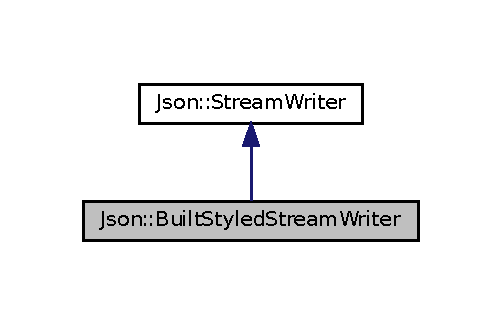
\includegraphics[width=241pt]{structJson_1_1BuiltStyledStreamWriter__inherit__graph}
\end{center}
\end{figure}


Collaboration diagram for Json\+:\+:Built\+Styled\+Stream\+Writer\+:
\nopagebreak
\begin{figure}[H]
\begin{center}
\leavevmode
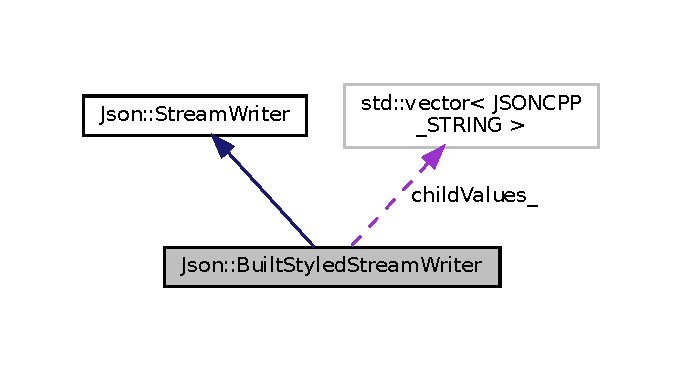
\includegraphics[width=241pt]{structJson_1_1BuiltStyledStreamWriter__coll__graph}
\end{center}
\end{figure}
\subsection*{Public Member Functions}
\begin{DoxyCompactItemize}
\item 
\mbox{\Hypertarget{structJson_1_1BuiltStyledStreamWriter_a69c46ddeca7a524734ae2be0866a4d98}\label{structJson_1_1BuiltStyledStreamWriter_a69c46ddeca7a524734ae2be0866a4d98}} 
{\bfseries Built\+Styled\+Stream\+Writer} (J\+S\+O\+N\+C\+P\+P\+\_\+\+S\+T\+R\+I\+NG const \&indentation, \hyperlink{structJson_1_1CommentStyle_a51fc08f3518fd81eba12f340d19a3d0c}{Comment\+Style\+::\+Enum} cs, J\+S\+O\+N\+C\+P\+P\+\_\+\+S\+T\+R\+I\+NG const \&colon\+Symbol, J\+S\+O\+N\+C\+P\+P\+\_\+\+S\+T\+R\+I\+NG const \&null\+Symbol, J\+S\+O\+N\+C\+P\+P\+\_\+\+S\+T\+R\+I\+NG const \&ending\+Line\+Feed\+Symbol, bool use\+Special\+Floats, unsigned int precision, \hyperlink{namespaceJson_af6e1447a3c43e3a62e11050dd0a11ce8}{Precision\+Type} precision\+Type)
\item 
int \hyperlink{structJson_1_1BuiltStyledStreamWriter_a823cdb1afabb6b0d5f39bcd5a6a6f747}{write} (\hyperlink{classJson_1_1Value}{Value} const \&root, J\+S\+O\+N\+C\+P\+P\+\_\+\+O\+S\+T\+R\+E\+AM $\ast$sout) J\+S\+O\+N\+C\+P\+P\+\_\+\+O\+V\+E\+R\+R\+I\+DE
\end{DoxyCompactItemize}
\subsection*{Additional Inherited Members}


\subsection{Member Function Documentation}
\mbox{\Hypertarget{structJson_1_1BuiltStyledStreamWriter_a823cdb1afabb6b0d5f39bcd5a6a6f747}\label{structJson_1_1BuiltStyledStreamWriter_a823cdb1afabb6b0d5f39bcd5a6a6f747}} 
\index{Json\+::\+Built\+Styled\+Stream\+Writer@{Json\+::\+Built\+Styled\+Stream\+Writer}!write@{write}}
\index{write@{write}!Json\+::\+Built\+Styled\+Stream\+Writer@{Json\+::\+Built\+Styled\+Stream\+Writer}}
\subsubsection{\texorpdfstring{write()}{write()}}
{\footnotesize\ttfamily int Json\+::\+Built\+Styled\+Stream\+Writer\+::write (\begin{DoxyParamCaption}\item[{\hyperlink{classJson_1_1Value}{Value} const \&}]{root,  }\item[{J\+S\+O\+N\+C\+P\+P\+\_\+\+O\+S\+T\+R\+E\+AM $\ast$}]{sout }\end{DoxyParamCaption})\hspace{0.3cm}{\ttfamily [virtual]}}

Write \hyperlink{classJson_1_1Value}{Value} into document as configured in sub-\/class. Do not take ownership of sout, but maintain a reference during function. \begin{DoxyPrecond}{Precondition}
sout != N\+U\+LL 
\end{DoxyPrecond}
\begin{DoxyReturn}{Returns}
zero on success (For now, we always return zero, so check the stream instead.) 
\end{DoxyReturn}

\begin{DoxyExceptions}{Exceptions}
{\em std\+::exception} & possibly, depending on configuration \\
\hline
\end{DoxyExceptions}


Implements \hyperlink{classJson_1_1StreamWriter_a84278bad0c9a9fc587bc2a97c5bb5993}{Json\+::\+Stream\+Writer}.



The documentation for this struct was generated from the following file\+:\begin{DoxyCompactItemize}
\item 
/home/mjonsson/repo/cpp\+Adv/media\+F\+W/src/jsoncpp.\+cpp\end{DoxyCompactItemize}

\hypertarget{classJson_1_1CharReader}{}\section{Json\+:\+:Char\+Reader Class Reference}
\label{classJson_1_1CharReader}\index{Json\+::\+Char\+Reader@{Json\+::\+Char\+Reader}}


{\ttfamily \#include $<$json.\+h$>$}



Inheritance diagram for Json\+:\+:Char\+Reader\+:
\nopagebreak
\begin{figure}[H]
\begin{center}
\leavevmode
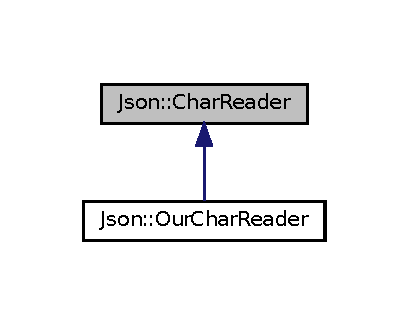
\includegraphics[width=196pt]{classJson_1_1CharReader__inherit__graph}
\end{center}
\end{figure}
\subsection*{Classes}
\begin{DoxyCompactItemize}
\item 
class \hyperlink{classJson_1_1CharReader_1_1Factory}{Factory}
\end{DoxyCompactItemize}
\subsection*{Public Member Functions}
\begin{DoxyCompactItemize}
\item 
virtual bool \hyperlink{classJson_1_1CharReader_a7983680d50fd0745f371c43b162e78e1}{parse} (char const $\ast$begin\+Doc, char const $\ast$end\+Doc, \hyperlink{classJson_1_1Value}{Value} $\ast$root, J\+S\+O\+N\+C\+P\+P\+\_\+\+S\+T\+R\+I\+NG $\ast$errs)=0
\begin{DoxyCompactList}\small\item\em Read a \hyperlink{classJson_1_1Value}{Value} from a \href{http://www.json.org}{\tt J\+S\+ON} document. The document must be a U\+T\+F-\/8 encoded string containing the document to read. \end{DoxyCompactList}\end{DoxyCompactItemize}


\subsection{Detailed Description}
Interface for reading J\+S\+ON from a char array. 

\subsection{Member Function Documentation}
\mbox{\Hypertarget{classJson_1_1CharReader_a7983680d50fd0745f371c43b162e78e1}\label{classJson_1_1CharReader_a7983680d50fd0745f371c43b162e78e1}} 
\index{Json\+::\+Char\+Reader@{Json\+::\+Char\+Reader}!parse@{parse}}
\index{parse@{parse}!Json\+::\+Char\+Reader@{Json\+::\+Char\+Reader}}
\subsubsection{\texorpdfstring{parse()}{parse()}}
{\footnotesize\ttfamily virtual bool Json\+::\+Char\+Reader\+::parse (\begin{DoxyParamCaption}\item[{char const $\ast$}]{begin\+Doc,  }\item[{char const $\ast$}]{end\+Doc,  }\item[{\hyperlink{classJson_1_1Value}{Value} $\ast$}]{root,  }\item[{J\+S\+O\+N\+C\+P\+P\+\_\+\+S\+T\+R\+I\+NG $\ast$}]{errs }\end{DoxyParamCaption})\hspace{0.3cm}{\ttfamily [pure virtual]}}



Read a \hyperlink{classJson_1_1Value}{Value} from a \href{http://www.json.org}{\tt J\+S\+ON} document. The document must be a U\+T\+F-\/8 encoded string containing the document to read. 


\begin{DoxyParams}{Parameters}
{\em begin\+Doc} & Pointer on the beginning of the U\+T\+F-\/8 encoded string of the document to read. \\
\hline
{\em end\+Doc} & Pointer on the end of the U\+T\+F-\/8 encoded string of the document to read. Must be $>$= begin\+Doc. \\
\hline
{\em root} & \mbox{[}out\mbox{]} Contains the root value of the document if it was successfully parsed. \\
\hline
{\em errs} & \mbox{[}out\mbox{]} Formatted error messages (if not N\+U\+LL) a user friendly string that lists errors in the parsed document. \\
\hline
\end{DoxyParams}
\begin{DoxyReturn}{Returns}
{\ttfamily true} if the document was successfully parsed, {\ttfamily false} if an error occurred. 
\end{DoxyReturn}


Implemented in \hyperlink{classJson_1_1OurCharReader_a547f08ec5a9951ca69e8bb2e90296c83}{Json\+::\+Our\+Char\+Reader}.



The documentation for this class was generated from the following file\+:\begin{DoxyCompactItemize}
\item 
/home/mjonsson/repo/cpp\+Adv/media\+F\+W/inc/json/json.\+h\end{DoxyCompactItemize}

\hypertarget{classJson_1_1CharReaderBuilder}{}\section{Json\+:\+:Char\+Reader\+Builder Class Reference}
\label{classJson_1_1CharReaderBuilder}\index{Json\+::\+Char\+Reader\+Builder@{Json\+::\+Char\+Reader\+Builder}}


Build a \hyperlink{classJson_1_1CharReader}{Char\+Reader} implementation.  




{\ttfamily \#include $<$json.\+h$>$}



Inheritance diagram for Json\+:\+:Char\+Reader\+Builder\+:
\nopagebreak
\begin{figure}[H]
\begin{center}
\leavevmode
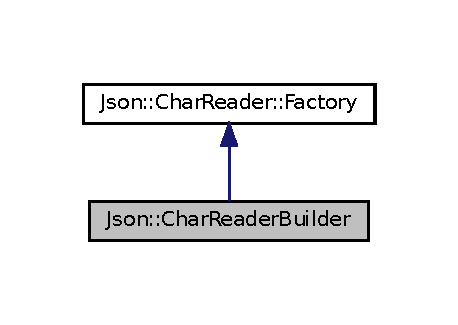
\includegraphics[width=220pt]{classJson_1_1CharReaderBuilder__inherit__graph}
\end{center}
\end{figure}


Collaboration diagram for Json\+:\+:Char\+Reader\+Builder\+:
\nopagebreak
\begin{figure}[H]
\begin{center}
\leavevmode
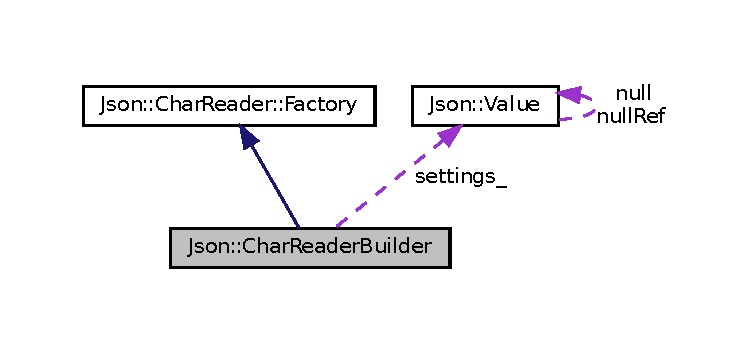
\includegraphics[width=350pt]{classJson_1_1CharReaderBuilder__coll__graph}
\end{center}
\end{figure}
\subsection*{Public Member Functions}
\begin{DoxyCompactItemize}
\item 
\hyperlink{classJson_1_1CharReader}{Char\+Reader} $\ast$ \hyperlink{classJson_1_1CharReaderBuilder_a3a262fcc76c1eb8eebfd4718fb4e9722}{new\+Char\+Reader} () const J\+S\+O\+N\+C\+P\+P\+\_\+\+O\+V\+E\+R\+R\+I\+DE
\begin{DoxyCompactList}\small\item\em Allocate a \hyperlink{classJson_1_1CharReader}{Char\+Reader} via operator new(). \end{DoxyCompactList}\item 
bool \hyperlink{classJson_1_1CharReaderBuilder_af890b5cb70e9b372e41de5c9e6535d21}{validate} (\hyperlink{classJson_1_1Value}{Json\+::\+Value} $\ast$invalid) const
\item 
\hyperlink{classJson_1_1Value}{Value} \& \hyperlink{classJson_1_1CharReaderBuilder_a84b35ef443340c06c0aa7b47851d8d86}{operator\mbox{[}$\,$\mbox{]}} (J\+S\+O\+N\+C\+P\+P\+\_\+\+S\+T\+R\+I\+NG key)
\end{DoxyCompactItemize}
\subsection*{Static Public Member Functions}
\begin{DoxyCompactItemize}
\item 
static void \hyperlink{classJson_1_1CharReaderBuilder_a03ff031e06aabff989ab4addc87294ab}{set\+Defaults} (\hyperlink{classJson_1_1Value}{Json\+::\+Value} $\ast$settings)
\item 
static void \hyperlink{classJson_1_1CharReaderBuilder_a9c19e3c5475f9072d527810d4bf56749}{strict\+Mode} (\hyperlink{classJson_1_1Value}{Json\+::\+Value} $\ast$settings)
\end{DoxyCompactItemize}
\subsection*{Public Attributes}
\begin{DoxyCompactItemize}
\item 
\hyperlink{classJson_1_1Value}{Json\+::\+Value} \hyperlink{classJson_1_1CharReaderBuilder_ac69b7911ad64c171c51ebaf2ea26d958}{settings\+\_\+}
\end{DoxyCompactItemize}


\subsection{Detailed Description}
Build a \hyperlink{classJson_1_1CharReader}{Char\+Reader} implementation. 

Usage\+: 
\begin{DoxyCode}
\textcolor{keyword}{using namespace }\hyperlink{namespaceJson}{Json};
\hyperlink{classJson_1_1CharReaderBuilder}{CharReaderBuilder} builder;
builder[\textcolor{stringliteral}{"collectComments"}] = \textcolor{keyword}{false};
\hyperlink{classJson_1_1Value}{Value} value;
JSONCPP\_STRING errs;
\textcolor{keywordtype}{bool} ok = \hyperlink{namespaceJson_aab0cf1ecf81d1aeca12be2a416a84352}{parseFromStream}(builder, std::cin, &value, &errs);
\end{DoxyCode}
 

\subsection{Member Function Documentation}
\mbox{\Hypertarget{classJson_1_1CharReaderBuilder_a3a262fcc76c1eb8eebfd4718fb4e9722}\label{classJson_1_1CharReaderBuilder_a3a262fcc76c1eb8eebfd4718fb4e9722}} 
\index{Json\+::\+Char\+Reader\+Builder@{Json\+::\+Char\+Reader\+Builder}!new\+Char\+Reader@{new\+Char\+Reader}}
\index{new\+Char\+Reader@{new\+Char\+Reader}!Json\+::\+Char\+Reader\+Builder@{Json\+::\+Char\+Reader\+Builder}}
\subsubsection{\texorpdfstring{new\+Char\+Reader()}{newCharReader()}}
{\footnotesize\ttfamily \hyperlink{classJson_1_1CharReader}{Char\+Reader} $\ast$ Json\+::\+Char\+Reader\+Builder\+::new\+Char\+Reader (\begin{DoxyParamCaption}{ }\end{DoxyParamCaption}) const\hspace{0.3cm}{\ttfamily [virtual]}}



Allocate a \hyperlink{classJson_1_1CharReader}{Char\+Reader} via operator new(). 


\begin{DoxyExceptions}{Exceptions}
{\em std\+::exception} & if something goes wrong (e.\+g. invalid settings) \\
\hline
\end{DoxyExceptions}


Implements \hyperlink{classJson_1_1CharReader_1_1Factory_a4c5862a1ffd432372dbe65cf59de98c4}{Json\+::\+Char\+Reader\+::\+Factory}.

\mbox{\Hypertarget{classJson_1_1CharReaderBuilder_a84b35ef443340c06c0aa7b47851d8d86}\label{classJson_1_1CharReaderBuilder_a84b35ef443340c06c0aa7b47851d8d86}} 
\index{Json\+::\+Char\+Reader\+Builder@{Json\+::\+Char\+Reader\+Builder}!operator\mbox{[}\mbox{]}@{operator[]}}
\index{operator\mbox{[}\mbox{]}@{operator[]}!Json\+::\+Char\+Reader\+Builder@{Json\+::\+Char\+Reader\+Builder}}
\subsubsection{\texorpdfstring{operator[]()}{operator[]()}}
{\footnotesize\ttfamily \hyperlink{classJson_1_1Value}{Value} \& Json\+::\+Char\+Reader\+Builder\+::operator\mbox{[}$\,$\mbox{]} (\begin{DoxyParamCaption}\item[{J\+S\+O\+N\+C\+P\+P\+\_\+\+S\+T\+R\+I\+NG}]{key }\end{DoxyParamCaption})}

A simple way to update a specific setting. \mbox{\Hypertarget{classJson_1_1CharReaderBuilder_a03ff031e06aabff989ab4addc87294ab}\label{classJson_1_1CharReaderBuilder_a03ff031e06aabff989ab4addc87294ab}} 
\index{Json\+::\+Char\+Reader\+Builder@{Json\+::\+Char\+Reader\+Builder}!set\+Defaults@{set\+Defaults}}
\index{set\+Defaults@{set\+Defaults}!Json\+::\+Char\+Reader\+Builder@{Json\+::\+Char\+Reader\+Builder}}
\subsubsection{\texorpdfstring{set\+Defaults()}{setDefaults()}}
{\footnotesize\ttfamily void Json\+::\+Char\+Reader\+Builder\+::set\+Defaults (\begin{DoxyParamCaption}\item[{\hyperlink{classJson_1_1Value}{Json\+::\+Value} $\ast$}]{settings }\end{DoxyParamCaption})\hspace{0.3cm}{\ttfamily [static]}}

Called by ctor, but you can use this to reset settings\+\_\+. \begin{DoxyPrecond}{Precondition}
\textquotesingle{}settings\textquotesingle{} != N\+U\+LL (but Json\+::null is fine) 
\end{DoxyPrecond}
\begin{DoxyRemark}{Remarks}
Defaults\+: 
\begin{DoxyCodeInclude}
\end{DoxyCodeInclude}

\end{DoxyRemark}
\mbox{[}Char\+Reader\+Builder\+Defaults\mbox{]}

\mbox{[}Char\+Reader\+Builder\+Defaults\mbox{]} \mbox{\Hypertarget{classJson_1_1CharReaderBuilder_a9c19e3c5475f9072d527810d4bf56749}\label{classJson_1_1CharReaderBuilder_a9c19e3c5475f9072d527810d4bf56749}} 
\index{Json\+::\+Char\+Reader\+Builder@{Json\+::\+Char\+Reader\+Builder}!strict\+Mode@{strict\+Mode}}
\index{strict\+Mode@{strict\+Mode}!Json\+::\+Char\+Reader\+Builder@{Json\+::\+Char\+Reader\+Builder}}
\subsubsection{\texorpdfstring{strict\+Mode()}{strictMode()}}
{\footnotesize\ttfamily void Json\+::\+Char\+Reader\+Builder\+::strict\+Mode (\begin{DoxyParamCaption}\item[{\hyperlink{classJson_1_1Value}{Json\+::\+Value} $\ast$}]{settings }\end{DoxyParamCaption})\hspace{0.3cm}{\ttfamily [static]}}

Same as old \hyperlink{classJson_1_1Features_ae23176c14b2e79e81fb61fb1a8ab58ee}{Features\+::strict\+Mode()}. \begin{DoxyPrecond}{Precondition}
\textquotesingle{}settings\textquotesingle{} != N\+U\+LL (but Json\+::null is fine) 
\end{DoxyPrecond}
\begin{DoxyRemark}{Remarks}
Defaults\+: 
\begin{DoxyCodeInclude}
\end{DoxyCodeInclude}

\end{DoxyRemark}
\mbox{[}Char\+Reader\+Builder\+Strict\+Mode\mbox{]}

\mbox{[}Char\+Reader\+Builder\+Strict\+Mode\mbox{]} \mbox{\Hypertarget{classJson_1_1CharReaderBuilder_af890b5cb70e9b372e41de5c9e6535d21}\label{classJson_1_1CharReaderBuilder_af890b5cb70e9b372e41de5c9e6535d21}} 
\index{Json\+::\+Char\+Reader\+Builder@{Json\+::\+Char\+Reader\+Builder}!validate@{validate}}
\index{validate@{validate}!Json\+::\+Char\+Reader\+Builder@{Json\+::\+Char\+Reader\+Builder}}
\subsubsection{\texorpdfstring{validate()}{validate()}}
{\footnotesize\ttfamily bool Json\+::\+Char\+Reader\+Builder\+::validate (\begin{DoxyParamCaption}\item[{\hyperlink{classJson_1_1Value}{Json\+::\+Value} $\ast$}]{invalid }\end{DoxyParamCaption}) const}

\begin{DoxyReturn}{Returns}
true if \textquotesingle{}settings\textquotesingle{} are legal and consistent; otherwise, indicate bad settings via \textquotesingle{}invalid\textquotesingle{}. 
\end{DoxyReturn}


\subsection{Member Data Documentation}
\mbox{\Hypertarget{classJson_1_1CharReaderBuilder_ac69b7911ad64c171c51ebaf2ea26d958}\label{classJson_1_1CharReaderBuilder_ac69b7911ad64c171c51ebaf2ea26d958}} 
\index{Json\+::\+Char\+Reader\+Builder@{Json\+::\+Char\+Reader\+Builder}!settings\+\_\+@{settings\+\_\+}}
\index{settings\+\_\+@{settings\+\_\+}!Json\+::\+Char\+Reader\+Builder@{Json\+::\+Char\+Reader\+Builder}}
\subsubsection{\texorpdfstring{settings\+\_\+}{settings\_}}
{\footnotesize\ttfamily \hyperlink{classJson_1_1Value}{Json\+::\+Value} Json\+::\+Char\+Reader\+Builder\+::settings\+\_\+}

Configuration of this builder. These are case-\/sensitive. Available settings (case-\/sensitive)\+:
\begin{DoxyItemize}
\item {\ttfamily \char`\"{}collect\+Comments\char`\"{}\+: false or true}
\begin{DoxyItemize}
\item true to collect comment and allow writing them back during serialization, false to discard comments. This parameter is ignored if allow\+Comments is false.
\end{DoxyItemize}
\item {\ttfamily \char`\"{}allow\+Comments\char`\"{}\+: false or true}
\begin{DoxyItemize}
\item true if comments are allowed.
\end{DoxyItemize}
\item {\ttfamily \char`\"{}strict\+Root\char`\"{}\+: false or true}
\begin{DoxyItemize}
\item true if root must be either an array or an object value
\end{DoxyItemize}
\item {\ttfamily \char`\"{}allow\+Dropped\+Null\+Placeholders\char`\"{}\+: false or true}
\begin{DoxyItemize}
\item true if dropped null placeholders are allowed. (See \hyperlink{classJson_1_1StreamWriterBuilder}{Stream\+Writer\+Builder}.)
\end{DoxyItemize}
\item {\ttfamily \char`\"{}allow\+Numeric\+Keys\char`\"{}\+: false or true}
\begin{DoxyItemize}
\item true if numeric object keys are allowed.
\end{DoxyItemize}
\item {\ttfamily \char`\"{}allow\+Single\+Quotes\char`\"{}\+: false or true}
\begin{DoxyItemize}
\item true if \textquotesingle{}\textquotesingle{} are allowed for strings (both keys and values)
\end{DoxyItemize}
\item {\ttfamily \char`\"{}stack\+Limit\char`\"{}\+: integer}
\begin{DoxyItemize}
\item Exceeding stack\+Limit (recursive depth of {\ttfamily read\+Value()}) will cause an exception.
\item This is a security issue (seg-\/faults caused by deeply nested J\+S\+ON), so the default is low.
\end{DoxyItemize}
\item {\ttfamily \char`\"{}fail\+If\+Extra\char`\"{}\+: false or true}
\begin{DoxyItemize}
\item If true, {\ttfamily parse()} returns false when extra non-\/whitespace trails the J\+S\+ON value in the input string.
\end{DoxyItemize}
\item {\ttfamily \char`\"{}reject\+Dup\+Keys\char`\"{}\+: false or true}
\begin{DoxyItemize}
\item If true, {\ttfamily parse()} returns false when a key is duplicated within an object.
\end{DoxyItemize}
\item {\ttfamily \char`\"{}allow\+Special\+Floats\char`\"{}\+: false or true}
\begin{DoxyItemize}
\item If true, special float values (Na\+Ns and infinities) are allowed and their values are lossfree restorable.
\end{DoxyItemize}
\end{DoxyItemize}

You can examine \textquotesingle{}settings\+\_\+` yourself to see the defaults. You can also write and read them just like any J\+S\+ON \hyperlink{classJson_1_1Value}{Value}. \begin{DoxySeeAlso}{See also}
\hyperlink{classJson_1_1CharReaderBuilder_a03ff031e06aabff989ab4addc87294ab}{set\+Defaults()} 
\end{DoxySeeAlso}


The documentation for this class was generated from the following files\+:\begin{DoxyCompactItemize}
\item 
/home/mjonsson/repo/cpp\+Adv/media\+F\+W/inc/json/json.\+h\item 
/home/mjonsson/repo/cpp\+Adv/media\+F\+W/src/json/jsoncpp.\+cpp\end{DoxyCompactItemize}

\hypertarget{classCli}{}\section{Cli Class Reference}
\label{classCli}\index{Cli@{Cli}}


Module handling everything related to our Command line interface.  




{\ttfamily \#include \char`\"{}inc/\+Cli.\+h\char`\"{}}



Inheritance diagram for Cli\+:\nopagebreak
\begin{figure}[H]
\begin{center}
\leavevmode
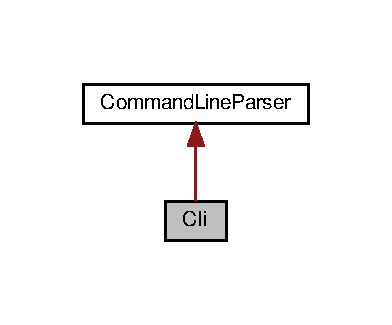
\includegraphics[width=188pt]{classCli__inherit__graph}
\end{center}
\end{figure}


Collaboration diagram for Cli\+:\nopagebreak
\begin{figure}[H]
\begin{center}
\leavevmode
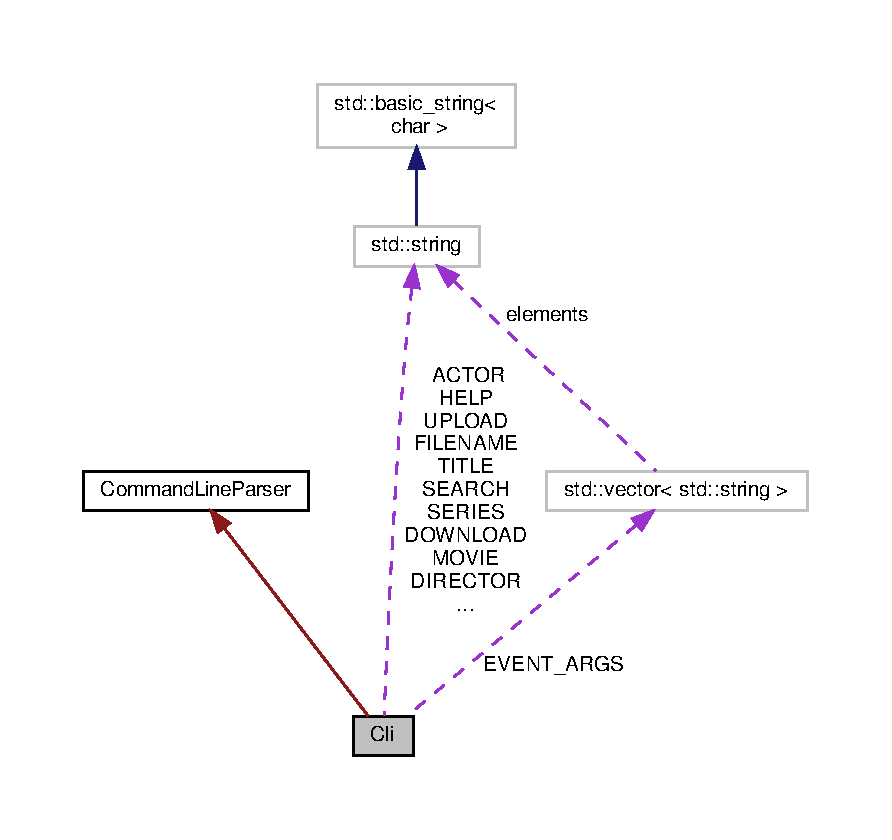
\includegraphics[width=350pt]{classCli__coll__graph}
\end{center}
\end{figure}
\subsection*{Public Member Functions}
\begin{DoxyCompactItemize}
\item 
\hyperlink{classRequest}{Request} \hyperlink{classCli_aa2b3675ef3e3bb01ed0d1997460a0e28}{process} () override
\begin{DoxyCompactList}\small\item\em Public method processing input from stdin. . \end{DoxyCompactList}\item 
\hyperlink{classRequest}{Request} \hyperlink{classCli_af29a5d8a0c3863f69c0e21133dee2d1b}{interprete} (std\+::vector$<$ std\+::string $>$ \&) override
\begin{DoxyCompactList}\small\item\em translate incoming user request and save in request object \end{DoxyCompactList}\item 
\hyperlink{classRequest}{Request} \hyperlink{classCli_a4ee41556f8c3a736d813f0d937413da0}{process} (std\+::string \&) override
\begin{DoxyCompactList}\small\item\em Public method processing input from stdin. \end{DoxyCompactList}\item 
\mbox{\Hypertarget{classCli_af21370e0e274a657bf2c9efceb18b6b3}\label{classCli_af21370e0e274a657bf2c9efceb18b6b3}} 
void {\bfseries verify\+Upload\+Test} (\hyperlink{classRequest}{Request} \&request, std\+::vector$<$ std\+::string $>$ \&i)
\end{DoxyCompactItemize}
\subsection*{Private Member Functions}
\begin{DoxyCompactItemize}
\item 
std\+::vector$<$ std\+::string $>$ \hyperlink{classCli_aaf60768f062a6dc2557aaddbe738a19c}{split} (std\+::string \&input, char delim)
\item 
\mbox{\Hypertarget{classCli_a8b6ecb803833139fc7dbdb1bac9cb127}\label{classCli_a8b6ecb803833139fc7dbdb1bac9cb127}} 
int {\bfseries check\+Valid\+Event} (std\+::vector$<$ std\+::string $>$ \&input, Event \&event)
\item 
\mbox{\Hypertarget{classCli_a116a3c89cbb5f9b807661123ee0dd5a3}\label{classCli_a116a3c89cbb5f9b807661123ee0dd5a3}} 
int {\bfseries check\+Valid\+Category} (std\+::vector$<$ std\+::string $>$ \&input, Category \&category)
\item 
\mbox{\Hypertarget{classCli_a5137618fd0eeaa34964b175aff8061ef}\label{classCli_a5137618fd0eeaa34964b175aff8061ef}} 
int {\bfseries check\+Valid\+Type} (\hyperlink{classRequest}{Request} \&request, std\+::string \&type)
\item 
\mbox{\Hypertarget{classCli_af10df67ce26c8a773e573323c47d9781}\label{classCli_af10df67ce26c8a773e573323c47d9781}} 
int {\bfseries verify\+Object\+Exists} (Category \&category, const std\+::string \&value)
\item 
\mbox{\Hypertarget{classCli_a6121ca606d1ae7b8b8b57d31786d2e18}\label{classCli_a6121ca606d1ae7b8b8b57d31786d2e18}} 
int {\bfseries get\+Type\+Of\+Value} (std\+::vector$<$ std\+::string $>$ \&input, std\+::string \&type)
\item 
\mbox{\Hypertarget{classCli_ac00196cbc1bd9683127923b13de9cbbc}\label{classCli_ac00196cbc1bd9683127923b13de9cbbc}} 
int {\bfseries get\+Value\+Of\+Type} (std\+::vector$<$ std\+::string $>$ \&input, std\+::string \&val)
\item 
\mbox{\Hypertarget{classCli_a2e2d57f7175aa6423db2a616098a3b2e}\label{classCli_a2e2d57f7175aa6423db2a616098a3b2e}} 
void {\bfseries set\+File\+Name} (\hyperlink{classRequest}{Request} \&request, std\+::string \&val)
\item 
\mbox{\Hypertarget{classCli_a0cf3263bf644c151d59b8957746a9507}\label{classCli_a0cf3263bf644c151d59b8957746a9507}} 
void {\bfseries set\+Properties} (\hyperlink{classRequest}{Request} \&request, std\+::vector$<$ std\+::string $>$ \&item)
\item 
\mbox{\Hypertarget{classCli_ae51022f0ca5e385ebd2551021f653b97}\label{classCli_ae51022f0ca5e385ebd2551021f653b97}} 
int {\bfseries verify\+Upload} (\hyperlink{classRequest}{Request} \&request)
\item 
void \hyperlink{classCli_a8251d6c89698aaf128318fc3ad4b2906}{print\+Options} ()
\begin{DoxyCompactList}\small\item\em Test A private method that prints all valid options for stdin. \end{DoxyCompactList}\end{DoxyCompactItemize}
\subsection*{Private Attributes}
\begin{DoxyCompactItemize}
\item 
\mbox{\Hypertarget{classCli_a6b39501d775b2719cdacd6937507906a}\label{classCli_a6b39501d775b2719cdacd6937507906a}} 
const std\+::string {\bfseries T\+I\+T\+LE} = \char`\"{}title\char`\"{}
\item 
\mbox{\Hypertarget{classCli_ae49ac3e6fb12dfa20c41ca189cbcd863}\label{classCli_ae49ac3e6fb12dfa20c41ca189cbcd863}} 
const std\+::string {\bfseries G\+E\+N\+RE} = \char`\"{}genre\char`\"{}
\item 
\mbox{\Hypertarget{classCli_af1bfe00ff8a3f8415e74b39970007f1b}\label{classCli_af1bfe00ff8a3f8415e74b39970007f1b}} 
const std\+::string {\bfseries A\+C\+T\+OR} = \char`\"{}actor\char`\"{}
\item 
\mbox{\Hypertarget{classCli_ae1510a4c9ae1696862bf6362eddfdb63}\label{classCli_ae1510a4c9ae1696862bf6362eddfdb63}} 
const std\+::string {\bfseries D\+I\+R\+E\+C\+T\+OR} = \char`\"{}director\char`\"{}
\item 
\mbox{\Hypertarget{classCli_a25d22c371e6d1a701a375dd77b98a839}\label{classCli_a25d22c371e6d1a701a375dd77b98a839}} 
const std\+::string {\bfseries F\+I\+L\+E\+N\+A\+ME} = \char`\"{}filename\char`\"{}
\item 
\mbox{\Hypertarget{classCli_a74a219ff6c475389cbcffaeaad0f0315}\label{classCli_a74a219ff6c475389cbcffaeaad0f0315}} 
std\+::string {\bfseries M\+O\+V\+IE} = \char`\"{}movie\char`\"{}
\item 
\mbox{\Hypertarget{classCli_a9e046dc850ddd6b5ee7da84655df7ad6}\label{classCli_a9e046dc850ddd6b5ee7da84655df7ad6}} 
std\+::string {\bfseries S\+E\+R\+I\+ES} = \char`\"{}series\char`\"{}
\item 
\mbox{\Hypertarget{classCli_a45bb315b7351264e545e257ad09adbe8}\label{classCli_a45bb315b7351264e545e257ad09adbe8}} 
const std\+::string {\bfseries D\+O\+W\+N\+L\+O\+AD} = \char`\"{}download\char`\"{}
\item 
\mbox{\Hypertarget{classCli_ad97f44e157d1e1919f24a51f503b8ad6}\label{classCli_ad97f44e157d1e1919f24a51f503b8ad6}} 
const std\+::string {\bfseries U\+P\+L\+O\+AD} = \char`\"{}upload\char`\"{}
\item 
\mbox{\Hypertarget{classCli_a6689cd38c78d1d3f06da4fc036d5a405}\label{classCli_a6689cd38c78d1d3f06da4fc036d5a405}} 
const std\+::string {\bfseries S\+E\+A\+R\+CH} = \char`\"{}search\char`\"{}
\item 
\mbox{\Hypertarget{classCli_acca3f466bba719de9ac3a491e7aa02c8}\label{classCli_acca3f466bba719de9ac3a491e7aa02c8}} 
const std\+::string {\bfseries D\+E\+L\+E\+TE} = \char`\"{}delete\char`\"{}
\item 
\mbox{\Hypertarget{classCli_adf56775dc41676f404c6f83f48b92c95}\label{classCli_adf56775dc41676f404c6f83f48b92c95}} 
const std\+::string {\bfseries H\+E\+LP} = \char`\"{}help\char`\"{}
\item 
\mbox{\Hypertarget{classCli_a277fa8260456d4eda6fd69022c29f2fe}\label{classCli_a277fa8260456d4eda6fd69022c29f2fe}} 
const std\+::string {\bfseries E\+X\+IT} = \char`\"{}exit\char`\"{}
\item 
\mbox{\Hypertarget{classCli_a3610685c550060a08adb0fd78ee6866e}\label{classCli_a3610685c550060a08adb0fd78ee6866e}} 
const std\+::vector$<$ std\+::string $>$ {\bfseries E\+V\+E\+N\+T\+\_\+\+A\+R\+GS} = \{U\+P\+L\+O\+AD, D\+O\+W\+N\+L\+O\+AD, S\+E\+A\+R\+CH, D\+E\+L\+E\+TE, H\+E\+LP, E\+X\+IT\}
\end{DoxyCompactItemize}


\subsection{Detailed Description}
Module handling everything related to our Command line interface. 

Class implementing the functionality of a command line interface.

Receives inputs from S\+T\+D\+IN and splits the result into strings. 

\subsection{Member Function Documentation}
\mbox{\Hypertarget{classCli_af29a5d8a0c3863f69c0e21133dee2d1b}\label{classCli_af29a5d8a0c3863f69c0e21133dee2d1b}} 
\index{Cli@{Cli}!interprete@{interprete}}
\index{interprete@{interprete}!Cli@{Cli}}
\subsubsection{\texorpdfstring{interprete()}{interprete()}}
{\footnotesize\ttfamily \hyperlink{classRequest}{Request} Cli\+::interprete (\begin{DoxyParamCaption}\item[{std\+::vector$<$ std\+::string $>$ \&}]{input }\end{DoxyParamCaption})\hspace{0.3cm}{\ttfamily [override]}, {\ttfamily [virtual]}}



translate incoming user request and save in request object 

Client\+::interprete interface of \hyperlink{classCommandLineParser}{Command\+Line\+Parser} 
\begin{DoxyParams}{Parameters}
{\em std\+::vector$<$std\+::string$>$\&} & vector of string arguments to be translated \\
\hline
\end{DoxyParams}
\begin{DoxyReturn}{Returns}
the translated request object 
\end{DoxyReturn}


Implements \hyperlink{classCommandLineParser}{Command\+Line\+Parser}.

Here is the caller graph for this function\+:\nopagebreak
\begin{figure}[H]
\begin{center}
\leavevmode
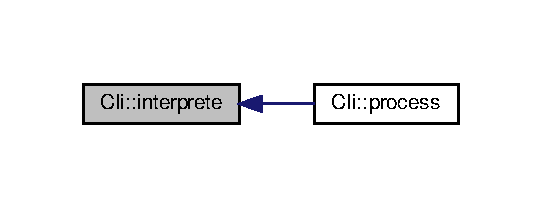
\includegraphics[width=260pt]{classCli_af29a5d8a0c3863f69c0e21133dee2d1b_icgraph}
\end{center}
\end{figure}
\mbox{\Hypertarget{classCli_a8251d6c89698aaf128318fc3ad4b2906}\label{classCli_a8251d6c89698aaf128318fc3ad4b2906}} 
\index{Cli@{Cli}!print\+Options@{print\+Options}}
\index{print\+Options@{print\+Options}!Cli@{Cli}}
\subsubsection{\texorpdfstring{print\+Options()}{printOptions()}}
{\footnotesize\ttfamily void Cli\+::print\+Options (\begin{DoxyParamCaption}{ }\end{DoxyParamCaption})\hspace{0.3cm}{\ttfamily [inline]}, {\ttfamily [private]}}



Test A private method that prints all valid options for stdin. 

\hyperlink{classCli_a8251d6c89698aaf128318fc3ad4b2906}{Cli\+::print\+Options} Here is the caller graph for this function\+:\nopagebreak
\begin{figure}[H]
\begin{center}
\leavevmode
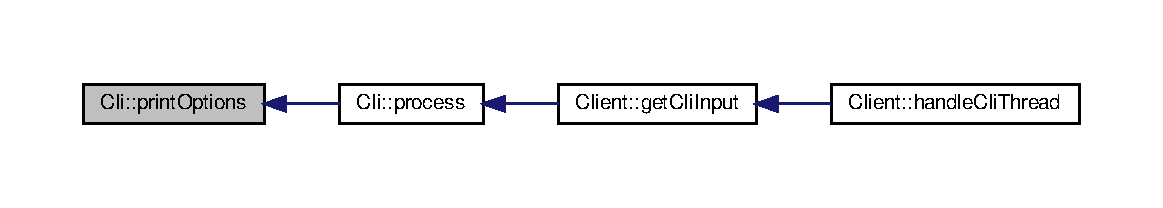
\includegraphics[width=350pt]{classCli_a8251d6c89698aaf128318fc3ad4b2906_icgraph}
\end{center}
\end{figure}
\mbox{\Hypertarget{classCli_aa2b3675ef3e3bb01ed0d1997460a0e28}\label{classCli_aa2b3675ef3e3bb01ed0d1997460a0e28}} 
\index{Cli@{Cli}!process@{process}}
\index{process@{process}!Cli@{Cli}}
\subsubsection{\texorpdfstring{process()}{process()}\hspace{0.1cm}{\footnotesize\ttfamily [1/2]}}
{\footnotesize\ttfamily \hyperlink{classRequest}{Request} Cli\+::process (\begin{DoxyParamCaption}{ }\end{DoxyParamCaption})\hspace{0.3cm}{\ttfamily [override]}, {\ttfamily [virtual]}}



Public method processing input from stdin. . 

Client\+::process() interface of \hyperlink{classCommandLineParser}{Command\+Line\+Parser} \begin{DoxyReturn}{Returns}
Vector of strings containing output from stdin. 
\end{DoxyReturn}


Implements \hyperlink{classCommandLineParser}{Command\+Line\+Parser}.

Here is the call graph for this function\+:\nopagebreak
\begin{figure}[H]
\begin{center}
\leavevmode
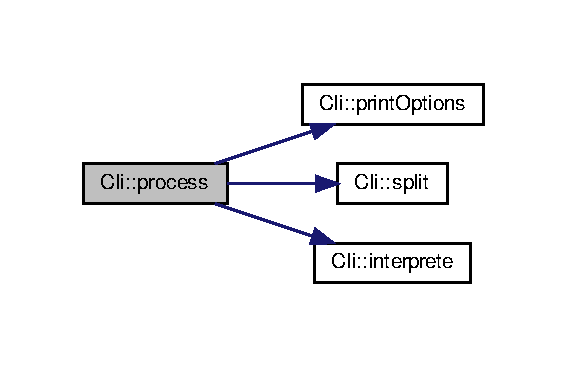
\includegraphics[width=272pt]{classCli_aa2b3675ef3e3bb01ed0d1997460a0e28_cgraph}
\end{center}
\end{figure}
Here is the caller graph for this function\+:\nopagebreak
\begin{figure}[H]
\begin{center}
\leavevmode
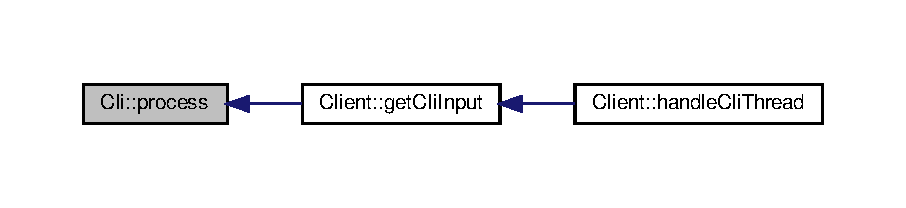
\includegraphics[width=350pt]{classCli_aa2b3675ef3e3bb01ed0d1997460a0e28_icgraph}
\end{center}
\end{figure}
\mbox{\Hypertarget{classCli_a4ee41556f8c3a736d813f0d937413da0}\label{classCli_a4ee41556f8c3a736d813f0d937413da0}} 
\index{Cli@{Cli}!process@{process}}
\index{process@{process}!Cli@{Cli}}
\subsubsection{\texorpdfstring{process()}{process()}\hspace{0.1cm}{\footnotesize\ttfamily [2/2]}}
{\footnotesize\ttfamily \hyperlink{classRequest}{Request} Cli\+::process (\begin{DoxyParamCaption}\item[{std\+::string \&}]{line }\end{DoxyParamCaption})\hspace{0.3cm}{\ttfamily [override]}, {\ttfamily [virtual]}}



Public method processing input from stdin. 

Client\+::process() interface of \hyperlink{classCommandLineParser}{Command\+Line\+Parser} 
\begin{DoxyParams}{Parameters}
{\em std\+::string\&} & fixed string used for unit testing mocking stdin \\
\hline
\end{DoxyParams}
\begin{DoxyReturn}{Returns}
Vector of strings containing output from stdin. 
\end{DoxyReturn}


Implements \hyperlink{classCommandLineParser}{Command\+Line\+Parser}.

Here is the call graph for this function\+:\nopagebreak
\begin{figure}[H]
\begin{center}
\leavevmode
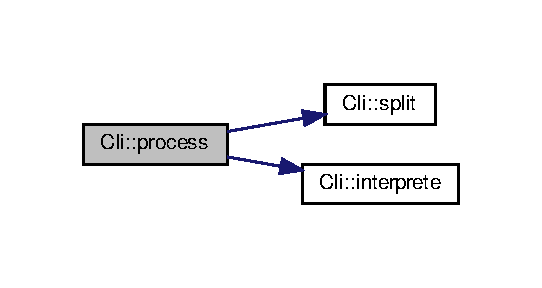
\includegraphics[width=260pt]{classCli_a4ee41556f8c3a736d813f0d937413da0_cgraph}
\end{center}
\end{figure}
\mbox{\Hypertarget{classCli_aaf60768f062a6dc2557aaddbe738a19c}\label{classCli_aaf60768f062a6dc2557aaddbe738a19c}} 
\index{Cli@{Cli}!split@{split}}
\index{split@{split}!Cli@{Cli}}
\subsubsection{\texorpdfstring{split()}{split()}}
{\footnotesize\ttfamily std\+::vector$<$std\+::string$>$ Cli\+::split (\begin{DoxyParamCaption}\item[{std\+::string \&}]{input,  }\item[{char}]{delim }\end{DoxyParamCaption})\hspace{0.3cm}{\ttfamily [inline]}, {\ttfamily [private]}}

\hyperlink{classCli_aaf60768f062a6dc2557aaddbe738a19c}{Cli\+::split}


\begin{DoxyParams}{Parameters}
{\em input} & incoming unprocessed string \\
\hline
{\em delim} & delimiter used to split \\
\hline
{\em input} & \\
\hline
\end{DoxyParams}
\begin{DoxyReturn}{Returns}

\end{DoxyReturn}

\begin{DoxyParams}{Parameters}
{\em input} & splitted into multiple strings saved in a std\+::vector \\
\hline
\end{DoxyParams}
Here is the caller graph for this function\+:\nopagebreak
\begin{figure}[H]
\begin{center}
\leavevmode
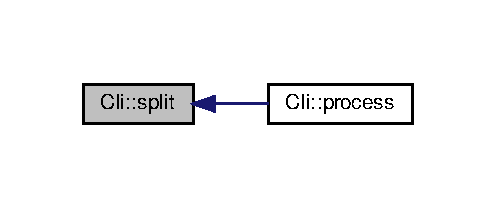
\includegraphics[width=238pt]{classCli_aaf60768f062a6dc2557aaddbe738a19c_icgraph}
\end{center}
\end{figure}


The documentation for this class was generated from the following files\+:\begin{DoxyCompactItemize}
\item 
inc/Cli.\+h\item 
src/Cli.\+cpp\end{DoxyCompactItemize}

\hypertarget{classClient}{}\section{Client Class Reference}
\label{classClient}\index{Client@{Client}}
\subsection*{Public Member Functions}
\begin{DoxyCompactItemize}
\item 
void \hyperlink{classClient_a33b0b1f7391689c68fa125549e8c5dcc}{setup} ()
\begin{DoxyCompactList}\small\item\em A method that waits C\+LI input from method get\+Cli\+Input. The method will break if input is interpreted as exit or continue by sending the request to be handled. \end{DoxyCompactList}\end{DoxyCompactItemize}
\subsection*{Public Attributes}
\begin{DoxyCompactItemize}
\item 
\mbox{\Hypertarget{classClient_a4c99f07fc4be08870e1067ba876e08fb}\label{classClient_a4c99f07fc4be08870e1067ba876e08fb}} 
Db\+Type {\bfseries type}
\end{DoxyCompactItemize}


\subsection{Member Function Documentation}
\mbox{\Hypertarget{classClient_a33b0b1f7391689c68fa125549e8c5dcc}\label{classClient_a33b0b1f7391689c68fa125549e8c5dcc}} 
\index{Client@{Client}!setup@{setup}}
\index{setup@{setup}!Client@{Client}}
\subsubsection{\texorpdfstring{setup()}{setup()}}
{\footnotesize\ttfamily void Client\+::setup (\begin{DoxyParamCaption}{ }\end{DoxyParamCaption})}



A method that waits C\+LI input from method get\+Cli\+Input. The method will break if input is interpreted as exit or continue by sending the request to be handled. 

\begin{DoxyReturn}{Returns}

\end{DoxyReturn}


The documentation for this class was generated from the following files\+:\begin{DoxyCompactItemize}
\item 
/home/mjonsson/repo/cpp\+Adv/media\+F\+W/inc/Client.\+h\item 
/home/mjonsson/repo/cpp\+Adv/media\+F\+W/src/Client.\+cpp\end{DoxyCompactItemize}

\hypertarget{structJson_1_1Value_1_1CommentInfo}{}\section{Json\+:\+:Value\+:\+:Comment\+Info Struct Reference}
\label{structJson_1_1Value_1_1CommentInfo}\index{Json\+::\+Value\+::\+Comment\+Info@{Json\+::\+Value\+::\+Comment\+Info}}
\subsection*{Public Member Functions}
\begin{DoxyCompactItemize}
\item 
\mbox{\Hypertarget{structJson_1_1Value_1_1CommentInfo_a4d01c2cd8c07995969c5d636dfd4fa8c}\label{structJson_1_1Value_1_1CommentInfo_a4d01c2cd8c07995969c5d636dfd4fa8c}} 
void {\bfseries set\+Comment} (const char $\ast$text, size\+\_\+t len)
\end{DoxyCompactItemize}
\subsection*{Public Attributes}
\begin{DoxyCompactItemize}
\item 
\mbox{\Hypertarget{structJson_1_1Value_1_1CommentInfo_a020f19c7098bab8ec8fec14cd1a5afb9}\label{structJson_1_1Value_1_1CommentInfo_a020f19c7098bab8ec8fec14cd1a5afb9}} 
char $\ast$ {\bfseries comment\+\_\+}
\end{DoxyCompactItemize}


The documentation for this struct was generated from the following files\+:\begin{DoxyCompactItemize}
\item 
/home/mjonsson/repo/cpp\+Adv/media\+F\+W/inc/json/json.\+h\item 
/home/mjonsson/repo/cpp\+Adv/media\+F\+W/src/json/jsoncpp.\+cpp\end{DoxyCompactItemize}

\hypertarget{structJson_1_1CommentStyle}{}\section{Json\+:\+:Comment\+Style Struct Reference}
\label{structJson_1_1CommentStyle}\index{Json\+::\+Comment\+Style@{Json\+::\+Comment\+Style}}


Scoped enums are not available until C++11.  


\subsection*{Public Types}
\begin{DoxyCompactItemize}
\item 
enum \hyperlink{structJson_1_1CommentStyle_a51fc08f3518fd81eba12f340d19a3d0c}{Enum} \{ \hyperlink{structJson_1_1CommentStyle_a51fc08f3518fd81eba12f340d19a3d0cac8b32a8bae63414c8647d4919da8d437}{None}, 
\hyperlink{structJson_1_1CommentStyle_a51fc08f3518fd81eba12f340d19a3d0cac65238f050773c107690a456e9c05c98}{Most}, 
\hyperlink{structJson_1_1CommentStyle_a51fc08f3518fd81eba12f340d19a3d0ca32302c0b97190c1808b3e38f367fef01}{All}
 \}\begin{DoxyCompactList}\small\item\em Decide whether to write comments. \end{DoxyCompactList}
\end{DoxyCompactItemize}


\subsection{Detailed Description}
Scoped enums are not available until C++11. 

\subsection{Member Enumeration Documentation}
\mbox{\Hypertarget{structJson_1_1CommentStyle_a51fc08f3518fd81eba12f340d19a3d0c}\label{structJson_1_1CommentStyle_a51fc08f3518fd81eba12f340d19a3d0c}} 
\index{Json\+::\+Comment\+Style@{Json\+::\+Comment\+Style}!Enum@{Enum}}
\index{Enum@{Enum}!Json\+::\+Comment\+Style@{Json\+::\+Comment\+Style}}
\subsubsection{\texorpdfstring{Enum}{Enum}}
{\footnotesize\ttfamily enum \hyperlink{structJson_1_1CommentStyle_a51fc08f3518fd81eba12f340d19a3d0c}{Json\+::\+Comment\+Style\+::\+Enum}}



Decide whether to write comments. 

\begin{DoxyEnumFields}{Enumerator}
\raisebox{\heightof{T}}[0pt][0pt]{\index{None@{None}!Json\+::\+Comment\+Style@{Json\+::\+Comment\+Style}}\index{Json\+::\+Comment\+Style@{Json\+::\+Comment\+Style}!None@{None}}}\mbox{\Hypertarget{structJson_1_1CommentStyle_a51fc08f3518fd81eba12f340d19a3d0cac8b32a8bae63414c8647d4919da8d437}\label{structJson_1_1CommentStyle_a51fc08f3518fd81eba12f340d19a3d0cac8b32a8bae63414c8647d4919da8d437}} 
None&Drop all comments. \\
\hline

\raisebox{\heightof{T}}[0pt][0pt]{\index{Most@{Most}!Json\+::\+Comment\+Style@{Json\+::\+Comment\+Style}}\index{Json\+::\+Comment\+Style@{Json\+::\+Comment\+Style}!Most@{Most}}}\mbox{\Hypertarget{structJson_1_1CommentStyle_a51fc08f3518fd81eba12f340d19a3d0cac65238f050773c107690a456e9c05c98}\label{structJson_1_1CommentStyle_a51fc08f3518fd81eba12f340d19a3d0cac65238f050773c107690a456e9c05c98}} 
Most&Recover odd behavior of previous versions (not implemented yet). \\
\hline

\raisebox{\heightof{T}}[0pt][0pt]{\index{All@{All}!Json\+::\+Comment\+Style@{Json\+::\+Comment\+Style}}\index{Json\+::\+Comment\+Style@{Json\+::\+Comment\+Style}!All@{All}}}\mbox{\Hypertarget{structJson_1_1CommentStyle_a51fc08f3518fd81eba12f340d19a3d0ca32302c0b97190c1808b3e38f367fef01}\label{structJson_1_1CommentStyle_a51fc08f3518fd81eba12f340d19a3d0ca32302c0b97190c1808b3e38f367fef01}} 
All&Keep all comments. \\
\hline

\end{DoxyEnumFields}


The documentation for this struct was generated from the following file\+:\begin{DoxyCompactItemize}
\item 
/home/mjonsson/repo/cpp\+Adv/media\+F\+W/src/json/jsoncpp.\+cpp\end{DoxyCompactItemize}

\hypertarget{classConnection}{}\section{Connection Class Reference}
\label{classConnection}\index{Connection@{Connection}}
\subsection*{Public Member Functions}
\begin{DoxyCompactItemize}
\item 
\mbox{\Hypertarget{classConnection_a4cbf33699e3ca42a23eb8168be4d5287}\label{classConnection_a4cbf33699e3ca42a23eb8168be4d5287}} 
bool {\bfseries get\+Connection\+Status} ()
\item 
\mbox{\Hypertarget{classConnection_ab59a9e6d364eff3f116e60b6ccc60f1b}\label{classConnection_ab59a9e6d364eff3f116e60b6ccc60f1b}} 
bool {\bfseries send\+Remote\+Commands} (std\+::string request, std\+::string \&result)
\end{DoxyCompactItemize}


The documentation for this class was generated from the following files\+:\begin{DoxyCompactItemize}
\item 
/home/mjonsson/repo/cpp\+Adv/media\+F\+W/inc/Connection.\+h\item 
/home/mjonsson/repo/cpp\+Adv/media\+F\+W/src/Connection.\+cpp\end{DoxyCompactItemize}

\hypertarget{classJson_1_1Value_1_1CZString}{}\section{Json\+:\+:Value\+:\+:C\+Z\+String Class Reference}
\label{classJson_1_1Value_1_1CZString}\index{Json\+::\+Value\+::\+C\+Z\+String@{Json\+::\+Value\+::\+C\+Z\+String}}


Collaboration diagram for Json\+:\+:Value\+:\+:C\+Z\+String\+:
\nopagebreak
\begin{figure}[H]
\begin{center}
\leavevmode
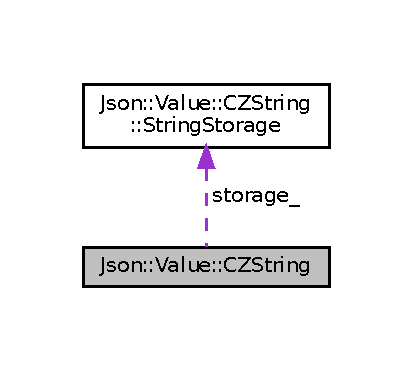
\includegraphics[width=198pt]{classJson_1_1Value_1_1CZString__coll__graph}
\end{center}
\end{figure}
\subsection*{Classes}
\begin{DoxyCompactItemize}
\item 
struct \hyperlink{structJson_1_1Value_1_1CZString_1_1StringStorage}{String\+Storage}
\end{DoxyCompactItemize}
\subsection*{Public Types}
\begin{DoxyCompactItemize}
\item 
\mbox{\Hypertarget{classJson_1_1Value_1_1CZString_a2805c46fb4a72bbaed55de6d75941b6d}\label{classJson_1_1Value_1_1CZString_a2805c46fb4a72bbaed55de6d75941b6d}} 
enum {\bfseries Duplication\+Policy} \{ {\bfseries no\+Duplication} = 0, 
{\bfseries duplicate}, 
{\bfseries duplicate\+On\+Copy}
 \}
\end{DoxyCompactItemize}
\subsection*{Public Member Functions}
\begin{DoxyCompactItemize}
\item 
\mbox{\Hypertarget{classJson_1_1Value_1_1CZString_a4b8aa6eaabdec78cffec96e088da996f}\label{classJson_1_1Value_1_1CZString_a4b8aa6eaabdec78cffec96e088da996f}} 
{\bfseries C\+Z\+String} (Array\+Index index)
\item 
\mbox{\Hypertarget{classJson_1_1Value_1_1CZString_a86a86eaf0cf26d4c861d0daa359d608a}\label{classJson_1_1Value_1_1CZString_a86a86eaf0cf26d4c861d0daa359d608a}} 
{\bfseries C\+Z\+String} (char const $\ast$str, unsigned length, Duplication\+Policy allocate)
\item 
\mbox{\Hypertarget{classJson_1_1Value_1_1CZString_a9685070d440335b55ef5c85747d25157}\label{classJson_1_1Value_1_1CZString_a9685070d440335b55ef5c85747d25157}} 
{\bfseries C\+Z\+String} (\hyperlink{classJson_1_1Value_1_1CZString}{C\+Z\+String} const \&other)
\item 
\mbox{\Hypertarget{classJson_1_1Value_1_1CZString_aba1b28d22cdd1eaad1c17f8844af9d4a}\label{classJson_1_1Value_1_1CZString_aba1b28d22cdd1eaad1c17f8844af9d4a}} 
\hyperlink{classJson_1_1Value_1_1CZString}{C\+Z\+String} \& {\bfseries operator=} (const \hyperlink{classJson_1_1Value_1_1CZString}{C\+Z\+String} \&other)
\item 
\mbox{\Hypertarget{classJson_1_1Value_1_1CZString_ae023bb91b4b4520c82d5e6e4da8c310a}\label{classJson_1_1Value_1_1CZString_ae023bb91b4b4520c82d5e6e4da8c310a}} 
bool {\bfseries operator$<$} (\hyperlink{classJson_1_1Value_1_1CZString}{C\+Z\+String} const \&other) const
\item 
\mbox{\Hypertarget{classJson_1_1Value_1_1CZString_ad41766c98fc6a6d5fcd72aaf78fc5db0}\label{classJson_1_1Value_1_1CZString_ad41766c98fc6a6d5fcd72aaf78fc5db0}} 
bool {\bfseries operator==} (\hyperlink{classJson_1_1Value_1_1CZString}{C\+Z\+String} const \&other) const
\item 
\mbox{\Hypertarget{classJson_1_1Value_1_1CZString_a0f3ba09401525d4f01dafd577122ee32}\label{classJson_1_1Value_1_1CZString_a0f3ba09401525d4f01dafd577122ee32}} 
Array\+Index {\bfseries index} () const
\item 
\mbox{\Hypertarget{classJson_1_1Value_1_1CZString_af6eee54f8dc43a1203d5af6ba0a5c9a2}\label{classJson_1_1Value_1_1CZString_af6eee54f8dc43a1203d5af6ba0a5c9a2}} 
char const  $\ast$ {\bfseries data} () const
\item 
\mbox{\Hypertarget{classJson_1_1Value_1_1CZString_aa7ee665d162c1f33b3ec818e289d8a5e}\label{classJson_1_1Value_1_1CZString_aa7ee665d162c1f33b3ec818e289d8a5e}} 
unsigned {\bfseries length} () const
\item 
\mbox{\Hypertarget{classJson_1_1Value_1_1CZString_a5991dfa2f6c2ba318373c7429fcd7a57}\label{classJson_1_1Value_1_1CZString_a5991dfa2f6c2ba318373c7429fcd7a57}} 
bool {\bfseries is\+Static\+String} () const
\end{DoxyCompactItemize}
\subsection*{Private Member Functions}
\begin{DoxyCompactItemize}
\item 
\mbox{\Hypertarget{classJson_1_1Value_1_1CZString_ad59f3542d2eea749a6a63409d1a02207}\label{classJson_1_1Value_1_1CZString_ad59f3542d2eea749a6a63409d1a02207}} 
void {\bfseries swap} (\hyperlink{classJson_1_1Value_1_1CZString}{C\+Z\+String} \&other)
\end{DoxyCompactItemize}
\subsection*{Private Attributes}
\begin{DoxyCompactItemize}
\item 
\mbox{\Hypertarget{classJson_1_1Value_1_1CZString_a5b4d28349294034d7f779c3c95d0306c}\label{classJson_1_1Value_1_1CZString_a5b4d28349294034d7f779c3c95d0306c}} 
char const  $\ast$ {\bfseries cstr\+\_\+}
\item 
\mbox{\Hypertarget{classJson_1_1Value_1_1CZString_a6f6b20ee7c8873fba58100f869ca2e5e}\label{classJson_1_1Value_1_1CZString_a6f6b20ee7c8873fba58100f869ca2e5e}} 
\begin{tabbing}
xx\=xx\=xx\=xx\=xx\=xx\=xx\=xx\=xx\=\kill
union \{\\
\>ArrayIndex {\bfseries index\_}\\
\>\hyperlink{structJson_1_1Value_1_1CZString_1_1StringStorage}{StringStorage} {\bfseries storage\_}\\
\}; \\

\end{tabbing}\end{DoxyCompactItemize}


The documentation for this class was generated from the following files\+:\begin{DoxyCompactItemize}
\item 
/home/mjonsson/repo/cpp\+Adv/media\+F\+W/inc/json/json.\+h\item 
/home/mjonsson/repo/cpp\+Adv/media\+F\+W/src/json/jsoncpp.\+cpp\end{DoxyCompactItemize}

\hypertarget{classDatabase}{}\section{Database Class Reference}
\label{classDatabase}\index{Database@{Database}}


Defines methods for database implementations.  




Inheritance diagram for Database\+:\nopagebreak
\begin{figure}[H]
\begin{center}
\leavevmode
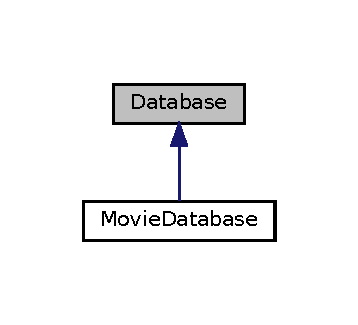
\includegraphics[width=270pt]{classDatabase__inherit__graph}
\end{center}
\end{figure}


Collaboration diagram for Database\+:\nopagebreak
\begin{figure}[H]
\begin{center}
\leavevmode
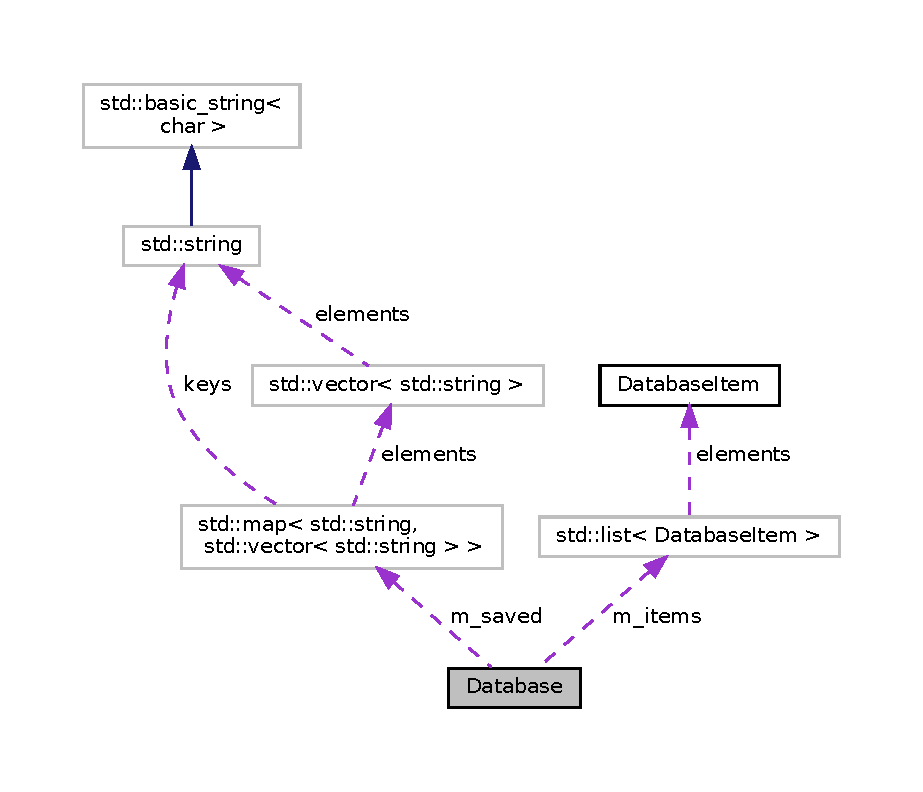
\includegraphics[width=350pt]{classDatabase__coll__graph}
\end{center}
\end{figure}
\subsection*{Public Member Functions}
\begin{DoxyCompactItemize}
\item 
\hyperlink{classDatabase_aa57fbada3001c2db58a0ca6c7071bd18}{Database} ()=default
\begin{DoxyCompactList}\small\item\em Default constructor. \end{DoxyCompactList}\item 
\hyperlink{classDatabase_a341cd0fe8c615e829e3a22b74c208bb5}{$\sim$\+Database} ()=default
\begin{DoxyCompactList}\small\item\em Default deconstructor. \end{DoxyCompactList}\item 
virtual void \hyperlink{classDatabase_a14d24487b4ea3b50097b9ac0f2b3f317}{sync\+Local\+Database} ()
\begin{DoxyCompactList}\small\item\em Sync info from json file and saves it to a list of database objects. \end{DoxyCompactList}\item 
virtual void \hyperlink{classDatabase_a80fa14ab9f4deadc9a2ab7493f1919a4}{push\+Item} (const \hyperlink{classDatabaseItem}{Database\+Item} \&m\+\_\+item)
\begin{DoxyCompactList}\small\item\em Uploads the requested database item. \end{DoxyCompactList}\item 
virtual \hyperlink{classDatabaseItem}{Database\+Item} \hyperlink{classDatabase_a40254eec69c7d7cc15da24a9f0b072b3}{fetch\+Item} (const std\+::string \&title)
\begin{DoxyCompactList}\small\item\em Fetch the requested database item. \end{DoxyCompactList}\item 
virtual void \hyperlink{classDatabase_a8f47437526eeec631f1328fab9bbbc75}{purge\+Item} (\hyperlink{classDatabaseItem}{Database\+Item} m\+\_\+item)
\begin{DoxyCompactList}\small\item\em Delete the requested database item. \end{DoxyCompactList}\item 
virtual void \hyperlink{classDatabase_afa345da530fd5c8dfe0c978917cd6049}{print\+All} ()
\begin{DoxyCompactList}\small\item\em Prints the entire database content. \end{DoxyCompactList}\item 
virtual long \hyperlink{classDatabase_a230225cb341eb23a99a83ef3d1abae53}{get\+Number\+Of\+Item} ()
\begin{DoxyCompactList}\small\item\em Method that return the size of the database. \end{DoxyCompactList}\end{DoxyCompactItemize}
\subsection*{Protected Attributes}
\begin{DoxyCompactItemize}
\item 
std\+::list$<$ \hyperlink{classDatabaseItem}{Database\+Item} $>$ \hyperlink{classDatabase_a5a4ac1f3bf0f5fd77a696174ad9e5c45}{m\+\_\+items}
\begin{DoxyCompactList}\small\item\em A protected list of Database\+Items. \end{DoxyCompactList}\item 
std\+::map$<$ std\+::string, std\+::vector$<$ std\+::string $>$ $>$ \hyperlink{classDatabase_a9f87cbe5a1be71d541083dffa8d8c9ad}{m\+\_\+saved}
\begin{DoxyCompactList}\small\item\em A protected vector of strings with info for the Database\+Items. \end{DoxyCompactList}\item 
std\+::mutex \hyperlink{classDatabase_a7f55f3a5d93c9694ee4f08a2f2135b1d}{m\+\_\+lock}
\begin{DoxyCompactList}\small\item\em A protected mutex for threadsafe r/w of Database\+Items. \end{DoxyCompactList}\item 
std\+::condition\+\_\+variable \hyperlink{classDatabase_a2ad8bf38964b3e18a0e168437acbdb27}{m\+\_\+empty\+List}
\begin{DoxyCompactList}\small\item\em A protected condittion variable for the mutex and \hyperlink{classDatabase}{Database} list. \end{DoxyCompactList}\end{DoxyCompactItemize}


\subsection{Detailed Description}
Defines methods for database implementations. 



\subsection{Constructor \& Destructor Documentation}
\mbox{\Hypertarget{classDatabase_aa57fbada3001c2db58a0ca6c7071bd18}\label{classDatabase_aa57fbada3001c2db58a0ca6c7071bd18}} 
\index{Database@{Database}!Database@{Database}}
\index{Database@{Database}!Database@{Database}}
\subsubsection{\texorpdfstring{Database()}{Database()}}
{\footnotesize\ttfamily Database\+::\+Database (\begin{DoxyParamCaption}{ }\end{DoxyParamCaption})\hspace{0.3cm}{\ttfamily [default]}}



Default constructor. 

\hyperlink{classDatabase_aa57fbada3001c2db58a0ca6c7071bd18}{Database()} \mbox{\Hypertarget{classDatabase_a341cd0fe8c615e829e3a22b74c208bb5}\label{classDatabase_a341cd0fe8c615e829e3a22b74c208bb5}} 
\index{Database@{Database}!````~Database@{$\sim$\+Database}}
\index{````~Database@{$\sim$\+Database}!Database@{Database}}
\subsubsection{\texorpdfstring{$\sim$\+Database()}{~Database()}}
{\footnotesize\ttfamily Database\+::$\sim$\+Database (\begin{DoxyParamCaption}{ }\end{DoxyParamCaption})\hspace{0.3cm}{\ttfamily [default]}}



Default deconstructor. 

\hyperlink{classDatabase_a341cd0fe8c615e829e3a22b74c208bb5}{$\sim$\+Database()} 

\subsection{Member Function Documentation}
\mbox{\Hypertarget{classDatabase_a40254eec69c7d7cc15da24a9f0b072b3}\label{classDatabase_a40254eec69c7d7cc15da24a9f0b072b3}} 
\index{Database@{Database}!fetch\+Item@{fetch\+Item}}
\index{fetch\+Item@{fetch\+Item}!Database@{Database}}
\subsubsection{\texorpdfstring{fetch\+Item()}{fetchItem()}}
{\footnotesize\ttfamily virtual \hyperlink{classDatabaseItem}{Database\+Item} Database\+::fetch\+Item (\begin{DoxyParamCaption}\item[{const std\+::string \&}]{title }\end{DoxyParamCaption})\hspace{0.3cm}{\ttfamily [inline]}, {\ttfamily [virtual]}}



Fetch the requested database item. 

A const reference to a title

\begin{DoxyReturn}{Returns}
The requested \hyperlink{classDatabaseItem}{Database\+Item}
\end{DoxyReturn}


Reimplemented in \hyperlink{classMovieDatabase_ac0bb39b8be599ffea76081809ae42dda}{Movie\+Database}, and \hyperlink{classSeriesDatabase_af5303a723910395b31f2e01088de9130}{Series\+Database}.

\mbox{\Hypertarget{classDatabase_a230225cb341eb23a99a83ef3d1abae53}\label{classDatabase_a230225cb341eb23a99a83ef3d1abae53}} 
\index{Database@{Database}!get\+Number\+Of\+Item@{get\+Number\+Of\+Item}}
\index{get\+Number\+Of\+Item@{get\+Number\+Of\+Item}!Database@{Database}}
\subsubsection{\texorpdfstring{get\+Number\+Of\+Item()}{getNumberOfItem()}}
{\footnotesize\ttfamily virtual long Database\+::get\+Number\+Of\+Item (\begin{DoxyParamCaption}{ }\end{DoxyParamCaption})\hspace{0.3cm}{\ttfamily [inline]}, {\ttfamily [virtual]}}



Method that return the size of the database. 

\begin{DoxyReturn}{Returns}
Size of the database (long).
\end{DoxyReturn}


Reimplemented in \hyperlink{classMovieDatabase_a9a386f51dd72d63414a124cbcfcd879b}{Movie\+Database}, and \hyperlink{classSeriesDatabase_af5fe5a423303eff4489a7679907ef994}{Series\+Database}.

\mbox{\Hypertarget{classDatabase_afa345da530fd5c8dfe0c978917cd6049}\label{classDatabase_afa345da530fd5c8dfe0c978917cd6049}} 
\index{Database@{Database}!print\+All@{print\+All}}
\index{print\+All@{print\+All}!Database@{Database}}
\subsubsection{\texorpdfstring{print\+All()}{printAll()}}
{\footnotesize\ttfamily virtual void Database\+::print\+All (\begin{DoxyParamCaption}{ }\end{DoxyParamCaption})\hspace{0.3cm}{\ttfamily [inline]}, {\ttfamily [virtual]}}



Prints the entire database content. 

s 

Reimplemented in \hyperlink{classMovieDatabase_af1e13b6fc0fd7186e98edbe2cf187618}{Movie\+Database}, and \hyperlink{classSeriesDatabase_ae2bf5323216e0043292494d3f0ac978c}{Series\+Database}.

\mbox{\Hypertarget{classDatabase_a8f47437526eeec631f1328fab9bbbc75}\label{classDatabase_a8f47437526eeec631f1328fab9bbbc75}} 
\index{Database@{Database}!purge\+Item@{purge\+Item}}
\index{purge\+Item@{purge\+Item}!Database@{Database}}
\subsubsection{\texorpdfstring{purge\+Item()}{purgeItem()}}
{\footnotesize\ttfamily virtual void Database\+::purge\+Item (\begin{DoxyParamCaption}\item[{\hyperlink{classDatabaseItem}{Database\+Item}}]{m\+\_\+item }\end{DoxyParamCaption})\hspace{0.3cm}{\ttfamily [inline]}, {\ttfamily [virtual]}}



Delete the requested database item. 

A const reference to a database item

Reimplemented in \hyperlink{classMovieDatabase_ad3ce59d0fa7f64937085e7504bd3b85a}{Movie\+Database}, and \hyperlink{classSeriesDatabase_a863a35987b5a4de15a121b8b4358e353}{Series\+Database}.

\mbox{\Hypertarget{classDatabase_a80fa14ab9f4deadc9a2ab7493f1919a4}\label{classDatabase_a80fa14ab9f4deadc9a2ab7493f1919a4}} 
\index{Database@{Database}!push\+Item@{push\+Item}}
\index{push\+Item@{push\+Item}!Database@{Database}}
\subsubsection{\texorpdfstring{push\+Item()}{pushItem()}}
{\footnotesize\ttfamily virtual void Database\+::push\+Item (\begin{DoxyParamCaption}\item[{const \hyperlink{classDatabaseItem}{Database\+Item} \&}]{m\+\_\+item }\end{DoxyParamCaption})\hspace{0.3cm}{\ttfamily [inline]}, {\ttfamily [virtual]}}



Uploads the requested database item. 

A const reference to a database item

Reimplemented in \hyperlink{classMovieDatabase_a203b9b5c1b325997ce519859a436b6ce}{Movie\+Database}, and \hyperlink{classSeriesDatabase_a7591f89ab256d9f5a41235f5552e4e23}{Series\+Database}.

\mbox{\Hypertarget{classDatabase_a14d24487b4ea3b50097b9ac0f2b3f317}\label{classDatabase_a14d24487b4ea3b50097b9ac0f2b3f317}} 
\index{Database@{Database}!sync\+Local\+Database@{sync\+Local\+Database}}
\index{sync\+Local\+Database@{sync\+Local\+Database}!Database@{Database}}
\subsubsection{\texorpdfstring{sync\+Local\+Database()}{syncLocalDatabase()}}
{\footnotesize\ttfamily virtual void Database\+::sync\+Local\+Database (\begin{DoxyParamCaption}{ }\end{DoxyParamCaption})\hspace{0.3cm}{\ttfamily [inline]}, {\ttfamily [virtual]}}



Sync info from json file and saves it to a list of database objects. 

Database\+::sync\+Database() 

Reimplemented in \hyperlink{classMovieDatabase_aee175db6a2a357b6180fcab5d57eddd5}{Movie\+Database}, and \hyperlink{classSeriesDatabase_a0ba159b6d52a3cfa07135c7d8b37ef76}{Series\+Database}.



\subsection{Member Data Documentation}
\mbox{\Hypertarget{classDatabase_a2ad8bf38964b3e18a0e168437acbdb27}\label{classDatabase_a2ad8bf38964b3e18a0e168437acbdb27}} 
\index{Database@{Database}!m\+\_\+empty\+List@{m\+\_\+empty\+List}}
\index{m\+\_\+empty\+List@{m\+\_\+empty\+List}!Database@{Database}}
\subsubsection{\texorpdfstring{m\+\_\+empty\+List}{m\_emptyList}}
{\footnotesize\ttfamily std\+::condition\+\_\+variable Database\+::m\+\_\+empty\+List\hspace{0.3cm}{\ttfamily [protected]}}



A protected condittion variable for the mutex and \hyperlink{classDatabase}{Database} list. 

\mbox{\Hypertarget{classDatabase_a5a4ac1f3bf0f5fd77a696174ad9e5c45}\label{classDatabase_a5a4ac1f3bf0f5fd77a696174ad9e5c45}} 
\index{Database@{Database}!m\+\_\+items@{m\+\_\+items}}
\index{m\+\_\+items@{m\+\_\+items}!Database@{Database}}
\subsubsection{\texorpdfstring{m\+\_\+items}{m\_items}}
{\footnotesize\ttfamily std\+::list$<$\hyperlink{classDatabaseItem}{Database\+Item}$>$ Database\+::m\+\_\+items\hspace{0.3cm}{\ttfamily [protected]}}



A protected list of Database\+Items. 

\mbox{\Hypertarget{classDatabase_a7f55f3a5d93c9694ee4f08a2f2135b1d}\label{classDatabase_a7f55f3a5d93c9694ee4f08a2f2135b1d}} 
\index{Database@{Database}!m\+\_\+lock@{m\+\_\+lock}}
\index{m\+\_\+lock@{m\+\_\+lock}!Database@{Database}}
\subsubsection{\texorpdfstring{m\+\_\+lock}{m\_lock}}
{\footnotesize\ttfamily std\+::mutex Database\+::m\+\_\+lock\hspace{0.3cm}{\ttfamily [mutable]}, {\ttfamily [protected]}}



A protected mutex for threadsafe r/w of Database\+Items. 

\mbox{\Hypertarget{classDatabase_a9f87cbe5a1be71d541083dffa8d8c9ad}\label{classDatabase_a9f87cbe5a1be71d541083dffa8d8c9ad}} 
\index{Database@{Database}!m\+\_\+saved@{m\+\_\+saved}}
\index{m\+\_\+saved@{m\+\_\+saved}!Database@{Database}}
\subsubsection{\texorpdfstring{m\+\_\+saved}{m\_saved}}
{\footnotesize\ttfamily std\+::map$<$std\+::string, std\+::vector$<$std\+::string$>$ $>$ Database\+::m\+\_\+saved\hspace{0.3cm}{\ttfamily [protected]}}



A protected vector of strings with info for the Database\+Items. 



The documentation for this class was generated from the following file\+:\begin{DoxyCompactItemize}
\item 
inc/database/Database.\+h\end{DoxyCompactItemize}

\hypertarget{classDatabaseItem}{}\section{Database\+Item Class Reference}
\label{classDatabaseItem}\index{Database\+Item@{Database\+Item}}


Collaboration diagram for Database\+Item\+:
\nopagebreak
\begin{figure}[H]
\begin{center}
\leavevmode
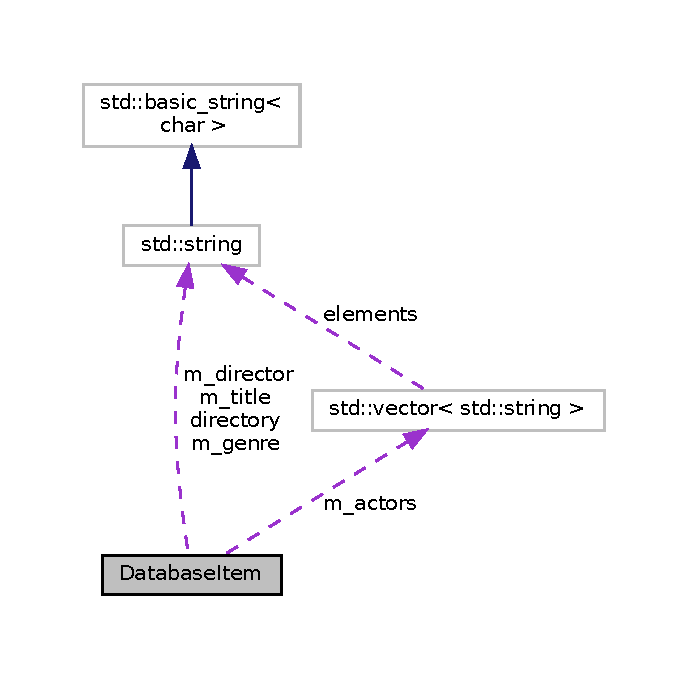
\includegraphics[width=330pt]{classDatabaseItem__coll__graph}
\end{center}
\end{figure}
\subsection*{Public Member Functions}
\begin{DoxyCompactItemize}
\item 
\mbox{\Hypertarget{classDatabaseItem_abb8e57f5ec53e855c541e5b27c4dfe10}\label{classDatabaseItem_abb8e57f5ec53e855c541e5b27c4dfe10}} 
{\bfseries Database\+Item} (std\+::vector$<$ std\+::string $>$ \+\_\+actors, std\+::string \+\_\+title, std\+::string \+\_\+genre, std\+::string \+\_\+director)
\item 
\mbox{\Hypertarget{classDatabaseItem_a51f4dbeb282806b7ac10e6b49b90eeef}\label{classDatabaseItem_a51f4dbeb282806b7ac10e6b49b90eeef}} 
void {\bfseries set\+Feature} (\hyperlink{structTags}{Tags} feature)
\item 
\mbox{\Hypertarget{classDatabaseItem_a98560961c4ab1266fe9b10f094bea568}\label{classDatabaseItem_a98560961c4ab1266fe9b10f094bea568}} 
std\+::vector$<$ std\+::string $>$ {\bfseries get\+Actors} ()
\item 
\mbox{\Hypertarget{classDatabaseItem_a87f2ebf677aaec4bc2e95eea2b7bd329}\label{classDatabaseItem_a87f2ebf677aaec4bc2e95eea2b7bd329}} 
std\+::string {\bfseries get\+Title} () const
\item 
\mbox{\Hypertarget{classDatabaseItem_a7edc61bf54ac2e48e921b9948d9efecb}\label{classDatabaseItem_a7edc61bf54ac2e48e921b9948d9efecb}} 
std\+::string {\bfseries get\+Director} ()
\item 
\mbox{\Hypertarget{classDatabaseItem_ac1d9f64c889ed271aa0f586a62a2c82a}\label{classDatabaseItem_ac1d9f64c889ed271aa0f586a62a2c82a}} 
std\+::string {\bfseries get\+Genre} ()
\item 
\mbox{\Hypertarget{classDatabaseItem_afcca0a554ac65bdcf796480e8d2920f4}\label{classDatabaseItem_afcca0a554ac65bdcf796480e8d2920f4}} 
std\+::string {\bfseries get\+Dir} ()
\end{DoxyCompactItemize}
\subsection*{Private Attributes}
\begin{DoxyCompactItemize}
\item 
\mbox{\Hypertarget{classDatabaseItem_a5ecbf8e196e110a738bb8ab1fbdff80b}\label{classDatabaseItem_a5ecbf8e196e110a738bb8ab1fbdff80b}} 
std\+::string {\bfseries directory}
\item 
\mbox{\Hypertarget{classDatabaseItem_aae3a4413ab461a85af2e79c0491a4e51}\label{classDatabaseItem_aae3a4413ab461a85af2e79c0491a4e51}} 
std\+::string {\bfseries m\+\_\+title}
\item 
\mbox{\Hypertarget{classDatabaseItem_a31482f012b886663cd8f2374e5bfe715}\label{classDatabaseItem_a31482f012b886663cd8f2374e5bfe715}} 
std\+::string {\bfseries m\+\_\+genre}
\item 
\mbox{\Hypertarget{classDatabaseItem_ad83b8f7fe4c6de1a3440ee3397192b01}\label{classDatabaseItem_ad83b8f7fe4c6de1a3440ee3397192b01}} 
std\+::string {\bfseries m\+\_\+director}
\item 
\mbox{\Hypertarget{classDatabaseItem_af98cce4f0865b2bf17d6a484c17ffaf9}\label{classDatabaseItem_af98cce4f0865b2bf17d6a484c17ffaf9}} 
std\+::vector$<$ std\+::string $>$ {\bfseries m\+\_\+actors}
\end{DoxyCompactItemize}


The documentation for this class was generated from the following file\+:\begin{DoxyCompactItemize}
\item 
/home/mjonsson/repo/cpp\+Adv/media\+F\+W/inc/\+Database/Database\+Item.\+h\end{DoxyCompactItemize}

\hypertarget{classJson_1_1OurReader_1_1ErrorInfo}{}\section{Json\+:\+:Our\+Reader\+:\+:Error\+Info Class Reference}
\label{classJson_1_1OurReader_1_1ErrorInfo}\index{Json\+::\+Our\+Reader\+::\+Error\+Info@{Json\+::\+Our\+Reader\+::\+Error\+Info}}


Collaboration diagram for Json\+:\+:Our\+Reader\+:\+:Error\+Info\+:
\nopagebreak
\begin{figure}[H]
\begin{center}
\leavevmode
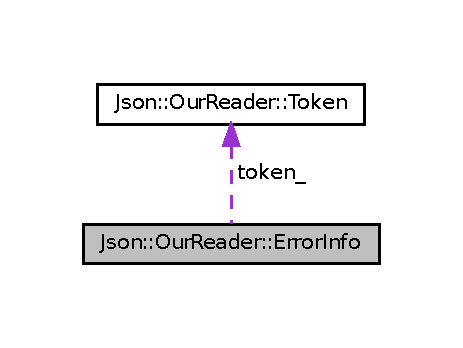
\includegraphics[width=222pt]{classJson_1_1OurReader_1_1ErrorInfo__coll__graph}
\end{center}
\end{figure}
\subsection*{Public Attributes}
\begin{DoxyCompactItemize}
\item 
\mbox{\Hypertarget{classJson_1_1OurReader_1_1ErrorInfo_ad05204ecabe5e7201a842935b874ae9a}\label{classJson_1_1OurReader_1_1ErrorInfo_ad05204ecabe5e7201a842935b874ae9a}} 
\hyperlink{classJson_1_1OurReader_1_1Token}{Token} {\bfseries token\+\_\+}
\item 
\mbox{\Hypertarget{classJson_1_1OurReader_1_1ErrorInfo_af14b6bf58ee1cb3388c18ee336ee2394}\label{classJson_1_1OurReader_1_1ErrorInfo_af14b6bf58ee1cb3388c18ee336ee2394}} 
J\+S\+O\+N\+C\+P\+P\+\_\+\+S\+T\+R\+I\+NG {\bfseries message\+\_\+}
\item 
\mbox{\Hypertarget{classJson_1_1OurReader_1_1ErrorInfo_a77ba2d32a471c7b9bc14621b76a5bdab}\label{classJson_1_1OurReader_1_1ErrorInfo_a77ba2d32a471c7b9bc14621b76a5bdab}} 
Location {\bfseries extra\+\_\+}
\end{DoxyCompactItemize}


The documentation for this class was generated from the following file\+:\begin{DoxyCompactItemize}
\item 
/home/mjonsson/repo/cpp\+Adv/media\+F\+W/src/json/jsoncpp.\+cpp\end{DoxyCompactItemize}

\hypertarget{classJson_1_1Reader_1_1ErrorInfo}{}\section{Json\+:\+:Reader\+:\+:Error\+Info Class Reference}
\label{classJson_1_1Reader_1_1ErrorInfo}\index{Json\+::\+Reader\+::\+Error\+Info@{Json\+::\+Reader\+::\+Error\+Info}}


Collaboration diagram for Json\+:\+:Reader\+:\+:Error\+Info\+:
\nopagebreak
\begin{figure}[H]
\begin{center}
\leavevmode
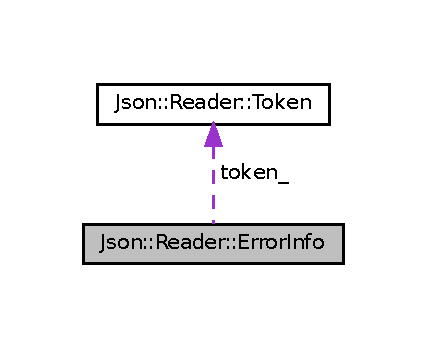
\includegraphics[width=205pt]{classJson_1_1Reader_1_1ErrorInfo__coll__graph}
\end{center}
\end{figure}
\subsection*{Public Attributes}
\begin{DoxyCompactItemize}
\item 
\mbox{\Hypertarget{classJson_1_1Reader_1_1ErrorInfo_a52e1c71b12eb1c3f0395d7ef1e778ce6}\label{classJson_1_1Reader_1_1ErrorInfo_a52e1c71b12eb1c3f0395d7ef1e778ce6}} 
\hyperlink{classJson_1_1Reader_1_1Token}{Token} {\bfseries token\+\_\+}
\item 
\mbox{\Hypertarget{classJson_1_1Reader_1_1ErrorInfo_a3529d420f7c83165565bf294a5d6ed13}\label{classJson_1_1Reader_1_1ErrorInfo_a3529d420f7c83165565bf294a5d6ed13}} 
J\+S\+O\+N\+C\+P\+P\+\_\+\+S\+T\+R\+I\+NG {\bfseries message\+\_\+}
\item 
\mbox{\Hypertarget{classJson_1_1Reader_1_1ErrorInfo_af92c24acf642b040d6e40aac4952d44d}\label{classJson_1_1Reader_1_1ErrorInfo_af92c24acf642b040d6e40aac4952d44d}} 
Location {\bfseries extra\+\_\+}
\end{DoxyCompactItemize}


The documentation for this class was generated from the following file\+:\begin{DoxyCompactItemize}
\item 
/home/mjonsson/repo/cpp\+Adv/media\+F\+W/inc/json/json.\+h\end{DoxyCompactItemize}

\hypertarget{classJson_1_1Exception}{}\section{Json\+:\+:Exception Class Reference}
\label{classJson_1_1Exception}\index{Json\+::\+Exception@{Json\+::\+Exception}}


{\ttfamily \#include $<$json.\+h$>$}



Inheritance diagram for Json\+:\+:Exception\+:
\nopagebreak
\begin{figure}[H]
\begin{center}
\leavevmode
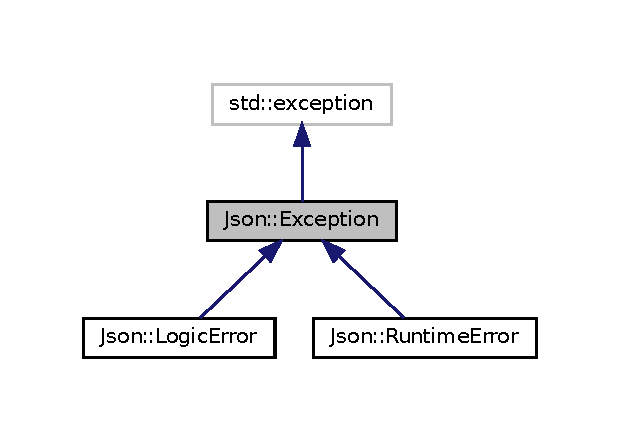
\includegraphics[width=298pt]{classJson_1_1Exception__inherit__graph}
\end{center}
\end{figure}


Collaboration diagram for Json\+:\+:Exception\+:
\nopagebreak
\begin{figure}[H]
\begin{center}
\leavevmode
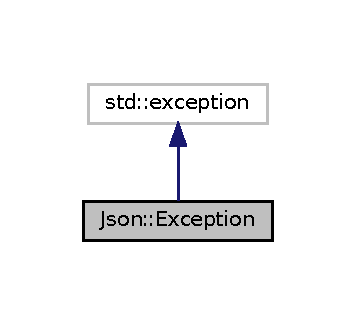
\includegraphics[width=171pt]{classJson_1_1Exception__coll__graph}
\end{center}
\end{figure}
\subsection*{Public Member Functions}
\begin{DoxyCompactItemize}
\item 
\mbox{\Hypertarget{classJson_1_1Exception_ae764aa42e0755bd4ce9d303e2733fa8f}\label{classJson_1_1Exception_ae764aa42e0755bd4ce9d303e2733fa8f}} 
{\bfseries Exception} (J\+S\+O\+N\+C\+P\+P\+\_\+\+S\+T\+R\+I\+NG const \&msg)
\item 
\mbox{\Hypertarget{classJson_1_1Exception_a70b7ce35e761fb93e8cd338e04619cd6}\label{classJson_1_1Exception_a70b7ce35e761fb93e8cd338e04619cd6}} 
char const  $\ast$ {\bfseries what} () const J\+S\+O\+N\+C\+P\+P\+\_\+\+N\+O\+E\+X\+C\+E\+PT J\+S\+O\+N\+C\+P\+P\+\_\+\+O\+V\+E\+R\+R\+I\+DE
\end{DoxyCompactItemize}
\subsection*{Protected Attributes}
\begin{DoxyCompactItemize}
\item 
\mbox{\Hypertarget{classJson_1_1Exception_aae3cbb8b45bf21480f64502a8329659f}\label{classJson_1_1Exception_aae3cbb8b45bf21480f64502a8329659f}} 
J\+S\+O\+N\+C\+P\+P\+\_\+\+S\+T\+R\+I\+NG {\bfseries msg\+\_\+}
\end{DoxyCompactItemize}


\subsection{Detailed Description}
Base class for all exceptions we throw.

We use nothing but these internally. Of course, S\+TL can throw others. 

The documentation for this class was generated from the following files\+:\begin{DoxyCompactItemize}
\item 
/home/mjonsson/repo/cpp\+Adv/media\+F\+W/inc/json/json.\+h\item 
/home/mjonsson/repo/cpp\+Adv/media\+F\+W/src/json/jsoncpp.\+cpp\end{DoxyCompactItemize}

\hypertarget{classJson_1_1CharReader_1_1Factory}{}\section{Json\+:\+:Char\+Reader\+:\+:Factory Class Reference}
\label{classJson_1_1CharReader_1_1Factory}\index{Json\+::\+Char\+Reader\+::\+Factory@{Json\+::\+Char\+Reader\+::\+Factory}}


Inheritance diagram for Json\+:\+:Char\+Reader\+:\+:Factory\+:
\nopagebreak
\begin{figure}[H]
\begin{center}
\leavevmode
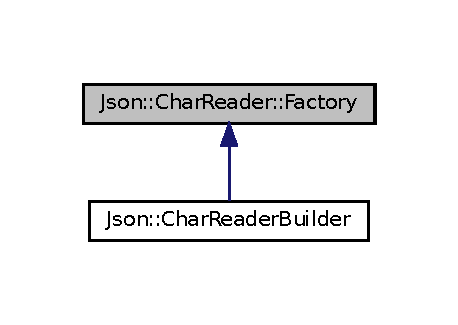
\includegraphics[width=220pt]{classJson_1_1CharReader_1_1Factory__inherit__graph}
\end{center}
\end{figure}
\subsection*{Public Member Functions}
\begin{DoxyCompactItemize}
\item 
virtual \hyperlink{classJson_1_1CharReader}{Char\+Reader} $\ast$ \hyperlink{classJson_1_1CharReader_1_1Factory_a4c5862a1ffd432372dbe65cf59de98c4}{new\+Char\+Reader} () const =0
\begin{DoxyCompactList}\small\item\em Allocate a \hyperlink{classJson_1_1CharReader}{Char\+Reader} via operator new(). \end{DoxyCompactList}\end{DoxyCompactItemize}


\subsection{Member Function Documentation}
\mbox{\Hypertarget{classJson_1_1CharReader_1_1Factory_a4c5862a1ffd432372dbe65cf59de98c4}\label{classJson_1_1CharReader_1_1Factory_a4c5862a1ffd432372dbe65cf59de98c4}} 
\index{Json\+::\+Char\+Reader\+::\+Factory@{Json\+::\+Char\+Reader\+::\+Factory}!new\+Char\+Reader@{new\+Char\+Reader}}
\index{new\+Char\+Reader@{new\+Char\+Reader}!Json\+::\+Char\+Reader\+::\+Factory@{Json\+::\+Char\+Reader\+::\+Factory}}
\subsubsection{\texorpdfstring{new\+Char\+Reader()}{newCharReader()}}
{\footnotesize\ttfamily virtual \hyperlink{classJson_1_1CharReader}{Char\+Reader}$\ast$ Json\+::\+Char\+Reader\+::\+Factory\+::new\+Char\+Reader (\begin{DoxyParamCaption}{ }\end{DoxyParamCaption}) const\hspace{0.3cm}{\ttfamily [pure virtual]}}



Allocate a \hyperlink{classJson_1_1CharReader}{Char\+Reader} via operator new(). 


\begin{DoxyExceptions}{Exceptions}
{\em std\+::exception} & if something goes wrong (e.\+g. invalid settings) \\
\hline
\end{DoxyExceptions}


Implemented in \hyperlink{classJson_1_1CharReaderBuilder_a3a262fcc76c1eb8eebfd4718fb4e9722}{Json\+::\+Char\+Reader\+Builder}.



The documentation for this class was generated from the following file\+:\begin{DoxyCompactItemize}
\item 
/home/mjonsson/repo/cpp\+Adv/media\+F\+W/inc/json/json.\+h\end{DoxyCompactItemize}

\hypertarget{classJson_1_1StreamWriter_1_1Factory}{}\section{Json\+:\+:Stream\+Writer\+:\+:Factory Class Reference}
\label{classJson_1_1StreamWriter_1_1Factory}\index{Json\+::\+Stream\+Writer\+::\+Factory@{Json\+::\+Stream\+Writer\+::\+Factory}}


A simple abstract factory.  




{\ttfamily \#include $<$json.\+h$>$}



Inheritance diagram for Json\+:\+:Stream\+Writer\+:\+:Factory\+:
\nopagebreak
\begin{figure}[H]
\begin{center}
\leavevmode
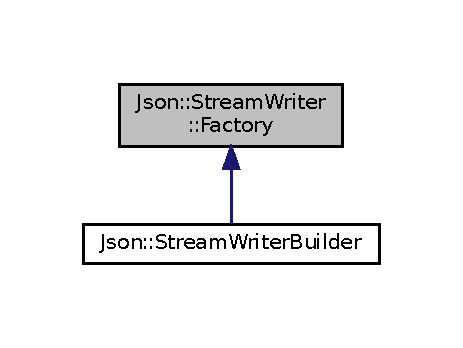
\includegraphics[width=222pt]{classJson_1_1StreamWriter_1_1Factory__inherit__graph}
\end{center}
\end{figure}
\subsection*{Public Member Functions}
\begin{DoxyCompactItemize}
\item 
virtual \hyperlink{classJson_1_1StreamWriter}{Stream\+Writer} $\ast$ \hyperlink{classJson_1_1StreamWriter_1_1Factory_a9d30ec53e8288cd53befccf1009c5f31}{new\+Stream\+Writer} () const =0
\begin{DoxyCompactList}\small\item\em Allocate a \hyperlink{classJson_1_1CharReader}{Char\+Reader} via operator new(). \end{DoxyCompactList}\end{DoxyCompactItemize}


\subsection{Detailed Description}
A simple abstract factory. 

\subsection{Member Function Documentation}
\mbox{\Hypertarget{classJson_1_1StreamWriter_1_1Factory_a9d30ec53e8288cd53befccf1009c5f31}\label{classJson_1_1StreamWriter_1_1Factory_a9d30ec53e8288cd53befccf1009c5f31}} 
\index{Json\+::\+Stream\+Writer\+::\+Factory@{Json\+::\+Stream\+Writer\+::\+Factory}!new\+Stream\+Writer@{new\+Stream\+Writer}}
\index{new\+Stream\+Writer@{new\+Stream\+Writer}!Json\+::\+Stream\+Writer\+::\+Factory@{Json\+::\+Stream\+Writer\+::\+Factory}}
\subsubsection{\texorpdfstring{new\+Stream\+Writer()}{newStreamWriter()}}
{\footnotesize\ttfamily virtual \hyperlink{classJson_1_1StreamWriter}{Stream\+Writer}$\ast$ Json\+::\+Stream\+Writer\+::\+Factory\+::new\+Stream\+Writer (\begin{DoxyParamCaption}{ }\end{DoxyParamCaption}) const\hspace{0.3cm}{\ttfamily [pure virtual]}}



Allocate a \hyperlink{classJson_1_1CharReader}{Char\+Reader} via operator new(). 


\begin{DoxyExceptions}{Exceptions}
{\em std\+::exception} & if something goes wrong (e.\+g. invalid settings) \\
\hline
\end{DoxyExceptions}


Implemented in \hyperlink{classJson_1_1StreamWriterBuilder_ab9ee278609f88ae04a7c1a84e1f559e6}{Json\+::\+Stream\+Writer\+Builder}.



The documentation for this class was generated from the following files\+:\begin{DoxyCompactItemize}
\item 
/home/mjonsson/repo/cpp\+Adv/media\+F\+W/inc/json/json.\+h\item 
/home/mjonsson/repo/cpp\+Adv/media\+F\+W/src/json/jsoncpp.\+cpp\end{DoxyCompactItemize}

\hypertarget{classJson_1_1Features}{}\section{Json\+:\+:Features Class Reference}
\label{classJson_1_1Features}\index{Json\+::\+Features@{Json\+::\+Features}}


Configuration passed to reader and writer. This configuration object can be used to force the \hyperlink{classJson_1_1Reader}{Reader} or Writer to behave in a standard conforming way.  




{\ttfamily \#include $<$json.\+h$>$}

\subsection*{Public Member Functions}
\begin{DoxyCompactItemize}
\item 
\mbox{\Hypertarget{classJson_1_1Features_ad15a091cb61bb31323299a95970d2644}\label{classJson_1_1Features_ad15a091cb61bb31323299a95970d2644}} 
\hyperlink{classJson_1_1Features_ad15a091cb61bb31323299a95970d2644}{Features} ()
\begin{DoxyCompactList}\small\item\em Initialize the configuration like Json\+Config\+::all\+Features;. \end{DoxyCompactList}\end{DoxyCompactItemize}
\subsection*{Static Public Member Functions}
\begin{DoxyCompactItemize}
\item 
static \hyperlink{classJson_1_1Features}{Features} \hyperlink{classJson_1_1Features_a63894da6e2c100b38741fa933f3d33ae}{all} ()
\begin{DoxyCompactList}\small\item\em A configuration that allows all features and assumes all strings are U\+T\+F-\/8. \end{DoxyCompactList}\item 
static \hyperlink{classJson_1_1Features}{Features} \hyperlink{classJson_1_1Features_ae23176c14b2e79e81fb61fb1a8ab58ee}{strict\+Mode} ()
\begin{DoxyCompactList}\small\item\em A configuration that is strictly compatible with the J\+S\+ON specification. \end{DoxyCompactList}\end{DoxyCompactItemize}
\subsection*{Public Attributes}
\begin{DoxyCompactItemize}
\item 
\mbox{\Hypertarget{classJson_1_1Features_a33afd389719624b6bdb23950b3c346c9}\label{classJson_1_1Features_a33afd389719624b6bdb23950b3c346c9}} 
bool \hyperlink{classJson_1_1Features_a33afd389719624b6bdb23950b3c346c9}{allow\+Comments\+\_\+}
\begin{DoxyCompactList}\small\item\em {\ttfamily true} if comments are allowed. Default\+: {\ttfamily true}. \end{DoxyCompactList}\item 
bool \hyperlink{classJson_1_1Features_a1162c37a1458adc32582b585b552f9c3}{strict\+Root\+\_\+}
\item 
\mbox{\Hypertarget{classJson_1_1Features_a5076aa72c05c7596ac339ede36c97a6a}\label{classJson_1_1Features_a5076aa72c05c7596ac339ede36c97a6a}} 
bool \hyperlink{classJson_1_1Features_a5076aa72c05c7596ac339ede36c97a6a}{allow\+Dropped\+Null\+Placeholders\+\_\+}
\begin{DoxyCompactList}\small\item\em {\ttfamily true} if dropped null placeholders are allowed. Default\+: {\ttfamily false}. \end{DoxyCompactList}\item 
\mbox{\Hypertarget{classJson_1_1Features_aff3cb16b79d15d3d761b11a0dd6d4d6b}\label{classJson_1_1Features_aff3cb16b79d15d3d761b11a0dd6d4d6b}} 
bool \hyperlink{classJson_1_1Features_aff3cb16b79d15d3d761b11a0dd6d4d6b}{allow\+Numeric\+Keys\+\_\+}
\begin{DoxyCompactList}\small\item\em {\ttfamily true} if numeric object key are allowed. Default\+: {\ttfamily false}. \end{DoxyCompactList}\end{DoxyCompactItemize}


\subsection{Detailed Description}
Configuration passed to reader and writer. This configuration object can be used to force the \hyperlink{classJson_1_1Reader}{Reader} or Writer to behave in a standard conforming way. 

\subsection{Member Function Documentation}
\mbox{\Hypertarget{classJson_1_1Features_a63894da6e2c100b38741fa933f3d33ae}\label{classJson_1_1Features_a63894da6e2c100b38741fa933f3d33ae}} 
\index{Json\+::\+Features@{Json\+::\+Features}!all@{all}}
\index{all@{all}!Json\+::\+Features@{Json\+::\+Features}}
\subsubsection{\texorpdfstring{all()}{all()}}
{\footnotesize\ttfamily \hyperlink{classJson_1_1Features}{Features} Json\+::\+Features\+::all (\begin{DoxyParamCaption}{ }\end{DoxyParamCaption})\hspace{0.3cm}{\ttfamily [static]}}



A configuration that allows all features and assumes all strings are U\+T\+F-\/8. 


\begin{DoxyItemize}
\item C \& C++ comments are allowed
\item Root object can be any J\+S\+ON value
\item Assumes \hyperlink{classJson_1_1Value}{Value} strings are encoded in U\+T\+F-\/8 
\end{DoxyItemize}\mbox{\Hypertarget{classJson_1_1Features_ae23176c14b2e79e81fb61fb1a8ab58ee}\label{classJson_1_1Features_ae23176c14b2e79e81fb61fb1a8ab58ee}} 
\index{Json\+::\+Features@{Json\+::\+Features}!strict\+Mode@{strict\+Mode}}
\index{strict\+Mode@{strict\+Mode}!Json\+::\+Features@{Json\+::\+Features}}
\subsubsection{\texorpdfstring{strict\+Mode()}{strictMode()}}
{\footnotesize\ttfamily \hyperlink{classJson_1_1Features}{Features} Json\+::\+Features\+::strict\+Mode (\begin{DoxyParamCaption}{ }\end{DoxyParamCaption})\hspace{0.3cm}{\ttfamily [static]}}



A configuration that is strictly compatible with the J\+S\+ON specification. 


\begin{DoxyItemize}
\item Comments are forbidden.
\item Root object must be either an array or an object value.
\item Assumes \hyperlink{classJson_1_1Value}{Value} strings are encoded in U\+T\+F-\/8 
\end{DoxyItemize}

\subsection{Member Data Documentation}
\mbox{\Hypertarget{classJson_1_1Features_a1162c37a1458adc32582b585b552f9c3}\label{classJson_1_1Features_a1162c37a1458adc32582b585b552f9c3}} 
\index{Json\+::\+Features@{Json\+::\+Features}!strict\+Root\+\_\+@{strict\+Root\+\_\+}}
\index{strict\+Root\+\_\+@{strict\+Root\+\_\+}!Json\+::\+Features@{Json\+::\+Features}}
\subsubsection{\texorpdfstring{strict\+Root\+\_\+}{strictRoot\_}}
{\footnotesize\ttfamily bool Json\+::\+Features\+::strict\+Root\+\_\+}

{\ttfamily true} if root must be either an array or an object value. Default\+: {\ttfamily false}. 

The documentation for this class was generated from the following files\+:\begin{DoxyCompactItemize}
\item 
/home/mjonsson/repo/cpp\+Adv/media\+F\+W/inc/json/json.\+h\item 
/home/mjonsson/repo/cpp\+Adv/media\+F\+W/src/json/jsoncpp.\+cpp\end{DoxyCompactItemize}

\hypertarget{classJsonParser}{}\section{Json\+Parser Class Reference}
\label{classJsonParser}\index{Json\+Parser@{Json\+Parser}}


Inheritance diagram for Json\+Parser\+:\nopagebreak
\begin{figure}[H]
\begin{center}
\leavevmode
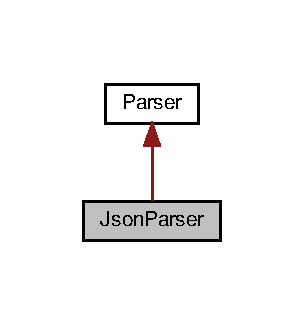
\includegraphics[width=146pt]{classJsonParser__inherit__graph}
\end{center}
\end{figure}


Collaboration diagram for Json\+Parser\+:\nopagebreak
\begin{figure}[H]
\begin{center}
\leavevmode
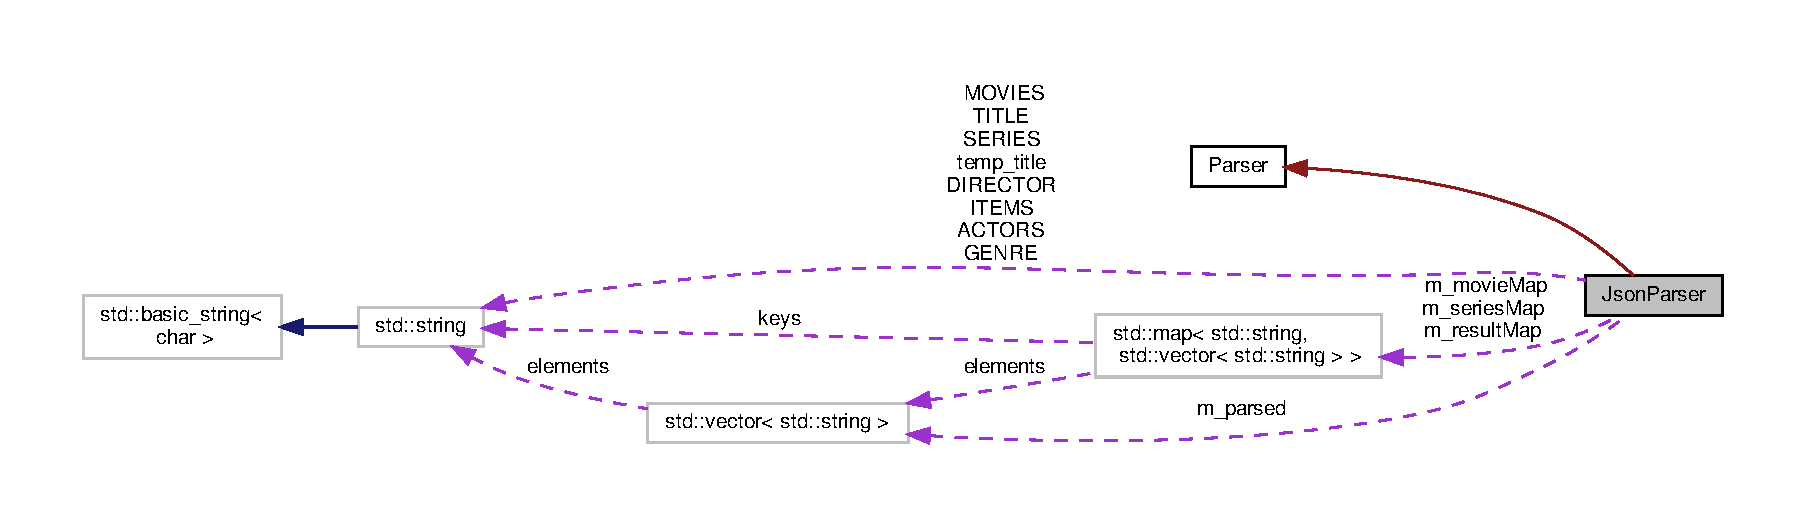
\includegraphics[width=350pt]{classJsonParser__coll__graph}
\end{center}
\end{figure}
\subsection*{Public Member Functions}
\begin{DoxyCompactItemize}
\item 
\mbox{\Hypertarget{classJsonParser_af6b90af892f999ee37dfc57bc0a7851f}\label{classJsonParser_af6b90af892f999ee37dfc57bc0a7851f}} 
{\bfseries Json\+Parser} (\hyperlink{classJsonParser}{Json\+Parser} const \&)=delete
\item 
\mbox{\Hypertarget{classJsonParser_ab4f43720d31047a61275598769b30e7d}\label{classJsonParser_ab4f43720d31047a61275598769b30e7d}} 
void {\bfseries operator=} (\hyperlink{classJsonParser}{Json\+Parser} const \&)=delete
\item 
\mbox{\Hypertarget{classJsonParser_a1d091b22b4f95ea1c16e9d09b644715e}\label{classJsonParser_a1d091b22b4f95ea1c16e9d09b644715e}} 
void {\bfseries clear} () override
\item 
\mbox{\Hypertarget{classJsonParser_abd179a463a5ce61bad930af35bf414d8}\label{classJsonParser_abd179a463a5ce61bad930af35bf414d8}} 
void {\bfseries load} (const Category \&) override
\item 
\mbox{\Hypertarget{classJsonParser_a9ab6146344e60e607289dafe2609c4e5}\label{classJsonParser_a9ab6146344e60e607289dafe2609c4e5}} 
void {\bfseries add} (const Category \&, \hyperlink{classDatabaseItem}{Database\+Item} \&) override
\item 
\mbox{\Hypertarget{classJsonParser_ad49a8004db93e654df391bac2d98c5cc}\label{classJsonParser_ad49a8004db93e654df391bac2d98c5cc}} 
void {\bfseries remove} (const Category \&, \hyperlink{classDatabaseItem}{Database\+Item} \&) override
\item 
\mbox{\Hypertarget{classJsonParser_af5641c4ab20251540d9c9f7a8d182efb}\label{classJsonParser_af5641c4ab20251540d9c9f7a8d182efb}} 
bool {\bfseries find} (Category \&, const std\+::string \&) override
\item 
\mbox{\Hypertarget{classJsonParser_a06078f0464569dac47c5d66131a4f8a4}\label{classJsonParser_a06078f0464569dac47c5d66131a4f8a4}} 
std\+::map$<$ std\+::string, std\+::vector$<$ std\+::string $>$ $>$ {\bfseries get\+Movie\+Parsed} ()
\item 
\mbox{\Hypertarget{classJsonParser_ac942ea55db61a23fd1c6106b76ad1fa4}\label{classJsonParser_ac942ea55db61a23fd1c6106b76ad1fa4}} 
std\+::map$<$ std\+::string, std\+::vector$<$ std\+::string $>$ $>$ {\bfseries get\+Series\+Parsed} ()
\item 
\mbox{\Hypertarget{classJsonParser_ab23dd51f8c905cc86d2ad0b9bf232aeb}\label{classJsonParser_ab23dd51f8c905cc86d2ad0b9bf232aeb}} 
std\+::map$<$ std\+::string, std\+::vector$<$ std\+::string $>$ $>$ {\bfseries get\+Latest\+Result} ()
\end{DoxyCompactItemize}
\subsection*{Static Public Member Functions}
\begin{DoxyCompactItemize}
\item 
\mbox{\Hypertarget{classJsonParser_a31933a8a827a8377b5edbf01bd4a66ac}\label{classJsonParser_a31933a8a827a8377b5edbf01bd4a66ac}} 
static \hyperlink{classJsonParser}{Json\+Parser} \& {\bfseries get\+Instance} ()
\end{DoxyCompactItemize}
\subsection*{Private Attributes}
\begin{DoxyCompactItemize}
\item 
\mbox{\Hypertarget{classJsonParser_a1fd58d33ddee29187d335f9f0cf0a0db}\label{classJsonParser_a1fd58d33ddee29187d335f9f0cf0a0db}} 
const std\+::string {\bfseries T\+I\+T\+LE} = \char`\"{}title\char`\"{}
\item 
\mbox{\Hypertarget{classJsonParser_a32223885ef9b529e156fb47ea847abff}\label{classJsonParser_a32223885ef9b529e156fb47ea847abff}} 
const std\+::string {\bfseries G\+E\+N\+RE} = \char`\"{}genre\char`\"{}
\item 
\mbox{\Hypertarget{classJsonParser_ad47cedc2b9fc664735a9fdcbc9869033}\label{classJsonParser_ad47cedc2b9fc664735a9fdcbc9869033}} 
const std\+::string {\bfseries A\+C\+T\+O\+RS} = \char`\"{}actors\char`\"{}
\item 
\mbox{\Hypertarget{classJsonParser_a8d6aa8c21e729236fd180f051358e9c9}\label{classJsonParser_a8d6aa8c21e729236fd180f051358e9c9}} 
const std\+::string {\bfseries D\+I\+R\+E\+C\+T\+OR} = \char`\"{}director\char`\"{}
\item 
\mbox{\Hypertarget{classJsonParser_a3fcbbf58d72ac41ef6caf67cb34b7864}\label{classJsonParser_a3fcbbf58d72ac41ef6caf67cb34b7864}} 
const std\+::string {\bfseries I\+T\+E\+MS} = \char`\"{}items\char`\"{}
\item 
\mbox{\Hypertarget{classJsonParser_ab209a873c5fa7850d80e9ddc9bab04c0}\label{classJsonParser_ab209a873c5fa7850d80e9ddc9bab04c0}} 
std\+::string {\bfseries M\+O\+V\+I\+ES} = \char`\"{}Movies\char`\"{}
\item 
\mbox{\Hypertarget{classJsonParser_a00fe1d9101a48ef93ee8eeabcc059aae}\label{classJsonParser_a00fe1d9101a48ef93ee8eeabcc059aae}} 
std\+::string {\bfseries S\+E\+R\+I\+ES} = \char`\"{}Series\char`\"{}
\item 
\mbox{\Hypertarget{classJsonParser_ae5a993adef29a11237804dfd3de9fd50}\label{classJsonParser_ae5a993adef29a11237804dfd3de9fd50}} 
Json\+::\+Value {\bfseries m\+\_\+root}
\item 
\mbox{\Hypertarget{classJsonParser_a1947ab7e13cc7917154d7d8aea23f777}\label{classJsonParser_a1947ab7e13cc7917154d7d8aea23f777}} 
std\+::string {\bfseries temp\+\_\+title}
\item 
\mbox{\Hypertarget{classJsonParser_a33e76488d7685330236a52de4a186aba}\label{classJsonParser_a33e76488d7685330236a52de4a186aba}} 
std\+::vector$<$ std\+::string $>$ {\bfseries m\+\_\+parsed}
\item 
\mbox{\Hypertarget{classJsonParser_ad89def06854ea0cf7d21e5d94ad35791}\label{classJsonParser_ad89def06854ea0cf7d21e5d94ad35791}} 
std\+::map$<$ std\+::string, std\+::vector$<$ std\+::string $>$ $>$ {\bfseries m\+\_\+result\+Map}
\item 
\mbox{\Hypertarget{classJsonParser_aa06f285831e0dfeb1218ccdd4a9de41b}\label{classJsonParser_aa06f285831e0dfeb1218ccdd4a9de41b}} 
std\+::map$<$ std\+::string, std\+::vector$<$ std\+::string $>$ $>$ {\bfseries m\+\_\+movie\+Map}
\item 
\mbox{\Hypertarget{classJsonParser_abfa68a2950074daa8b3e64818d104d63}\label{classJsonParser_abfa68a2950074daa8b3e64818d104d63}} 
std\+::map$<$ std\+::string, std\+::vector$<$ std\+::string $>$ $>$ {\bfseries m\+\_\+series\+Map}
\end{DoxyCompactItemize}


The documentation for this class was generated from the following files\+:\begin{DoxyCompactItemize}
\item 
inc/Json\+Parser.\+h\item 
src/Json\+Parser.\+cpp\end{DoxyCompactItemize}

\hypertarget{classJson_1_1LogicError}{}\section{Json\+:\+:Logic\+Error Class Reference}
\label{classJson_1_1LogicError}\index{Json\+::\+Logic\+Error@{Json\+::\+Logic\+Error}}


{\ttfamily \#include $<$json.\+h$>$}



Inheritance diagram for Json\+:\+:Logic\+Error\+:
\nopagebreak
\begin{figure}[H]
\begin{center}
\leavevmode
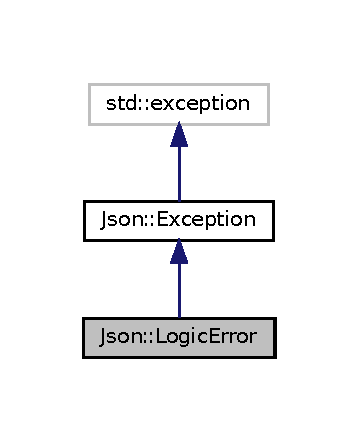
\includegraphics[width=172pt]{classJson_1_1LogicError__inherit__graph}
\end{center}
\end{figure}


Collaboration diagram for Json\+:\+:Logic\+Error\+:
\nopagebreak
\begin{figure}[H]
\begin{center}
\leavevmode
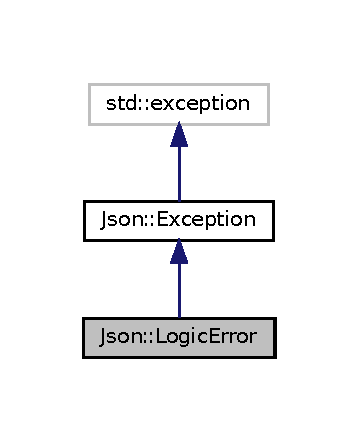
\includegraphics[width=172pt]{classJson_1_1LogicError__coll__graph}
\end{center}
\end{figure}
\subsection*{Public Member Functions}
\begin{DoxyCompactItemize}
\item 
\mbox{\Hypertarget{classJson_1_1LogicError_acca679aa49768a4a1de7b705c67c2919}\label{classJson_1_1LogicError_acca679aa49768a4a1de7b705c67c2919}} 
{\bfseries Logic\+Error} (J\+S\+O\+N\+C\+P\+P\+\_\+\+S\+T\+R\+I\+NG const \&msg)
\end{DoxyCompactItemize}
\subsection*{Additional Inherited Members}


\subsection{Detailed Description}
Exceptions thrown by J\+S\+O\+N\+\_\+\+A\+S\+S\+E\+R\+T/\+J\+S\+O\+N\+\_\+\+F\+A\+IL macros.

These are precondition-\/violations (user bugs) and internal errors (our bugs).

\begin{DoxyRemark}{Remarks}
derived from \hyperlink{classJson_1_1Exception}{Json\+::\+Exception} 
\end{DoxyRemark}


The documentation for this class was generated from the following files\+:\begin{DoxyCompactItemize}
\item 
/home/mjonsson/repo/cpp\+Adv/media\+F\+W/inc/json/json.\+h\item 
/home/mjonsson/repo/cpp\+Adv/media\+F\+W/src/json/jsoncpp.\+cpp\end{DoxyCompactItemize}

\hypertarget{classMovieDatabase}{}\section{Movie\+Database Class Reference}
\label{classMovieDatabase}\index{Movie\+Database@{Movie\+Database}}


A module that implements the functionality of \hyperlink{Database_8h_source}{Database.\+h} and helps the client to perform database actions.  




{\ttfamily \#include $<$Movie\+Database.\+h$>$}



Inheritance diagram for Movie\+Database\+:
\nopagebreak
\begin{figure}[H]
\begin{center}
\leavevmode
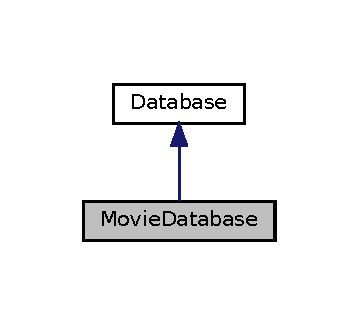
\includegraphics[width=172pt]{classMovieDatabase__inherit__graph}
\end{center}
\end{figure}


Collaboration diagram for Movie\+Database\+:
\nopagebreak
\begin{figure}[H]
\begin{center}
\leavevmode
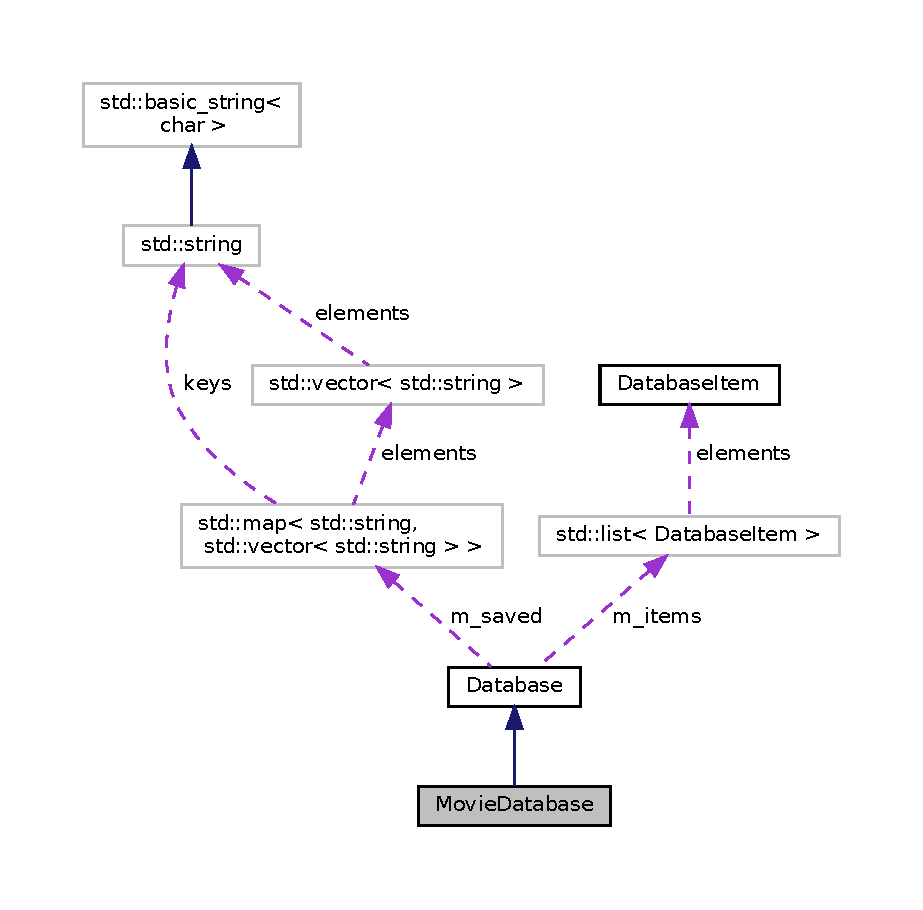
\includegraphics[width=350pt]{classMovieDatabase__coll__graph}
\end{center}
\end{figure}
\subsection*{Public Member Functions}
\begin{DoxyCompactItemize}
\item 
void \hyperlink{classMovieDatabase_a203b9b5c1b325997ce519859a436b6ce}{push\+Item} (const \hyperlink{classDatabaseItem}{Database\+Item} \&m\+\_\+item) override
\begin{DoxyCompactList}\small\item\em Implementation for virtual member of \hyperlink{Database_8h_source}{Database.\+h} Uploads the requested database item. \end{DoxyCompactList}\item 
\hyperlink{classDatabaseItem}{Database\+Item} \hyperlink{classMovieDatabase_ac0bb39b8be599ffea76081809ae42dda}{fetch\+Item} (const std\+::string \&title) override
\begin{DoxyCompactList}\small\item\em Implementation for virtual member of \hyperlink{Database_8h_source}{Database.\+h} Fetch the requested database item. \end{DoxyCompactList}\item 
long \hyperlink{classMovieDatabase_a9a386f51dd72d63414a124cbcfcd879b}{get\+Number\+Of\+Item} () override
\begin{DoxyCompactList}\small\item\em Implementation for virtual member of \hyperlink{Database_8h_source}{Database.\+h} Method that return the size of the database. \end{DoxyCompactList}\item 
void \hyperlink{classMovieDatabase_a85faa4c33b3ab2dc0d1f4939bb034797}{purge\+Item} (const \hyperlink{classDatabaseItem}{Database\+Item} \&m\+\_\+item) override
\begin{DoxyCompactList}\small\item\em Implementation for virtual member of \hyperlink{Database_8h_source}{Database.\+h} Delete the requested database item. \end{DoxyCompactList}\item 
void \hyperlink{classMovieDatabase_af1e13b6fc0fd7186e98edbe2cf187618}{print\+All} () override
\begin{DoxyCompactList}\small\item\em Implementation for virtual member of \hyperlink{Database_8h_source}{Database.\+h} Prints the entire database content. \end{DoxyCompactList}\end{DoxyCompactItemize}
\subsection*{Additional Inherited Members}


\subsection{Detailed Description}
A module that implements the functionality of \hyperlink{Database_8h_source}{Database.\+h} and helps the client to perform database actions. 



\subsection{Member Function Documentation}
\mbox{\Hypertarget{classMovieDatabase_ac0bb39b8be599ffea76081809ae42dda}\label{classMovieDatabase_ac0bb39b8be599ffea76081809ae42dda}} 
\index{Movie\+Database@{Movie\+Database}!fetch\+Item@{fetch\+Item}}
\index{fetch\+Item@{fetch\+Item}!Movie\+Database@{Movie\+Database}}
\subsubsection{\texorpdfstring{fetch\+Item()}{fetchItem()}}
{\footnotesize\ttfamily \hyperlink{classDatabaseItem}{Database\+Item} Movie\+Database\+::fetch\+Item (\begin{DoxyParamCaption}\item[{const std\+::string \&}]{title }\end{DoxyParamCaption})\hspace{0.3cm}{\ttfamily [inline]}, {\ttfamily [override]}, {\ttfamily [virtual]}}



Implementation for virtual member of \hyperlink{Database_8h_source}{Database.\+h} Fetch the requested database item. 

A const reference to a title

\begin{DoxyReturn}{Returns}
The requested \hyperlink{classDatabaseItem}{Database\+Item}
\end{DoxyReturn}


Reimplemented from \hyperlink{classDatabase_a40254eec69c7d7cc15da24a9f0b072b3}{Database}.

\mbox{\Hypertarget{classMovieDatabase_a9a386f51dd72d63414a124cbcfcd879b}\label{classMovieDatabase_a9a386f51dd72d63414a124cbcfcd879b}} 
\index{Movie\+Database@{Movie\+Database}!get\+Number\+Of\+Item@{get\+Number\+Of\+Item}}
\index{get\+Number\+Of\+Item@{get\+Number\+Of\+Item}!Movie\+Database@{Movie\+Database}}
\subsubsection{\texorpdfstring{get\+Number\+Of\+Item()}{getNumberOfItem()}}
{\footnotesize\ttfamily long Movie\+Database\+::get\+Number\+Of\+Item (\begin{DoxyParamCaption}{ }\end{DoxyParamCaption})\hspace{0.3cm}{\ttfamily [inline]}, {\ttfamily [override]}, {\ttfamily [virtual]}}



Implementation for virtual member of \hyperlink{Database_8h_source}{Database.\+h} Method that return the size of the database. 

\begin{DoxyReturn}{Returns}
Size of the database (long).
\end{DoxyReturn}


Reimplemented from \hyperlink{classDatabase_a230225cb341eb23a99a83ef3d1abae53}{Database}.

\mbox{\Hypertarget{classMovieDatabase_af1e13b6fc0fd7186e98edbe2cf187618}\label{classMovieDatabase_af1e13b6fc0fd7186e98edbe2cf187618}} 
\index{Movie\+Database@{Movie\+Database}!print\+All@{print\+All}}
\index{print\+All@{print\+All}!Movie\+Database@{Movie\+Database}}
\subsubsection{\texorpdfstring{print\+All()}{printAll()}}
{\footnotesize\ttfamily void Movie\+Database\+::print\+All (\begin{DoxyParamCaption}{ }\end{DoxyParamCaption})\hspace{0.3cm}{\ttfamily [inline]}, {\ttfamily [override]}, {\ttfamily [virtual]}}



Implementation for virtual member of \hyperlink{Database_8h_source}{Database.\+h} Prints the entire database content. 

\begin{DoxyReturn}{Returns}

\end{DoxyReturn}


Reimplemented from \hyperlink{classDatabase_afa345da530fd5c8dfe0c978917cd6049}{Database}.

\mbox{\Hypertarget{classMovieDatabase_a85faa4c33b3ab2dc0d1f4939bb034797}\label{classMovieDatabase_a85faa4c33b3ab2dc0d1f4939bb034797}} 
\index{Movie\+Database@{Movie\+Database}!purge\+Item@{purge\+Item}}
\index{purge\+Item@{purge\+Item}!Movie\+Database@{Movie\+Database}}
\subsubsection{\texorpdfstring{purge\+Item()}{purgeItem()}}
{\footnotesize\ttfamily void Movie\+Database\+::purge\+Item (\begin{DoxyParamCaption}\item[{const \hyperlink{classDatabaseItem}{Database\+Item} \&}]{m\+\_\+item }\end{DoxyParamCaption})\hspace{0.3cm}{\ttfamily [inline]}, {\ttfamily [override]}, {\ttfamily [virtual]}}



Implementation for virtual member of \hyperlink{Database_8h_source}{Database.\+h} Delete the requested database item. 

A const reference to a database item

\begin{DoxyReturn}{Returns}

\end{DoxyReturn}


Reimplemented from \hyperlink{classDatabase_a5d232b9f62079682dd7fe7983b252e5e}{Database}.

\mbox{\Hypertarget{classMovieDatabase_a203b9b5c1b325997ce519859a436b6ce}\label{classMovieDatabase_a203b9b5c1b325997ce519859a436b6ce}} 
\index{Movie\+Database@{Movie\+Database}!push\+Item@{push\+Item}}
\index{push\+Item@{push\+Item}!Movie\+Database@{Movie\+Database}}
\subsubsection{\texorpdfstring{push\+Item()}{pushItem()}}
{\footnotesize\ttfamily void Movie\+Database\+::push\+Item (\begin{DoxyParamCaption}\item[{const \hyperlink{classDatabaseItem}{Database\+Item} \&}]{m\+\_\+item }\end{DoxyParamCaption})\hspace{0.3cm}{\ttfamily [inline]}, {\ttfamily [override]}, {\ttfamily [virtual]}}



Implementation for virtual member of \hyperlink{Database_8h_source}{Database.\+h} Uploads the requested database item. 

A const reference to a database item

\begin{DoxyReturn}{Returns}

\end{DoxyReturn}


Reimplemented from \hyperlink{classDatabase_a80fa14ab9f4deadc9a2ab7493f1919a4}{Database}.



The documentation for this class was generated from the following file\+:\begin{DoxyCompactItemize}
\item 
/home/mjonsson/repo/cpp\+Adv/media\+F\+W/inc/\+Database/Movie\+Database.\+h\end{DoxyCompactItemize}

\hypertarget{classJson_1_1OurCharReader}{}\section{Json\+:\+:Our\+Char\+Reader Class Reference}
\label{classJson_1_1OurCharReader}\index{Json\+::\+Our\+Char\+Reader@{Json\+::\+Our\+Char\+Reader}}


Inheritance diagram for Json\+:\+:Our\+Char\+Reader\+:
\nopagebreak
\begin{figure}[H]
\begin{center}
\leavevmode
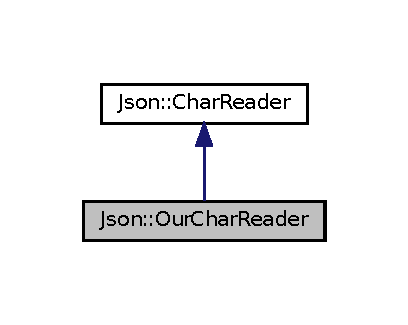
\includegraphics[width=196pt]{classJson_1_1OurCharReader__inherit__graph}
\end{center}
\end{figure}


Collaboration diagram for Json\+:\+:Our\+Char\+Reader\+:
\nopagebreak
\begin{figure}[H]
\begin{center}
\leavevmode
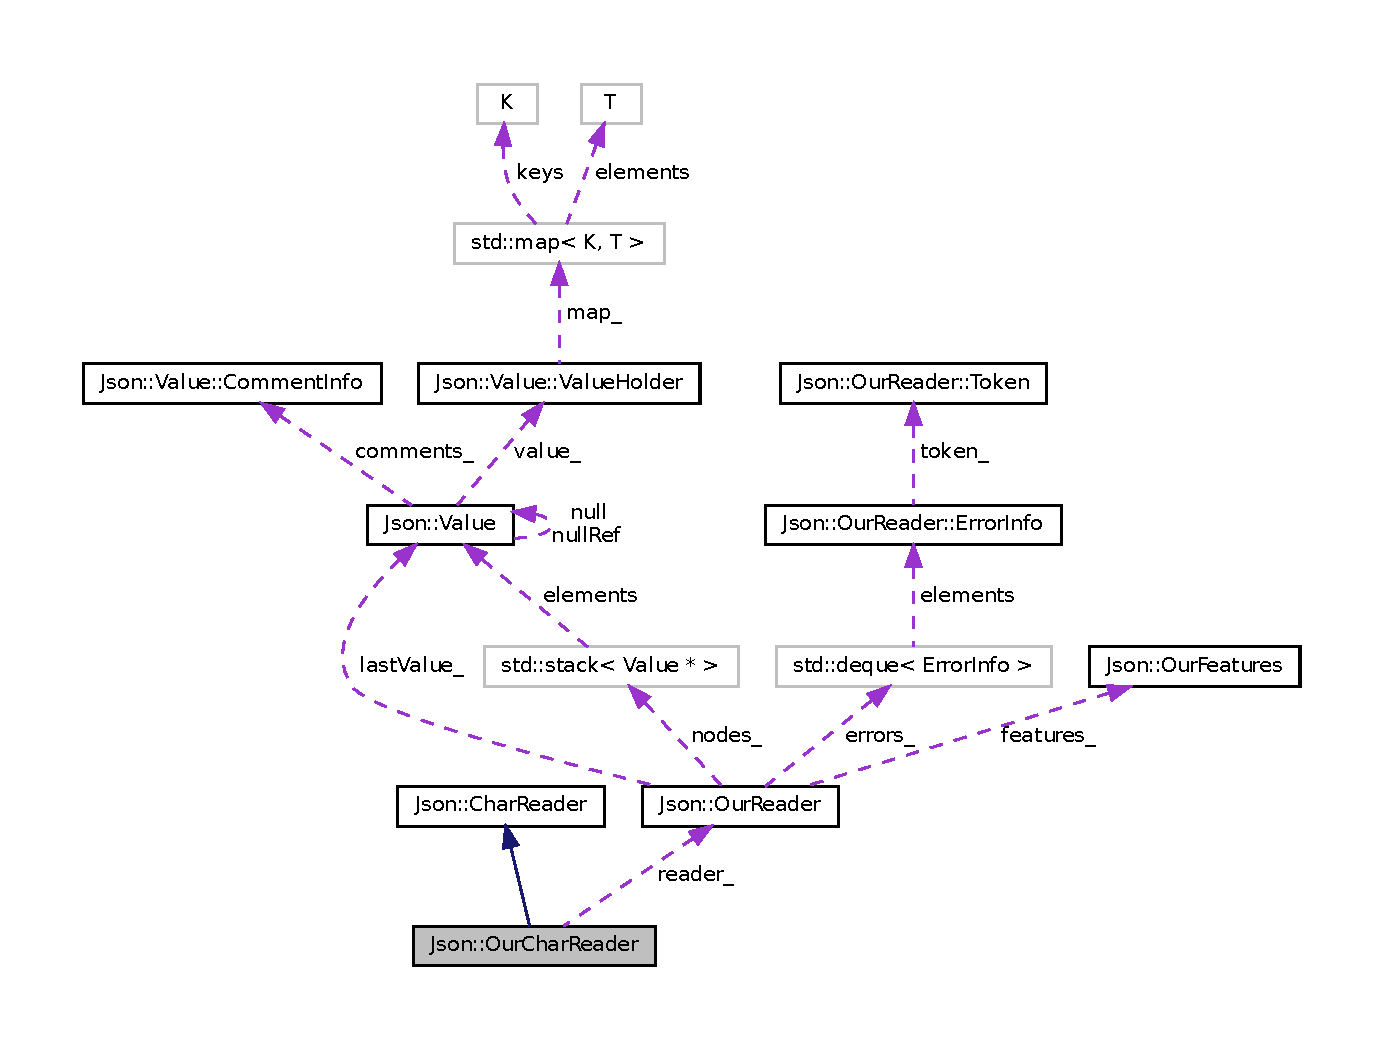
\includegraphics[width=350pt]{classJson_1_1OurCharReader__coll__graph}
\end{center}
\end{figure}
\subsection*{Public Member Functions}
\begin{DoxyCompactItemize}
\item 
\mbox{\Hypertarget{classJson_1_1OurCharReader_a5015506620e7ba7bab417756fa1ca9fe}\label{classJson_1_1OurCharReader_a5015506620e7ba7bab417756fa1ca9fe}} 
{\bfseries Our\+Char\+Reader} (bool collect\+Comments, \hyperlink{classJson_1_1OurFeatures}{Our\+Features} const \&features)
\item 
bool \hyperlink{classJson_1_1OurCharReader_a547f08ec5a9951ca69e8bb2e90296c83}{parse} (char const $\ast$begin\+Doc, char const $\ast$end\+Doc, \hyperlink{classJson_1_1Value}{Value} $\ast$root, J\+S\+O\+N\+C\+P\+P\+\_\+\+S\+T\+R\+I\+NG $\ast$errs) J\+S\+O\+N\+C\+P\+P\+\_\+\+O\+V\+E\+R\+R\+I\+DE
\begin{DoxyCompactList}\small\item\em Read a \hyperlink{classJson_1_1Value}{Value} from a \href{http://www.json.org}{\tt J\+S\+ON} document. The document must be a U\+T\+F-\/8 encoded string containing the document to read. \end{DoxyCompactList}\end{DoxyCompactItemize}
\subsection*{Private Attributes}
\begin{DoxyCompactItemize}
\item 
\mbox{\Hypertarget{classJson_1_1OurCharReader_aa6afd3d0f754cadad0f6d2be38bcfee0}\label{classJson_1_1OurCharReader_aa6afd3d0f754cadad0f6d2be38bcfee0}} 
bool const {\bfseries collect\+Comments\+\_\+}
\item 
\mbox{\Hypertarget{classJson_1_1OurCharReader_aedd4520b8570654ed7aa0726075ee58d}\label{classJson_1_1OurCharReader_aedd4520b8570654ed7aa0726075ee58d}} 
\hyperlink{classJson_1_1OurReader}{Our\+Reader} {\bfseries reader\+\_\+}
\end{DoxyCompactItemize}


\subsection{Member Function Documentation}
\mbox{\Hypertarget{classJson_1_1OurCharReader_a547f08ec5a9951ca69e8bb2e90296c83}\label{classJson_1_1OurCharReader_a547f08ec5a9951ca69e8bb2e90296c83}} 
\index{Json\+::\+Our\+Char\+Reader@{Json\+::\+Our\+Char\+Reader}!parse@{parse}}
\index{parse@{parse}!Json\+::\+Our\+Char\+Reader@{Json\+::\+Our\+Char\+Reader}}
\subsubsection{\texorpdfstring{parse()}{parse()}}
{\footnotesize\ttfamily bool Json\+::\+Our\+Char\+Reader\+::parse (\begin{DoxyParamCaption}\item[{char const $\ast$}]{begin\+Doc,  }\item[{char const $\ast$}]{end\+Doc,  }\item[{\hyperlink{classJson_1_1Value}{Value} $\ast$}]{root,  }\item[{J\+S\+O\+N\+C\+P\+P\+\_\+\+S\+T\+R\+I\+NG $\ast$}]{errs }\end{DoxyParamCaption})\hspace{0.3cm}{\ttfamily [inline]}, {\ttfamily [virtual]}}



Read a \hyperlink{classJson_1_1Value}{Value} from a \href{http://www.json.org}{\tt J\+S\+ON} document. The document must be a U\+T\+F-\/8 encoded string containing the document to read. 


\begin{DoxyParams}{Parameters}
{\em begin\+Doc} & Pointer on the beginning of the U\+T\+F-\/8 encoded string of the document to read. \\
\hline
{\em end\+Doc} & Pointer on the end of the U\+T\+F-\/8 encoded string of the document to read. Must be $>$= begin\+Doc. \\
\hline
{\em root} & \mbox{[}out\mbox{]} Contains the root value of the document if it was successfully parsed. \\
\hline
{\em errs} & \mbox{[}out\mbox{]} Formatted error messages (if not N\+U\+LL) a user friendly string that lists errors in the parsed document. \\
\hline
\end{DoxyParams}
\begin{DoxyReturn}{Returns}
{\ttfamily true} if the document was successfully parsed, {\ttfamily false} if an error occurred. 
\end{DoxyReturn}


Implements \hyperlink{classJson_1_1CharReader_a7983680d50fd0745f371c43b162e78e1}{Json\+::\+Char\+Reader}.



The documentation for this class was generated from the following file\+:\begin{DoxyCompactItemize}
\item 
/home/mjonsson/repo/cpp\+Adv/media\+F\+W/src/json/jsoncpp.\+cpp\end{DoxyCompactItemize}

\hypertarget{classJson_1_1OurFeatures}{}\section{Json\+:\+:Our\+Features Class Reference}
\label{classJson_1_1OurFeatures}\index{Json\+::\+Our\+Features@{Json\+::\+Our\+Features}}
\subsection*{Static Public Member Functions}
\begin{DoxyCompactItemize}
\item 
\mbox{\Hypertarget{classJson_1_1OurFeatures_a0686e1406b6677f496529f9f3fe98d1e}\label{classJson_1_1OurFeatures_a0686e1406b6677f496529f9f3fe98d1e}} 
static \hyperlink{classJson_1_1OurFeatures}{Our\+Features} {\bfseries all} ()
\end{DoxyCompactItemize}
\subsection*{Public Attributes}
\begin{DoxyCompactItemize}
\item 
\mbox{\Hypertarget{classJson_1_1OurFeatures_ac71bb7ba7363d3b05ed76602b036ce33}\label{classJson_1_1OurFeatures_ac71bb7ba7363d3b05ed76602b036ce33}} 
bool {\bfseries allow\+Comments\+\_\+}
\item 
\mbox{\Hypertarget{classJson_1_1OurFeatures_a2095f66a776c0a4ae6cc931a0c94242e}\label{classJson_1_1OurFeatures_a2095f66a776c0a4ae6cc931a0c94242e}} 
bool {\bfseries strict\+Root\+\_\+}
\item 
\mbox{\Hypertarget{classJson_1_1OurFeatures_a13963bc44bf948eec1968f7ff8e8f5f1}\label{classJson_1_1OurFeatures_a13963bc44bf948eec1968f7ff8e8f5f1}} 
bool {\bfseries allow\+Dropped\+Null\+Placeholders\+\_\+}
\item 
\mbox{\Hypertarget{classJson_1_1OurFeatures_af6973fc7e774ce2d634ba99442aeb91a}\label{classJson_1_1OurFeatures_af6973fc7e774ce2d634ba99442aeb91a}} 
bool {\bfseries allow\+Numeric\+Keys\+\_\+}
\item 
\mbox{\Hypertarget{classJson_1_1OurFeatures_abbd6c196d7a22e2a360a59887eda4610}\label{classJson_1_1OurFeatures_abbd6c196d7a22e2a360a59887eda4610}} 
bool {\bfseries allow\+Single\+Quotes\+\_\+}
\item 
\mbox{\Hypertarget{classJson_1_1OurFeatures_ae8ad25b90706c78f1a8fe929191ac61b}\label{classJson_1_1OurFeatures_ae8ad25b90706c78f1a8fe929191ac61b}} 
bool {\bfseries fail\+If\+Extra\+\_\+}
\item 
\mbox{\Hypertarget{classJson_1_1OurFeatures_a39b8e0b86b1c24a45e800c023bb715aa}\label{classJson_1_1OurFeatures_a39b8e0b86b1c24a45e800c023bb715aa}} 
bool {\bfseries reject\+Dup\+Keys\+\_\+}
\item 
\mbox{\Hypertarget{classJson_1_1OurFeatures_af760f91cc2a7af37e44f78fb466061bb}\label{classJson_1_1OurFeatures_af760f91cc2a7af37e44f78fb466061bb}} 
bool {\bfseries allow\+Special\+Floats\+\_\+}
\item 
\mbox{\Hypertarget{classJson_1_1OurFeatures_a9a786713902d14be6d57a08cc03ccfff}\label{classJson_1_1OurFeatures_a9a786713902d14be6d57a08cc03ccfff}} 
int {\bfseries stack\+Limit\+\_\+}
\end{DoxyCompactItemize}


The documentation for this class was generated from the following file\+:\begin{DoxyCompactItemize}
\item 
/home/mjonsson/repo/cpp\+Adv/media\+F\+W/src/jsoncpp.\+cpp\end{DoxyCompactItemize}

\hypertarget{classJson_1_1OurReader}{}\section{Json\+:\+:Our\+Reader Class Reference}
\label{classJson_1_1OurReader}\index{Json\+::\+Our\+Reader@{Json\+::\+Our\+Reader}}


Collaboration diagram for Json\+:\+:Our\+Reader\+:
\nopagebreak
\begin{figure}[H]
\begin{center}
\leavevmode
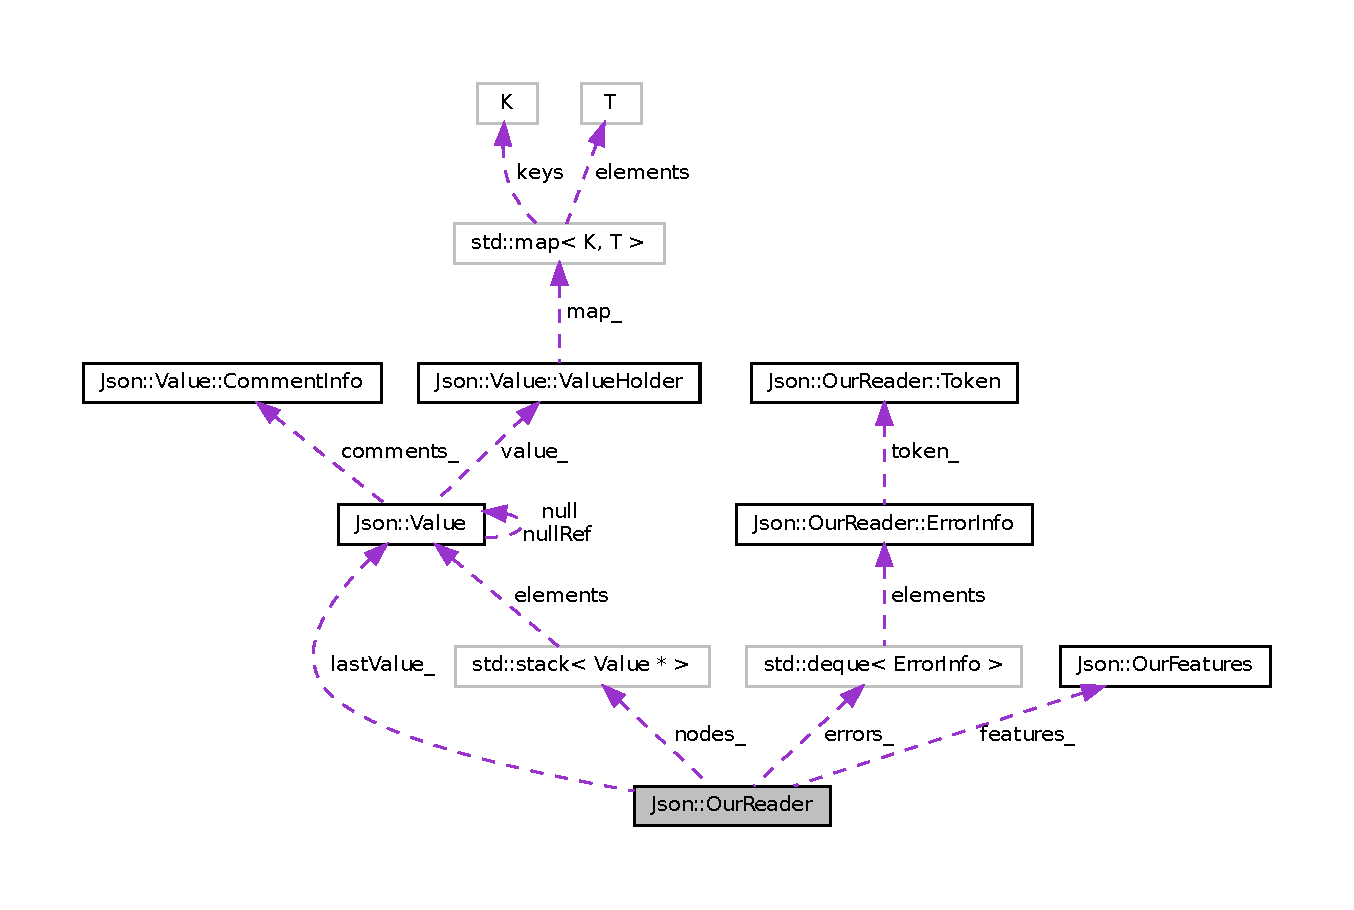
\includegraphics[width=350pt]{classJson_1_1OurReader__coll__graph}
\end{center}
\end{figure}
\subsection*{Classes}
\begin{DoxyCompactItemize}
\item 
class \hyperlink{classJson_1_1OurReader_1_1ErrorInfo}{Error\+Info}
\item 
struct \hyperlink{structJson_1_1OurReader_1_1StructuredError}{Structured\+Error}
\item 
class \hyperlink{classJson_1_1OurReader_1_1Token}{Token}
\end{DoxyCompactItemize}
\subsection*{Public Types}
\begin{DoxyCompactItemize}
\item 
\mbox{\Hypertarget{classJson_1_1OurReader_a0cd0bab4caa66594ab843ccd5f9dc239}\label{classJson_1_1OurReader_a0cd0bab4caa66594ab843ccd5f9dc239}} 
typedef char {\bfseries Char}
\item 
\mbox{\Hypertarget{classJson_1_1OurReader_a1bdc7bbc52ba87cae6b19746f2ee0189}\label{classJson_1_1OurReader_a1bdc7bbc52ba87cae6b19746f2ee0189}} 
typedef const Char $\ast$ {\bfseries Location}
\end{DoxyCompactItemize}
\subsection*{Public Member Functions}
\begin{DoxyCompactItemize}
\item 
\mbox{\Hypertarget{classJson_1_1OurReader_a48a850914b9c8d7781be172930c478e5}\label{classJson_1_1OurReader_a48a850914b9c8d7781be172930c478e5}} 
{\bfseries Our\+Reader} (\hyperlink{classJson_1_1OurFeatures}{Our\+Features} const \&features)
\item 
\mbox{\Hypertarget{classJson_1_1OurReader_aba4f8749aab7f02ec17f107e392caf80}\label{classJson_1_1OurReader_aba4f8749aab7f02ec17f107e392caf80}} 
bool {\bfseries parse} (const char $\ast$begin\+Doc, const char $\ast$end\+Doc, \hyperlink{classJson_1_1Value}{Value} \&root, bool collect\+Comments=true)
\item 
\mbox{\Hypertarget{classJson_1_1OurReader_a7971de51d73bb4aee5b0c4742c4aaaac}\label{classJson_1_1OurReader_a7971de51d73bb4aee5b0c4742c4aaaac}} 
J\+S\+O\+N\+C\+P\+P\+\_\+\+S\+T\+R\+I\+NG {\bfseries get\+Formatted\+Error\+Messages} () const
\item 
\mbox{\Hypertarget{classJson_1_1OurReader_a0eb2420a6bef89a3f3256191e6e3de6d}\label{classJson_1_1OurReader_a0eb2420a6bef89a3f3256191e6e3de6d}} 
std\+::vector$<$ \hyperlink{structJson_1_1OurReader_1_1StructuredError}{Structured\+Error} $>$ {\bfseries get\+Structured\+Errors} () const
\item 
\mbox{\Hypertarget{classJson_1_1OurReader_a700e9d8e0977fa7e0375d26690d7025f}\label{classJson_1_1OurReader_a700e9d8e0977fa7e0375d26690d7025f}} 
bool {\bfseries push\+Error} (const \hyperlink{classJson_1_1Value}{Value} \&value, const J\+S\+O\+N\+C\+P\+P\+\_\+\+S\+T\+R\+I\+NG \&message)
\item 
\mbox{\Hypertarget{classJson_1_1OurReader_addccecfca74b79adaad6115ddd614477}\label{classJson_1_1OurReader_addccecfca74b79adaad6115ddd614477}} 
bool {\bfseries push\+Error} (const \hyperlink{classJson_1_1Value}{Value} \&value, const J\+S\+O\+N\+C\+P\+P\+\_\+\+S\+T\+R\+I\+NG \&message, const \hyperlink{classJson_1_1Value}{Value} \&extra)
\item 
\mbox{\Hypertarget{classJson_1_1OurReader_a63c7d874fa379397e0a5fa65f0843845}\label{classJson_1_1OurReader_a63c7d874fa379397e0a5fa65f0843845}} 
bool {\bfseries good} () const
\end{DoxyCompactItemize}
\subsection*{Private Types}
\begin{DoxyCompactItemize}
\item 
\mbox{\Hypertarget{classJson_1_1OurReader_a15116f7276ddf1e7a2cc3cbefa884dcc}\label{classJson_1_1OurReader_a15116f7276ddf1e7a2cc3cbefa884dcc}} 
enum {\bfseries Token\+Type} \{ \newline
{\bfseries token\+End\+Of\+Stream} = 0, 
{\bfseries token\+Object\+Begin}, 
{\bfseries token\+Object\+End}, 
{\bfseries token\+Array\+Begin}, 
\newline
{\bfseries token\+Array\+End}, 
{\bfseries token\+String}, 
{\bfseries token\+Number}, 
{\bfseries token\+True}, 
\newline
{\bfseries token\+False}, 
{\bfseries token\+Null}, 
{\bfseries token\+NaN}, 
{\bfseries token\+Pos\+Inf}, 
\newline
{\bfseries token\+Neg\+Inf}, 
{\bfseries token\+Array\+Separator}, 
{\bfseries token\+Member\+Separator}, 
{\bfseries token\+Comment}, 
\newline
{\bfseries token\+Error}
 \}
\item 
\mbox{\Hypertarget{classJson_1_1OurReader_a8cc69593ef7303e58e99bb5dbb767562}\label{classJson_1_1OurReader_a8cc69593ef7303e58e99bb5dbb767562}} 
typedef std\+::deque$<$ \hyperlink{classJson_1_1OurReader_1_1ErrorInfo}{Error\+Info} $>$ {\bfseries Errors}
\item 
\mbox{\Hypertarget{classJson_1_1OurReader_a8480a5ef159cee3a090f96358414d8d3}\label{classJson_1_1OurReader_a8480a5ef159cee3a090f96358414d8d3}} 
typedef std\+::stack$<$ \hyperlink{classJson_1_1Value}{Value} $\ast$ $>$ {\bfseries Nodes}
\end{DoxyCompactItemize}
\subsection*{Private Member Functions}
\begin{DoxyCompactItemize}
\item 
\mbox{\Hypertarget{classJson_1_1OurReader_aee013005522c0d34d2e14962851487ac}\label{classJson_1_1OurReader_aee013005522c0d34d2e14962851487ac}} 
{\bfseries Our\+Reader} (\hyperlink{classJson_1_1OurReader}{Our\+Reader} const \&)
\item 
\mbox{\Hypertarget{classJson_1_1OurReader_ad418de7c47bd3d0510888e22110b796e}\label{classJson_1_1OurReader_ad418de7c47bd3d0510888e22110b796e}} 
void {\bfseries operator=} (\hyperlink{classJson_1_1OurReader}{Our\+Reader} const \&)
\item 
\mbox{\Hypertarget{classJson_1_1OurReader_a0d1e66da47fe2e85f5033c59326dfdc3}\label{classJson_1_1OurReader_a0d1e66da47fe2e85f5033c59326dfdc3}} 
bool {\bfseries read\+Token} (\hyperlink{classJson_1_1OurReader_1_1Token}{Token} \&token)
\item 
\mbox{\Hypertarget{classJson_1_1OurReader_a6fbc6d58a4505e5ccadf330b57b17ca5}\label{classJson_1_1OurReader_a6fbc6d58a4505e5ccadf330b57b17ca5}} 
void {\bfseries skip\+Spaces} ()
\item 
\mbox{\Hypertarget{classJson_1_1OurReader_a4a03f1b266def9b47c4fef35386557fb}\label{classJson_1_1OurReader_a4a03f1b266def9b47c4fef35386557fb}} 
bool {\bfseries match} (Location pattern, int pattern\+Length)
\item 
\mbox{\Hypertarget{classJson_1_1OurReader_a90f6bb9e55b2bc3d6c1880809495c222}\label{classJson_1_1OurReader_a90f6bb9e55b2bc3d6c1880809495c222}} 
bool {\bfseries read\+Comment} ()
\item 
\mbox{\Hypertarget{classJson_1_1OurReader_aba784b125baa1b62387e767b791f2f89}\label{classJson_1_1OurReader_aba784b125baa1b62387e767b791f2f89}} 
bool {\bfseries read\+C\+Style\+Comment} ()
\item 
\mbox{\Hypertarget{classJson_1_1OurReader_ae3de80671f0f997053e1c1c8a47a45c5}\label{classJson_1_1OurReader_ae3de80671f0f997053e1c1c8a47a45c5}} 
bool {\bfseries read\+Cpp\+Style\+Comment} ()
\item 
\mbox{\Hypertarget{classJson_1_1OurReader_a5d39b12671499ec5975f3bbc84b7d438}\label{classJson_1_1OurReader_a5d39b12671499ec5975f3bbc84b7d438}} 
bool {\bfseries read\+String} ()
\item 
\mbox{\Hypertarget{classJson_1_1OurReader_ac78592defdc333faf56c6d0908758da3}\label{classJson_1_1OurReader_ac78592defdc333faf56c6d0908758da3}} 
bool {\bfseries read\+String\+Single\+Quote} ()
\item 
\mbox{\Hypertarget{classJson_1_1OurReader_aefcb9a78cc45870ccac2db2a66c8ec50}\label{classJson_1_1OurReader_aefcb9a78cc45870ccac2db2a66c8ec50}} 
bool {\bfseries read\+Number} (bool check\+Inf)
\item 
\mbox{\Hypertarget{classJson_1_1OurReader_a1765d9670d191c89a57a22ea5591d35f}\label{classJson_1_1OurReader_a1765d9670d191c89a57a22ea5591d35f}} 
bool {\bfseries read\+Value} ()
\item 
\mbox{\Hypertarget{classJson_1_1OurReader_aea198f8101dba55099f4d8121a993530}\label{classJson_1_1OurReader_aea198f8101dba55099f4d8121a993530}} 
bool {\bfseries read\+Object} (\hyperlink{classJson_1_1OurReader_1_1Token}{Token} \&token)
\item 
\mbox{\Hypertarget{classJson_1_1OurReader_a0b9f58faf4212c6ecb5d8e2a1ac10257}\label{classJson_1_1OurReader_a0b9f58faf4212c6ecb5d8e2a1ac10257}} 
bool {\bfseries read\+Array} (\hyperlink{classJson_1_1OurReader_1_1Token}{Token} \&token)
\item 
\mbox{\Hypertarget{classJson_1_1OurReader_a272d271290933a89abfd5096dd69c9e9}\label{classJson_1_1OurReader_a272d271290933a89abfd5096dd69c9e9}} 
bool {\bfseries decode\+Number} (\hyperlink{classJson_1_1OurReader_1_1Token}{Token} \&token)
\item 
\mbox{\Hypertarget{classJson_1_1OurReader_a712270d53a2f023c2f406ac813548340}\label{classJson_1_1OurReader_a712270d53a2f023c2f406ac813548340}} 
bool {\bfseries decode\+Number} (\hyperlink{classJson_1_1OurReader_1_1Token}{Token} \&token, \hyperlink{classJson_1_1Value}{Value} \&decoded)
\item 
\mbox{\Hypertarget{classJson_1_1OurReader_a34e31d8b8399b7ad493359702b6de6c9}\label{classJson_1_1OurReader_a34e31d8b8399b7ad493359702b6de6c9}} 
bool {\bfseries decode\+String} (\hyperlink{classJson_1_1OurReader_1_1Token}{Token} \&token)
\item 
\mbox{\Hypertarget{classJson_1_1OurReader_a5046dfa5d43b1770a091aac0a63a9f4b}\label{classJson_1_1OurReader_a5046dfa5d43b1770a091aac0a63a9f4b}} 
bool {\bfseries decode\+String} (\hyperlink{classJson_1_1OurReader_1_1Token}{Token} \&token, J\+S\+O\+N\+C\+P\+P\+\_\+\+S\+T\+R\+I\+NG \&decoded)
\item 
\mbox{\Hypertarget{classJson_1_1OurReader_a1d1c3b44f6720a0e7c39b5ae8de3981c}\label{classJson_1_1OurReader_a1d1c3b44f6720a0e7c39b5ae8de3981c}} 
bool {\bfseries decode\+Double} (\hyperlink{classJson_1_1OurReader_1_1Token}{Token} \&token)
\item 
\mbox{\Hypertarget{classJson_1_1OurReader_aa5c15a8cd32754f07430dedba3d1308e}\label{classJson_1_1OurReader_aa5c15a8cd32754f07430dedba3d1308e}} 
bool {\bfseries decode\+Double} (\hyperlink{classJson_1_1OurReader_1_1Token}{Token} \&token, \hyperlink{classJson_1_1Value}{Value} \&decoded)
\item 
\mbox{\Hypertarget{classJson_1_1OurReader_ac1bf03c161ece082e48da450c50f528d}\label{classJson_1_1OurReader_ac1bf03c161ece082e48da450c50f528d}} 
bool {\bfseries decode\+Unicode\+Code\+Point} (\hyperlink{classJson_1_1OurReader_1_1Token}{Token} \&token, Location \&current, Location end, unsigned int \&unicode)
\item 
\mbox{\Hypertarget{classJson_1_1OurReader_adb39be814cc6076b91a0919bdd5b24b0}\label{classJson_1_1OurReader_adb39be814cc6076b91a0919bdd5b24b0}} 
bool {\bfseries decode\+Unicode\+Escape\+Sequence} (\hyperlink{classJson_1_1OurReader_1_1Token}{Token} \&token, Location \&current, Location end, unsigned int \&unicode)
\item 
\mbox{\Hypertarget{classJson_1_1OurReader_aa6a920311e6408ff3a45324d49da18a6}\label{classJson_1_1OurReader_aa6a920311e6408ff3a45324d49da18a6}} 
bool {\bfseries add\+Error} (const J\+S\+O\+N\+C\+P\+P\+\_\+\+S\+T\+R\+I\+NG \&message, \hyperlink{classJson_1_1OurReader_1_1Token}{Token} \&token, Location extra=0)
\item 
\mbox{\Hypertarget{classJson_1_1OurReader_a035651f0700a76a815e5f904c63ebb1c}\label{classJson_1_1OurReader_a035651f0700a76a815e5f904c63ebb1c}} 
bool {\bfseries recover\+From\+Error} (Token\+Type skip\+Until\+Token)
\item 
\mbox{\Hypertarget{classJson_1_1OurReader_a074cf3d91e9404fe89e03cfc6a43e6fb}\label{classJson_1_1OurReader_a074cf3d91e9404fe89e03cfc6a43e6fb}} 
bool {\bfseries add\+Error\+And\+Recover} (const J\+S\+O\+N\+C\+P\+P\+\_\+\+S\+T\+R\+I\+NG \&message, \hyperlink{classJson_1_1OurReader_1_1Token}{Token} \&token, Token\+Type skip\+Until\+Token)
\item 
\mbox{\Hypertarget{classJson_1_1OurReader_ad48bdaf5b686706f003e792fdbcbf102}\label{classJson_1_1OurReader_ad48bdaf5b686706f003e792fdbcbf102}} 
void {\bfseries skip\+Until\+Space} ()
\item 
\mbox{\Hypertarget{classJson_1_1OurReader_a2acd5b1d53e7d7e17c21ff8e96edc09d}\label{classJson_1_1OurReader_a2acd5b1d53e7d7e17c21ff8e96edc09d}} 
\hyperlink{classJson_1_1Value}{Value} \& {\bfseries current\+Value} ()
\item 
\mbox{\Hypertarget{classJson_1_1OurReader_a298285d035fdbc554caae09d9f0a5859}\label{classJson_1_1OurReader_a298285d035fdbc554caae09d9f0a5859}} 
Char {\bfseries get\+Next\+Char} ()
\item 
\mbox{\Hypertarget{classJson_1_1OurReader_af482c8e718615646e13a996292e18d74}\label{classJson_1_1OurReader_af482c8e718615646e13a996292e18d74}} 
void {\bfseries get\+Location\+Line\+And\+Column} (Location location, int \&line, int \&column) const
\item 
\mbox{\Hypertarget{classJson_1_1OurReader_ac129e94cdc260822b2fd24e2ca35e636}\label{classJson_1_1OurReader_ac129e94cdc260822b2fd24e2ca35e636}} 
J\+S\+O\+N\+C\+P\+P\+\_\+\+S\+T\+R\+I\+NG {\bfseries get\+Location\+Line\+And\+Column} (Location location) const
\item 
\mbox{\Hypertarget{classJson_1_1OurReader_ad7318c37469a9106069a236fb4b10e1f}\label{classJson_1_1OurReader_ad7318c37469a9106069a236fb4b10e1f}} 
void {\bfseries add\+Comment} (Location begin, Location end, \hyperlink{namespaceJson_a4fc417c23905b2ae9e2c47d197a45351}{Comment\+Placement} placement)
\item 
\mbox{\Hypertarget{classJson_1_1OurReader_a856dea44d92578c276856d7a65a4ebdc}\label{classJson_1_1OurReader_a856dea44d92578c276856d7a65a4ebdc}} 
void {\bfseries skip\+Comment\+Tokens} (\hyperlink{classJson_1_1OurReader_1_1Token}{Token} \&token)
\end{DoxyCompactItemize}
\subsection*{Static Private Member Functions}
\begin{DoxyCompactItemize}
\item 
\mbox{\Hypertarget{classJson_1_1OurReader_a73ec369ee36598e008b80e36263691be}\label{classJson_1_1OurReader_a73ec369ee36598e008b80e36263691be}} 
static J\+S\+O\+N\+C\+P\+P\+\_\+\+S\+T\+R\+I\+NG {\bfseries normalize\+E\+OL} (Location begin, Location end)
\item 
\mbox{\Hypertarget{classJson_1_1OurReader_ab9e83f5a3d9dab2dabce367a4faa2b1b}\label{classJson_1_1OurReader_ab9e83f5a3d9dab2dabce367a4faa2b1b}} 
static bool {\bfseries contains\+New\+Line} (Location begin, Location end)
\end{DoxyCompactItemize}
\subsection*{Private Attributes}
\begin{DoxyCompactItemize}
\item 
\mbox{\Hypertarget{classJson_1_1OurReader_a19cc4e8c5d17ee6822f752e9a36f4ce3}\label{classJson_1_1OurReader_a19cc4e8c5d17ee6822f752e9a36f4ce3}} 
Nodes {\bfseries nodes\+\_\+}
\item 
\mbox{\Hypertarget{classJson_1_1OurReader_afb76b68ba1ab68fe09cf2838e3d4898d}\label{classJson_1_1OurReader_afb76b68ba1ab68fe09cf2838e3d4898d}} 
Errors {\bfseries errors\+\_\+}
\item 
\mbox{\Hypertarget{classJson_1_1OurReader_a726230af83d22d25e0c76cec3408ecf1}\label{classJson_1_1OurReader_a726230af83d22d25e0c76cec3408ecf1}} 
J\+S\+O\+N\+C\+P\+P\+\_\+\+S\+T\+R\+I\+NG {\bfseries document\+\_\+}
\item 
\mbox{\Hypertarget{classJson_1_1OurReader_a9bda9d72335d52cd06e65f9eca3f70f5}\label{classJson_1_1OurReader_a9bda9d72335d52cd06e65f9eca3f70f5}} 
Location {\bfseries begin\+\_\+}
\item 
\mbox{\Hypertarget{classJson_1_1OurReader_ab1f69b0260c27a0d2d65dc56e42c8f9d}\label{classJson_1_1OurReader_ab1f69b0260c27a0d2d65dc56e42c8f9d}} 
Location {\bfseries end\+\_\+}
\item 
\mbox{\Hypertarget{classJson_1_1OurReader_a5211fbbba94be80a22dd2317c621efcc}\label{classJson_1_1OurReader_a5211fbbba94be80a22dd2317c621efcc}} 
Location {\bfseries current\+\_\+}
\item 
\mbox{\Hypertarget{classJson_1_1OurReader_a101eadc45e01c60628b53f0db3d13482}\label{classJson_1_1OurReader_a101eadc45e01c60628b53f0db3d13482}} 
Location {\bfseries last\+Value\+End\+\_\+}
\item 
\mbox{\Hypertarget{classJson_1_1OurReader_a9f994b6a2227c5d96e6ed6cbc74ed251}\label{classJson_1_1OurReader_a9f994b6a2227c5d96e6ed6cbc74ed251}} 
\hyperlink{classJson_1_1Value}{Value} $\ast$ {\bfseries last\+Value\+\_\+}
\item 
\mbox{\Hypertarget{classJson_1_1OurReader_a9c53e77e290eb9081298210a955fda6a}\label{classJson_1_1OurReader_a9c53e77e290eb9081298210a955fda6a}} 
J\+S\+O\+N\+C\+P\+P\+\_\+\+S\+T\+R\+I\+NG {\bfseries comments\+Before\+\_\+}
\item 
\mbox{\Hypertarget{classJson_1_1OurReader_a2714302d5cc54ca2ce4118ea51c0397a}\label{classJson_1_1OurReader_a2714302d5cc54ca2ce4118ea51c0397a}} 
\hyperlink{classJson_1_1OurFeatures}{Our\+Features} const {\bfseries features\+\_\+}
\item 
\mbox{\Hypertarget{classJson_1_1OurReader_a259f6ac988da2894bcafc670e42f73ad}\label{classJson_1_1OurReader_a259f6ac988da2894bcafc670e42f73ad}} 
bool {\bfseries collect\+Comments\+\_\+}
\end{DoxyCompactItemize}


The documentation for this class was generated from the following file\+:\begin{DoxyCompactItemize}
\item 
/home/mjonsson/repo/cpp\+Adv/media\+F\+W/src/json/jsoncpp.\+cpp\end{DoxyCompactItemize}

\hypertarget{classJson_1_1Path}{}\section{Json\+:\+:Path Class Reference}
\label{classJson_1_1Path}\index{Json\+::\+Path@{Json\+::\+Path}}


Experimental and untested\+: represents a \char`\"{}path\char`\"{} to access a node.  




{\ttfamily \#include $<$json.\+h$>$}

\subsection*{Public Member Functions}
\begin{DoxyCompactItemize}
\item 
\mbox{\Hypertarget{classJson_1_1Path_a7356c0e9c1fc2276390fd396271c1300}\label{classJson_1_1Path_a7356c0e9c1fc2276390fd396271c1300}} 
{\bfseries Path} (const J\+S\+O\+N\+C\+P\+P\+\_\+\+S\+T\+R\+I\+NG \&path, const \hyperlink{classJson_1_1PathArgument}{Path\+Argument} \&a1=\hyperlink{classJson_1_1PathArgument}{Path\+Argument}(), const \hyperlink{classJson_1_1PathArgument}{Path\+Argument} \&a2=\hyperlink{classJson_1_1PathArgument}{Path\+Argument}(), const \hyperlink{classJson_1_1PathArgument}{Path\+Argument} \&a3=\hyperlink{classJson_1_1PathArgument}{Path\+Argument}(), const \hyperlink{classJson_1_1PathArgument}{Path\+Argument} \&a4=\hyperlink{classJson_1_1PathArgument}{Path\+Argument}(), const \hyperlink{classJson_1_1PathArgument}{Path\+Argument} \&a5=\hyperlink{classJson_1_1PathArgument}{Path\+Argument}())
\item 
\mbox{\Hypertarget{classJson_1_1Path_ad1abdc54d2e03fc0e9436c3b9fd55a33}\label{classJson_1_1Path_ad1abdc54d2e03fc0e9436c3b9fd55a33}} 
const \hyperlink{classJson_1_1Value}{Value} \& {\bfseries resolve} (const \hyperlink{classJson_1_1Value}{Value} \&root) const
\item 
\mbox{\Hypertarget{classJson_1_1Path_ab65ab001ccdbc6f8b5f123da58b92539}\label{classJson_1_1Path_ab65ab001ccdbc6f8b5f123da58b92539}} 
\hyperlink{classJson_1_1Value}{Value} {\bfseries resolve} (const \hyperlink{classJson_1_1Value}{Value} \&root, const \hyperlink{classJson_1_1Value}{Value} \&default\+Value) const
\item 
\hyperlink{classJson_1_1Value}{Value} \& \hyperlink{classJson_1_1Path_a858f9426f0f7bbe0450644d72b44e26b}{make} (\hyperlink{classJson_1_1Value}{Value} \&root) const
\end{DoxyCompactItemize}


\subsection{Detailed Description}
Experimental and untested\+: represents a \char`\"{}path\char`\"{} to access a node. 

Syntax\+:
\begin{DoxyItemize}
\item \char`\"{}.\char`\"{} =$>$ root node
\item \char`\"{}.\mbox{[}n\mbox{]}\char`\"{} =$>$ elements at index \textquotesingle{}n\textquotesingle{} of root node (an array value)
\item \char`\"{}.\+name\char`\"{} =$>$ member named \textquotesingle{}name\textquotesingle{} of root node (an object value)
\item \char`\"{}.\+name1.\+name2.\+name3\char`\"{}
\item \char`\"{}.\mbox{[}0\mbox{]}\mbox{[}1\mbox{]}\mbox{[}2\mbox{]}.\+name1\mbox{[}3\mbox{]}\char`\"{}
\item \char`\"{}.\%\char`\"{} =$>$ member name is provided as parameter
\item \char`\"{}.\mbox{[}\%\mbox{]}\char`\"{} =$>$ index is provied as parameter 
\end{DoxyItemize}

\subsection{Member Function Documentation}
\mbox{\Hypertarget{classJson_1_1Path_a858f9426f0f7bbe0450644d72b44e26b}\label{classJson_1_1Path_a858f9426f0f7bbe0450644d72b44e26b}} 
\index{Json\+::\+Path@{Json\+::\+Path}!make@{make}}
\index{make@{make}!Json\+::\+Path@{Json\+::\+Path}}
\subsubsection{\texorpdfstring{make()}{make()}}
{\footnotesize\ttfamily \hyperlink{classJson_1_1Value}{Value} \& Json\+::\+Path\+::make (\begin{DoxyParamCaption}\item[{\hyperlink{classJson_1_1Value}{Value} \&}]{root }\end{DoxyParamCaption}) const}

Creates the \char`\"{}path\char`\"{} to access the specified node and returns a reference on the node. 

The documentation for this class was generated from the following files\+:\begin{DoxyCompactItemize}
\item 
/home/mjonsson/repo/cpp\+Adv/media\+F\+W/inc/json/json.\+h\item 
/home/mjonsson/repo/cpp\+Adv/media\+F\+W/src/jsoncpp.\+cpp\end{DoxyCompactItemize}

\hypertarget{classJson_1_1PathArgument}{}\section{Json\+:\+:Path\+Argument Class Reference}
\label{classJson_1_1PathArgument}\index{Json\+::\+Path\+Argument@{Json\+::\+Path\+Argument}}


Experimental and untested\+: represents an element of the \char`\"{}path\char`\"{} to access a node.  




{\ttfamily \#include $<$json.\+h$>$}

\subsection*{Public Member Functions}
\begin{DoxyCompactItemize}
\item 
\mbox{\Hypertarget{classJson_1_1PathArgument_a53c5b27143b161301b95fd544c139ecf}\label{classJson_1_1PathArgument_a53c5b27143b161301b95fd544c139ecf}} 
{\bfseries Path\+Argument} (Array\+Index index)
\item 
\mbox{\Hypertarget{classJson_1_1PathArgument_a9690417a8a40e6e49f2acdf6c9281345}\label{classJson_1_1PathArgument_a9690417a8a40e6e49f2acdf6c9281345}} 
{\bfseries Path\+Argument} (const char $\ast$key)
\item 
\mbox{\Hypertarget{classJson_1_1PathArgument_ac15f25452124fbf21218897113015301}\label{classJson_1_1PathArgument_ac15f25452124fbf21218897113015301}} 
{\bfseries Path\+Argument} (const J\+S\+O\+N\+C\+P\+P\+\_\+\+S\+T\+R\+I\+NG \&key)
\end{DoxyCompactItemize}
\subsection*{Private Types}
\begin{DoxyCompactItemize}
\item 
\mbox{\Hypertarget{classJson_1_1PathArgument_a2420bbad778573c147e578701b84d9b9}\label{classJson_1_1PathArgument_a2420bbad778573c147e578701b84d9b9}} 
enum {\bfseries Kind} \{ {\bfseries kind\+None} = 0, 
{\bfseries kind\+Index}, 
{\bfseries kind\+Key}
 \}
\end{DoxyCompactItemize}
\subsection*{Private Attributes}
\begin{DoxyCompactItemize}
\item 
\mbox{\Hypertarget{classJson_1_1PathArgument_af4024368548ff730ef2bed97d6f1ca43}\label{classJson_1_1PathArgument_af4024368548ff730ef2bed97d6f1ca43}} 
J\+S\+O\+N\+C\+P\+P\+\_\+\+S\+T\+R\+I\+NG {\bfseries key\+\_\+}
\item 
\mbox{\Hypertarget{classJson_1_1PathArgument_afd5857d1b6bfaae6961333bdae7bd5ec}\label{classJson_1_1PathArgument_afd5857d1b6bfaae6961333bdae7bd5ec}} 
Array\+Index {\bfseries index\+\_\+}
\item 
\mbox{\Hypertarget{classJson_1_1PathArgument_ad4bc4b544b155a3d9c7788572ecf991b}\label{classJson_1_1PathArgument_ad4bc4b544b155a3d9c7788572ecf991b}} 
Kind {\bfseries kind\+\_\+}
\end{DoxyCompactItemize}
\subsection*{Friends}
\begin{DoxyCompactItemize}
\item 
\mbox{\Hypertarget{classJson_1_1PathArgument_a4877239a6b7f09fbf5a61ca68a49d74c}\label{classJson_1_1PathArgument_a4877239a6b7f09fbf5a61ca68a49d74c}} 
class {\bfseries Path}
\end{DoxyCompactItemize}


\subsection{Detailed Description}
Experimental and untested\+: represents an element of the \char`\"{}path\char`\"{} to access a node. 

The documentation for this class was generated from the following files\+:\begin{DoxyCompactItemize}
\item 
/home/mjonsson/repo/cpp\+Adv/media\+F\+W/inc/json/json.\+h\item 
/home/mjonsson/repo/cpp\+Adv/media\+F\+W/src/json/jsoncpp.\+cpp\end{DoxyCompactItemize}

\hypertarget{classJson_1_1Reader}{}\section{Json\+:\+:Reader Class Reference}
\label{classJson_1_1Reader}\index{Json\+::\+Reader@{Json\+::\+Reader}}


Unserialize a \href{http://www.json.org}{\tt J\+S\+ON} document into a \hyperlink{classJson_1_1Value}{Value}.  




{\ttfamily \#include $<$json.\+h$>$}



Collaboration diagram for Json\+:\+:Reader\+:
\nopagebreak
\begin{figure}[H]
\begin{center}
\leavevmode
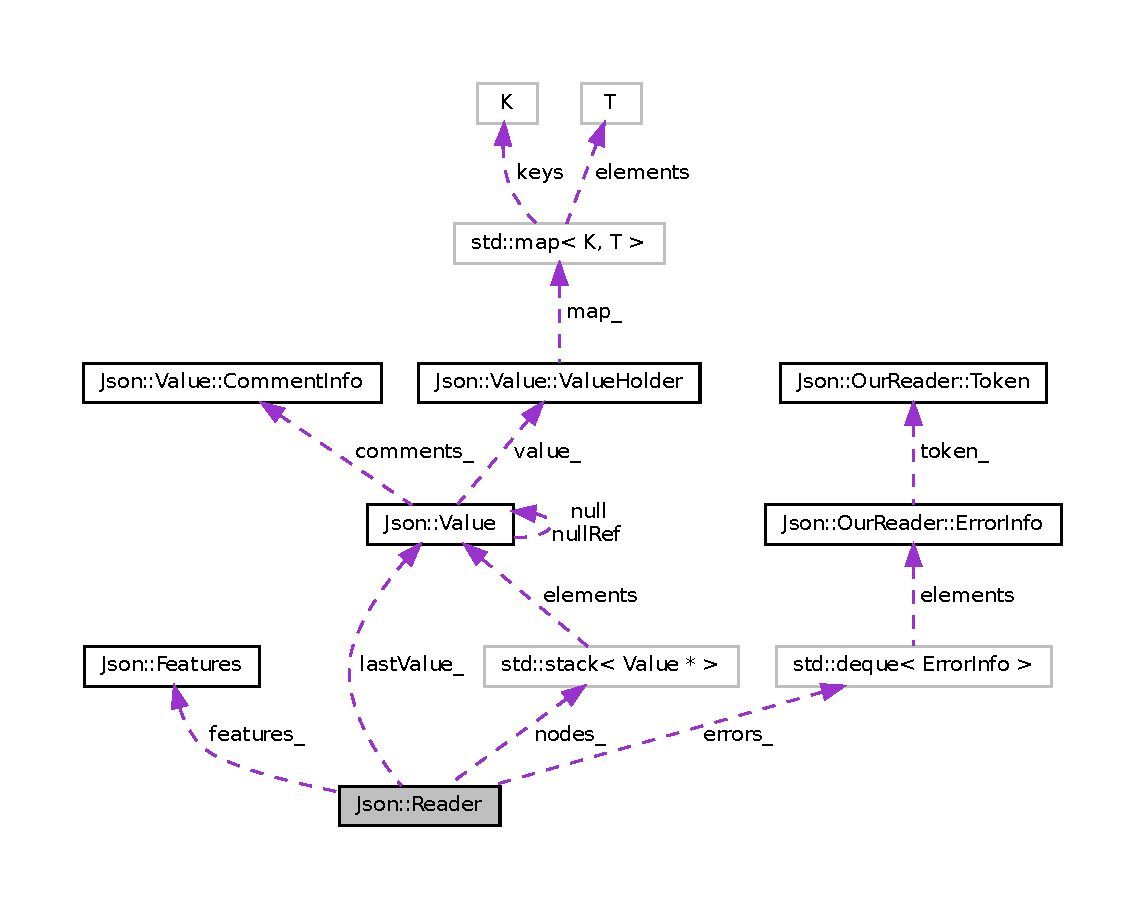
\includegraphics[width=350pt]{classJson_1_1Reader__coll__graph}
\end{center}
\end{figure}
\subsection*{Classes}
\begin{DoxyCompactItemize}
\item 
class \hyperlink{classJson_1_1Reader_1_1ErrorInfo}{Error\+Info}
\item 
struct \hyperlink{structJson_1_1Reader_1_1StructuredError}{Structured\+Error}
\begin{DoxyCompactList}\small\item\em An error tagged with where in the J\+S\+ON text it was encountered. \end{DoxyCompactList}\item 
class \hyperlink{classJson_1_1Reader_1_1Token}{Token}
\end{DoxyCompactItemize}
\subsection*{Public Types}
\begin{DoxyCompactItemize}
\item 
\mbox{\Hypertarget{classJson_1_1Reader_a3eec9118f3e9a672ba8348c3a79d0f45}\label{classJson_1_1Reader_a3eec9118f3e9a672ba8348c3a79d0f45}} 
typedef char {\bfseries Char}
\item 
\mbox{\Hypertarget{classJson_1_1Reader_a46795b5b272bf79a7730e406cb96375a}\label{classJson_1_1Reader_a46795b5b272bf79a7730e406cb96375a}} 
typedef const Char $\ast$ {\bfseries Location}
\end{DoxyCompactItemize}
\subsection*{Public Member Functions}
\begin{DoxyCompactItemize}
\item 
\mbox{\Hypertarget{classJson_1_1Reader_a0b3c4e24c8393354bab57a6ba3ffc27f}\label{classJson_1_1Reader_a0b3c4e24c8393354bab57a6ba3ffc27f}} 
\hyperlink{classJson_1_1Reader_a0b3c4e24c8393354bab57a6ba3ffc27f}{Reader} ()
\begin{DoxyCompactList}\small\item\em Constructs a \hyperlink{classJson_1_1Reader}{Reader} allowing all features for parsing. \end{DoxyCompactList}\item 
\mbox{\Hypertarget{classJson_1_1Reader_a45f17831118337309180313e93ac33f8}\label{classJson_1_1Reader_a45f17831118337309180313e93ac33f8}} 
\hyperlink{classJson_1_1Reader_a45f17831118337309180313e93ac33f8}{Reader} (const \hyperlink{classJson_1_1Features}{Features} \&features)
\begin{DoxyCompactList}\small\item\em Constructs a \hyperlink{classJson_1_1Reader}{Reader} allowing the specified feature set for parsing. \end{DoxyCompactList}\item 
bool \hyperlink{classJson_1_1Reader_af1da6c976ad1e96c742804c3853eef94}{parse} (const std\+::string \&document, \hyperlink{classJson_1_1Value}{Value} \&root, bool collect\+Comments=true)
\begin{DoxyCompactList}\small\item\em Read a \hyperlink{classJson_1_1Value}{Value} from a \href{http://www.json.org}{\tt J\+S\+ON} document. \end{DoxyCompactList}\item 
bool \hyperlink{classJson_1_1Reader_ac71ef2b64c7c27b062052e692af3fb32}{parse} (const char $\ast$begin\+Doc, const char $\ast$end\+Doc, \hyperlink{classJson_1_1Value}{Value} \&root, bool collect\+Comments=true)
\begin{DoxyCompactList}\small\item\em Read a \hyperlink{classJson_1_1Value}{Value} from a \href{http://www.json.org}{\tt J\+S\+ON} document. \end{DoxyCompactList}\item 
bool \hyperlink{classJson_1_1Reader_a6d5d0e23f68749d2f17feece4ccf504d}{parse} (J\+S\+O\+N\+C\+P\+P\+\_\+\+I\+S\+T\+R\+E\+AM \&is, \hyperlink{classJson_1_1Value}{Value} \&root, bool collect\+Comments=true)
\begin{DoxyCompactList}\small\item\em Parse from input stream. \end{DoxyCompactList}\item 
J\+S\+O\+N\+C\+P\+P\+\_\+\+S\+T\+R\+I\+NG \hyperlink{classJson_1_1Reader_a791cbc5afd1bef1631e07239dc452c79}{get\+Formated\+Error\+Messages} () const
\begin{DoxyCompactList}\small\item\em Returns a user friendly string that list errors in the parsed document. \end{DoxyCompactList}\item 
J\+S\+O\+N\+C\+P\+P\+\_\+\+S\+T\+R\+I\+NG \hyperlink{classJson_1_1Reader_ae638a7b1f36f7ccf99ba89fa36ccf222}{get\+Formatted\+Error\+Messages} () const
\begin{DoxyCompactList}\small\item\em Returns a user friendly string that list errors in the parsed document. \end{DoxyCompactList}\item 
std\+::vector$<$ \hyperlink{structJson_1_1Reader_1_1StructuredError}{Structured\+Error} $>$ \hyperlink{classJson_1_1Reader_ae3d714e95bd98b27e296c607e408189b}{get\+Structured\+Errors} () const
\begin{DoxyCompactList}\small\item\em Returns a vector of structured erros encounted while parsing. \end{DoxyCompactList}\item 
bool \hyperlink{classJson_1_1Reader_af5fa7099083f01706635ade1d0f8ddb5}{push\+Error} (const \hyperlink{classJson_1_1Value}{Value} \&value, const J\+S\+O\+N\+C\+P\+P\+\_\+\+S\+T\+R\+I\+NG \&message)
\begin{DoxyCompactList}\small\item\em Add a semantic error message. \end{DoxyCompactList}\item 
bool \hyperlink{classJson_1_1Reader_a3568be9db568ff57bd3fcc373143dff3}{push\+Error} (const \hyperlink{classJson_1_1Value}{Value} \&value, const J\+S\+O\+N\+C\+P\+P\+\_\+\+S\+T\+R\+I\+NG \&message, const \hyperlink{classJson_1_1Value}{Value} \&extra)
\begin{DoxyCompactList}\small\item\em Add a semantic error message with extra context. \end{DoxyCompactList}\item 
bool \hyperlink{classJson_1_1Reader_a86cbb42b3e6d4a4d6416473b1a8f6ae7}{good} () const
\begin{DoxyCompactList}\small\item\em Return whether there are any errors. \end{DoxyCompactList}\end{DoxyCompactItemize}
\subsection*{Private Types}
\begin{DoxyCompactItemize}
\item 
\mbox{\Hypertarget{classJson_1_1Reader_aa35e6ab574dc399a0a645ad98ed66bc9}\label{classJson_1_1Reader_aa35e6ab574dc399a0a645ad98ed66bc9}} 
enum {\bfseries Token\+Type} \{ \newline
{\bfseries token\+End\+Of\+Stream} = 0, 
{\bfseries token\+Object\+Begin}, 
{\bfseries token\+Object\+End}, 
{\bfseries token\+Array\+Begin}, 
\newline
{\bfseries token\+Array\+End}, 
{\bfseries token\+String}, 
{\bfseries token\+Number}, 
{\bfseries token\+True}, 
\newline
{\bfseries token\+False}, 
{\bfseries token\+Null}, 
{\bfseries token\+Array\+Separator}, 
{\bfseries token\+Member\+Separator}, 
\newline
{\bfseries token\+Comment}, 
{\bfseries token\+Error}
 \}
\item 
\mbox{\Hypertarget{classJson_1_1Reader_aae51e8f5bab3f067261c842a3ef858e5}\label{classJson_1_1Reader_aae51e8f5bab3f067261c842a3ef858e5}} 
typedef std\+::deque$<$ \hyperlink{classJson_1_1Reader_1_1ErrorInfo}{Error\+Info} $>$ {\bfseries Errors}
\item 
\mbox{\Hypertarget{classJson_1_1Reader_a8da2114fe8b8124d41ea2f3434f0171b}\label{classJson_1_1Reader_a8da2114fe8b8124d41ea2f3434f0171b}} 
typedef std\+::stack$<$ \hyperlink{classJson_1_1Value}{Value} $\ast$ $>$ {\bfseries Nodes}
\end{DoxyCompactItemize}
\subsection*{Private Member Functions}
\begin{DoxyCompactItemize}
\item 
\mbox{\Hypertarget{classJson_1_1Reader_a7cb0631963cc0fd4ff6ed0f570976864}\label{classJson_1_1Reader_a7cb0631963cc0fd4ff6ed0f570976864}} 
bool {\bfseries read\+Token} (\hyperlink{classJson_1_1Reader_1_1Token}{Token} \&token)
\item 
\mbox{\Hypertarget{classJson_1_1Reader_a40d0f69d15aeb2d52ff78d794f5ab8b2}\label{classJson_1_1Reader_a40d0f69d15aeb2d52ff78d794f5ab8b2}} 
void {\bfseries skip\+Spaces} ()
\item 
\mbox{\Hypertarget{classJson_1_1Reader_a3e5a7bc6b7b53f2ca8cb9da42f8ffb21}\label{classJson_1_1Reader_a3e5a7bc6b7b53f2ca8cb9da42f8ffb21}} 
bool {\bfseries match} (Location pattern, int pattern\+Length)
\item 
\mbox{\Hypertarget{classJson_1_1Reader_ad2690e860a1b3332c5401fb0850ba065}\label{classJson_1_1Reader_ad2690e860a1b3332c5401fb0850ba065}} 
bool {\bfseries read\+Comment} ()
\item 
\mbox{\Hypertarget{classJson_1_1Reader_ae0ffe796abdc3c5851589ee500e28c79}\label{classJson_1_1Reader_ae0ffe796abdc3c5851589ee500e28c79}} 
bool {\bfseries read\+C\+Style\+Comment} ()
\item 
\mbox{\Hypertarget{classJson_1_1Reader_a6716ef6290b0f469efaf8d379c357967}\label{classJson_1_1Reader_a6716ef6290b0f469efaf8d379c357967}} 
bool {\bfseries read\+Cpp\+Style\+Comment} ()
\item 
\mbox{\Hypertarget{classJson_1_1Reader_a6328a0b1994e05118886f9fc9c608643}\label{classJson_1_1Reader_a6328a0b1994e05118886f9fc9c608643}} 
bool {\bfseries read\+String} ()
\item 
\mbox{\Hypertarget{classJson_1_1Reader_afb31bfda6bb27d6453057a47655e8363}\label{classJson_1_1Reader_afb31bfda6bb27d6453057a47655e8363}} 
void {\bfseries read\+Number} ()
\item 
\mbox{\Hypertarget{classJson_1_1Reader_a47e56844b803d41ec993a83fadf4495c}\label{classJson_1_1Reader_a47e56844b803d41ec993a83fadf4495c}} 
bool {\bfseries read\+Value} ()
\item 
\mbox{\Hypertarget{classJson_1_1Reader_a0068eb3d8e86e91f0e4806f60da66b9c}\label{classJson_1_1Reader_a0068eb3d8e86e91f0e4806f60da66b9c}} 
bool {\bfseries read\+Object} (\hyperlink{classJson_1_1Reader_1_1Token}{Token} \&token)
\item 
\mbox{\Hypertarget{classJson_1_1Reader_afd9a30c0af205c9f327613f486fae6b8}\label{classJson_1_1Reader_afd9a30c0af205c9f327613f486fae6b8}} 
bool {\bfseries read\+Array} (\hyperlink{classJson_1_1Reader_1_1Token}{Token} \&token)
\item 
\mbox{\Hypertarget{classJson_1_1Reader_a442d1f23edf0f4350f5eeab3ee3f7d46}\label{classJson_1_1Reader_a442d1f23edf0f4350f5eeab3ee3f7d46}} 
bool {\bfseries decode\+Number} (\hyperlink{classJson_1_1Reader_1_1Token}{Token} \&token)
\item 
\mbox{\Hypertarget{classJson_1_1Reader_a72f426ce3fa384d14aa10e9dd75618f0}\label{classJson_1_1Reader_a72f426ce3fa384d14aa10e9dd75618f0}} 
bool {\bfseries decode\+Number} (\hyperlink{classJson_1_1Reader_1_1Token}{Token} \&token, \hyperlink{classJson_1_1Value}{Value} \&decoded)
\item 
\mbox{\Hypertarget{classJson_1_1Reader_aaf736937912f5c9b8d221e57f209e3e0}\label{classJson_1_1Reader_aaf736937912f5c9b8d221e57f209e3e0}} 
bool {\bfseries decode\+String} (\hyperlink{classJson_1_1Reader_1_1Token}{Token} \&token)
\item 
\mbox{\Hypertarget{classJson_1_1Reader_a8911a3225ee94d86d83edc2f8c1befe0}\label{classJson_1_1Reader_a8911a3225ee94d86d83edc2f8c1befe0}} 
bool {\bfseries decode\+String} (\hyperlink{classJson_1_1Reader_1_1Token}{Token} \&token, J\+S\+O\+N\+C\+P\+P\+\_\+\+S\+T\+R\+I\+NG \&decoded)
\item 
\mbox{\Hypertarget{classJson_1_1Reader_a2420bbb7fd6d5d3e7e2fea894dd8f70f}\label{classJson_1_1Reader_a2420bbb7fd6d5d3e7e2fea894dd8f70f}} 
bool {\bfseries decode\+Double} (\hyperlink{classJson_1_1Reader_1_1Token}{Token} \&token)
\item 
\mbox{\Hypertarget{classJson_1_1Reader_a5e4a66be7c413bca86078f14df5eb802}\label{classJson_1_1Reader_a5e4a66be7c413bca86078f14df5eb802}} 
bool {\bfseries decode\+Double} (\hyperlink{classJson_1_1Reader_1_1Token}{Token} \&token, \hyperlink{classJson_1_1Value}{Value} \&decoded)
\item 
\mbox{\Hypertarget{classJson_1_1Reader_a8fe24db3e9953aef3d637a56447e795c}\label{classJson_1_1Reader_a8fe24db3e9953aef3d637a56447e795c}} 
bool {\bfseries decode\+Unicode\+Code\+Point} (\hyperlink{classJson_1_1Reader_1_1Token}{Token} \&token, Location \&current, Location end, unsigned int \&unicode)
\item 
\mbox{\Hypertarget{classJson_1_1Reader_a469cb6f55971d7c41fca2752a3aa5bf7}\label{classJson_1_1Reader_a469cb6f55971d7c41fca2752a3aa5bf7}} 
bool {\bfseries decode\+Unicode\+Escape\+Sequence} (\hyperlink{classJson_1_1Reader_1_1Token}{Token} \&token, Location \&current, Location end, unsigned int \&unicode)
\item 
\mbox{\Hypertarget{classJson_1_1Reader_af02176a1d2786b4415bbb00a1b10bb6b}\label{classJson_1_1Reader_af02176a1d2786b4415bbb00a1b10bb6b}} 
bool {\bfseries add\+Error} (const J\+S\+O\+N\+C\+P\+P\+\_\+\+S\+T\+R\+I\+NG \&message, \hyperlink{classJson_1_1Reader_1_1Token}{Token} \&token, Location extra=0)
\item 
\mbox{\Hypertarget{classJson_1_1Reader_a8d4ed03a43082c5ace81ba5b81425eaf}\label{classJson_1_1Reader_a8d4ed03a43082c5ace81ba5b81425eaf}} 
bool {\bfseries recover\+From\+Error} (Token\+Type skip\+Until\+Token)
\item 
\mbox{\Hypertarget{classJson_1_1Reader_a478db8ac6d00db1409608a37b66bc38d}\label{classJson_1_1Reader_a478db8ac6d00db1409608a37b66bc38d}} 
bool {\bfseries add\+Error\+And\+Recover} (const J\+S\+O\+N\+C\+P\+P\+\_\+\+S\+T\+R\+I\+NG \&message, \hyperlink{classJson_1_1Reader_1_1Token}{Token} \&token, Token\+Type skip\+Until\+Token)
\item 
\mbox{\Hypertarget{classJson_1_1Reader_ad922ea5a8ab333084edbb84827861fa3}\label{classJson_1_1Reader_ad922ea5a8ab333084edbb84827861fa3}} 
void {\bfseries skip\+Until\+Space} ()
\item 
\mbox{\Hypertarget{classJson_1_1Reader_a85597f763fb0148a17359b6dfc6f7326}\label{classJson_1_1Reader_a85597f763fb0148a17359b6dfc6f7326}} 
\hyperlink{classJson_1_1Value}{Value} \& {\bfseries current\+Value} ()
\item 
\mbox{\Hypertarget{classJson_1_1Reader_ab61eb61333cc9ec3afe785663a53ce90}\label{classJson_1_1Reader_ab61eb61333cc9ec3afe785663a53ce90}} 
Char {\bfseries get\+Next\+Char} ()
\item 
\mbox{\Hypertarget{classJson_1_1Reader_a8b2fb6af24382c3914fd4643b092c675}\label{classJson_1_1Reader_a8b2fb6af24382c3914fd4643b092c675}} 
void {\bfseries get\+Location\+Line\+And\+Column} (Location location, int \&line, int \&column) const
\item 
\mbox{\Hypertarget{classJson_1_1Reader_a49757dec5a1a53eff388dc7bf2bda890}\label{classJson_1_1Reader_a49757dec5a1a53eff388dc7bf2bda890}} 
J\+S\+O\+N\+C\+P\+P\+\_\+\+S\+T\+R\+I\+NG {\bfseries get\+Location\+Line\+And\+Column} (Location location) const
\item 
\mbox{\Hypertarget{classJson_1_1Reader_aaea3bd62d12ffb6117a61476c0685049}\label{classJson_1_1Reader_aaea3bd62d12ffb6117a61476c0685049}} 
void {\bfseries add\+Comment} (Location begin, Location end, \hyperlink{namespaceJson_a4fc417c23905b2ae9e2c47d197a45351}{Comment\+Placement} placement)
\item 
\mbox{\Hypertarget{classJson_1_1Reader_a22e677ef400d8223f27e631b4cd4b821}\label{classJson_1_1Reader_a22e677ef400d8223f27e631b4cd4b821}} 
void {\bfseries skip\+Comment\+Tokens} (\hyperlink{classJson_1_1Reader_1_1Token}{Token} \&token)
\end{DoxyCompactItemize}
\subsection*{Static Private Member Functions}
\begin{DoxyCompactItemize}
\item 
\mbox{\Hypertarget{classJson_1_1Reader_af7c00522afb8dc66df99e7629e0a5a08}\label{classJson_1_1Reader_af7c00522afb8dc66df99e7629e0a5a08}} 
static bool {\bfseries contains\+New\+Line} (Location begin, Location end)
\item 
\mbox{\Hypertarget{classJson_1_1Reader_a530cd69da12826a7c6618e8640284dcf}\label{classJson_1_1Reader_a530cd69da12826a7c6618e8640284dcf}} 
static J\+S\+O\+N\+C\+P\+P\+\_\+\+S\+T\+R\+I\+NG {\bfseries normalize\+E\+OL} (Location begin, Location end)
\end{DoxyCompactItemize}
\subsection*{Private Attributes}
\begin{DoxyCompactItemize}
\item 
\mbox{\Hypertarget{classJson_1_1Reader_ada3d2c47699dad662e6d156c8c78a6ac}\label{classJson_1_1Reader_ada3d2c47699dad662e6d156c8c78a6ac}} 
Nodes {\bfseries nodes\+\_\+}
\item 
\mbox{\Hypertarget{classJson_1_1Reader_a1bbce45dc4df753bed60c129f4b5147c}\label{classJson_1_1Reader_a1bbce45dc4df753bed60c129f4b5147c}} 
Errors {\bfseries errors\+\_\+}
\item 
\mbox{\Hypertarget{classJson_1_1Reader_abf99e137bc92a93623dc97598702261a}\label{classJson_1_1Reader_abf99e137bc92a93623dc97598702261a}} 
J\+S\+O\+N\+C\+P\+P\+\_\+\+S\+T\+R\+I\+NG {\bfseries document\+\_\+}
\item 
\mbox{\Hypertarget{classJson_1_1Reader_a327166839022ea91f0a8290960a8af76}\label{classJson_1_1Reader_a327166839022ea91f0a8290960a8af76}} 
Location {\bfseries begin\+\_\+}
\item 
\mbox{\Hypertarget{classJson_1_1Reader_a714793579cbf4ee7c5a7223d2c8d77c1}\label{classJson_1_1Reader_a714793579cbf4ee7c5a7223d2c8d77c1}} 
Location {\bfseries end\+\_\+}
\item 
\mbox{\Hypertarget{classJson_1_1Reader_a2f2feb5201a26da7aa133d2f7434479b}\label{classJson_1_1Reader_a2f2feb5201a26da7aa133d2f7434479b}} 
Location {\bfseries current\+\_\+}
\item 
\mbox{\Hypertarget{classJson_1_1Reader_a497a114f7b760f1b794b8fff9876615a}\label{classJson_1_1Reader_a497a114f7b760f1b794b8fff9876615a}} 
Location {\bfseries last\+Value\+End\+\_\+}
\item 
\mbox{\Hypertarget{classJson_1_1Reader_a87cc75ae5adc6a6755f0ba1c7255ff6c}\label{classJson_1_1Reader_a87cc75ae5adc6a6755f0ba1c7255ff6c}} 
\hyperlink{classJson_1_1Value}{Value} $\ast$ {\bfseries last\+Value\+\_\+}
\item 
\mbox{\Hypertarget{classJson_1_1Reader_af777967adaf0b2e882efa07673754381}\label{classJson_1_1Reader_af777967adaf0b2e882efa07673754381}} 
J\+S\+O\+N\+C\+P\+P\+\_\+\+S\+T\+R\+I\+NG {\bfseries comments\+Before\+\_\+}
\item 
\mbox{\Hypertarget{classJson_1_1Reader_aa9984ff8f519b5541346157b7aebf97b}\label{classJson_1_1Reader_aa9984ff8f519b5541346157b7aebf97b}} 
\hyperlink{classJson_1_1Features}{Features} {\bfseries features\+\_\+}
\item 
\mbox{\Hypertarget{classJson_1_1Reader_a8e9ce743f6004f0596692f0a9ee4626c}\label{classJson_1_1Reader_a8e9ce743f6004f0596692f0a9ee4626c}} 
bool {\bfseries collect\+Comments\+\_\+}
\end{DoxyCompactItemize}


\subsection{Detailed Description}
Unserialize a \href{http://www.json.org}{\tt J\+S\+ON} document into a \hyperlink{classJson_1_1Value}{Value}. 

\begin{DoxyRefDesc}{Deprecated}
\item[\hyperlink{deprecated__deprecated000005}{Deprecated}]Use \hyperlink{classJson_1_1CharReader}{Char\+Reader} and \hyperlink{classJson_1_1CharReaderBuilder}{Char\+Reader\+Builder}. \end{DoxyRefDesc}


\subsection{Member Function Documentation}
\mbox{\Hypertarget{classJson_1_1Reader_a791cbc5afd1bef1631e07239dc452c79}\label{classJson_1_1Reader_a791cbc5afd1bef1631e07239dc452c79}} 
\index{Json\+::\+Reader@{Json\+::\+Reader}!get\+Formated\+Error\+Messages@{get\+Formated\+Error\+Messages}}
\index{get\+Formated\+Error\+Messages@{get\+Formated\+Error\+Messages}!Json\+::\+Reader@{Json\+::\+Reader}}
\subsubsection{\texorpdfstring{get\+Formated\+Error\+Messages()}{getFormatedErrorMessages()}}
{\footnotesize\ttfamily J\+S\+O\+N\+C\+P\+P\+\_\+\+S\+T\+R\+I\+NG Json\+::\+Reader\+::get\+Formated\+Error\+Messages (\begin{DoxyParamCaption}{ }\end{DoxyParamCaption}) const}



Returns a user friendly string that list errors in the parsed document. 

\begin{DoxyReturn}{Returns}
Formatted error message with the list of errors with their location in the parsed document. An empty string is returned if no error occurred during parsing. 
\end{DoxyReturn}
\begin{DoxyRefDesc}{Deprecated}
\item[\hyperlink{deprecated__deprecated000006}{Deprecated}]Use \hyperlink{classJson_1_1Reader_ae638a7b1f36f7ccf99ba89fa36ccf222}{get\+Formatted\+Error\+Messages()} instead (typo fix). \end{DoxyRefDesc}
\mbox{\Hypertarget{classJson_1_1Reader_ae638a7b1f36f7ccf99ba89fa36ccf222}\label{classJson_1_1Reader_ae638a7b1f36f7ccf99ba89fa36ccf222}} 
\index{Json\+::\+Reader@{Json\+::\+Reader}!get\+Formatted\+Error\+Messages@{get\+Formatted\+Error\+Messages}}
\index{get\+Formatted\+Error\+Messages@{get\+Formatted\+Error\+Messages}!Json\+::\+Reader@{Json\+::\+Reader}}
\subsubsection{\texorpdfstring{get\+Formatted\+Error\+Messages()}{getFormattedErrorMessages()}}
{\footnotesize\ttfamily J\+S\+O\+N\+C\+P\+P\+\_\+\+S\+T\+R\+I\+NG Json\+::\+Reader\+::get\+Formatted\+Error\+Messages (\begin{DoxyParamCaption}{ }\end{DoxyParamCaption}) const}



Returns a user friendly string that list errors in the parsed document. 

\begin{DoxyReturn}{Returns}
Formatted error message with the list of errors with their location in the parsed document. An empty string is returned if no error occurred during parsing. 
\end{DoxyReturn}
\mbox{\Hypertarget{classJson_1_1Reader_ae3d714e95bd98b27e296c607e408189b}\label{classJson_1_1Reader_ae3d714e95bd98b27e296c607e408189b}} 
\index{Json\+::\+Reader@{Json\+::\+Reader}!get\+Structured\+Errors@{get\+Structured\+Errors}}
\index{get\+Structured\+Errors@{get\+Structured\+Errors}!Json\+::\+Reader@{Json\+::\+Reader}}
\subsubsection{\texorpdfstring{get\+Structured\+Errors()}{getStructuredErrors()}}
{\footnotesize\ttfamily std\+::vector$<$ \hyperlink{structJson_1_1Reader_1_1StructuredError}{Reader\+::\+Structured\+Error} $>$ Json\+::\+Reader\+::get\+Structured\+Errors (\begin{DoxyParamCaption}{ }\end{DoxyParamCaption}) const}



Returns a vector of structured erros encounted while parsing. 

\begin{DoxyReturn}{Returns}
A (possibly empty) vector of \hyperlink{structJson_1_1Reader_1_1StructuredError}{Structured\+Error} objects. Currently only one error can be returned, but the caller should tolerate multiple errors. This can occur if the parser recovers from a non-\/fatal parse error and then encounters additional errors. 
\end{DoxyReturn}
\mbox{\Hypertarget{classJson_1_1Reader_a86cbb42b3e6d4a4d6416473b1a8f6ae7}\label{classJson_1_1Reader_a86cbb42b3e6d4a4d6416473b1a8f6ae7}} 
\index{Json\+::\+Reader@{Json\+::\+Reader}!good@{good}}
\index{good@{good}!Json\+::\+Reader@{Json\+::\+Reader}}
\subsubsection{\texorpdfstring{good()}{good()}}
{\footnotesize\ttfamily bool Json\+::\+Reader\+::good (\begin{DoxyParamCaption}{ }\end{DoxyParamCaption}) const}



Return whether there are any errors. 

\begin{DoxyReturn}{Returns}
{\ttfamily true} if there are no errors to report {\ttfamily false} if errors have occurred. 
\end{DoxyReturn}
\mbox{\Hypertarget{classJson_1_1Reader_af1da6c976ad1e96c742804c3853eef94}\label{classJson_1_1Reader_af1da6c976ad1e96c742804c3853eef94}} 
\index{Json\+::\+Reader@{Json\+::\+Reader}!parse@{parse}}
\index{parse@{parse}!Json\+::\+Reader@{Json\+::\+Reader}}
\subsubsection{\texorpdfstring{parse()}{parse()}\hspace{0.1cm}{\footnotesize\ttfamily [1/3]}}
{\footnotesize\ttfamily bool Json\+::\+Reader\+::parse (\begin{DoxyParamCaption}\item[{const std\+::string \&}]{document,  }\item[{\hyperlink{classJson_1_1Value}{Value} \&}]{root,  }\item[{bool}]{collect\+Comments = {\ttfamily true} }\end{DoxyParamCaption})}



Read a \hyperlink{classJson_1_1Value}{Value} from a \href{http://www.json.org}{\tt J\+S\+ON} document. 


\begin{DoxyParams}{Parameters}
{\em document} & U\+T\+F-\/8 encoded string containing the document to read. \\
\hline
{\em root} & \mbox{[}out\mbox{]} Contains the root value of the document if it was successfully parsed. \\
\hline
{\em collect\+Comments} & {\ttfamily true} to collect comment and allow writing them back during serialization, {\ttfamily false} to discard comments. This parameter is ignored if \hyperlink{classJson_1_1Features_a33afd389719624b6bdb23950b3c346c9}{Features\+::allow\+Comments\+\_\+} is {\ttfamily false}. \\
\hline
\end{DoxyParams}
\begin{DoxyReturn}{Returns}
{\ttfamily true} if the document was successfully parsed, {\ttfamily false} if an error occurred. 
\end{DoxyReturn}
\mbox{\Hypertarget{classJson_1_1Reader_ac71ef2b64c7c27b062052e692af3fb32}\label{classJson_1_1Reader_ac71ef2b64c7c27b062052e692af3fb32}} 
\index{Json\+::\+Reader@{Json\+::\+Reader}!parse@{parse}}
\index{parse@{parse}!Json\+::\+Reader@{Json\+::\+Reader}}
\subsubsection{\texorpdfstring{parse()}{parse()}\hspace{0.1cm}{\footnotesize\ttfamily [2/3]}}
{\footnotesize\ttfamily bool Json\+::\+Reader\+::parse (\begin{DoxyParamCaption}\item[{const char $\ast$}]{begin\+Doc,  }\item[{const char $\ast$}]{end\+Doc,  }\item[{\hyperlink{classJson_1_1Value}{Value} \&}]{root,  }\item[{bool}]{collect\+Comments = {\ttfamily true} }\end{DoxyParamCaption})}



Read a \hyperlink{classJson_1_1Value}{Value} from a \href{http://www.json.org}{\tt J\+S\+ON} document. 


\begin{DoxyParams}{Parameters}
{\em begin\+Doc} & Pointer on the beginning of the U\+T\+F-\/8 encoded string of the document to read. \\
\hline
{\em end\+Doc} & Pointer on the end of the U\+T\+F-\/8 encoded string of the document to read. Must be $>$= begin\+Doc. \\
\hline
{\em root} & \mbox{[}out\mbox{]} Contains the root value of the document if it was successfully parsed. \\
\hline
{\em collect\+Comments} & {\ttfamily true} to collect comment and allow writing them back during serialization, {\ttfamily false} to discard comments. This parameter is ignored if \hyperlink{classJson_1_1Features_a33afd389719624b6bdb23950b3c346c9}{Features\+::allow\+Comments\+\_\+} is {\ttfamily false}. \\
\hline
\end{DoxyParams}
\begin{DoxyReturn}{Returns}
{\ttfamily true} if the document was successfully parsed, {\ttfamily false} if an error occurred. 
\end{DoxyReturn}
\mbox{\Hypertarget{classJson_1_1Reader_a6d5d0e23f68749d2f17feece4ccf504d}\label{classJson_1_1Reader_a6d5d0e23f68749d2f17feece4ccf504d}} 
\index{Json\+::\+Reader@{Json\+::\+Reader}!parse@{parse}}
\index{parse@{parse}!Json\+::\+Reader@{Json\+::\+Reader}}
\subsubsection{\texorpdfstring{parse()}{parse()}\hspace{0.1cm}{\footnotesize\ttfamily [3/3]}}
{\footnotesize\ttfamily bool Json\+::\+Reader\+::parse (\begin{DoxyParamCaption}\item[{J\+S\+O\+N\+C\+P\+P\+\_\+\+I\+S\+T\+R\+E\+AM \&}]{is,  }\item[{\hyperlink{classJson_1_1Value}{Value} \&}]{root,  }\item[{bool}]{collect\+Comments = {\ttfamily true} }\end{DoxyParamCaption})}



Parse from input stream. 

\begin{DoxySeeAlso}{See also}
Json\+::operator$>$$>$(std\+::istream\&, Json\+::\+Value\&). 
\end{DoxySeeAlso}
\mbox{\Hypertarget{classJson_1_1Reader_af5fa7099083f01706635ade1d0f8ddb5}\label{classJson_1_1Reader_af5fa7099083f01706635ade1d0f8ddb5}} 
\index{Json\+::\+Reader@{Json\+::\+Reader}!push\+Error@{push\+Error}}
\index{push\+Error@{push\+Error}!Json\+::\+Reader@{Json\+::\+Reader}}
\subsubsection{\texorpdfstring{push\+Error()}{pushError()}\hspace{0.1cm}{\footnotesize\ttfamily [1/2]}}
{\footnotesize\ttfamily bool Json\+::\+Reader\+::push\+Error (\begin{DoxyParamCaption}\item[{const \hyperlink{classJson_1_1Value}{Value} \&}]{value,  }\item[{const J\+S\+O\+N\+C\+P\+P\+\_\+\+S\+T\+R\+I\+NG \&}]{message }\end{DoxyParamCaption})}



Add a semantic error message. 


\begin{DoxyParams}{Parameters}
{\em value} & J\+S\+ON \hyperlink{classJson_1_1Value}{Value} location associated with the error \\
\hline
{\em message} & The error message. \\
\hline
\end{DoxyParams}
\begin{DoxyReturn}{Returns}
{\ttfamily true} if the error was successfully added, {\ttfamily false} if the \hyperlink{classJson_1_1Value}{Value} offset exceeds the document size. 
\end{DoxyReturn}
\mbox{\Hypertarget{classJson_1_1Reader_a3568be9db568ff57bd3fcc373143dff3}\label{classJson_1_1Reader_a3568be9db568ff57bd3fcc373143dff3}} 
\index{Json\+::\+Reader@{Json\+::\+Reader}!push\+Error@{push\+Error}}
\index{push\+Error@{push\+Error}!Json\+::\+Reader@{Json\+::\+Reader}}
\subsubsection{\texorpdfstring{push\+Error()}{pushError()}\hspace{0.1cm}{\footnotesize\ttfamily [2/2]}}
{\footnotesize\ttfamily bool Json\+::\+Reader\+::push\+Error (\begin{DoxyParamCaption}\item[{const \hyperlink{classJson_1_1Value}{Value} \&}]{value,  }\item[{const J\+S\+O\+N\+C\+P\+P\+\_\+\+S\+T\+R\+I\+NG \&}]{message,  }\item[{const \hyperlink{classJson_1_1Value}{Value} \&}]{extra }\end{DoxyParamCaption})}



Add a semantic error message with extra context. 


\begin{DoxyParams}{Parameters}
{\em value} & J\+S\+ON \hyperlink{classJson_1_1Value}{Value} location associated with the error \\
\hline
{\em message} & The error message. \\
\hline
{\em extra} & Additional J\+S\+ON \hyperlink{classJson_1_1Value}{Value} location to contextualize the error \\
\hline
\end{DoxyParams}
\begin{DoxyReturn}{Returns}
{\ttfamily true} if the error was successfully added, {\ttfamily false} if either \hyperlink{classJson_1_1Value}{Value} offset exceeds the document size. 
\end{DoxyReturn}


The documentation for this class was generated from the following files\+:\begin{DoxyCompactItemize}
\item 
/home/mjonsson/repo/cpp\+Adv/media\+F\+W/inc/json/json.\+h\item 
/home/mjonsson/repo/cpp\+Adv/media\+F\+W/src/json/jsoncpp.\+cpp\end{DoxyCompactItemize}

\hypertarget{classJson_1_1RuntimeError}{}\section{Json\+:\+:Runtime\+Error Class Reference}
\label{classJson_1_1RuntimeError}\index{Json\+::\+Runtime\+Error@{Json\+::\+Runtime\+Error}}


{\ttfamily \#include $<$json.\+h$>$}



Inheritance diagram for Json\+:\+:Runtime\+Error\+:
\nopagebreak
\begin{figure}[H]
\begin{center}
\leavevmode
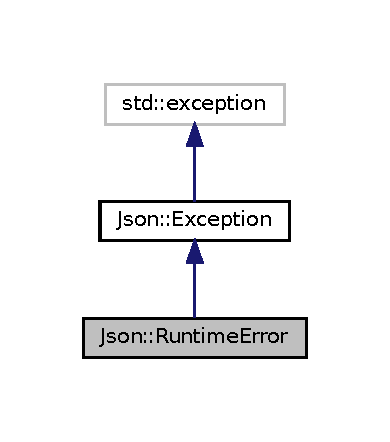
\includegraphics[width=187pt]{classJson_1_1RuntimeError__inherit__graph}
\end{center}
\end{figure}


Collaboration diagram for Json\+:\+:Runtime\+Error\+:
\nopagebreak
\begin{figure}[H]
\begin{center}
\leavevmode
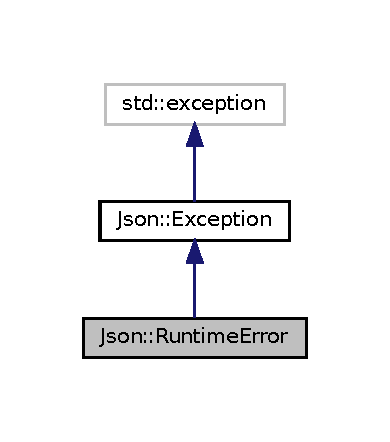
\includegraphics[width=187pt]{classJson_1_1RuntimeError__coll__graph}
\end{center}
\end{figure}
\subsection*{Public Member Functions}
\begin{DoxyCompactItemize}
\item 
\mbox{\Hypertarget{classJson_1_1RuntimeError_a0f6445dc345ce0a703610b6e893fee40}\label{classJson_1_1RuntimeError_a0f6445dc345ce0a703610b6e893fee40}} 
{\bfseries Runtime\+Error} (J\+S\+O\+N\+C\+P\+P\+\_\+\+S\+T\+R\+I\+NG const \&msg)
\end{DoxyCompactItemize}
\subsection*{Additional Inherited Members}


\subsection{Detailed Description}
Exceptions which the user cannot easily avoid.

E.\+g. out-\/of-\/memory (when we use malloc), stack-\/overflow, malicious input

\begin{DoxyRemark}{Remarks}
derived from \hyperlink{classJson_1_1Exception}{Json\+::\+Exception} 
\end{DoxyRemark}


The documentation for this class was generated from the following files\+:\begin{DoxyCompactItemize}
\item 
/home/mjonsson/repo/cpp\+Adv/media\+F\+W/inc/json/json.\+h\item 
/home/mjonsson/repo/cpp\+Adv/media\+F\+W/src/json/jsoncpp.\+cpp\end{DoxyCompactItemize}

\hypertarget{classJson_1_1StaticString}{}\section{Json\+:\+:Static\+String Class Reference}
\label{classJson_1_1StaticString}\index{Json\+::\+Static\+String@{Json\+::\+Static\+String}}


Lightweight wrapper to tag static string.  




{\ttfamily \#include $<$json.\+h$>$}

\subsection*{Public Member Functions}
\begin{DoxyCompactItemize}
\item 
\mbox{\Hypertarget{classJson_1_1StaticString_afb6baf1ec078ce76f0b0f9b39d19437f}\label{classJson_1_1StaticString_afb6baf1ec078ce76f0b0f9b39d19437f}} 
{\bfseries Static\+String} (const char $\ast$czstring)
\item 
\mbox{\Hypertarget{classJson_1_1StaticString_a256a6cc0c630aef670848a0f11707b62}\label{classJson_1_1StaticString_a256a6cc0c630aef670848a0f11707b62}} 
{\bfseries operator const char $\ast$} () const
\item 
\mbox{\Hypertarget{classJson_1_1StaticString_ad6be703d432d108623bb0aa06b0b90ca}\label{classJson_1_1StaticString_ad6be703d432d108623bb0aa06b0b90ca}} 
const char $\ast$ {\bfseries c\+\_\+str} () const
\end{DoxyCompactItemize}


\subsection{Detailed Description}
Lightweight wrapper to tag static string. 

\hyperlink{classJson_1_1Value}{Value} constructor and object\+Value member assignment takes advantage of the \hyperlink{classJson_1_1StaticString}{Static\+String} and avoid the cost of string duplication when storing the string or the member name.

Example of usage\+: 
\begin{DoxyCode}
\hyperlink{classJson_1_1Value}{Json::Value} aValue( StaticString(\textcolor{stringliteral}{"some text"}) );
\hyperlink{classJson_1_1Value}{Json::Value} object;
\textcolor{keyword}{static} \textcolor{keyword}{const} StaticString code(\textcolor{stringliteral}{"code"});
\textcolor{keywordtype}{object}[code] = 1234;
\end{DoxyCode}
 

The documentation for this class was generated from the following file\+:\begin{DoxyCompactItemize}
\item 
/home/mjonsson/repo/cpp\+Adv/media\+F\+W/inc/json/json.\+h\end{DoxyCompactItemize}

\hypertarget{classJson_1_1StreamWriter}{}\section{Json\+:\+:Stream\+Writer Class Reference}
\label{classJson_1_1StreamWriter}\index{Json\+::\+Stream\+Writer@{Json\+::\+Stream\+Writer}}


{\ttfamily \#include $<$json.\+h$>$}



Inheritance diagram for Json\+:\+:Stream\+Writer\+:
\nopagebreak
\begin{figure}[H]
\begin{center}
\leavevmode
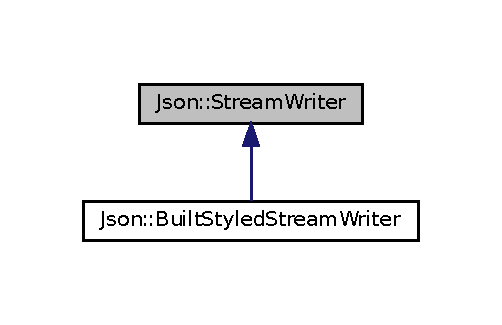
\includegraphics[width=241pt]{classJson_1_1StreamWriter__inherit__graph}
\end{center}
\end{figure}
\subsection*{Classes}
\begin{DoxyCompactItemize}
\item 
class \hyperlink{classJson_1_1StreamWriter_1_1Factory}{Factory}
\begin{DoxyCompactList}\small\item\em A simple abstract factory. \end{DoxyCompactList}\end{DoxyCompactItemize}
\subsection*{Public Member Functions}
\begin{DoxyCompactItemize}
\item 
virtual int \hyperlink{classJson_1_1StreamWriter_a84278bad0c9a9fc587bc2a97c5bb5993}{write} (\hyperlink{classJson_1_1Value}{Value} const \&root, J\+S\+O\+N\+C\+P\+P\+\_\+\+O\+S\+T\+R\+E\+AM $\ast$sout)=0
\end{DoxyCompactItemize}
\subsection*{Protected Attributes}
\begin{DoxyCompactItemize}
\item 
\mbox{\Hypertarget{classJson_1_1StreamWriter_a4f5603d4228a9fa46a42cb44e5234d9b}\label{classJson_1_1StreamWriter_a4f5603d4228a9fa46a42cb44e5234d9b}} 
J\+S\+O\+N\+C\+P\+P\+\_\+\+O\+S\+T\+R\+E\+AM $\ast$ {\bfseries sout\+\_\+}
\end{DoxyCompactItemize}


\subsection{Detailed Description}
Usage\+: 
\begin{DoxyCode}
\textcolor{keyword}{using namespace }\hyperlink{namespaceJson}{Json};
\textcolor{keywordtype}{void} writeToStdout(\hyperlink{classJson_1_1StreamWriter_1_1Factory}{StreamWriter::Factory} \textcolor{keyword}{const}& factory, 
      \hyperlink{classJson_1_1Value}{Value} \textcolor{keyword}{const}& value) \{
  std::unique\_ptr<StreamWriter> \textcolor{keyword}{const} writer(
    factory.\hyperlink{classJson_1_1StreamWriter_1_1Factory_a9d30ec53e8288cd53befccf1009c5f31}{newStreamWriter}());
  writer->write(value, &std::cout);
  std::cout << std::endl;  \textcolor{comment}{// add lf and flush}
\}
\end{DoxyCode}
 

\subsection{Member Function Documentation}
\mbox{\Hypertarget{classJson_1_1StreamWriter_a84278bad0c9a9fc587bc2a97c5bb5993}\label{classJson_1_1StreamWriter_a84278bad0c9a9fc587bc2a97c5bb5993}} 
\index{Json\+::\+Stream\+Writer@{Json\+::\+Stream\+Writer}!write@{write}}
\index{write@{write}!Json\+::\+Stream\+Writer@{Json\+::\+Stream\+Writer}}
\subsubsection{\texorpdfstring{write()}{write()}}
{\footnotesize\ttfamily virtual int Json\+::\+Stream\+Writer\+::write (\begin{DoxyParamCaption}\item[{\hyperlink{classJson_1_1Value}{Value} const \&}]{root,  }\item[{J\+S\+O\+N\+C\+P\+P\+\_\+\+O\+S\+T\+R\+E\+AM $\ast$}]{sout }\end{DoxyParamCaption})\hspace{0.3cm}{\ttfamily [pure virtual]}}

Write \hyperlink{classJson_1_1Value}{Value} into document as configured in sub-\/class. Do not take ownership of sout, but maintain a reference during function. \begin{DoxyPrecond}{Precondition}
sout != N\+U\+LL 
\end{DoxyPrecond}
\begin{DoxyReturn}{Returns}
zero on success (For now, we always return zero, so check the stream instead.) 
\end{DoxyReturn}

\begin{DoxyExceptions}{Exceptions}
{\em std\+::exception} & possibly, depending on configuration \\
\hline
\end{DoxyExceptions}


Implemented in \hyperlink{structJson_1_1BuiltStyledStreamWriter_a823cdb1afabb6b0d5f39bcd5a6a6f747}{Json\+::\+Built\+Styled\+Stream\+Writer}.



The documentation for this class was generated from the following files\+:\begin{DoxyCompactItemize}
\item 
/home/mjonsson/repo/cpp\+Adv/media\+F\+W/inc/json/json.\+h\item 
/home/mjonsson/repo/cpp\+Adv/media\+F\+W/src/json/jsoncpp.\+cpp\end{DoxyCompactItemize}

\hypertarget{classJson_1_1StreamWriterBuilder}{}\section{Json\+:\+:Stream\+Writer\+Builder Class Reference}
\label{classJson_1_1StreamWriterBuilder}\index{Json\+::\+Stream\+Writer\+Builder@{Json\+::\+Stream\+Writer\+Builder}}


Build a \hyperlink{classJson_1_1StreamWriter}{Stream\+Writer} implementation.  




{\ttfamily \#include $<$json.\+h$>$}



Inheritance diagram for Json\+:\+:Stream\+Writer\+Builder\+:
\nopagebreak
\begin{figure}[H]
\begin{center}
\leavevmode
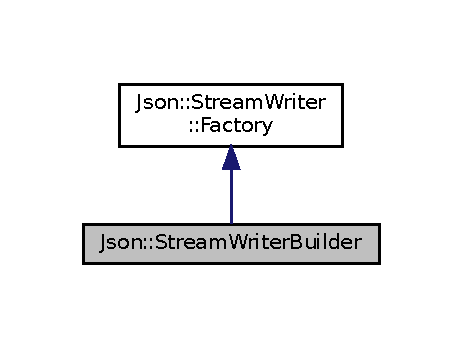
\includegraphics[width=222pt]{classJson_1_1StreamWriterBuilder__inherit__graph}
\end{center}
\end{figure}


Collaboration diagram for Json\+:\+:Stream\+Writer\+Builder\+:
\nopagebreak
\begin{figure}[H]
\begin{center}
\leavevmode
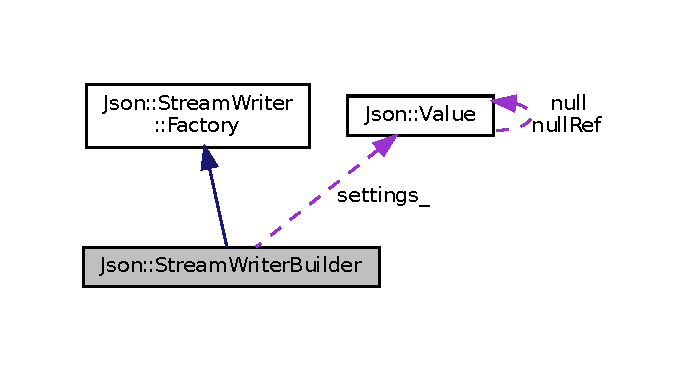
\includegraphics[width=329pt]{classJson_1_1StreamWriterBuilder__coll__graph}
\end{center}
\end{figure}
\subsection*{Public Member Functions}
\begin{DoxyCompactItemize}
\item 
\hyperlink{classJson_1_1StreamWriter}{Stream\+Writer} $\ast$ \hyperlink{classJson_1_1StreamWriterBuilder_ab9ee278609f88ae04a7c1a84e1f559e6}{new\+Stream\+Writer} () const J\+S\+O\+N\+C\+P\+P\+\_\+\+O\+V\+E\+R\+R\+I\+DE
\item 
bool \hyperlink{classJson_1_1StreamWriterBuilder_a12353b97766841db7d049da84658da09}{validate} (\hyperlink{classJson_1_1Value}{Json\+::\+Value} $\ast$invalid) const
\item 
\hyperlink{classJson_1_1Value}{Value} \& \hyperlink{classJson_1_1StreamWriterBuilder_af68f6b59cb20b074052ed12bb3d336a3}{operator\mbox{[}$\,$\mbox{]}} (J\+S\+O\+N\+C\+P\+P\+\_\+\+S\+T\+R\+I\+NG key)
\end{DoxyCompactItemize}
\subsection*{Static Public Member Functions}
\begin{DoxyCompactItemize}
\item 
static void \hyperlink{classJson_1_1StreamWriterBuilder_a53bf106b141e28637b01ad0ecd2acbf6}{set\+Defaults} (\hyperlink{classJson_1_1Value}{Json\+::\+Value} $\ast$settings)
\end{DoxyCompactItemize}
\subsection*{Public Attributes}
\begin{DoxyCompactItemize}
\item 
\hyperlink{classJson_1_1Value}{Json\+::\+Value} \hyperlink{classJson_1_1StreamWriterBuilder_a79bdf2e639a52f4e758c0b95bd1d3423}{settings\+\_\+}
\end{DoxyCompactItemize}


\subsection{Detailed Description}
Build a \hyperlink{classJson_1_1StreamWriter}{Stream\+Writer} implementation. 

Usage\+: 
\begin{DoxyCode}
\textcolor{keyword}{using namespace }\hyperlink{namespaceJson}{Json};
\hyperlink{classJson_1_1Value}{Value} value = ...;
\hyperlink{classJson_1_1StreamWriterBuilder}{StreamWriterBuilder} builder;
builder[\textcolor{stringliteral}{"commentStyle"}] = \textcolor{stringliteral}{"None"};
builder[\textcolor{stringliteral}{"indentation"}] = \textcolor{stringliteral}{"   "};  \textcolor{comment}{// or whatever you like}
std::unique\_ptr<Json::StreamWriter> writer(
    builder.\hyperlink{classJson_1_1StreamWriterBuilder_ab9ee278609f88ae04a7c1a84e1f559e6}{newStreamWriter}());
writer->write(value, &std::cout);
std::cout << std::endl;  \textcolor{comment}{// add lf and flush}
\end{DoxyCode}
 

\subsection{Member Function Documentation}
\mbox{\Hypertarget{classJson_1_1StreamWriterBuilder_ab9ee278609f88ae04a7c1a84e1f559e6}\label{classJson_1_1StreamWriterBuilder_ab9ee278609f88ae04a7c1a84e1f559e6}} 
\index{Json\+::\+Stream\+Writer\+Builder@{Json\+::\+Stream\+Writer\+Builder}!new\+Stream\+Writer@{new\+Stream\+Writer}}
\index{new\+Stream\+Writer@{new\+Stream\+Writer}!Json\+::\+Stream\+Writer\+Builder@{Json\+::\+Stream\+Writer\+Builder}}
\subsubsection{\texorpdfstring{new\+Stream\+Writer()}{newStreamWriter()}}
{\footnotesize\ttfamily \hyperlink{classJson_1_1StreamWriter}{Stream\+Writer} $\ast$ Json\+::\+Stream\+Writer\+Builder\+::new\+Stream\+Writer (\begin{DoxyParamCaption}{ }\end{DoxyParamCaption}) const\hspace{0.3cm}{\ttfamily [virtual]}}


\begin{DoxyExceptions}{Exceptions}
{\em std\+::exception} & if something goes wrong (e.\+g. invalid settings) \\
\hline
\end{DoxyExceptions}


Implements \hyperlink{classJson_1_1StreamWriter_1_1Factory_a9d30ec53e8288cd53befccf1009c5f31}{Json\+::\+Stream\+Writer\+::\+Factory}.

\mbox{\Hypertarget{classJson_1_1StreamWriterBuilder_af68f6b59cb20b074052ed12bb3d336a3}\label{classJson_1_1StreamWriterBuilder_af68f6b59cb20b074052ed12bb3d336a3}} 
\index{Json\+::\+Stream\+Writer\+Builder@{Json\+::\+Stream\+Writer\+Builder}!operator\mbox{[}\mbox{]}@{operator[]}}
\index{operator\mbox{[}\mbox{]}@{operator[]}!Json\+::\+Stream\+Writer\+Builder@{Json\+::\+Stream\+Writer\+Builder}}
\subsubsection{\texorpdfstring{operator[]()}{operator[]()}}
{\footnotesize\ttfamily \hyperlink{classJson_1_1Value}{Value} \& Json\+::\+Stream\+Writer\+Builder\+::operator\mbox{[}$\,$\mbox{]} (\begin{DoxyParamCaption}\item[{J\+S\+O\+N\+C\+P\+P\+\_\+\+S\+T\+R\+I\+NG}]{key }\end{DoxyParamCaption})}

A simple way to update a specific setting. \mbox{\Hypertarget{classJson_1_1StreamWriterBuilder_a53bf106b141e28637b01ad0ecd2acbf6}\label{classJson_1_1StreamWriterBuilder_a53bf106b141e28637b01ad0ecd2acbf6}} 
\index{Json\+::\+Stream\+Writer\+Builder@{Json\+::\+Stream\+Writer\+Builder}!set\+Defaults@{set\+Defaults}}
\index{set\+Defaults@{set\+Defaults}!Json\+::\+Stream\+Writer\+Builder@{Json\+::\+Stream\+Writer\+Builder}}
\subsubsection{\texorpdfstring{set\+Defaults()}{setDefaults()}}
{\footnotesize\ttfamily void Json\+::\+Stream\+Writer\+Builder\+::set\+Defaults (\begin{DoxyParamCaption}\item[{\hyperlink{classJson_1_1Value}{Json\+::\+Value} $\ast$}]{settings }\end{DoxyParamCaption})\hspace{0.3cm}{\ttfamily [static]}}

Called by ctor, but you can use this to reset settings\+\_\+. \begin{DoxyPrecond}{Precondition}
\textquotesingle{}settings\textquotesingle{} != N\+U\+LL (but Json\+::null is fine) 
\end{DoxyPrecond}
\begin{DoxyRemark}{Remarks}
Defaults\+: 
\begin{DoxyCodeInclude}
\end{DoxyCodeInclude}

\end{DoxyRemark}
\mbox{[}Stream\+Writer\+Builder\+Defaults\mbox{]}

\mbox{[}Stream\+Writer\+Builder\+Defaults\mbox{]} \mbox{\Hypertarget{classJson_1_1StreamWriterBuilder_a12353b97766841db7d049da84658da09}\label{classJson_1_1StreamWriterBuilder_a12353b97766841db7d049da84658da09}} 
\index{Json\+::\+Stream\+Writer\+Builder@{Json\+::\+Stream\+Writer\+Builder}!validate@{validate}}
\index{validate@{validate}!Json\+::\+Stream\+Writer\+Builder@{Json\+::\+Stream\+Writer\+Builder}}
\subsubsection{\texorpdfstring{validate()}{validate()}}
{\footnotesize\ttfamily bool Json\+::\+Stream\+Writer\+Builder\+::validate (\begin{DoxyParamCaption}\item[{\hyperlink{classJson_1_1Value}{Json\+::\+Value} $\ast$}]{invalid }\end{DoxyParamCaption}) const}

\begin{DoxyReturn}{Returns}
true if \textquotesingle{}settings\textquotesingle{} are legal and consistent; otherwise, indicate bad settings via \textquotesingle{}invalid\textquotesingle{}. 
\end{DoxyReturn}


\subsection{Member Data Documentation}
\mbox{\Hypertarget{classJson_1_1StreamWriterBuilder_a79bdf2e639a52f4e758c0b95bd1d3423}\label{classJson_1_1StreamWriterBuilder_a79bdf2e639a52f4e758c0b95bd1d3423}} 
\index{Json\+::\+Stream\+Writer\+Builder@{Json\+::\+Stream\+Writer\+Builder}!settings\+\_\+@{settings\+\_\+}}
\index{settings\+\_\+@{settings\+\_\+}!Json\+::\+Stream\+Writer\+Builder@{Json\+::\+Stream\+Writer\+Builder}}
\subsubsection{\texorpdfstring{settings\+\_\+}{settings\_}}
{\footnotesize\ttfamily \hyperlink{classJson_1_1Value}{Json\+::\+Value} Json\+::\+Stream\+Writer\+Builder\+::settings\+\_\+}

Configuration of this builder. Available settings (case-\/sensitive)\+:
\begin{DoxyItemize}
\item \char`\"{}comment\+Style\char`\"{}\+: \char`\"{}\+None\char`\"{} or \char`\"{}\+All\char`\"{}
\item \char`\"{}indentation\char`\"{}\+: \char`\"{}$<$anything$>$\char`\"{}.
\begin{DoxyItemize}
\item Setting this to an empty string also omits newline characters.
\end{DoxyItemize}
\item \char`\"{}enable\+Y\+A\+M\+L\+Compatibility\char`\"{}\+: false or true
\begin{DoxyItemize}
\item slightly change the whitespace around colons
\end{DoxyItemize}
\item \char`\"{}drop\+Null\+Placeholders\char`\"{}\+: false or true
\begin{DoxyItemize}
\item Drop the \char`\"{}null\char`\"{} string from the writer\textquotesingle{}s output for null\+Values. Strictly speaking, this is not valid J\+S\+ON. But when the output is being fed to a browser\textquotesingle{}s Java\+Script, it makes for smaller output and the browser can handle the output just fine.
\end{DoxyItemize}
\item \char`\"{}use\+Special\+Floats\char`\"{}\+: false or true
\begin{DoxyItemize}
\item If true, outputs non-\/finite floating point values in the following way\+: NaN values as \char`\"{}\+Na\+N\char`\"{}, positive infinity as \char`\"{}\+Infinity\char`\"{}, and negative infinity as \char`\"{}-\/\+Infinity\char`\"{}.
\end{DoxyItemize}
\item \char`\"{}precision\char`\"{}\+: int
\begin{DoxyItemize}
\item Number of precision digits for formatting of real values.
\end{DoxyItemize}
\item \char`\"{}precision\+Type\char`\"{}\+: \char`\"{}significant\char`\"{}(default) or \char`\"{}decimal\char`\"{}
\begin{DoxyItemize}
\item Type of precision for formatting of real values.
\end{DoxyItemize}
\end{DoxyItemize}

You can examine \textquotesingle{}settings\+\_\+` yourself to see the defaults. You can also write and read them just like any J\+S\+ON \hyperlink{classJson_1_1Value}{Value}. \begin{DoxySeeAlso}{See also}
\hyperlink{classJson_1_1StreamWriterBuilder_a53bf106b141e28637b01ad0ecd2acbf6}{set\+Defaults()} 
\end{DoxySeeAlso}


The documentation for this class was generated from the following files\+:\begin{DoxyCompactItemize}
\item 
/home/mjonsson/repo/cpp\+Adv/media\+F\+W/inc/json/json.\+h\item 
/home/mjonsson/repo/cpp\+Adv/media\+F\+W/src/jsoncpp.\+cpp\end{DoxyCompactItemize}

\hypertarget{structJson_1_1Value_1_1CZString_1_1StringStorage}{}\section{Json\+:\+:Value\+:\+:C\+Z\+String\+:\+:String\+Storage Struct Reference}
\label{structJson_1_1Value_1_1CZString_1_1StringStorage}\index{Json\+::\+Value\+::\+C\+Z\+String\+::\+String\+Storage@{Json\+::\+Value\+::\+C\+Z\+String\+::\+String\+Storage}}
\subsection*{Public Attributes}
\begin{DoxyCompactItemize}
\item 
\mbox{\Hypertarget{structJson_1_1Value_1_1CZString_1_1StringStorage_a7f68c8d6197c5692a525854b5f29f87b}\label{structJson_1_1Value_1_1CZString_1_1StringStorage_a7f68c8d6197c5692a525854b5f29f87b}} 
unsigned {\bfseries policy\+\_\+}\+: 2
\item 
\mbox{\Hypertarget{structJson_1_1Value_1_1CZString_1_1StringStorage_a165d865c44e6471d34668eeb4f15b140}\label{structJson_1_1Value_1_1CZString_1_1StringStorage_a165d865c44e6471d34668eeb4f15b140}} 
unsigned {\bfseries length\+\_\+}\+: 30
\end{DoxyCompactItemize}


The documentation for this struct was generated from the following file\+:\begin{DoxyCompactItemize}
\item 
/home/mjonsson/repo/cpp\+Adv/media\+F\+W/inc/json/json.\+h\end{DoxyCompactItemize}

\hypertarget{structJson_1_1OurReader_1_1StructuredError}{}\section{Json\+:\+:Our\+Reader\+:\+:Structured\+Error Struct Reference}
\label{structJson_1_1OurReader_1_1StructuredError}\index{Json\+::\+Our\+Reader\+::\+Structured\+Error@{Json\+::\+Our\+Reader\+::\+Structured\+Error}}
\subsection*{Public Attributes}
\begin{DoxyCompactItemize}
\item 
\mbox{\Hypertarget{structJson_1_1OurReader_1_1StructuredError_a102677698afb8177c985e72dafe72b15}\label{structJson_1_1OurReader_1_1StructuredError_a102677698afb8177c985e72dafe72b15}} 
ptrdiff\+\_\+t {\bfseries offset\+\_\+start}
\item 
\mbox{\Hypertarget{structJson_1_1OurReader_1_1StructuredError_a15491a751a39c5153af04e68b1d0abb9}\label{structJson_1_1OurReader_1_1StructuredError_a15491a751a39c5153af04e68b1d0abb9}} 
ptrdiff\+\_\+t {\bfseries offset\+\_\+limit}
\item 
\mbox{\Hypertarget{structJson_1_1OurReader_1_1StructuredError_a9d0b9986bf765d067dfcf2f971a450d1}\label{structJson_1_1OurReader_1_1StructuredError_a9d0b9986bf765d067dfcf2f971a450d1}} 
J\+S\+O\+N\+C\+P\+P\+\_\+\+S\+T\+R\+I\+NG {\bfseries message}
\end{DoxyCompactItemize}


The documentation for this struct was generated from the following file\+:\begin{DoxyCompactItemize}
\item 
/home/mjonsson/repo/cpp\+Adv/media\+F\+W/src/jsoncpp.\+cpp\end{DoxyCompactItemize}

\hypertarget{structJson_1_1Reader_1_1StructuredError}{}\section{Json\+:\+:Reader\+:\+:Structured\+Error Struct Reference}
\label{structJson_1_1Reader_1_1StructuredError}\index{Json\+::\+Reader\+::\+Structured\+Error@{Json\+::\+Reader\+::\+Structured\+Error}}


An error tagged with where in the J\+S\+ON text it was encountered.  




{\ttfamily \#include $<$json.\+h$>$}

\subsection*{Public Attributes}
\begin{DoxyCompactItemize}
\item 
\mbox{\Hypertarget{structJson_1_1Reader_1_1StructuredError_ac98af0da2d704be4b64a9572a682423b}\label{structJson_1_1Reader_1_1StructuredError_ac98af0da2d704be4b64a9572a682423b}} 
ptrdiff\+\_\+t {\bfseries offset\+\_\+start}
\item 
\mbox{\Hypertarget{structJson_1_1Reader_1_1StructuredError_ad76ac01aeb0ada7e882c2df5daa54c6e}\label{structJson_1_1Reader_1_1StructuredError_ad76ac01aeb0ada7e882c2df5daa54c6e}} 
ptrdiff\+\_\+t {\bfseries offset\+\_\+limit}
\item 
\mbox{\Hypertarget{structJson_1_1Reader_1_1StructuredError_a2d2dc387aefe406a71de3daa263a38f4}\label{structJson_1_1Reader_1_1StructuredError_a2d2dc387aefe406a71de3daa263a38f4}} 
J\+S\+O\+N\+C\+P\+P\+\_\+\+S\+T\+R\+I\+NG {\bfseries message}
\end{DoxyCompactItemize}


\subsection{Detailed Description}
An error tagged with where in the J\+S\+ON text it was encountered. 

The offsets give the \mbox{[}start, limit) range of bytes within the text. Note that this is bytes, not codepoints. 

The documentation for this struct was generated from the following file\+:\begin{DoxyCompactItemize}
\item 
/home/mjonsson/repo/cpp\+Adv/media\+F\+W/inc/json/json.\+h\end{DoxyCompactItemize}

\hypertarget{structTags}{}\section{Tags Struct Reference}
\label{structTags}\index{Tags@{Tags}}


A module representing the content of a database item.  




{\ttfamily \#include $<$Database\+Item.\+h$>$}



Collaboration diagram for Tags\+:
\nopagebreak
\begin{figure}[H]
\begin{center}
\leavevmode
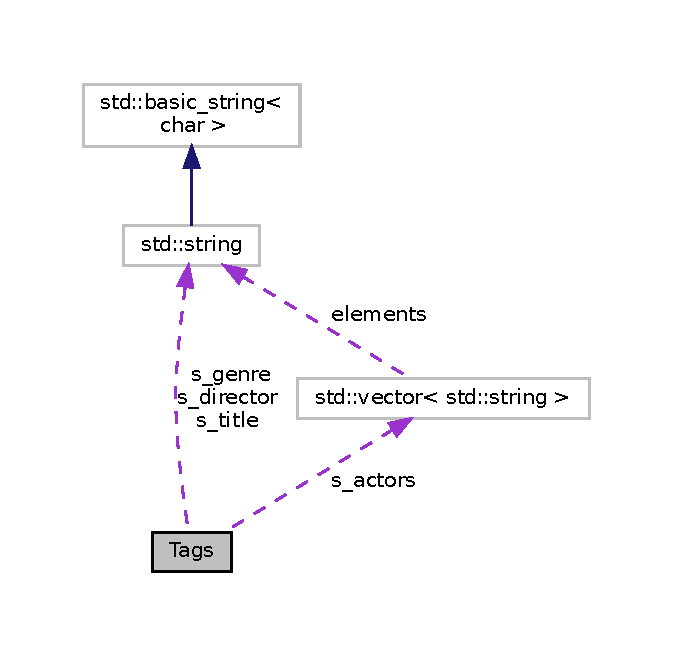
\includegraphics[width=323pt]{structTags__coll__graph}
\end{center}
\end{figure}
\subsection*{Public Attributes}
\begin{DoxyCompactItemize}
\item 
\mbox{\Hypertarget{structTags_a0af72a04b35ff5bfb11e9e602a25697c}\label{structTags_a0af72a04b35ff5bfb11e9e602a25697c}} 
std\+::string {\bfseries s\+\_\+title}
\item 
\mbox{\Hypertarget{structTags_ab983fc193a143dbd70b38a8e36f90ffb}\label{structTags_ab983fc193a143dbd70b38a8e36f90ffb}} 
std\+::string {\bfseries s\+\_\+genre}
\item 
\mbox{\Hypertarget{structTags_abd09416d0ce431b76adfc931b26738d9}\label{structTags_abd09416d0ce431b76adfc931b26738d9}} 
std\+::string {\bfseries s\+\_\+director}
\item 
\mbox{\Hypertarget{structTags_a94e73b49ee3c2acf33cc109a1411e45a}\label{structTags_a94e73b49ee3c2acf33cc109a1411e45a}} 
std\+::vector$<$ std\+::string $>$ {\bfseries s\+\_\+actors}
\end{DoxyCompactItemize}


\subsection{Detailed Description}
A module representing the content of a database item. 



The documentation for this struct was generated from the following file\+:\begin{DoxyCompactItemize}
\item 
/home/mjonsson/repo/cpp\+Adv/media\+F\+W/inc/\+Database/Database\+Item.\+h\end{DoxyCompactItemize}

\hypertarget{classJson_1_1OurReader_1_1Token}{}\section{Json\+:\+:Our\+Reader\+:\+:Token Class Reference}
\label{classJson_1_1OurReader_1_1Token}\index{Json\+::\+Our\+Reader\+::\+Token@{Json\+::\+Our\+Reader\+::\+Token}}
\subsection*{Public Attributes}
\begin{DoxyCompactItemize}
\item 
\mbox{\Hypertarget{classJson_1_1OurReader_1_1Token_abe7d858530396fa7e1293f7a579880ed}\label{classJson_1_1OurReader_1_1Token_abe7d858530396fa7e1293f7a579880ed}} 
Token\+Type {\bfseries type\+\_\+}
\item 
\mbox{\Hypertarget{classJson_1_1OurReader_1_1Token_aedf68bb00eaaa9d3c22b9825999602ac}\label{classJson_1_1OurReader_1_1Token_aedf68bb00eaaa9d3c22b9825999602ac}} 
Location {\bfseries start\+\_\+}
\item 
\mbox{\Hypertarget{classJson_1_1OurReader_1_1Token_a67d2071638add857528579ae3791eccc}\label{classJson_1_1OurReader_1_1Token_a67d2071638add857528579ae3791eccc}} 
Location {\bfseries end\+\_\+}
\end{DoxyCompactItemize}


The documentation for this class was generated from the following file\+:\begin{DoxyCompactItemize}
\item 
/home/mjonsson/repo/cpp\+Adv/media\+F\+W/src/json/jsoncpp.\+cpp\end{DoxyCompactItemize}

\hypertarget{classJson_1_1Reader_1_1Token}{}\section{Json\+:\+:Reader\+:\+:Token Class Reference}
\label{classJson_1_1Reader_1_1Token}\index{Json\+::\+Reader\+::\+Token@{Json\+::\+Reader\+::\+Token}}
\subsection*{Public Attributes}
\begin{DoxyCompactItemize}
\item 
\mbox{\Hypertarget{classJson_1_1Reader_1_1Token_aa0f06d0105ec3d8cb42427c66b991bad}\label{classJson_1_1Reader_1_1Token_aa0f06d0105ec3d8cb42427c66b991bad}} 
Token\+Type {\bfseries type\+\_\+}
\item 
\mbox{\Hypertarget{classJson_1_1Reader_1_1Token_aff87d677b9ac4b52542a00b0d6673249}\label{classJson_1_1Reader_1_1Token_aff87d677b9ac4b52542a00b0d6673249}} 
Location {\bfseries start\+\_\+}
\item 
\mbox{\Hypertarget{classJson_1_1Reader_1_1Token_a7d3bc0fa40097f435d184be4b1fd5ae1}\label{classJson_1_1Reader_1_1Token_a7d3bc0fa40097f435d184be4b1fd5ae1}} 
Location {\bfseries end\+\_\+}
\end{DoxyCompactItemize}


The documentation for this class was generated from the following file\+:\begin{DoxyCompactItemize}
\item 
/home/mjonsson/repo/cpp\+Adv/media\+F\+W/inc/json/json.\+h\end{DoxyCompactItemize}

\hypertarget{classJson_1_1Value}{}\section{Json\+:\+:Value Class Reference}
\label{classJson_1_1Value}\index{Json\+::\+Value@{Json\+::\+Value}}


Represents a \href{http://www.json.org}{\tt J\+S\+ON} value.  




{\ttfamily \#include $<$json.\+h$>$}



Collaboration diagram for Json\+:\+:Value\+:
\nopagebreak
\begin{figure}[H]
\begin{center}
\leavevmode
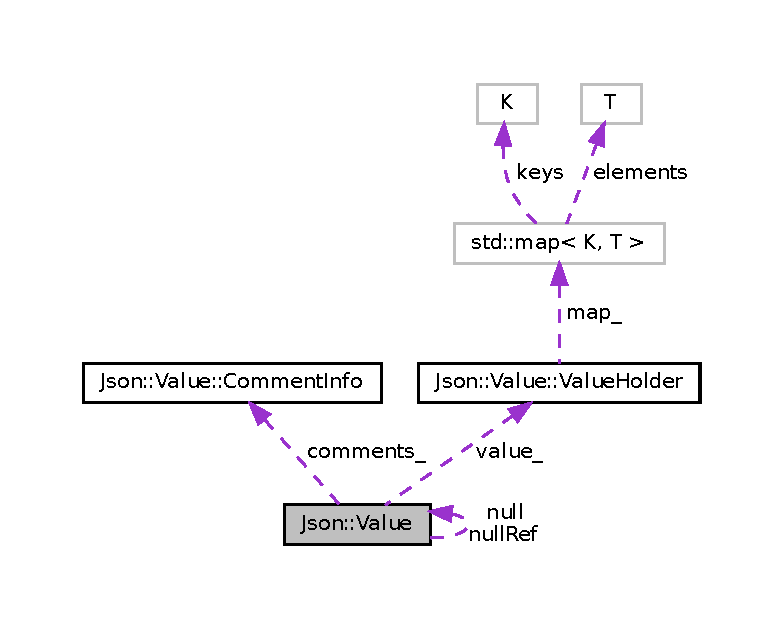
\includegraphics[width=202pt]{classJson_1_1Value__coll__graph}
\end{center}
\end{figure}
\subsection*{Public Types}
\begin{DoxyCompactItemize}
\item 
\mbox{\Hypertarget{classJson_1_1Value_a9ae9069983fc38f1928d76f9c79ac64d}\label{classJson_1_1Value_a9ae9069983fc38f1928d76f9c79ac64d}} 
typedef std\+::vector$<$ J\+S\+O\+N\+C\+P\+P\+\_\+\+S\+T\+R\+I\+NG $>$ {\bfseries Members}
\item 
\mbox{\Hypertarget{classJson_1_1Value_a341cdf2e01f8b3c5b7317aa2f0768c53}\label{classJson_1_1Value_a341cdf2e01f8b3c5b7317aa2f0768c53}} 
typedef \hyperlink{classJson_1_1ValueIterator}{Value\+Iterator} {\bfseries iterator}
\item 
\mbox{\Hypertarget{classJson_1_1Value_af92282ca92b58b320debd486afb7696a}\label{classJson_1_1Value_af92282ca92b58b320debd486afb7696a}} 
typedef \hyperlink{classJson_1_1ValueConstIterator}{Value\+Const\+Iterator} {\bfseries const\+\_\+iterator}
\item 
\mbox{\Hypertarget{classJson_1_1Value_a0933d59b45793ae4aade1757c322a98d}\label{classJson_1_1Value_a0933d59b45793ae4aade1757c322a98d}} 
typedef Json\+::\+U\+Int {\bfseries U\+Int}
\item 
\mbox{\Hypertarget{classJson_1_1Value_abdf7a7ff73eb130ffcab28504ffdb405}\label{classJson_1_1Value_abdf7a7ff73eb130ffcab28504ffdb405}} 
typedef Json\+::\+Int {\bfseries Int}
\item 
\mbox{\Hypertarget{classJson_1_1Value_a8b62564be8c087c6d18de180ff4e13e3}\label{classJson_1_1Value_a8b62564be8c087c6d18de180ff4e13e3}} 
typedef Json\+::\+U\+Int64 {\bfseries U\+Int64}
\item 
\mbox{\Hypertarget{classJson_1_1Value_a1b86af9f85f0f1baa972c3319fa22695}\label{classJson_1_1Value_a1b86af9f85f0f1baa972c3319fa22695}} 
typedef Json\+::\+Int64 {\bfseries Int64}
\item 
\mbox{\Hypertarget{classJson_1_1Value_a1cbb82642ed05109b9833e49f042ece7}\label{classJson_1_1Value_a1cbb82642ed05109b9833e49f042ece7}} 
typedef Json\+::\+Largest\+Int {\bfseries Largest\+Int}
\item 
\mbox{\Hypertarget{classJson_1_1Value_a6682a3684d635e03fc06ba229fa24eec}\label{classJson_1_1Value_a6682a3684d635e03fc06ba229fa24eec}} 
typedef Json\+::\+Largest\+U\+Int {\bfseries Largest\+U\+Int}
\item 
\mbox{\Hypertarget{classJson_1_1Value_a184a91566cccca7b819240f0d5561c7d}\label{classJson_1_1Value_a184a91566cccca7b819240f0d5561c7d}} 
typedef Json\+::\+Array\+Index {\bfseries Array\+Index}
\item 
\mbox{\Hypertarget{classJson_1_1Value_a9e071ef3c135a2c9602e893b6005d0f7}\label{classJson_1_1Value_a9e071ef3c135a2c9602e893b6005d0f7}} 
typedef std\+::string {\bfseries value\+\_\+type}
\item 
\mbox{\Hypertarget{classJson_1_1Value_a08b6c80c3af7071d908dabf044de5388}\label{classJson_1_1Value_a08b6c80c3af7071d908dabf044de5388}} 
typedef std\+::map$<$ C\+Z\+String, \hyperlink{classJson_1_1Value}{Value} $>$ {\bfseries Object\+Values}
\end{DoxyCompactItemize}
\subsection*{Public Member Functions}
\begin{DoxyCompactItemize}
\item 
\hyperlink{classJson_1_1Value_ada6ba1369448fb0240bccc36efaa46f7}{Value} (\hyperlink{namespaceJson_a7d654b75c16a57007925868e38212b4e}{Value\+Type} type=\hyperlink{namespaceJson_a7d654b75c16a57007925868e38212b4ea7d9899633b4409bd3fc107e6737f8391}{null\+Value})
\begin{DoxyCompactList}\small\item\em Create a default \hyperlink{classJson_1_1Value}{Value} of the given type. \end{DoxyCompactList}\item 
\mbox{\Hypertarget{classJson_1_1Value_a4744ae571fcf34f4b16a2257b3b3b585}\label{classJson_1_1Value_a4744ae571fcf34f4b16a2257b3b3b585}} 
{\bfseries Value} (Int value)
\item 
\mbox{\Hypertarget{classJson_1_1Value_ae67a857b01286e3499a87e95be848d20}\label{classJson_1_1Value_ae67a857b01286e3499a87e95be848d20}} 
{\bfseries Value} (U\+Int value)
\item 
\mbox{\Hypertarget{classJson_1_1Value_ab1cdc3d9a4d4cc03fa01439d43ceb1b5}\label{classJson_1_1Value_ab1cdc3d9a4d4cc03fa01439d43ceb1b5}} 
{\bfseries Value} (Int64 value)
\item 
\mbox{\Hypertarget{classJson_1_1Value_a8adda58d5ae17bf7ca6a53bab4a7b69c}\label{classJson_1_1Value_a8adda58d5ae17bf7ca6a53bab4a7b69c}} 
{\bfseries Value} (U\+Int64 value)
\item 
\mbox{\Hypertarget{classJson_1_1Value_a32228cc84d83200cca8441451997996c}\label{classJson_1_1Value_a32228cc84d83200cca8441451997996c}} 
{\bfseries Value} (double value)
\item 
\mbox{\Hypertarget{classJson_1_1Value_ad87b849356816aca75995dd07302e49d}\label{classJson_1_1Value_ad87b849356816aca75995dd07302e49d}} 
\hyperlink{classJson_1_1Value_ad87b849356816aca75995dd07302e49d}{Value} (const char $\ast$value)
\begin{DoxyCompactList}\small\item\em Copy til first 0. (N\+U\+LL causes to seg-\/fault.) \end{DoxyCompactList}\item 
\mbox{\Hypertarget{classJson_1_1Value_a39fa09d1902efbd4350e1236db920571}\label{classJson_1_1Value_a39fa09d1902efbd4350e1236db920571}} 
\hyperlink{classJson_1_1Value_a39fa09d1902efbd4350e1236db920571}{Value} (const char $\ast$begin, const char $\ast$end)
\begin{DoxyCompactList}\small\item\em Copy all, incl zeroes. \end{DoxyCompactList}\item 
\hyperlink{classJson_1_1Value_a081830e95f88a37054da7e46c65b0766}{Value} (const \hyperlink{classJson_1_1StaticString}{Static\+String} \&value)
\begin{DoxyCompactList}\small\item\em Constructs a value from a static string. \end{DoxyCompactList}\item 
\hyperlink{classJson_1_1Value_a89ef37969ff7c6eb3a7afcca03d4cd4a}{Value} (const J\+S\+O\+N\+C\+P\+P\+\_\+\+S\+T\+R\+I\+NG \&value)
\item 
\mbox{\Hypertarget{classJson_1_1Value_a350a31ea4a30d384994b0bc010b17495}\label{classJson_1_1Value_a350a31ea4a30d384994b0bc010b17495}} 
{\bfseries Value} (bool value)
\item 
\mbox{\Hypertarget{classJson_1_1Value_a436dfd3670f95fd665f680eba5cebcf0}\label{classJson_1_1Value_a436dfd3670f95fd665f680eba5cebcf0}} 
\hyperlink{classJson_1_1Value_a436dfd3670f95fd665f680eba5cebcf0}{Value} (const \hyperlink{classJson_1_1Value}{Value} \&other)
\begin{DoxyCompactList}\small\item\em Deep copy. \end{DoxyCompactList}\item 
\hyperlink{classJson_1_1Value}{Value} \& \hyperlink{classJson_1_1Value_a795acb28772da4c5d85ae8f4af36c69f}{operator=} (\hyperlink{classJson_1_1Value}{Value} other)
\item 
\mbox{\Hypertarget{classJson_1_1Value_aab841120d78e296e1bc06a373345e822}\label{classJson_1_1Value_aab841120d78e296e1bc06a373345e822}} 
void \hyperlink{classJson_1_1Value_aab841120d78e296e1bc06a373345e822}{swap} (\hyperlink{classJson_1_1Value}{Value} \&other)
\begin{DoxyCompactList}\small\item\em Swap everything. \end{DoxyCompactList}\item 
\mbox{\Hypertarget{classJson_1_1Value_a5263476047f20e2fc6de470e4de34fe5}\label{classJson_1_1Value_a5263476047f20e2fc6de470e4de34fe5}} 
void \hyperlink{classJson_1_1Value_a5263476047f20e2fc6de470e4de34fe5}{swap\+Payload} (\hyperlink{classJson_1_1Value}{Value} \&other)
\begin{DoxyCompactList}\small\item\em Swap values but leave comments and source offsets in place. \end{DoxyCompactList}\item 
\mbox{\Hypertarget{classJson_1_1Value_a1b2c6379664d91b9f1bcd4d1853e5970}\label{classJson_1_1Value_a1b2c6379664d91b9f1bcd4d1853e5970}} 
void \hyperlink{classJson_1_1Value_a1b2c6379664d91b9f1bcd4d1853e5970}{copy} (const \hyperlink{classJson_1_1Value}{Value} \&other)
\begin{DoxyCompactList}\small\item\em copy everything. \end{DoxyCompactList}\item 
\mbox{\Hypertarget{classJson_1_1Value_ab504d299cfaa440392037fa8a3c54064}\label{classJson_1_1Value_ab504d299cfaa440392037fa8a3c54064}} 
void \hyperlink{classJson_1_1Value_ab504d299cfaa440392037fa8a3c54064}{copy\+Payload} (const \hyperlink{classJson_1_1Value}{Value} \&other)
\begin{DoxyCompactList}\small\item\em copy values but leave comments and source offsets in place. \end{DoxyCompactList}\item 
\mbox{\Hypertarget{classJson_1_1Value_a8ce61157a011894f0252ceed232312de}\label{classJson_1_1Value_a8ce61157a011894f0252ceed232312de}} 
\hyperlink{namespaceJson_a7d654b75c16a57007925868e38212b4e}{Value\+Type} {\bfseries type} () const
\item 
\mbox{\Hypertarget{classJson_1_1Value_aac6bd14155b88ed2d39ef54820b39e49}\label{classJson_1_1Value_aac6bd14155b88ed2d39ef54820b39e49}} 
bool \hyperlink{classJson_1_1Value_aac6bd14155b88ed2d39ef54820b39e49}{operator$<$} (const \hyperlink{classJson_1_1Value}{Value} \&other) const
\begin{DoxyCompactList}\small\item\em Compare payload only, not comments etc. \end{DoxyCompactList}\item 
\mbox{\Hypertarget{classJson_1_1Value_a40c411a320a416d5eac0052b36211286}\label{classJson_1_1Value_a40c411a320a416d5eac0052b36211286}} 
bool {\bfseries operator$<$=} (const \hyperlink{classJson_1_1Value}{Value} \&other) const
\item 
\mbox{\Hypertarget{classJson_1_1Value_afe2c3e52df60b9622cbd8358b74bdbf5}\label{classJson_1_1Value_afe2c3e52df60b9622cbd8358b74bdbf5}} 
bool {\bfseries operator$>$=} (const \hyperlink{classJson_1_1Value}{Value} \&other) const
\item 
\mbox{\Hypertarget{classJson_1_1Value_a4646c2f0764908c0972160c7c2ebe567}\label{classJson_1_1Value_a4646c2f0764908c0972160c7c2ebe567}} 
bool {\bfseries operator$>$} (const \hyperlink{classJson_1_1Value}{Value} \&other) const
\item 
\mbox{\Hypertarget{classJson_1_1Value_a16f9250e30d5c4505cd11137c564a764}\label{classJson_1_1Value_a16f9250e30d5c4505cd11137c564a764}} 
bool {\bfseries operator==} (const \hyperlink{classJson_1_1Value}{Value} \&other) const
\item 
\mbox{\Hypertarget{classJson_1_1Value_a86e95be072e515c48abc61dec63a1689}\label{classJson_1_1Value_a86e95be072e515c48abc61dec63a1689}} 
bool {\bfseries operator!=} (const \hyperlink{classJson_1_1Value}{Value} \&other) const
\item 
\mbox{\Hypertarget{classJson_1_1Value_aefa4464ca1bb0bcc9a87b38ed62ca2e0}\label{classJson_1_1Value_aefa4464ca1bb0bcc9a87b38ed62ca2e0}} 
int {\bfseries compare} (const \hyperlink{classJson_1_1Value}{Value} \&other) const
\item 
\mbox{\Hypertarget{classJson_1_1Value_a16668c8db7ef0a5de040012f0dfd84b0}\label{classJson_1_1Value_a16668c8db7ef0a5de040012f0dfd84b0}} 
const char $\ast$ \hyperlink{classJson_1_1Value_a16668c8db7ef0a5de040012f0dfd84b0}{as\+C\+String} () const
\begin{DoxyCompactList}\small\item\em Embedded zeroes could cause you trouble! \end{DoxyCompactList}\item 
\mbox{\Hypertarget{classJson_1_1Value_ae3f9b0d38f820ccdd8888aa92ea6e792}\label{classJson_1_1Value_ae3f9b0d38f820ccdd8888aa92ea6e792}} 
J\+S\+O\+N\+C\+P\+P\+\_\+\+S\+T\+R\+I\+NG \hyperlink{classJson_1_1Value_ae3f9b0d38f820ccdd8888aa92ea6e792}{as\+String} () const
\begin{DoxyCompactList}\small\item\em Embedded zeroes are possible. \end{DoxyCompactList}\item 
bool \hyperlink{classJson_1_1Value_a2e1b7be6bde2fe23f15290d9ddbbdf8a}{get\+String} (char const $\ast$$\ast$begin, char const $\ast$$\ast$end) const
\item 
\mbox{\Hypertarget{classJson_1_1Value_a614d635bc248a592593feb322cd15ab8}\label{classJson_1_1Value_a614d635bc248a592593feb322cd15ab8}} 
Int {\bfseries as\+Int} () const
\item 
\mbox{\Hypertarget{classJson_1_1Value_a74b305583ec3aacf4f9dd06e799dc265}\label{classJson_1_1Value_a74b305583ec3aacf4f9dd06e799dc265}} 
U\+Int {\bfseries as\+U\+Int} () const
\item 
\mbox{\Hypertarget{classJson_1_1Value_af7371262e51d5c564908f5aa684516d1}\label{classJson_1_1Value_af7371262e51d5c564908f5aa684516d1}} 
Int64 {\bfseries as\+Int64} () const
\item 
\mbox{\Hypertarget{classJson_1_1Value_aca53fe8b4bdd385010d431e5d01b3987}\label{classJson_1_1Value_aca53fe8b4bdd385010d431e5d01b3987}} 
U\+Int64 {\bfseries as\+U\+Int64} () const
\item 
\mbox{\Hypertarget{classJson_1_1Value_ab16f2ea2a117a1b3b576acab8b6a700d}\label{classJson_1_1Value_ab16f2ea2a117a1b3b576acab8b6a700d}} 
Largest\+Int {\bfseries as\+Largest\+Int} () const
\item 
\mbox{\Hypertarget{classJson_1_1Value_ad03548101e0bf3d2d9eac75c64a0b8d7}\label{classJson_1_1Value_ad03548101e0bf3d2d9eac75c64a0b8d7}} 
Largest\+U\+Int {\bfseries as\+Largest\+U\+Int} () const
\item 
\mbox{\Hypertarget{classJson_1_1Value_af3a4d10bf575fabdc5440a7135c9649c}\label{classJson_1_1Value_af3a4d10bf575fabdc5440a7135c9649c}} 
float {\bfseries as\+Float} () const
\item 
\mbox{\Hypertarget{classJson_1_1Value_afd24002a18aef907ad746b1cb9eda0a2}\label{classJson_1_1Value_afd24002a18aef907ad746b1cb9eda0a2}} 
double {\bfseries as\+Double} () const
\item 
\mbox{\Hypertarget{classJson_1_1Value_ab693fb7b9b1595bb0adc49658bbf780d}\label{classJson_1_1Value_ab693fb7b9b1595bb0adc49658bbf780d}} 
bool {\bfseries as\+Bool} () const
\item 
\mbox{\Hypertarget{classJson_1_1Value_abde4070e21e46dc4f8203f66582cb19f}\label{classJson_1_1Value_abde4070e21e46dc4f8203f66582cb19f}} 
bool {\bfseries is\+Null} () const
\item 
\mbox{\Hypertarget{classJson_1_1Value_ab1f02651cb89d0f18b63a036959391ba}\label{classJson_1_1Value_ab1f02651cb89d0f18b63a036959391ba}} 
bool {\bfseries is\+Bool} () const
\item 
\mbox{\Hypertarget{classJson_1_1Value_aff51d8b52979ca06cf9d909accd5f695}\label{classJson_1_1Value_aff51d8b52979ca06cf9d909accd5f695}} 
bool {\bfseries is\+Int} () const
\item 
\mbox{\Hypertarget{classJson_1_1Value_a4a81fb3c3acdbb68b2e2f30836a4f53e}\label{classJson_1_1Value_a4a81fb3c3acdbb68b2e2f30836a4f53e}} 
bool {\bfseries is\+Int64} () const
\item 
\mbox{\Hypertarget{classJson_1_1Value_abdda463d3269015f883587349726cfbc}\label{classJson_1_1Value_abdda463d3269015f883587349726cfbc}} 
bool {\bfseries is\+U\+Int} () const
\item 
\mbox{\Hypertarget{classJson_1_1Value_a883576e35cb03a785258edb56777a2de}\label{classJson_1_1Value_a883576e35cb03a785258edb56777a2de}} 
bool {\bfseries is\+U\+Int64} () const
\item 
\mbox{\Hypertarget{classJson_1_1Value_ab6798954f6e80281cf22708ef45198a7}\label{classJson_1_1Value_ab6798954f6e80281cf22708ef45198a7}} 
bool {\bfseries is\+Integral} () const
\item 
\mbox{\Hypertarget{classJson_1_1Value_a4a2e2a790e19a1c09fc5dd12d7ad47b5}\label{classJson_1_1Value_a4a2e2a790e19a1c09fc5dd12d7ad47b5}} 
bool {\bfseries is\+Double} () const
\item 
\mbox{\Hypertarget{classJson_1_1Value_af961a000cd203c895e44c195ab39b866}\label{classJson_1_1Value_af961a000cd203c895e44c195ab39b866}} 
bool {\bfseries is\+Numeric} () const
\item 
\mbox{\Hypertarget{classJson_1_1Value_a71e1f82cf1c3eaf969d400dcffb163a6}\label{classJson_1_1Value_a71e1f82cf1c3eaf969d400dcffb163a6}} 
bool {\bfseries is\+String} () const
\item 
\mbox{\Hypertarget{classJson_1_1Value_a1627eb9d6568d6d0252fa8bb711c0a59}\label{classJson_1_1Value_a1627eb9d6568d6d0252fa8bb711c0a59}} 
bool {\bfseries is\+Array} () const
\item 
\mbox{\Hypertarget{classJson_1_1Value_a8cf96c0f2a552051fcfc78ffee60e037}\label{classJson_1_1Value_a8cf96c0f2a552051fcfc78ffee60e037}} 
bool {\bfseries is\+Object} () const
\item 
\mbox{\Hypertarget{classJson_1_1Value_af1ee6be27a96a7d12128efdd60deb54d}\label{classJson_1_1Value_af1ee6be27a96a7d12128efdd60deb54d}} 
bool {\bfseries is\+Convertible\+To} (\hyperlink{namespaceJson_a7d654b75c16a57007925868e38212b4e}{Value\+Type} other) const
\item 
\mbox{\Hypertarget{classJson_1_1Value_a0ec2808e1d7efa4e9fad938d6667be44}\label{classJson_1_1Value_a0ec2808e1d7efa4e9fad938d6667be44}} 
Array\+Index \hyperlink{classJson_1_1Value_a0ec2808e1d7efa4e9fad938d6667be44}{size} () const
\begin{DoxyCompactList}\small\item\em Number of values in array or object. \end{DoxyCompactList}\item 
\mbox{\Hypertarget{classJson_1_1Value_a0519a551e37ee6665d74742b3f96bab3}\label{classJson_1_1Value_a0519a551e37ee6665d74742b3f96bab3}} 
bool \hyperlink{classJson_1_1Value_a0519a551e37ee6665d74742b3f96bab3}{empty} () const
\begin{DoxyCompactList}\small\item\em Return true if empty array, empty object, or null; otherwise, false. \end{DoxyCompactList}\item 
\mbox{\Hypertarget{classJson_1_1Value_a2addc2bcedbd6f8a1eafa49e9adcc729}\label{classJson_1_1Value_a2addc2bcedbd6f8a1eafa49e9adcc729}} 
J\+S\+O\+N\+C\+P\+P\+\_\+\+O\+P\+\_\+\+E\+X\+P\+L\+I\+C\+IT \hyperlink{classJson_1_1Value_a2addc2bcedbd6f8a1eafa49e9adcc729}{operator bool} () const
\begin{DoxyCompactList}\small\item\em Return !is\+Null() \end{DoxyCompactList}\item 
void \hyperlink{classJson_1_1Value_a501a4d67e6c875255c2ecc03ccd2019b}{clear} ()
\item 
void \hyperlink{classJson_1_1Value_a7a064d8aa47fde09a268be2aea992134}{resize} (Array\+Index new\+Size)
\item 
\hyperlink{classJson_1_1Value}{Value} \& \hyperlink{classJson_1_1Value_a7d99f5dba388cdaa152ce6ef933d64ef}{operator\mbox{[}$\,$\mbox{]}} (Array\+Index index)
\item 
\hyperlink{classJson_1_1Value}{Value} \& \hyperlink{classJson_1_1Value_ac9182982c361e0ab621134d406e5f250}{operator\mbox{[}$\,$\mbox{]}} (int index)
\item 
const \hyperlink{classJson_1_1Value}{Value} \& \hyperlink{classJson_1_1Value_a46607236038b29695ed80c15895271e4}{operator\mbox{[}$\,$\mbox{]}} (Array\+Index index) const
\item 
const \hyperlink{classJson_1_1Value}{Value} \& \hyperlink{classJson_1_1Value_a0b42557a95621a4676b46a21ffc5e949}{operator\mbox{[}$\,$\mbox{]}} (int index) const
\item 
\hyperlink{classJson_1_1Value}{Value} \hyperlink{classJson_1_1Value_a034eb7bf85a44fa759bdaa232788ca66}{get} (Array\+Index index, const \hyperlink{classJson_1_1Value}{Value} \&default\+Value) const
\item 
\mbox{\Hypertarget{classJson_1_1Value_ac2928f174a6e081c1500c28c2d61ee93}\label{classJson_1_1Value_ac2928f174a6e081c1500c28c2d61ee93}} 
bool \hyperlink{classJson_1_1Value_ac2928f174a6e081c1500c28c2d61ee93}{is\+Valid\+Index} (Array\+Index index) const
\begin{DoxyCompactList}\small\item\em Return true if index $<$ \hyperlink{classJson_1_1Value_a0ec2808e1d7efa4e9fad938d6667be44}{size()}. \end{DoxyCompactList}\item 
\hyperlink{classJson_1_1Value}{Value} \& \hyperlink{classJson_1_1Value_a7e49ac977e4bcf59745a09d426669f75}{append} (const \hyperlink{classJson_1_1Value}{Value} \&value)
\begin{DoxyCompactList}\small\item\em Append value to array at the end. \end{DoxyCompactList}\item 
\hyperlink{classJson_1_1Value}{Value} \& \hyperlink{classJson_1_1Value_acb912f4ec40a25ea6eb387730885f3d9}{operator\mbox{[}$\,$\mbox{]}} (const char $\ast$key)
\item 
const \hyperlink{classJson_1_1Value}{Value} \& \hyperlink{classJson_1_1Value_a1b0498b7b2a520a68137f682d91abdd5}{operator\mbox{[}$\,$\mbox{]}} (const char $\ast$key) const
\item 
\hyperlink{classJson_1_1Value}{Value} \& \hyperlink{classJson_1_1Value_aedd1e152756a4cc8c1ebac0dd7aeeb78}{operator\mbox{[}$\,$\mbox{]}} (const J\+S\+O\+N\+C\+P\+P\+\_\+\+S\+T\+R\+I\+NG \&key)
\item 
const \hyperlink{classJson_1_1Value}{Value} \& \hyperlink{classJson_1_1Value_aba60f69dcd85e935aa85e7a517e03427}{operator\mbox{[}$\,$\mbox{]}} (const J\+S\+O\+N\+C\+P\+P\+\_\+\+S\+T\+R\+I\+NG \&key) const
\item 
\hyperlink{classJson_1_1Value}{Value} \& \hyperlink{classJson_1_1Value_ac3763d7d315ca65dc188e273722f7955}{operator\mbox{[}$\,$\mbox{]}} (const \hyperlink{classJson_1_1StaticString}{Static\+String} \&key)
\begin{DoxyCompactList}\small\item\em Access an object value by name, create a null member if it does not exist. \end{DoxyCompactList}\item 
\hyperlink{classJson_1_1Value}{Value} \hyperlink{classJson_1_1Value_a57de86629ed23246f14014fb6c44fa67}{get} (const char $\ast$key, const \hyperlink{classJson_1_1Value}{Value} \&default\+Value) const
\item 
\hyperlink{classJson_1_1Value}{Value} \hyperlink{classJson_1_1Value_aa59ed050e87e1d58d93671a38687f36c}{get} (const char $\ast$begin, const char $\ast$end, const \hyperlink{classJson_1_1Value}{Value} \&default\+Value) const
\item 
\hyperlink{classJson_1_1Value}{Value} \hyperlink{classJson_1_1Value_a7406e6af727c288bf8ab59945ece686a}{get} (const J\+S\+O\+N\+C\+P\+P\+\_\+\+S\+T\+R\+I\+NG \&key, const \hyperlink{classJson_1_1Value}{Value} \&default\+Value) const
\item 
\hyperlink{classJson_1_1Value}{Value} const  $\ast$ \hyperlink{classJson_1_1Value_afb007b9ce9b2cf9d5f667a07e5e0349f}{find} (char const $\ast$begin, char const $\ast$end) const
\item 
\hyperlink{classJson_1_1Value}{Value} const  $\ast$ \hyperlink{classJson_1_1Value_afeb7ff596a0929d90c5f2f3cffb413ed}{demand} (char const $\ast$begin, char const $\ast$end)
\item 
void \hyperlink{classJson_1_1Value_a92e165f04105d27a930fb3a18a053585}{remove\+Member} (const char $\ast$key)
\begin{DoxyCompactList}\small\item\em Remove and return the named member. \end{DoxyCompactList}\item 
void \hyperlink{classJson_1_1Value_a8a660202bbad35857b39e85bd35ec78a}{remove\+Member} (const J\+S\+O\+N\+C\+P\+P\+\_\+\+S\+T\+R\+I\+NG \&key)
\item 
bool \hyperlink{classJson_1_1Value_a708e599489adf30d65bf85a8ee16e6fb}{remove\+Member} (const char $\ast$key, \hyperlink{classJson_1_1Value}{Value} $\ast$removed)
\item 
bool \hyperlink{classJson_1_1Value_ae385ecef98427970df525ee876e9f54a}{remove\+Member} (J\+S\+O\+N\+C\+P\+P\+\_\+\+S\+T\+R\+I\+NG const \&key, \hyperlink{classJson_1_1Value}{Value} $\ast$removed)
\begin{DoxyCompactList}\small\item\em Remove the named map member. \end{DoxyCompactList}\item 
\mbox{\Hypertarget{classJson_1_1Value_a49c91af727d6b4eb0af02a81bb2def87}\label{classJson_1_1Value_a49c91af727d6b4eb0af02a81bb2def87}} 
bool \hyperlink{classJson_1_1Value_a49c91af727d6b4eb0af02a81bb2def87}{remove\+Member} (const char $\ast$begin, const char $\ast$end, \hyperlink{classJson_1_1Value}{Value} $\ast$removed)
\begin{DoxyCompactList}\small\item\em Same as \hyperlink{classJson_1_1Value_ae385ecef98427970df525ee876e9f54a}{remove\+Member(\+J\+S\+O\+N\+C\+P\+P\+\_\+\+S\+T\+R\+I\+N\+G const\& key, Value$\ast$ removed)} \end{DoxyCompactList}\item 
bool \hyperlink{classJson_1_1Value_a64160c23c1f2f8b33913364f25d6c58d}{remove\+Index} (Array\+Index index, \hyperlink{classJson_1_1Value}{Value} $\ast$removed)
\begin{DoxyCompactList}\small\item\em Remove the indexed array element. \end{DoxyCompactList}\item 
bool \hyperlink{classJson_1_1Value_ad6d4df2227321bab05e86667609a7fad}{is\+Member} (const char $\ast$key) const
\item 
bool \hyperlink{classJson_1_1Value_a0c2cd838217b23ee6bde8135de1b30d9}{is\+Member} (const J\+S\+O\+N\+C\+P\+P\+\_\+\+S\+T\+R\+I\+NG \&key) const
\item 
\mbox{\Hypertarget{classJson_1_1Value_a2007e1e51f21f44ecf1f13e4a1c567b9}\label{classJson_1_1Value_a2007e1e51f21f44ecf1f13e4a1c567b9}} 
bool \hyperlink{classJson_1_1Value_a2007e1e51f21f44ecf1f13e4a1c567b9}{is\+Member} (const char $\ast$begin, const char $\ast$end) const
\begin{DoxyCompactList}\small\item\em Same as \hyperlink{classJson_1_1Value_a0c2cd838217b23ee6bde8135de1b30d9}{is\+Member(\+J\+S\+O\+N\+C\+P\+P\+\_\+\+S\+T\+R\+I\+N\+G const\& key)const}. \end{DoxyCompactList}\item 
Members \hyperlink{classJson_1_1Value_a79d7725dce6260317333e69022367ac9}{get\+Member\+Names} () const
\begin{DoxyCompactList}\small\item\em Return a list of the member names. \end{DoxyCompactList}\item 
void \hyperlink{classJson_1_1Value_a29f3a30f7e5d3af6f38d57999bf5b480}{set\+Comment} (const char $\ast$comment, \hyperlink{namespaceJson_a4fc417c23905b2ae9e2c47d197a45351}{Comment\+Placement} placement)
\item 
\mbox{\Hypertarget{classJson_1_1Value_a2900152a2887b410a9ddabe278b9d492}\label{classJson_1_1Value_a2900152a2887b410a9ddabe278b9d492}} 
void \hyperlink{classJson_1_1Value_a2900152a2887b410a9ddabe278b9d492}{set\+Comment} (const char $\ast$comment, size\+\_\+t len, \hyperlink{namespaceJson_a4fc417c23905b2ae9e2c47d197a45351}{Comment\+Placement} placement)
\begin{DoxyCompactList}\small\item\em Comments must be //... or /$\ast$ ... $\ast$/. \end{DoxyCompactList}\item 
\mbox{\Hypertarget{classJson_1_1Value_a2c5d13a5f45eb77e912008778e65b27f}\label{classJson_1_1Value_a2c5d13a5f45eb77e912008778e65b27f}} 
void \hyperlink{classJson_1_1Value_a2c5d13a5f45eb77e912008778e65b27f}{set\+Comment} (const J\+S\+O\+N\+C\+P\+P\+\_\+\+S\+T\+R\+I\+NG \&comment, \hyperlink{namespaceJson_a4fc417c23905b2ae9e2c47d197a45351}{Comment\+Placement} placement)
\begin{DoxyCompactList}\small\item\em Comments must be //... or /$\ast$ ... $\ast$/. \end{DoxyCompactList}\item 
\mbox{\Hypertarget{classJson_1_1Value_a65d8e3ab6a5871cbd019a3e0f0b944a3}\label{classJson_1_1Value_a65d8e3ab6a5871cbd019a3e0f0b944a3}} 
bool {\bfseries has\+Comment} (\hyperlink{namespaceJson_a4fc417c23905b2ae9e2c47d197a45351}{Comment\+Placement} placement) const
\item 
\mbox{\Hypertarget{classJson_1_1Value_a82817229a986f0b254e31d5c83066ffe}\label{classJson_1_1Value_a82817229a986f0b254e31d5c83066ffe}} 
J\+S\+O\+N\+C\+P\+P\+\_\+\+S\+T\+R\+I\+NG \hyperlink{classJson_1_1Value_a82817229a986f0b254e31d5c83066ffe}{get\+Comment} (\hyperlink{namespaceJson_a4fc417c23905b2ae9e2c47d197a45351}{Comment\+Placement} placement) const
\begin{DoxyCompactList}\small\item\em Include delimiters and embedded newlines. \end{DoxyCompactList}\item 
\mbox{\Hypertarget{classJson_1_1Value_a00154cc8662d7a845ed59e175c2496cb}\label{classJson_1_1Value_a00154cc8662d7a845ed59e175c2496cb}} 
J\+S\+O\+N\+C\+P\+P\+\_\+\+S\+T\+R\+I\+NG {\bfseries to\+Styled\+String} () const
\item 
\mbox{\Hypertarget{classJson_1_1Value_a015459a3950c198d63a2d3be8f5ae296}\label{classJson_1_1Value_a015459a3950c198d63a2d3be8f5ae296}} 
\hyperlink{classJson_1_1ValueConstIterator}{const\+\_\+iterator} {\bfseries begin} () const
\item 
\mbox{\Hypertarget{classJson_1_1Value_a3e443cd0ef24f7e028b175e47ee045e0}\label{classJson_1_1Value_a3e443cd0ef24f7e028b175e47ee045e0}} 
\hyperlink{classJson_1_1ValueConstIterator}{const\+\_\+iterator} {\bfseries end} () const
\item 
\mbox{\Hypertarget{classJson_1_1Value_a2d45bb2e68e8f22fe356d7d955ebd3c9}\label{classJson_1_1Value_a2d45bb2e68e8f22fe356d7d955ebd3c9}} 
\hyperlink{classJson_1_1ValueIterator}{iterator} {\bfseries begin} ()
\item 
\mbox{\Hypertarget{classJson_1_1Value_a2f961eff73f7f79cd29260b6cbd42558}\label{classJson_1_1Value_a2f961eff73f7f79cd29260b6cbd42558}} 
\hyperlink{classJson_1_1ValueIterator}{iterator} {\bfseries end} ()
\item 
\mbox{\Hypertarget{classJson_1_1Value_a92e32ea0f4f8a15853a3cf0beac9feb9}\label{classJson_1_1Value_a92e32ea0f4f8a15853a3cf0beac9feb9}} 
void {\bfseries set\+Offset\+Start} (ptrdiff\+\_\+t start)
\item 
\mbox{\Hypertarget{classJson_1_1Value_a5e4f5853fec138150c5df6004a8c2bcf}\label{classJson_1_1Value_a5e4f5853fec138150c5df6004a8c2bcf}} 
void {\bfseries set\+Offset\+Limit} (ptrdiff\+\_\+t limit)
\item 
\mbox{\Hypertarget{classJson_1_1Value_afa081dc764000951a1d8d6148155508e}\label{classJson_1_1Value_afa081dc764000951a1d8d6148155508e}} 
ptrdiff\+\_\+t {\bfseries get\+Offset\+Start} () const
\item 
\mbox{\Hypertarget{classJson_1_1Value_a2cdfa01935f87fcace90d450cbd2c0a4}\label{classJson_1_1Value_a2cdfa01935f87fcace90d450cbd2c0a4}} 
ptrdiff\+\_\+t {\bfseries get\+Offset\+Limit} () const
\end{DoxyCompactItemize}
\subsection*{Static Public Member Functions}
\begin{DoxyCompactItemize}
\item 
\mbox{\Hypertarget{classJson_1_1Value_af2f124567acc35d021a424e53ebdfcab}\label{classJson_1_1Value_af2f124567acc35d021a424e53ebdfcab}} 
static \hyperlink{classJson_1_1Value}{Value} const  \& \hyperlink{classJson_1_1Value_af2f124567acc35d021a424e53ebdfcab}{null\+Singleton} ()
\begin{DoxyCompactList}\small\item\em Prefer this to null or null\+Ref. \end{DoxyCompactList}\end{DoxyCompactItemize}
\subsection*{Static Public Attributes}
\begin{DoxyCompactItemize}
\item 
static const \hyperlink{classJson_1_1Value}{Value} \& \hyperlink{classJson_1_1Value_a21ddb05b92c60c7548e928bf371e7d45}{null} = \hyperlink{classJson_1_1Value_af2f124567acc35d021a424e53ebdfcab}{Value\+::null\+Singleton}()
\item 
static const \hyperlink{classJson_1_1Value}{Value} \& \hyperlink{classJson_1_1Value_aaee27e622f87266f861216d644603730}{null\+Ref} = \hyperlink{classJson_1_1Value_af2f124567acc35d021a424e53ebdfcab}{Value\+::null\+Singleton}()
\item 
\mbox{\Hypertarget{classJson_1_1Value_af91df130daa50dd43d2cd89e6ee67706}\label{classJson_1_1Value_af91df130daa50dd43d2cd89e6ee67706}} 
static const Largest\+Int \hyperlink{classJson_1_1Value_af91df130daa50dd43d2cd89e6ee67706}{min\+Largest\+Int} = Largest\+Int($\sim$(Largest\+U\+Int(-\/1) / 2))
\begin{DoxyCompactList}\small\item\em Minimum signed integer value that can be stored in a \hyperlink{classJson_1_1Value}{Json\+::\+Value}. \end{DoxyCompactList}\item 
\mbox{\Hypertarget{classJson_1_1Value_a8b4977696f13296fa8755c7953fafb2f}\label{classJson_1_1Value_a8b4977696f13296fa8755c7953fafb2f}} 
static const Largest\+Int \hyperlink{classJson_1_1Value_a8b4977696f13296fa8755c7953fafb2f}{max\+Largest\+Int} = Largest\+Int(Largest\+U\+Int(-\/1) / 2)
\begin{DoxyCompactList}\small\item\em Maximum signed integer value that can be stored in a \hyperlink{classJson_1_1Value}{Json\+::\+Value}. \end{DoxyCompactList}\item 
\mbox{\Hypertarget{classJson_1_1Value_a8ddb32d9d55fa5323ae5135639dc2e31}\label{classJson_1_1Value_a8ddb32d9d55fa5323ae5135639dc2e31}} 
static const Largest\+U\+Int \hyperlink{classJson_1_1Value_a8ddb32d9d55fa5323ae5135639dc2e31}{max\+Largest\+U\+Int} = Largest\+U\+Int(-\/1)
\begin{DoxyCompactList}\small\item\em Maximum unsigned integer value that can be stored in a \hyperlink{classJson_1_1Value}{Json\+::\+Value}. \end{DoxyCompactList}\item 
\mbox{\Hypertarget{classJson_1_1Value_a7df8a39e2502b8c92a6a41e3d752d2c8}\label{classJson_1_1Value_a7df8a39e2502b8c92a6a41e3d752d2c8}} 
static const Int \hyperlink{classJson_1_1Value_a7df8a39e2502b8c92a6a41e3d752d2c8}{min\+Int} = Int($\sim$(U\+Int(-\/1) / 2))
\begin{DoxyCompactList}\small\item\em Minimum signed int value that can be stored in a \hyperlink{classJson_1_1Value}{Json\+::\+Value}. \end{DoxyCompactList}\item 
\mbox{\Hypertarget{classJson_1_1Value_a978c799a8af3114ef7dab6fd0a310a1b}\label{classJson_1_1Value_a978c799a8af3114ef7dab6fd0a310a1b}} 
static const Int \hyperlink{classJson_1_1Value_a978c799a8af3114ef7dab6fd0a310a1b}{max\+Int} = Int(U\+Int(-\/1) / 2)
\begin{DoxyCompactList}\small\item\em Maximum signed int value that can be stored in a \hyperlink{classJson_1_1Value}{Json\+::\+Value}. \end{DoxyCompactList}\item 
\mbox{\Hypertarget{classJson_1_1Value_ac79e63ee68d3aa914bfd6988be669b87}\label{classJson_1_1Value_ac79e63ee68d3aa914bfd6988be669b87}} 
static const U\+Int \hyperlink{classJson_1_1Value_ac79e63ee68d3aa914bfd6988be669b87}{max\+U\+Int} = U\+Int(-\/1)
\begin{DoxyCompactList}\small\item\em Maximum unsigned int value that can be stored in a \hyperlink{classJson_1_1Value}{Json\+::\+Value}. \end{DoxyCompactList}\item 
\mbox{\Hypertarget{classJson_1_1Value_a815ef899bc312c93bc426511acfe31a7}\label{classJson_1_1Value_a815ef899bc312c93bc426511acfe31a7}} 
static const Int64 \hyperlink{classJson_1_1Value_a815ef899bc312c93bc426511acfe31a7}{min\+Int64}
\begin{DoxyCompactList}\small\item\em Minimum signed 64 bits int value that can be stored in a \hyperlink{classJson_1_1Value}{Json\+::\+Value}. \end{DoxyCompactList}\item 
\mbox{\Hypertarget{classJson_1_1Value_a4492634870b8c5709ce967b384ac6006}\label{classJson_1_1Value_a4492634870b8c5709ce967b384ac6006}} 
static const Int64 \hyperlink{classJson_1_1Value_a4492634870b8c5709ce967b384ac6006}{max\+Int64}
\begin{DoxyCompactList}\small\item\em Maximum signed 64 bits int value that can be stored in a \hyperlink{classJson_1_1Value}{Json\+::\+Value}. \end{DoxyCompactList}\item 
\mbox{\Hypertarget{classJson_1_1Value_ae1eb89c305c39516696ff305cffa01da}\label{classJson_1_1Value_ae1eb89c305c39516696ff305cffa01da}} 
static const U\+Int64 \hyperlink{classJson_1_1Value_ae1eb89c305c39516696ff305cffa01da}{max\+U\+Int64}
\begin{DoxyCompactList}\small\item\em Maximum unsigned 64 bits int value that can be stored in a \hyperlink{classJson_1_1Value}{Json\+::\+Value}. \end{DoxyCompactList}\item 
\mbox{\Hypertarget{classJson_1_1Value_aaece556f282980ec2be4b39b9576075f}\label{classJson_1_1Value_aaece556f282980ec2be4b39b9576075f}} 
static const U\+Int \hyperlink{classJson_1_1Value_aaece556f282980ec2be4b39b9576075f}{default\+Real\+Precision} = 17
\begin{DoxyCompactList}\small\item\em Default precision for real value for string representation. \end{DoxyCompactList}\end{DoxyCompactItemize}
\subsection*{Friends}
\begin{DoxyCompactItemize}
\item 
\mbox{\Hypertarget{classJson_1_1Value_ad016df56489e5d360735457afba2f649}\label{classJson_1_1Value_ad016df56489e5d360735457afba2f649}} 
class {\bfseries Value\+Iterator\+Base}
\end{DoxyCompactItemize}


\subsection{Detailed Description}
Represents a \href{http://www.json.org}{\tt J\+S\+ON} value. 

This class is a discriminated union wrapper that can represents a\+:
\begin{DoxyItemize}
\item signed integer \mbox{[}range\+: \hyperlink{classJson_1_1Value_a7df8a39e2502b8c92a6a41e3d752d2c8}{Value\+::min\+Int} -\/ \hyperlink{classJson_1_1Value_a978c799a8af3114ef7dab6fd0a310a1b}{Value\+::max\+Int}\mbox{]}
\item unsigned integer (range\+: 0 -\/ \hyperlink{classJson_1_1Value_ac79e63ee68d3aa914bfd6988be669b87}{Value\+::max\+U\+Int})
\item double
\item U\+T\+F-\/8 string
\item boolean
\item \textquotesingle{}null\textquotesingle{}
\item an ordered list of \hyperlink{classJson_1_1Value}{Value}
\item collection of name/value pairs (javascript object)
\end{DoxyItemize}

The type of the held value is represented by a \hyperlink{namespaceJson_a7d654b75c16a57007925868e38212b4e}{Value\+Type} and can be obtained using type().

Values of an \hyperlink{namespaceJson_a7d654b75c16a57007925868e38212b4eae8386dcfc36d1ae897745f7b4f77a1f6}{object\+Value} or \hyperlink{namespaceJson_a7d654b75c16a57007925868e38212b4eadc8f264f36b55b063c78126b335415f4}{array\+Value} can be accessed using \hyperlink{classJson_1_1Value_a7d99f5dba388cdaa152ce6ef933d64ef}{operator\mbox{[}$\,$\mbox{]}()} methods. Non-\/const methods will automatically create the a \hyperlink{namespaceJson_a7d654b75c16a57007925868e38212b4ea7d9899633b4409bd3fc107e6737f8391}{null\+Value} element if it does not exist. The sequence of an \hyperlink{namespaceJson_a7d654b75c16a57007925868e38212b4eadc8f264f36b55b063c78126b335415f4}{array\+Value} will be automatically resized and initialized with \hyperlink{namespaceJson_a7d654b75c16a57007925868e38212b4ea7d9899633b4409bd3fc107e6737f8391}{null\+Value}. \hyperlink{classJson_1_1Value_a7a064d8aa47fde09a268be2aea992134}{resize()} can be used to enlarge or truncate an \hyperlink{namespaceJson_a7d654b75c16a57007925868e38212b4eadc8f264f36b55b063c78126b335415f4}{array\+Value}.

The \hyperlink{classJson_1_1Value_a034eb7bf85a44fa759bdaa232788ca66}{get()} methods can be used to obtain default value in the case the required element does not exist.

It is possible to iterate over the list of a \hyperlink{namespaceJson_a7d654b75c16a57007925868e38212b4eae8386dcfc36d1ae897745f7b4f77a1f6}{object\+Value} values using the \hyperlink{classJson_1_1Value_a79d7725dce6260317333e69022367ac9}{get\+Member\+Names()} method.

\begin{DoxyNote}{Note}
\hyperlink{classJson_1_1Value_ada6ba1369448fb0240bccc36efaa46f7}{Value} string-\/length fit in size\+\_\+t, but keys must be $<$ 2$^\wedge$30. (The reason is an implementation detail.) A \#\+Char\+Reader will raise an exception if a bound is exceeded to avoid security holes in your app, but the \hyperlink{classJson_1_1Value}{Value} A\+PI does {\itshape not} check bounds. That is the responsibility of the caller. 
\end{DoxyNote}


\subsection{Constructor \& Destructor Documentation}
\mbox{\Hypertarget{classJson_1_1Value_ada6ba1369448fb0240bccc36efaa46f7}\label{classJson_1_1Value_ada6ba1369448fb0240bccc36efaa46f7}} 
\index{Json\+::\+Value@{Json\+::\+Value}!Value@{Value}}
\index{Value@{Value}!Json\+::\+Value@{Json\+::\+Value}}
\subsubsection{\texorpdfstring{Value()}{Value()}\hspace{0.1cm}{\footnotesize\ttfamily [1/3]}}
{\footnotesize\ttfamily Json\+::\+Value\+::\+Value (\begin{DoxyParamCaption}\item[{\hyperlink{namespaceJson_a7d654b75c16a57007925868e38212b4e}{Value\+Type}}]{type = {\ttfamily \hyperlink{namespaceJson_a7d654b75c16a57007925868e38212b4ea7d9899633b4409bd3fc107e6737f8391}{null\+Value}} }\end{DoxyParamCaption})}



Create a default \hyperlink{classJson_1_1Value}{Value} of the given type. 

This is a very useful constructor. To create an empty array, pass array\+Value. To create an empty object, pass object\+Value. Another \hyperlink{classJson_1_1Value}{Value} can then be set to this one by assignment. This is useful since \hyperlink{classJson_1_1Value_a501a4d67e6c875255c2ecc03ccd2019b}{clear()} and \hyperlink{classJson_1_1Value_a7a064d8aa47fde09a268be2aea992134}{resize()} will not alter types. \begin{DoxyVerb}Examples:
\end{DoxyVerb}
 
\begin{DoxyCode}
\hyperlink{classJson_1_1Value}{Json::Value} null\_value; \textcolor{comment}{// null}
\hyperlink{classJson_1_1Value}{Json::Value} arr\_value(\hyperlink{namespaceJson_a7d654b75c16a57007925868e38212b4eadc8f264f36b55b063c78126b335415f4}{Json::arrayValue}); \textcolor{comment}{// []}
\hyperlink{classJson_1_1Value}{Json::Value} obj\_value(\hyperlink{namespaceJson_a7d654b75c16a57007925868e38212b4eae8386dcfc36d1ae897745f7b4f77a1f6}{Json::objectValue}); \textcolor{comment}{// \{\}}
\end{DoxyCode}
 \mbox{\Hypertarget{classJson_1_1Value_a081830e95f88a37054da7e46c65b0766}\label{classJson_1_1Value_a081830e95f88a37054da7e46c65b0766}} 
\index{Json\+::\+Value@{Json\+::\+Value}!Value@{Value}}
\index{Value@{Value}!Json\+::\+Value@{Json\+::\+Value}}
\subsubsection{\texorpdfstring{Value()}{Value()}\hspace{0.1cm}{\footnotesize\ttfamily [2/3]}}
{\footnotesize\ttfamily Json\+::\+Value\+::\+Value (\begin{DoxyParamCaption}\item[{const \hyperlink{classJson_1_1StaticString}{Static\+String} \&}]{value }\end{DoxyParamCaption})}



Constructs a value from a static string. 

Like other value string constructor but do not duplicate the string for internal storage. The given string must remain alive after the call to this constructor. \begin{DoxyNote}{Note}
This works only for null-\/terminated strings. (We cannot change the size of this class, so we have nowhere to store the length, which might be computed later for various operations.)
\end{DoxyNote}
Example of usage\+: 
\begin{DoxyCode}
\textcolor{keyword}{static} StaticString foo(\textcolor{stringliteral}{"some text"});
\hyperlink{classJson_1_1Value}{Json::Value} aValue(foo);
\end{DoxyCode}
 \mbox{\Hypertarget{classJson_1_1Value_a89ef37969ff7c6eb3a7afcca03d4cd4a}\label{classJson_1_1Value_a89ef37969ff7c6eb3a7afcca03d4cd4a}} 
\index{Json\+::\+Value@{Json\+::\+Value}!Value@{Value}}
\index{Value@{Value}!Json\+::\+Value@{Json\+::\+Value}}
\subsubsection{\texorpdfstring{Value()}{Value()}\hspace{0.1cm}{\footnotesize\ttfamily [3/3]}}
{\footnotesize\ttfamily Json\+::\+Value\+::\+Value (\begin{DoxyParamCaption}\item[{const J\+S\+O\+N\+C\+P\+P\+\_\+\+S\+T\+R\+I\+NG \&}]{value }\end{DoxyParamCaption})}

Copy data() til \hyperlink{classJson_1_1Value_a0ec2808e1d7efa4e9fad938d6667be44}{size()}. Embedded zeroes too. 

\subsection{Member Function Documentation}
\mbox{\Hypertarget{classJson_1_1Value_a7e49ac977e4bcf59745a09d426669f75}\label{classJson_1_1Value_a7e49ac977e4bcf59745a09d426669f75}} 
\index{Json\+::\+Value@{Json\+::\+Value}!append@{append}}
\index{append@{append}!Json\+::\+Value@{Json\+::\+Value}}
\subsubsection{\texorpdfstring{append()}{append()}}
{\footnotesize\ttfamily \hyperlink{classJson_1_1Value}{Value} \& Json\+::\+Value\+::append (\begin{DoxyParamCaption}\item[{const \hyperlink{classJson_1_1Value}{Value} \&}]{value }\end{DoxyParamCaption})}



Append value to array at the end. 

Equivalent to jsonvalue\mbox{[}jsonvalue.\+size()\mbox{]} = value; \mbox{\Hypertarget{classJson_1_1Value_a501a4d67e6c875255c2ecc03ccd2019b}\label{classJson_1_1Value_a501a4d67e6c875255c2ecc03ccd2019b}} 
\index{Json\+::\+Value@{Json\+::\+Value}!clear@{clear}}
\index{clear@{clear}!Json\+::\+Value@{Json\+::\+Value}}
\subsubsection{\texorpdfstring{clear()}{clear()}}
{\footnotesize\ttfamily void Json\+::\+Value\+::clear (\begin{DoxyParamCaption}{ }\end{DoxyParamCaption})}

Remove all object members and array elements. \begin{DoxyPrecond}{Precondition}
type() is array\+Value, object\+Value, or null\+Value 
\end{DoxyPrecond}
\begin{DoxyPostcond}{Postcondition}
type() is unchanged 
\end{DoxyPostcond}
\mbox{\Hypertarget{classJson_1_1Value_afeb7ff596a0929d90c5f2f3cffb413ed}\label{classJson_1_1Value_afeb7ff596a0929d90c5f2f3cffb413ed}} 
\index{Json\+::\+Value@{Json\+::\+Value}!demand@{demand}}
\index{demand@{demand}!Json\+::\+Value@{Json\+::\+Value}}
\subsubsection{\texorpdfstring{demand()}{demand()}}
{\footnotesize\ttfamily \hyperlink{classJson_1_1Value}{Value} const$\ast$ Json\+::\+Value\+::demand (\begin{DoxyParamCaption}\item[{char const $\ast$}]{begin,  }\item[{char const $\ast$}]{end }\end{DoxyParamCaption})}

Most general and efficient version of object-\/mutators. \begin{DoxyNote}{Note}
As stated elsewhere, behavior is undefined if (end-\/begin) $>$= 2$^\wedge$30 
\end{DoxyNote}
\begin{DoxyReturn}{Returns}
non-\/zero, but J\+S\+O\+N\+\_\+\+A\+S\+S\+E\+RT if this is neither object nor null\+Value. 
\end{DoxyReturn}
\mbox{\Hypertarget{classJson_1_1Value_afb007b9ce9b2cf9d5f667a07e5e0349f}\label{classJson_1_1Value_afb007b9ce9b2cf9d5f667a07e5e0349f}} 
\index{Json\+::\+Value@{Json\+::\+Value}!find@{find}}
\index{find@{find}!Json\+::\+Value@{Json\+::\+Value}}
\subsubsection{\texorpdfstring{find()}{find()}}
{\footnotesize\ttfamily \hyperlink{classJson_1_1Value}{Value} const  $\ast$ Json\+::\+Value\+::find (\begin{DoxyParamCaption}\item[{char const $\ast$}]{begin,  }\item[{char const $\ast$}]{end }\end{DoxyParamCaption}) const}

Most general and efficient version of is\+Member()const, get()const, and operator\mbox{[}\mbox{]}const \begin{DoxyNote}{Note}
As stated elsewhere, behavior is undefined if (end-\/begin) $>$= 2$^\wedge$30 
\end{DoxyNote}
\mbox{\Hypertarget{classJson_1_1Value_a034eb7bf85a44fa759bdaa232788ca66}\label{classJson_1_1Value_a034eb7bf85a44fa759bdaa232788ca66}} 
\index{Json\+::\+Value@{Json\+::\+Value}!get@{get}}
\index{get@{get}!Json\+::\+Value@{Json\+::\+Value}}
\subsubsection{\texorpdfstring{get()}{get()}\hspace{0.1cm}{\footnotesize\ttfamily [1/4]}}
{\footnotesize\ttfamily \hyperlink{classJson_1_1Value}{Value} Json\+::\+Value\+::get (\begin{DoxyParamCaption}\item[{Array\+Index}]{index,  }\item[{const \hyperlink{classJson_1_1Value}{Value} \&}]{default\+Value }\end{DoxyParamCaption}) const}

If the array contains at least index+1 elements, returns the element value, otherwise returns default\+Value. \mbox{\Hypertarget{classJson_1_1Value_a57de86629ed23246f14014fb6c44fa67}\label{classJson_1_1Value_a57de86629ed23246f14014fb6c44fa67}} 
\index{Json\+::\+Value@{Json\+::\+Value}!get@{get}}
\index{get@{get}!Json\+::\+Value@{Json\+::\+Value}}
\subsubsection{\texorpdfstring{get()}{get()}\hspace{0.1cm}{\footnotesize\ttfamily [2/4]}}
{\footnotesize\ttfamily \hyperlink{classJson_1_1Value}{Value} Json\+::\+Value\+::get (\begin{DoxyParamCaption}\item[{const char $\ast$}]{key,  }\item[{const \hyperlink{classJson_1_1Value}{Value} \&}]{default\+Value }\end{DoxyParamCaption}) const}

Return the member named key if it exist, default\+Value otherwise. \begin{DoxyNote}{Note}
deep copy 
\end{DoxyNote}
\mbox{\Hypertarget{classJson_1_1Value_aa59ed050e87e1d58d93671a38687f36c}\label{classJson_1_1Value_aa59ed050e87e1d58d93671a38687f36c}} 
\index{Json\+::\+Value@{Json\+::\+Value}!get@{get}}
\index{get@{get}!Json\+::\+Value@{Json\+::\+Value}}
\subsubsection{\texorpdfstring{get()}{get()}\hspace{0.1cm}{\footnotesize\ttfamily [3/4]}}
{\footnotesize\ttfamily \hyperlink{classJson_1_1Value}{Value} Json\+::\+Value\+::get (\begin{DoxyParamCaption}\item[{const char $\ast$}]{begin,  }\item[{const char $\ast$}]{end,  }\item[{const \hyperlink{classJson_1_1Value}{Value} \&}]{default\+Value }\end{DoxyParamCaption}) const}

Return the member named key if it exist, default\+Value otherwise. \begin{DoxyNote}{Note}
deep copy 

key may contain embedded nulls. 
\end{DoxyNote}
\mbox{\Hypertarget{classJson_1_1Value_a7406e6af727c288bf8ab59945ece686a}\label{classJson_1_1Value_a7406e6af727c288bf8ab59945ece686a}} 
\index{Json\+::\+Value@{Json\+::\+Value}!get@{get}}
\index{get@{get}!Json\+::\+Value@{Json\+::\+Value}}
\subsubsection{\texorpdfstring{get()}{get()}\hspace{0.1cm}{\footnotesize\ttfamily [4/4]}}
{\footnotesize\ttfamily \hyperlink{classJson_1_1Value}{Value} Json\+::\+Value\+::get (\begin{DoxyParamCaption}\item[{const J\+S\+O\+N\+C\+P\+P\+\_\+\+S\+T\+R\+I\+NG \&}]{key,  }\item[{const \hyperlink{classJson_1_1Value}{Value} \&}]{default\+Value }\end{DoxyParamCaption}) const}

Return the member named key if it exist, default\+Value otherwise. \begin{DoxyNote}{Note}
deep copy 
\end{DoxyNote}

\begin{DoxyParams}{Parameters}
{\em key} & may contain embedded nulls. \\
\hline
\end{DoxyParams}
\mbox{\Hypertarget{classJson_1_1Value_a79d7725dce6260317333e69022367ac9}\label{classJson_1_1Value_a79d7725dce6260317333e69022367ac9}} 
\index{Json\+::\+Value@{Json\+::\+Value}!get\+Member\+Names@{get\+Member\+Names}}
\index{get\+Member\+Names@{get\+Member\+Names}!Json\+::\+Value@{Json\+::\+Value}}
\subsubsection{\texorpdfstring{get\+Member\+Names()}{getMemberNames()}}
{\footnotesize\ttfamily Value\+::\+Members Json\+::\+Value\+::get\+Member\+Names (\begin{DoxyParamCaption}{ }\end{DoxyParamCaption}) const}



Return a list of the member names. 

If null, return an empty list. \begin{DoxyPrecond}{Precondition}
type() is object\+Value or null\+Value 
\end{DoxyPrecond}
\begin{DoxyPostcond}{Postcondition}
if type() was null\+Value, it remains null\+Value 
\end{DoxyPostcond}
\mbox{\Hypertarget{classJson_1_1Value_a2e1b7be6bde2fe23f15290d9ddbbdf8a}\label{classJson_1_1Value_a2e1b7be6bde2fe23f15290d9ddbbdf8a}} 
\index{Json\+::\+Value@{Json\+::\+Value}!get\+String@{get\+String}}
\index{get\+String@{get\+String}!Json\+::\+Value@{Json\+::\+Value}}
\subsubsection{\texorpdfstring{get\+String()}{getString()}}
{\footnotesize\ttfamily bool Json\+::\+Value\+::get\+String (\begin{DoxyParamCaption}\item[{char const $\ast$$\ast$}]{begin,  }\item[{char const $\ast$$\ast$}]{end }\end{DoxyParamCaption}) const}

Get raw char$\ast$ of string-\/value. \begin{DoxyReturn}{Returns}
false if !string. (Seg-\/fault if str or end are N\+U\+LL.) 
\end{DoxyReturn}
\mbox{\Hypertarget{classJson_1_1Value_ad6d4df2227321bab05e86667609a7fad}\label{classJson_1_1Value_ad6d4df2227321bab05e86667609a7fad}} 
\index{Json\+::\+Value@{Json\+::\+Value}!is\+Member@{is\+Member}}
\index{is\+Member@{is\+Member}!Json\+::\+Value@{Json\+::\+Value}}
\subsubsection{\texorpdfstring{is\+Member()}{isMember()}\hspace{0.1cm}{\footnotesize\ttfamily [1/2]}}
{\footnotesize\ttfamily bool Json\+::\+Value\+::is\+Member (\begin{DoxyParamCaption}\item[{const char $\ast$}]{key }\end{DoxyParamCaption}) const}

Return true if the object has a member named key. \begin{DoxyNote}{Note}
\textquotesingle{}key\textquotesingle{} must be null-\/terminated. 
\end{DoxyNote}
\mbox{\Hypertarget{classJson_1_1Value_a0c2cd838217b23ee6bde8135de1b30d9}\label{classJson_1_1Value_a0c2cd838217b23ee6bde8135de1b30d9}} 
\index{Json\+::\+Value@{Json\+::\+Value}!is\+Member@{is\+Member}}
\index{is\+Member@{is\+Member}!Json\+::\+Value@{Json\+::\+Value}}
\subsubsection{\texorpdfstring{is\+Member()}{isMember()}\hspace{0.1cm}{\footnotesize\ttfamily [2/2]}}
{\footnotesize\ttfamily bool Json\+::\+Value\+::is\+Member (\begin{DoxyParamCaption}\item[{const J\+S\+O\+N\+C\+P\+P\+\_\+\+S\+T\+R\+I\+NG \&}]{key }\end{DoxyParamCaption}) const}

Return true if the object has a member named key. 
\begin{DoxyParams}{Parameters}
{\em key} & may contain embedded nulls. \\
\hline
\end{DoxyParams}
\mbox{\Hypertarget{classJson_1_1Value_a795acb28772da4c5d85ae8f4af36c69f}\label{classJson_1_1Value_a795acb28772da4c5d85ae8f4af36c69f}} 
\index{Json\+::\+Value@{Json\+::\+Value}!operator=@{operator=}}
\index{operator=@{operator=}!Json\+::\+Value@{Json\+::\+Value}}
\subsubsection{\texorpdfstring{operator=()}{operator=()}}
{\footnotesize\ttfamily \hyperlink{classJson_1_1Value}{Value} \& Json\+::\+Value\+::operator= (\begin{DoxyParamCaption}\item[{\hyperlink{classJson_1_1Value}{Value}}]{other }\end{DoxyParamCaption})}

Deep copy, then swap(other). \begin{DoxyNote}{Note}
Over-\/write existing comments. To preserve comments, use \hyperlink{classJson_1_1Value_a5263476047f20e2fc6de470e4de34fe5}{swap\+Payload()}. 
\end{DoxyNote}
\mbox{\Hypertarget{classJson_1_1Value_a7d99f5dba388cdaa152ce6ef933d64ef}\label{classJson_1_1Value_a7d99f5dba388cdaa152ce6ef933d64ef}} 
\index{Json\+::\+Value@{Json\+::\+Value}!operator\mbox{[}\mbox{]}@{operator[]}}
\index{operator\mbox{[}\mbox{]}@{operator[]}!Json\+::\+Value@{Json\+::\+Value}}
\subsubsection{\texorpdfstring{operator[]()}{operator[]()}\hspace{0.1cm}{\footnotesize\ttfamily [1/9]}}
{\footnotesize\ttfamily \hyperlink{classJson_1_1Value}{Value} \& Json\+::\+Value\+::operator\mbox{[}$\,$\mbox{]} (\begin{DoxyParamCaption}\item[{Array\+Index}]{index }\end{DoxyParamCaption})}

Access an array element (zero based index ). If the array contains less than index element, then null value are inserted in the array so that its size is index+1. (You may need to say \textquotesingle{}value\mbox{[}0u\mbox{]}\textquotesingle{} to get your compiler to distinguish this from the operator\mbox{[}\mbox{]} which takes a string.) \mbox{\Hypertarget{classJson_1_1Value_ac9182982c361e0ab621134d406e5f250}\label{classJson_1_1Value_ac9182982c361e0ab621134d406e5f250}} 
\index{Json\+::\+Value@{Json\+::\+Value}!operator\mbox{[}\mbox{]}@{operator[]}}
\index{operator\mbox{[}\mbox{]}@{operator[]}!Json\+::\+Value@{Json\+::\+Value}}
\subsubsection{\texorpdfstring{operator[]()}{operator[]()}\hspace{0.1cm}{\footnotesize\ttfamily [2/9]}}
{\footnotesize\ttfamily \hyperlink{classJson_1_1Value}{Value} \& Json\+::\+Value\+::operator\mbox{[}$\,$\mbox{]} (\begin{DoxyParamCaption}\item[{int}]{index }\end{DoxyParamCaption})}

Access an array element (zero based index ). If the array contains less than index element, then null value are inserted in the array so that its size is index+1. (You may need to say \textquotesingle{}value\mbox{[}0u\mbox{]}\textquotesingle{} to get your compiler to distinguish this from the operator\mbox{[}\mbox{]} which takes a string.) \mbox{\Hypertarget{classJson_1_1Value_a46607236038b29695ed80c15895271e4}\label{classJson_1_1Value_a46607236038b29695ed80c15895271e4}} 
\index{Json\+::\+Value@{Json\+::\+Value}!operator\mbox{[}\mbox{]}@{operator[]}}
\index{operator\mbox{[}\mbox{]}@{operator[]}!Json\+::\+Value@{Json\+::\+Value}}
\subsubsection{\texorpdfstring{operator[]()}{operator[]()}\hspace{0.1cm}{\footnotesize\ttfamily [3/9]}}
{\footnotesize\ttfamily const \hyperlink{classJson_1_1Value}{Value} \& Json\+::\+Value\+::operator\mbox{[}$\,$\mbox{]} (\begin{DoxyParamCaption}\item[{Array\+Index}]{index }\end{DoxyParamCaption}) const}

Access an array element (zero based index ) (You may need to say \textquotesingle{}value\mbox{[}0u\mbox{]}\textquotesingle{} to get your compiler to distinguish this from the operator\mbox{[}\mbox{]} which takes a string.) \mbox{\Hypertarget{classJson_1_1Value_a0b42557a95621a4676b46a21ffc5e949}\label{classJson_1_1Value_a0b42557a95621a4676b46a21ffc5e949}} 
\index{Json\+::\+Value@{Json\+::\+Value}!operator\mbox{[}\mbox{]}@{operator[]}}
\index{operator\mbox{[}\mbox{]}@{operator[]}!Json\+::\+Value@{Json\+::\+Value}}
\subsubsection{\texorpdfstring{operator[]()}{operator[]()}\hspace{0.1cm}{\footnotesize\ttfamily [4/9]}}
{\footnotesize\ttfamily const \hyperlink{classJson_1_1Value}{Value} \& Json\+::\+Value\+::operator\mbox{[}$\,$\mbox{]} (\begin{DoxyParamCaption}\item[{int}]{index }\end{DoxyParamCaption}) const}

Access an array element (zero based index ) (You may need to say \textquotesingle{}value\mbox{[}0u\mbox{]}\textquotesingle{} to get your compiler to distinguish this from the operator\mbox{[}\mbox{]} which takes a string.) \mbox{\Hypertarget{classJson_1_1Value_acb912f4ec40a25ea6eb387730885f3d9}\label{classJson_1_1Value_acb912f4ec40a25ea6eb387730885f3d9}} 
\index{Json\+::\+Value@{Json\+::\+Value}!operator\mbox{[}\mbox{]}@{operator[]}}
\index{operator\mbox{[}\mbox{]}@{operator[]}!Json\+::\+Value@{Json\+::\+Value}}
\subsubsection{\texorpdfstring{operator[]()}{operator[]()}\hspace{0.1cm}{\footnotesize\ttfamily [5/9]}}
{\footnotesize\ttfamily \hyperlink{classJson_1_1Value}{Value} \& Json\+::\+Value\+::operator\mbox{[}$\,$\mbox{]} (\begin{DoxyParamCaption}\item[{const char $\ast$}]{key }\end{DoxyParamCaption})}

Access an object value by name, create a null member if it does not exist. \begin{DoxyNote}{Note}
Because of our implementation, keys are limited to 2$^\wedge$30 -\/1 chars. Exceeding that will cause an exception. 
\end{DoxyNote}
\mbox{\Hypertarget{classJson_1_1Value_a1b0498b7b2a520a68137f682d91abdd5}\label{classJson_1_1Value_a1b0498b7b2a520a68137f682d91abdd5}} 
\index{Json\+::\+Value@{Json\+::\+Value}!operator\mbox{[}\mbox{]}@{operator[]}}
\index{operator\mbox{[}\mbox{]}@{operator[]}!Json\+::\+Value@{Json\+::\+Value}}
\subsubsection{\texorpdfstring{operator[]()}{operator[]()}\hspace{0.1cm}{\footnotesize\ttfamily [6/9]}}
{\footnotesize\ttfamily const \hyperlink{classJson_1_1Value}{Value} \& Json\+::\+Value\+::operator\mbox{[}$\,$\mbox{]} (\begin{DoxyParamCaption}\item[{const char $\ast$}]{key }\end{DoxyParamCaption}) const}

Access an object value by name, returns null if there is no member with that name. \mbox{\Hypertarget{classJson_1_1Value_aedd1e152756a4cc8c1ebac0dd7aeeb78}\label{classJson_1_1Value_aedd1e152756a4cc8c1ebac0dd7aeeb78}} 
\index{Json\+::\+Value@{Json\+::\+Value}!operator\mbox{[}\mbox{]}@{operator[]}}
\index{operator\mbox{[}\mbox{]}@{operator[]}!Json\+::\+Value@{Json\+::\+Value}}
\subsubsection{\texorpdfstring{operator[]()}{operator[]()}\hspace{0.1cm}{\footnotesize\ttfamily [7/9]}}
{\footnotesize\ttfamily \hyperlink{classJson_1_1Value}{Value} \& Json\+::\+Value\+::operator\mbox{[}$\,$\mbox{]} (\begin{DoxyParamCaption}\item[{const J\+S\+O\+N\+C\+P\+P\+\_\+\+S\+T\+R\+I\+NG \&}]{key }\end{DoxyParamCaption})}

Access an object value by name, create a null member if it does not exist. 
\begin{DoxyParams}{Parameters}
{\em key} & may contain embedded nulls. \\
\hline
\end{DoxyParams}
\mbox{\Hypertarget{classJson_1_1Value_aba60f69dcd85e935aa85e7a517e03427}\label{classJson_1_1Value_aba60f69dcd85e935aa85e7a517e03427}} 
\index{Json\+::\+Value@{Json\+::\+Value}!operator\mbox{[}\mbox{]}@{operator[]}}
\index{operator\mbox{[}\mbox{]}@{operator[]}!Json\+::\+Value@{Json\+::\+Value}}
\subsubsection{\texorpdfstring{operator[]()}{operator[]()}\hspace{0.1cm}{\footnotesize\ttfamily [8/9]}}
{\footnotesize\ttfamily \hyperlink{classJson_1_1Value}{Value} const  \& Json\+::\+Value\+::operator\mbox{[}$\,$\mbox{]} (\begin{DoxyParamCaption}\item[{const J\+S\+O\+N\+C\+P\+P\+\_\+\+S\+T\+R\+I\+NG \&}]{key }\end{DoxyParamCaption}) const}

Access an object value by name, returns null if there is no member with that name. 
\begin{DoxyParams}{Parameters}
{\em key} & may contain embedded nulls. \\
\hline
\end{DoxyParams}
\mbox{\Hypertarget{classJson_1_1Value_ac3763d7d315ca65dc188e273722f7955}\label{classJson_1_1Value_ac3763d7d315ca65dc188e273722f7955}} 
\index{Json\+::\+Value@{Json\+::\+Value}!operator\mbox{[}\mbox{]}@{operator[]}}
\index{operator\mbox{[}\mbox{]}@{operator[]}!Json\+::\+Value@{Json\+::\+Value}}
\subsubsection{\texorpdfstring{operator[]()}{operator[]()}\hspace{0.1cm}{\footnotesize\ttfamily [9/9]}}
{\footnotesize\ttfamily \hyperlink{classJson_1_1Value}{Value} \& Json\+::\+Value\+::operator\mbox{[}$\,$\mbox{]} (\begin{DoxyParamCaption}\item[{const \hyperlink{classJson_1_1StaticString}{Static\+String} \&}]{key }\end{DoxyParamCaption})}



Access an object value by name, create a null member if it does not exist. 

If the object has no entry for that name, then the member name used to store the new entry is not duplicated. Example of use\+: 
\begin{DoxyCode}
\hyperlink{classJson_1_1Value}{Json::Value} object;
\textcolor{keyword}{static} \textcolor{keyword}{const} StaticString code(\textcolor{stringliteral}{"code"});
\textcolor{keywordtype}{object}[code] = 1234;
\end{DoxyCode}
 \mbox{\Hypertarget{classJson_1_1Value_a64160c23c1f2f8b33913364f25d6c58d}\label{classJson_1_1Value_a64160c23c1f2f8b33913364f25d6c58d}} 
\index{Json\+::\+Value@{Json\+::\+Value}!remove\+Index@{remove\+Index}}
\index{remove\+Index@{remove\+Index}!Json\+::\+Value@{Json\+::\+Value}}
\subsubsection{\texorpdfstring{remove\+Index()}{removeIndex()}}
{\footnotesize\ttfamily bool Json\+::\+Value\+::remove\+Index (\begin{DoxyParamCaption}\item[{Array\+Index}]{index,  }\item[{\hyperlink{classJson_1_1Value}{Value} $\ast$}]{removed }\end{DoxyParamCaption})}



Remove the indexed array element. 

O(n) expensive operations. Update \textquotesingle{}removed\textquotesingle{} iff removed. \begin{DoxyReturn}{Returns}
true if removed (no exceptions) 
\end{DoxyReturn}
\mbox{\Hypertarget{classJson_1_1Value_a92e165f04105d27a930fb3a18a053585}\label{classJson_1_1Value_a92e165f04105d27a930fb3a18a053585}} 
\index{Json\+::\+Value@{Json\+::\+Value}!remove\+Member@{remove\+Member}}
\index{remove\+Member@{remove\+Member}!Json\+::\+Value@{Json\+::\+Value}}
\subsubsection{\texorpdfstring{remove\+Member()}{removeMember()}\hspace{0.1cm}{\footnotesize\ttfamily [1/4]}}
{\footnotesize\ttfamily void Json\+::\+Value\+::remove\+Member (\begin{DoxyParamCaption}\item[{const char $\ast$}]{key }\end{DoxyParamCaption})}



Remove and return the named member. 

Do nothing if it did not exist. \begin{DoxyReturn}{Returns}
the removed \hyperlink{classJson_1_1Value}{Value}, or null. 
\end{DoxyReturn}
\begin{DoxyPrecond}{Precondition}
type() is object\+Value or null\+Value 
\end{DoxyPrecond}
\begin{DoxyPostcond}{Postcondition}
type() is unchanged 
\end{DoxyPostcond}
\begin{DoxyRefDesc}{Deprecated}
\item[\hyperlink{deprecated__deprecated000001}{Deprecated}]\end{DoxyRefDesc}
\mbox{\Hypertarget{classJson_1_1Value_a8a660202bbad35857b39e85bd35ec78a}\label{classJson_1_1Value_a8a660202bbad35857b39e85bd35ec78a}} 
\index{Json\+::\+Value@{Json\+::\+Value}!remove\+Member@{remove\+Member}}
\index{remove\+Member@{remove\+Member}!Json\+::\+Value@{Json\+::\+Value}}
\subsubsection{\texorpdfstring{remove\+Member()}{removeMember()}\hspace{0.1cm}{\footnotesize\ttfamily [2/4]}}
{\footnotesize\ttfamily void Json\+::\+Value\+::remove\+Member (\begin{DoxyParamCaption}\item[{const J\+S\+O\+N\+C\+P\+P\+\_\+\+S\+T\+R\+I\+NG \&}]{key }\end{DoxyParamCaption})}

Same as \hyperlink{classJson_1_1Value_a92e165f04105d27a930fb3a18a053585}{remove\+Member(const char$\ast$)} 
\begin{DoxyParams}{Parameters}
{\em key} & may contain embedded nulls. \\
\hline
\end{DoxyParams}
\begin{DoxyRefDesc}{Deprecated}
\item[\hyperlink{deprecated__deprecated000002}{Deprecated}]\end{DoxyRefDesc}
\mbox{\Hypertarget{classJson_1_1Value_a708e599489adf30d65bf85a8ee16e6fb}\label{classJson_1_1Value_a708e599489adf30d65bf85a8ee16e6fb}} 
\index{Json\+::\+Value@{Json\+::\+Value}!remove\+Member@{remove\+Member}}
\index{remove\+Member@{remove\+Member}!Json\+::\+Value@{Json\+::\+Value}}
\subsubsection{\texorpdfstring{remove\+Member()}{removeMember()}\hspace{0.1cm}{\footnotesize\ttfamily [3/4]}}
{\footnotesize\ttfamily bool Json\+::\+Value\+::remove\+Member (\begin{DoxyParamCaption}\item[{const char $\ast$}]{key,  }\item[{\hyperlink{classJson_1_1Value}{Value} $\ast$}]{removed }\end{DoxyParamCaption})}

Same as \hyperlink{classJson_1_1Value_a49c91af727d6b4eb0af02a81bb2def87}{remove\+Member(const char$\ast$ begin, const char$\ast$ end, Value$\ast$ removed)}, but \textquotesingle{}key\textquotesingle{} is null-\/terminated. \mbox{\Hypertarget{classJson_1_1Value_ae385ecef98427970df525ee876e9f54a}\label{classJson_1_1Value_ae385ecef98427970df525ee876e9f54a}} 
\index{Json\+::\+Value@{Json\+::\+Value}!remove\+Member@{remove\+Member}}
\index{remove\+Member@{remove\+Member}!Json\+::\+Value@{Json\+::\+Value}}
\subsubsection{\texorpdfstring{remove\+Member()}{removeMember()}\hspace{0.1cm}{\footnotesize\ttfamily [4/4]}}
{\footnotesize\ttfamily bool Json\+::\+Value\+::remove\+Member (\begin{DoxyParamCaption}\item[{J\+S\+O\+N\+C\+P\+P\+\_\+\+S\+T\+R\+I\+NG const \&}]{key,  }\item[{\hyperlink{classJson_1_1Value}{Value} $\ast$}]{removed }\end{DoxyParamCaption})}



Remove the named map member. 

Update \textquotesingle{}removed\textquotesingle{} iff removed. 
\begin{DoxyParams}{Parameters}
{\em key} & may contain embedded nulls. \\
\hline
\end{DoxyParams}
\begin{DoxyReturn}{Returns}
true iff removed (no exceptions) 
\end{DoxyReturn}
\mbox{\Hypertarget{classJson_1_1Value_a7a064d8aa47fde09a268be2aea992134}\label{classJson_1_1Value_a7a064d8aa47fde09a268be2aea992134}} 
\index{Json\+::\+Value@{Json\+::\+Value}!resize@{resize}}
\index{resize@{resize}!Json\+::\+Value@{Json\+::\+Value}}
\subsubsection{\texorpdfstring{resize()}{resize()}}
{\footnotesize\ttfamily void Json\+::\+Value\+::resize (\begin{DoxyParamCaption}\item[{Array\+Index}]{new\+Size }\end{DoxyParamCaption})}

Resize the array to new\+Size elements. New elements are initialized to null. May only be called on null\+Value or array\+Value. \begin{DoxyPrecond}{Precondition}
type() is array\+Value or null\+Value 
\end{DoxyPrecond}
\begin{DoxyPostcond}{Postcondition}
type() is array\+Value 
\end{DoxyPostcond}
\mbox{\Hypertarget{classJson_1_1Value_a29f3a30f7e5d3af6f38d57999bf5b480}\label{classJson_1_1Value_a29f3a30f7e5d3af6f38d57999bf5b480}} 
\index{Json\+::\+Value@{Json\+::\+Value}!set\+Comment@{set\+Comment}}
\index{set\+Comment@{set\+Comment}!Json\+::\+Value@{Json\+::\+Value}}
\subsubsection{\texorpdfstring{set\+Comment()}{setComment()}}
{\footnotesize\ttfamily void Json\+::\+Value\+::set\+Comment (\begin{DoxyParamCaption}\item[{const char $\ast$}]{comment,  }\item[{\hyperlink{namespaceJson_a4fc417c23905b2ae9e2c47d197a45351}{Comment\+Placement}}]{placement }\end{DoxyParamCaption})}

\begin{DoxyRefDesc}{Deprecated}
\item[\hyperlink{deprecated__deprecated000003}{Deprecated}]Always pass len. \end{DoxyRefDesc}


\subsection{Member Data Documentation}
\mbox{\Hypertarget{classJson_1_1Value_a21ddb05b92c60c7548e928bf371e7d45}\label{classJson_1_1Value_a21ddb05b92c60c7548e928bf371e7d45}} 
\index{Json\+::\+Value@{Json\+::\+Value}!null@{null}}
\index{null@{null}!Json\+::\+Value@{Json\+::\+Value}}
\subsubsection{\texorpdfstring{null}{null}}
{\footnotesize\ttfamily \hyperlink{classJson_1_1Value}{Value} const  \& Json\+::\+Value\+::null = \hyperlink{classJson_1_1Value_af2f124567acc35d021a424e53ebdfcab}{Value\+::null\+Singleton}()\hspace{0.3cm}{\ttfamily [static]}}

We regret this reference to a global instance; prefer the simpler \hyperlink{classJson_1_1Value_ada6ba1369448fb0240bccc36efaa46f7}{Value()}. \mbox{\Hypertarget{classJson_1_1Value_aaee27e622f87266f861216d644603730}\label{classJson_1_1Value_aaee27e622f87266f861216d644603730}} 
\index{Json\+::\+Value@{Json\+::\+Value}!null\+Ref@{null\+Ref}}
\index{null\+Ref@{null\+Ref}!Json\+::\+Value@{Json\+::\+Value}}
\subsubsection{\texorpdfstring{null\+Ref}{nullRef}}
{\footnotesize\ttfamily \hyperlink{classJson_1_1Value}{Value} const  \& Json\+::\+Value\+::null\+Ref = \hyperlink{classJson_1_1Value_af2f124567acc35d021a424e53ebdfcab}{Value\+::null\+Singleton}()\hspace{0.3cm}{\ttfamily [static]}}

just a kludge for binary-\/compatibility; same as null 

The documentation for this class was generated from the following files\+:\begin{DoxyCompactItemize}
\item 
/home/mjonsson/repo/cpp\+Adv/media\+F\+W/inc/json/json.\+h\item 
/home/mjonsson/repo/cpp\+Adv/media\+F\+W/src/jsoncpp.\+cpp\end{DoxyCompactItemize}

\hypertarget{classJson_1_1ValueConstIterator}{}\section{Json\+:\+:Value\+Const\+Iterator Class Reference}
\label{classJson_1_1ValueConstIterator}\index{Json\+::\+Value\+Const\+Iterator@{Json\+::\+Value\+Const\+Iterator}}


const iterator for object and array value.  




{\ttfamily \#include $<$json.\+h$>$}



Inheritance diagram for Json\+:\+:Value\+Const\+Iterator\+:
\nopagebreak
\begin{figure}[H]
\begin{center}
\leavevmode
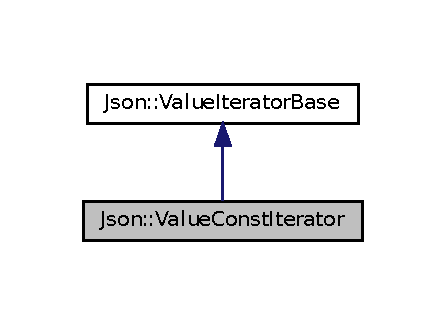
\includegraphics[width=214pt]{classJson_1_1ValueConstIterator__inherit__graph}
\end{center}
\end{figure}


Collaboration diagram for Json\+:\+:Value\+Const\+Iterator\+:
\nopagebreak
\begin{figure}[H]
\begin{center}
\leavevmode
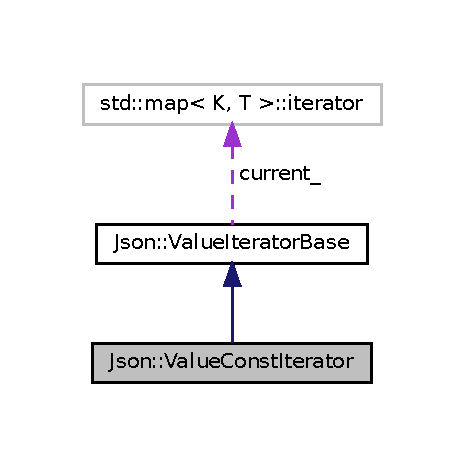
\includegraphics[width=214pt]{classJson_1_1ValueConstIterator__coll__graph}
\end{center}
\end{figure}
\subsection*{Public Types}
\begin{DoxyCompactItemize}
\item 
\mbox{\Hypertarget{classJson_1_1ValueConstIterator_aa5f1707dcef4bfe73e23ddc14dbe760d}\label{classJson_1_1ValueConstIterator_aa5f1707dcef4bfe73e23ddc14dbe760d}} 
typedef const \hyperlink{classJson_1_1Value}{Value} {\bfseries value\+\_\+type}
\item 
\mbox{\Hypertarget{classJson_1_1ValueConstIterator_aa9b05c6a37cd352ea1ee6e13b816f709}\label{classJson_1_1ValueConstIterator_aa9b05c6a37cd352ea1ee6e13b816f709}} 
typedef const \hyperlink{classJson_1_1Value}{Value} \& {\bfseries reference}
\item 
\mbox{\Hypertarget{classJson_1_1ValueConstIterator_a400136bd8bc09e9fddec0785fa2cff14}\label{classJson_1_1ValueConstIterator_a400136bd8bc09e9fddec0785fa2cff14}} 
typedef const \hyperlink{classJson_1_1Value}{Value} $\ast$ {\bfseries pointer}
\item 
\mbox{\Hypertarget{classJson_1_1ValueConstIterator_a0c2e33e7eb5a80dd8709fb28ece83933}\label{classJson_1_1ValueConstIterator_a0c2e33e7eb5a80dd8709fb28ece83933}} 
typedef \hyperlink{classJson_1_1ValueConstIterator}{Value\+Const\+Iterator} {\bfseries Self\+Type}
\end{DoxyCompactItemize}
\subsection*{Public Member Functions}
\begin{DoxyCompactItemize}
\item 
\mbox{\Hypertarget{classJson_1_1ValueConstIterator_a7ef3df204a9ae83a0d8a3cd128e05c70}\label{classJson_1_1ValueConstIterator_a7ef3df204a9ae83a0d8a3cd128e05c70}} 
{\bfseries Value\+Const\+Iterator} (\hyperlink{classJson_1_1ValueIterator}{Value\+Iterator} const \&other)
\item 
\mbox{\Hypertarget{classJson_1_1ValueConstIterator_ad1b1c11f8d7fb22d4d3c231915f2b15b}\label{classJson_1_1ValueConstIterator_ad1b1c11f8d7fb22d4d3c231915f2b15b}} 
\hyperlink{classJson_1_1ValueIteratorBase}{Self\+Type} \& {\bfseries operator=} (const \hyperlink{classJson_1_1ValueIteratorBase}{Value\+Iterator\+Base} \&other)
\item 
\mbox{\Hypertarget{classJson_1_1ValueConstIterator_ab3f0c2edbfc8f7d60645f3d597d05e28}\label{classJson_1_1ValueConstIterator_ab3f0c2edbfc8f7d60645f3d597d05e28}} 
\hyperlink{classJson_1_1ValueIteratorBase}{Self\+Type} {\bfseries operator++} (int)
\item 
\mbox{\Hypertarget{classJson_1_1ValueConstIterator_a94935961e9331c6f7b907b05ec8df75e}\label{classJson_1_1ValueConstIterator_a94935961e9331c6f7b907b05ec8df75e}} 
\hyperlink{classJson_1_1ValueIteratorBase}{Self\+Type} {\bfseries operator-\/-\/} (int)
\item 
\mbox{\Hypertarget{classJson_1_1ValueConstIterator_a31415e44e44e56fb2bfda7e8bb784646}\label{classJson_1_1ValueConstIterator_a31415e44e44e56fb2bfda7e8bb784646}} 
\hyperlink{classJson_1_1ValueIteratorBase}{Self\+Type} \& {\bfseries operator-\/-\/} ()
\item 
\mbox{\Hypertarget{classJson_1_1ValueConstIterator_a2cfe2f7a94a688186efdafb1b181c319}\label{classJson_1_1ValueConstIterator_a2cfe2f7a94a688186efdafb1b181c319}} 
\hyperlink{classJson_1_1ValueIteratorBase}{Self\+Type} \& {\bfseries operator++} ()
\item 
\mbox{\Hypertarget{classJson_1_1ValueConstIterator_ae5612dad47a6387eef71d584fb741d0c}\label{classJson_1_1ValueConstIterator_ae5612dad47a6387eef71d584fb741d0c}} 
\hyperlink{classJson_1_1Value}{reference} {\bfseries operator$\ast$} () const
\item 
\mbox{\Hypertarget{classJson_1_1ValueConstIterator_a3c608ae53c192ee846eb265bae1cfeec}\label{classJson_1_1ValueConstIterator_a3c608ae53c192ee846eb265bae1cfeec}} 
\hyperlink{classJson_1_1Value}{pointer} {\bfseries operator-\/$>$} () const
\end{DoxyCompactItemize}
\subsection*{Friends}
\begin{DoxyCompactItemize}
\item 
\mbox{\Hypertarget{classJson_1_1ValueConstIterator_aeceedf6e1a7d48a588516ce2b1983d6f}\label{classJson_1_1ValueConstIterator_aeceedf6e1a7d48a588516ce2b1983d6f}} 
class {\bfseries Value}
\end{DoxyCompactItemize}
\subsection*{Additional Inherited Members}


\subsection{Detailed Description}
const iterator for object and array value. 



The documentation for this class was generated from the following files\+:\begin{DoxyCompactItemize}
\item 
/home/mjonsson/repo/cpp\+Adv/media\+F\+W/inc/json/json.\+h\item 
/home/mjonsson/repo/cpp\+Adv/media\+F\+W/src/jsoncpp.\+cpp\end{DoxyCompactItemize}

\hypertarget{unionJson_1_1Value_1_1ValueHolder}{}\section{Json\+:\+:Value\+:\+:Value\+Holder Union Reference}
\label{unionJson_1_1Value_1_1ValueHolder}\index{Json\+::\+Value\+::\+Value\+Holder@{Json\+::\+Value\+::\+Value\+Holder}}


Collaboration diagram for Json\+:\+:Value\+:\+:Value\+Holder\+:
\nopagebreak
\begin{figure}[H]
\begin{center}
\leavevmode
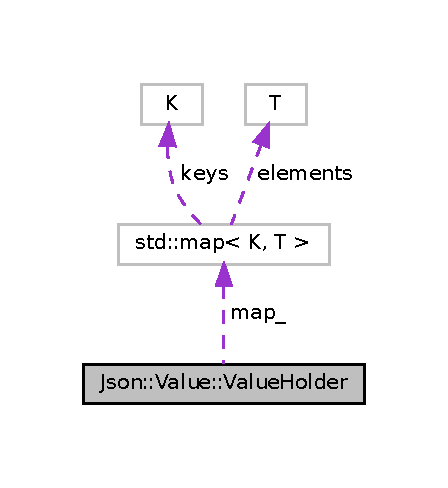
\includegraphics[width=215pt]{unionJson_1_1Value_1_1ValueHolder__coll__graph}
\end{center}
\end{figure}
\subsection*{Public Attributes}
\begin{DoxyCompactItemize}
\item 
\mbox{\Hypertarget{unionJson_1_1Value_1_1ValueHolder_adbfb384301298844ed955ba5cf6015a0}\label{unionJson_1_1Value_1_1ValueHolder_adbfb384301298844ed955ba5cf6015a0}} 
Largest\+Int {\bfseries int\+\_\+}
\item 
\mbox{\Hypertarget{unionJson_1_1Value_1_1ValueHolder_aab65665dc15a24a29a8e93cdeeaa7e50}\label{unionJson_1_1Value_1_1ValueHolder_aab65665dc15a24a29a8e93cdeeaa7e50}} 
Largest\+U\+Int {\bfseries uint\+\_\+}
\item 
\mbox{\Hypertarget{unionJson_1_1Value_1_1ValueHolder_af0c5ca724e5fe3a15db773d750e2351e}\label{unionJson_1_1Value_1_1ValueHolder_af0c5ca724e5fe3a15db773d750e2351e}} 
double {\bfseries real\+\_\+}
\item 
\mbox{\Hypertarget{unionJson_1_1Value_1_1ValueHolder_a92edab1861dadbfefd8be5fd4285eefe}\label{unionJson_1_1Value_1_1ValueHolder_a92edab1861dadbfefd8be5fd4285eefe}} 
bool {\bfseries bool\+\_\+}
\item 
\mbox{\Hypertarget{unionJson_1_1Value_1_1ValueHolder_a70ac2b153bc405527baa3850d2ddc3cb}\label{unionJson_1_1Value_1_1ValueHolder_a70ac2b153bc405527baa3850d2ddc3cb}} 
char $\ast$ {\bfseries string\+\_\+}
\item 
\mbox{\Hypertarget{unionJson_1_1Value_1_1ValueHolder_a1e7a5b86d4f52234f55c847ad1ce389a}\label{unionJson_1_1Value_1_1ValueHolder_a1e7a5b86d4f52234f55c847ad1ce389a}} 
Object\+Values $\ast$ {\bfseries map\+\_\+}
\end{DoxyCompactItemize}


The documentation for this union was generated from the following file\+:\begin{DoxyCompactItemize}
\item 
/home/mjonsson/repo/cpp\+Adv/media\+F\+W/inc/json/json.\+h\end{DoxyCompactItemize}

\hypertarget{classJson_1_1ValueIterator}{}\section{Json\+:\+:Value\+Iterator Class Reference}
\label{classJson_1_1ValueIterator}\index{Json\+::\+Value\+Iterator@{Json\+::\+Value\+Iterator}}


Iterator for object and array value.  




{\ttfamily \#include $<$json.\+h$>$}



Inheritance diagram for Json\+:\+:Value\+Iterator\+:
\nopagebreak
\begin{figure}[H]
\begin{center}
\leavevmode
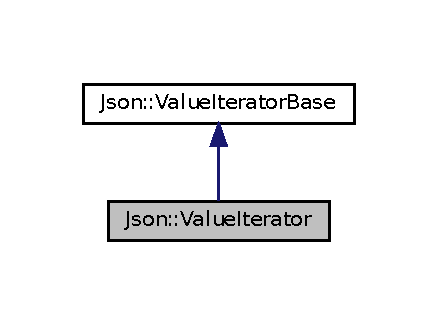
\includegraphics[width=210pt]{classJson_1_1ValueIterator__inherit__graph}
\end{center}
\end{figure}


Collaboration diagram for Json\+:\+:Value\+Iterator\+:
\nopagebreak
\begin{figure}[H]
\begin{center}
\leavevmode
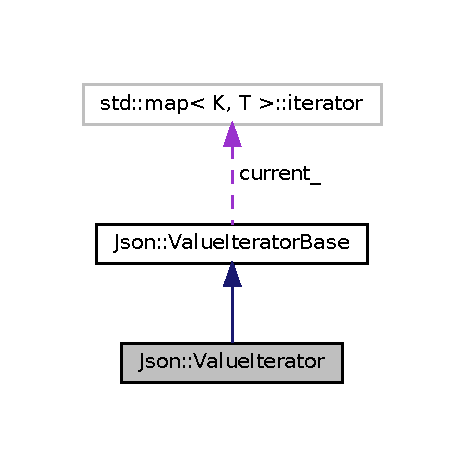
\includegraphics[width=210pt]{classJson_1_1ValueIterator__coll__graph}
\end{center}
\end{figure}
\subsection*{Public Types}
\begin{DoxyCompactItemize}
\item 
\mbox{\Hypertarget{classJson_1_1ValueIterator_a2c5ba7be611f05546530c8a88b2d2e37}\label{classJson_1_1ValueIterator_a2c5ba7be611f05546530c8a88b2d2e37}} 
typedef \hyperlink{classJson_1_1Value}{Value} {\bfseries value\+\_\+type}
\item 
\mbox{\Hypertarget{classJson_1_1ValueIterator_a308b8932ffc83eaa9d12dadd5c11a7dd}\label{classJson_1_1ValueIterator_a308b8932ffc83eaa9d12dadd5c11a7dd}} 
typedef unsigned int {\bfseries size\+\_\+t}
\item 
\mbox{\Hypertarget{classJson_1_1ValueIterator_a2be1a9aa60bbfc8812e9dd1a7f1a8786}\label{classJson_1_1ValueIterator_a2be1a9aa60bbfc8812e9dd1a7f1a8786}} 
typedef int {\bfseries difference\+\_\+type}
\item 
\mbox{\Hypertarget{classJson_1_1ValueIterator_ae87929b4567aa00372cf602c43b57160}\label{classJson_1_1ValueIterator_ae87929b4567aa00372cf602c43b57160}} 
typedef \hyperlink{classJson_1_1Value}{Value} \& {\bfseries reference}
\item 
\mbox{\Hypertarget{classJson_1_1ValueIterator_acec45feb1ef1f3bf81240157d06d5432}\label{classJson_1_1ValueIterator_acec45feb1ef1f3bf81240157d06d5432}} 
typedef \hyperlink{classJson_1_1Value}{Value} $\ast$ {\bfseries pointer}
\item 
\mbox{\Hypertarget{classJson_1_1ValueIterator_a23357670fdad61792670d86f62db7e16}\label{classJson_1_1ValueIterator_a23357670fdad61792670d86f62db7e16}} 
typedef \hyperlink{classJson_1_1ValueIterator}{Value\+Iterator} {\bfseries Self\+Type}
\end{DoxyCompactItemize}
\subsection*{Public Member Functions}
\begin{DoxyCompactItemize}
\item 
\mbox{\Hypertarget{classJson_1_1ValueIterator_aa85aa208670891670392259efa0143bb}\label{classJson_1_1ValueIterator_aa85aa208670891670392259efa0143bb}} 
{\bfseries Value\+Iterator} (const \hyperlink{classJson_1_1ValueConstIterator}{Value\+Const\+Iterator} \&other)
\item 
\mbox{\Hypertarget{classJson_1_1ValueIterator_a7d5e58a9a4a553968acdf3064b39d21c}\label{classJson_1_1ValueIterator_a7d5e58a9a4a553968acdf3064b39d21c}} 
{\bfseries Value\+Iterator} (const \hyperlink{classJson_1_1ValueIterator}{Value\+Iterator} \&other)
\item 
\mbox{\Hypertarget{classJson_1_1ValueIterator_a8e23312b1db874f7e403fd7e76611bdc}\label{classJson_1_1ValueIterator_a8e23312b1db874f7e403fd7e76611bdc}} 
\hyperlink{classJson_1_1ValueIteratorBase}{Self\+Type} \& {\bfseries operator=} (const \hyperlink{classJson_1_1ValueIteratorBase}{Self\+Type} \&other)
\item 
\mbox{\Hypertarget{classJson_1_1ValueIterator_abcf4ddd994a010742cd4a436d65acd08}\label{classJson_1_1ValueIterator_abcf4ddd994a010742cd4a436d65acd08}} 
\hyperlink{classJson_1_1ValueIteratorBase}{Self\+Type} {\bfseries operator++} (int)
\item 
\mbox{\Hypertarget{classJson_1_1ValueIterator_a06d6a29d96caf6af324a53973159e12b}\label{classJson_1_1ValueIterator_a06d6a29d96caf6af324a53973159e12b}} 
\hyperlink{classJson_1_1ValueIteratorBase}{Self\+Type} {\bfseries operator-\/-\/} (int)
\item 
\mbox{\Hypertarget{classJson_1_1ValueIterator_a811302a868518a0995a9def955df5720}\label{classJson_1_1ValueIterator_a811302a868518a0995a9def955df5720}} 
\hyperlink{classJson_1_1ValueIteratorBase}{Self\+Type} \& {\bfseries operator-\/-\/} ()
\item 
\mbox{\Hypertarget{classJson_1_1ValueIterator_a92146c46f8249e2b2d12869e70cd4cee}\label{classJson_1_1ValueIterator_a92146c46f8249e2b2d12869e70cd4cee}} 
\hyperlink{classJson_1_1ValueIteratorBase}{Self\+Type} \& {\bfseries operator++} ()
\item 
\mbox{\Hypertarget{classJson_1_1ValueIterator_a3be48b0c1729ec2532f1ff27ad465d32}\label{classJson_1_1ValueIterator_a3be48b0c1729ec2532f1ff27ad465d32}} 
\hyperlink{classJson_1_1Value}{reference} {\bfseries operator$\ast$} () const
\item 
\mbox{\Hypertarget{classJson_1_1ValueIterator_a8dfc1603f92467591d524d0326f35534}\label{classJson_1_1ValueIterator_a8dfc1603f92467591d524d0326f35534}} 
\hyperlink{classJson_1_1Value}{pointer} {\bfseries operator-\/$>$} () const
\end{DoxyCompactItemize}
\subsection*{Friends}
\begin{DoxyCompactItemize}
\item 
\mbox{\Hypertarget{classJson_1_1ValueIterator_aeceedf6e1a7d48a588516ce2b1983d6f}\label{classJson_1_1ValueIterator_aeceedf6e1a7d48a588516ce2b1983d6f}} 
class {\bfseries Value}
\end{DoxyCompactItemize}
\subsection*{Additional Inherited Members}


\subsection{Detailed Description}
Iterator for object and array value. 

The documentation for this class was generated from the following files\+:\begin{DoxyCompactItemize}
\item 
/home/mjonsson/repo/cpp\+Adv/media\+F\+W/inc/json/json.\+h\item 
/home/mjonsson/repo/cpp\+Adv/media\+F\+W/src/jsoncpp.\+cpp\end{DoxyCompactItemize}

\hypertarget{classJson_1_1ValueIteratorBase}{}\section{Json\+:\+:Value\+Iterator\+Base Class Reference}
\label{classJson_1_1ValueIteratorBase}\index{Json\+::\+Value\+Iterator\+Base@{Json\+::\+Value\+Iterator\+Base}}


base class for \hyperlink{classJson_1_1Value}{Value} iterators.  




{\ttfamily \#include $<$json.\+h$>$}



Inheritance diagram for Json\+:\+:Value\+Iterator\+Base\+:
\nopagebreak
\begin{figure}[H]
\begin{center}
\leavevmode
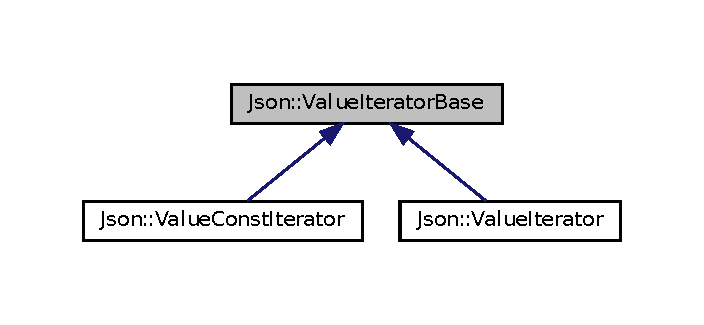
\includegraphics[width=338pt]{classJson_1_1ValueIteratorBase__inherit__graph}
\end{center}
\end{figure}
\subsection*{Public Types}
\begin{DoxyCompactItemize}
\item 
\mbox{\Hypertarget{classJson_1_1ValueIteratorBase_a02fd11a4fbdc0007da1e8bcf5e6b83c3}\label{classJson_1_1ValueIteratorBase_a02fd11a4fbdc0007da1e8bcf5e6b83c3}} 
typedef std\+::bidirectional\+\_\+iterator\+\_\+tag {\bfseries iterator\+\_\+category}
\item 
\mbox{\Hypertarget{classJson_1_1ValueIteratorBase_a9d3a3c7ce5cdefe23cb486239cf07bb5}\label{classJson_1_1ValueIteratorBase_a9d3a3c7ce5cdefe23cb486239cf07bb5}} 
typedef unsigned int {\bfseries size\+\_\+t}
\item 
\mbox{\Hypertarget{classJson_1_1ValueIteratorBase_a4e44bf8cbd17ec8d6e2c185904a15ebd}\label{classJson_1_1ValueIteratorBase_a4e44bf8cbd17ec8d6e2c185904a15ebd}} 
typedef int {\bfseries difference\+\_\+type}
\item 
\mbox{\Hypertarget{classJson_1_1ValueIteratorBase_a9d2a940d03ea06d20d972f41a89149ee}\label{classJson_1_1ValueIteratorBase_a9d2a940d03ea06d20d972f41a89149ee}} 
typedef \hyperlink{classJson_1_1ValueIteratorBase}{Value\+Iterator\+Base} {\bfseries Self\+Type}
\end{DoxyCompactItemize}
\subsection*{Public Member Functions}
\begin{DoxyCompactItemize}
\item 
\mbox{\Hypertarget{classJson_1_1ValueIteratorBase_a1248d8016f88b51371a0fcbd355b3cfd}\label{classJson_1_1ValueIteratorBase_a1248d8016f88b51371a0fcbd355b3cfd}} 
bool {\bfseries operator==} (const \hyperlink{classJson_1_1ValueIteratorBase}{Self\+Type} \&other) const
\item 
\mbox{\Hypertarget{classJson_1_1ValueIteratorBase_aa83bdcc8114b7d040eb8eb42eeed5f4a}\label{classJson_1_1ValueIteratorBase_aa83bdcc8114b7d040eb8eb42eeed5f4a}} 
bool {\bfseries operator!=} (const \hyperlink{classJson_1_1ValueIteratorBase}{Self\+Type} \&other) const
\item 
\mbox{\Hypertarget{classJson_1_1ValueIteratorBase_a98e254263fca5f1fc8fcac7bcb0260bf}\label{classJson_1_1ValueIteratorBase_a98e254263fca5f1fc8fcac7bcb0260bf}} 
difference\+\_\+type {\bfseries operator-\/} (const \hyperlink{classJson_1_1ValueIteratorBase}{Self\+Type} \&other) const
\item 
\hyperlink{classJson_1_1Value}{Value} \hyperlink{classJson_1_1ValueIteratorBase_a3838ba39c43c518cf3ed4aa6ce78ccad}{key} () const
\item 
U\+Int \hyperlink{classJson_1_1ValueIteratorBase_a549c66a0bd20e9ae772175a5c0d2e88a}{index} () const
\item 
J\+S\+O\+N\+C\+P\+P\+\_\+\+S\+T\+R\+I\+NG \hyperlink{classJson_1_1ValueIteratorBase_a522989403c976fdbb94da846b99418db}{name} () const
\item 
char const  $\ast$ \hyperlink{classJson_1_1ValueIteratorBase_a54765da6759fd3f1edcbfbaf308ec263}{member\+Name} () const
\item 
char const  $\ast$ \hyperlink{classJson_1_1ValueIteratorBase_a391c9cbd0edf9a447b37df00e8ce6059}{member\+Name} (char const $\ast$$\ast$end) const
\item 
\mbox{\Hypertarget{classJson_1_1ValueIteratorBase_a640e990e5f03a96fd650122a2906f59d}\label{classJson_1_1ValueIteratorBase_a640e990e5f03a96fd650122a2906f59d}} 
{\bfseries Value\+Iterator\+Base} (const Value\+::\+Object\+Values\+::iterator \&current)
\end{DoxyCompactItemize}
\subsection*{Protected Member Functions}
\begin{DoxyCompactItemize}
\item 
\mbox{\Hypertarget{classJson_1_1ValueIteratorBase_aa5b75c9514a30ba2ea3c9a35c165c18e}\label{classJson_1_1ValueIteratorBase_aa5b75c9514a30ba2ea3c9a35c165c18e}} 
\hyperlink{classJson_1_1Value}{Value} \& {\bfseries deref} () const
\item 
\mbox{\Hypertarget{classJson_1_1ValueIteratorBase_afe58f9534e1fd2033419fd9fe244551e}\label{classJson_1_1ValueIteratorBase_afe58f9534e1fd2033419fd9fe244551e}} 
void {\bfseries increment} ()
\item 
\mbox{\Hypertarget{classJson_1_1ValueIteratorBase_affc8cf5ff54a9f432cc693362c153fa6}\label{classJson_1_1ValueIteratorBase_affc8cf5ff54a9f432cc693362c153fa6}} 
void {\bfseries decrement} ()
\item 
\mbox{\Hypertarget{classJson_1_1ValueIteratorBase_af11473c9e20d07782e42b52a2f9e4540}\label{classJson_1_1ValueIteratorBase_af11473c9e20d07782e42b52a2f9e4540}} 
difference\+\_\+type {\bfseries compute\+Distance} (const \hyperlink{classJson_1_1ValueIteratorBase}{Self\+Type} \&other) const
\item 
\mbox{\Hypertarget{classJson_1_1ValueIteratorBase_a010b5ad3f3337ae3732e5d7e16ca5e25}\label{classJson_1_1ValueIteratorBase_a010b5ad3f3337ae3732e5d7e16ca5e25}} 
bool {\bfseries is\+Equal} (const \hyperlink{classJson_1_1ValueIteratorBase}{Self\+Type} \&other) const
\item 
\mbox{\Hypertarget{classJson_1_1ValueIteratorBase_a496e6aba44808433ec5858c178be5719}\label{classJson_1_1ValueIteratorBase_a496e6aba44808433ec5858c178be5719}} 
void {\bfseries copy} (const \hyperlink{classJson_1_1ValueIteratorBase}{Self\+Type} \&other)
\end{DoxyCompactItemize}


\subsection{Detailed Description}
base class for \hyperlink{classJson_1_1Value}{Value} iterators. 



\subsection{Member Function Documentation}
\mbox{\Hypertarget{classJson_1_1ValueIteratorBase_a549c66a0bd20e9ae772175a5c0d2e88a}\label{classJson_1_1ValueIteratorBase_a549c66a0bd20e9ae772175a5c0d2e88a}} 
\index{Json\+::\+Value\+Iterator\+Base@{Json\+::\+Value\+Iterator\+Base}!index@{index}}
\index{index@{index}!Json\+::\+Value\+Iterator\+Base@{Json\+::\+Value\+Iterator\+Base}}
\subsubsection{\texorpdfstring{index()}{index()}}
{\footnotesize\ttfamily U\+Int Json\+::\+Value\+Iterator\+Base\+::index (\begin{DoxyParamCaption}{ }\end{DoxyParamCaption}) const}

Return the index of the referenced \hyperlink{classJson_1_1Value}{Value}, or -\/1 if it is not an array\+Value. \mbox{\Hypertarget{classJson_1_1ValueIteratorBase_a3838ba39c43c518cf3ed4aa6ce78ccad}\label{classJson_1_1ValueIteratorBase_a3838ba39c43c518cf3ed4aa6ce78ccad}} 
\index{Json\+::\+Value\+Iterator\+Base@{Json\+::\+Value\+Iterator\+Base}!key@{key}}
\index{key@{key}!Json\+::\+Value\+Iterator\+Base@{Json\+::\+Value\+Iterator\+Base}}
\subsubsection{\texorpdfstring{key()}{key()}}
{\footnotesize\ttfamily \hyperlink{classJson_1_1Value}{Value} Json\+::\+Value\+Iterator\+Base\+::key (\begin{DoxyParamCaption}{ }\end{DoxyParamCaption}) const}

Return either the index or the member name of the referenced value as a \hyperlink{classJson_1_1Value}{Value}. \mbox{\Hypertarget{classJson_1_1ValueIteratorBase_a54765da6759fd3f1edcbfbaf308ec263}\label{classJson_1_1ValueIteratorBase_a54765da6759fd3f1edcbfbaf308ec263}} 
\index{Json\+::\+Value\+Iterator\+Base@{Json\+::\+Value\+Iterator\+Base}!member\+Name@{member\+Name}}
\index{member\+Name@{member\+Name}!Json\+::\+Value\+Iterator\+Base@{Json\+::\+Value\+Iterator\+Base}}
\subsubsection{\texorpdfstring{member\+Name()}{memberName()}\hspace{0.1cm}{\footnotesize\ttfamily [1/2]}}
{\footnotesize\ttfamily char const  $\ast$ Json\+::\+Value\+Iterator\+Base\+::member\+Name (\begin{DoxyParamCaption}{ }\end{DoxyParamCaption}) const}

Return the member name of the referenced \hyperlink{classJson_1_1Value}{Value}. \char`\"{}\char`\"{} if it is not an object\+Value. \begin{DoxyRefDesc}{Deprecated}
\item[\hyperlink{deprecated__deprecated000004}{Deprecated}]This cannot be used for U\+T\+F-\/8 strings, since there can be embedded nulls. \end{DoxyRefDesc}
\mbox{\Hypertarget{classJson_1_1ValueIteratorBase_a391c9cbd0edf9a447b37df00e8ce6059}\label{classJson_1_1ValueIteratorBase_a391c9cbd0edf9a447b37df00e8ce6059}} 
\index{Json\+::\+Value\+Iterator\+Base@{Json\+::\+Value\+Iterator\+Base}!member\+Name@{member\+Name}}
\index{member\+Name@{member\+Name}!Json\+::\+Value\+Iterator\+Base@{Json\+::\+Value\+Iterator\+Base}}
\subsubsection{\texorpdfstring{member\+Name()}{memberName()}\hspace{0.1cm}{\footnotesize\ttfamily [2/2]}}
{\footnotesize\ttfamily char const  $\ast$ Json\+::\+Value\+Iterator\+Base\+::member\+Name (\begin{DoxyParamCaption}\item[{char const $\ast$$\ast$}]{end }\end{DoxyParamCaption}) const}

Return the member name of the referenced \hyperlink{classJson_1_1Value}{Value}, or N\+U\+LL if it is not an object\+Value. \begin{DoxyNote}{Note}
Better version than \hyperlink{classJson_1_1ValueIteratorBase_a54765da6759fd3f1edcbfbaf308ec263}{member\+Name()}. Allows embedded nulls. 
\end{DoxyNote}
\mbox{\Hypertarget{classJson_1_1ValueIteratorBase_a522989403c976fdbb94da846b99418db}\label{classJson_1_1ValueIteratorBase_a522989403c976fdbb94da846b99418db}} 
\index{Json\+::\+Value\+Iterator\+Base@{Json\+::\+Value\+Iterator\+Base}!name@{name}}
\index{name@{name}!Json\+::\+Value\+Iterator\+Base@{Json\+::\+Value\+Iterator\+Base}}
\subsubsection{\texorpdfstring{name()}{name()}}
{\footnotesize\ttfamily J\+S\+O\+N\+C\+P\+P\+\_\+\+S\+T\+R\+I\+NG Json\+::\+Value\+Iterator\+Base\+::name (\begin{DoxyParamCaption}{ }\end{DoxyParamCaption}) const}

Return the member name of the referenced \hyperlink{classJson_1_1Value}{Value}, or \char`\"{}\char`\"{} if it is not an object\+Value. \begin{DoxyNote}{Note}
Avoid {\ttfamily c\+\_\+str()} on result, as embedded zeroes are possible. 
\end{DoxyNote}


The documentation for this class was generated from the following files\+:\begin{DoxyCompactItemize}
\item 
/home/mjonsson/repo/cpp\+Adv/media\+F\+W/inc/json/json.\+h\item 
/home/mjonsson/repo/cpp\+Adv/media\+F\+W/src/jsoncpp.\+cpp\end{DoxyCompactItemize}

%--- End generated contents ---

% Index
\backmatter
\newpage
\phantomsection
\clearemptydoublepage
\addcontentsline{toc}{chapter}{Index}
\printindex

\end{document}
